\documentclass[a4paper,8pt,titlepage]{scrbook}

\usepackage[T1]{fontenc}
\usepackage[utf8]{inputenc}
\usepackage[ngerman]{babel}
\usepackage{hyperref}
\usepackage{tabularx}
\usepackage{amsmath}
\usepackage{amssymb}
\usepackage{graphicx}
\usepackage{listings}
\usepackage[ruled,vlined]{algorithm2e}
\usepackage{esdiff}
\usepackage{float}
\usepackage{geometry}
\geometry{left=2cm,right=2cm,top=2cm,bottom=2cm,bindingoffset=10mm}
\restylefloat{table}
% Taken from http://blog.virtualglobebook.com/2011/02/syntax-highlighting-c-and-glsl-source.html
\lstdefinelanguage{GLSL} {
	sensitive=true,
	morekeywords=[1]{
	attribute, const, uniform, varying,
	layout, centroid, flat, smooth,
	noperspective, break, continue, do,
	for, while, switch, case, default, if,
	else, in, out, inout, float, int, void,
	bool, true, false, invariant, discard,
	return, mat2, mat3, mat4, mat2x2, mat2x3,
	mat2x4, mat3x2, mat3x3, mat3x4, mat4x2,
	mat4x3, mat4x4, vec2, vec3, vec4, ivec2,
	ivec3, ivec4, bvec2, bvec3, bvec4, uint,
	uvec2, uvec3, uvec4, lowp, mediump, highp,
	precision, sampler1D, sampler2D, sampler3D,
	samplerCube, sampler1DShadow,
	sampler2DShadow, samplerCubeShadow,
	sampler1DArray, sampler2DArray,
	sampler1DArrayShadow, sampler2DArrayShadow,
	isampler1D, isampler2D, isampler3D,
	isamplerCube, isampler1DArray,
	isampler2DArray, usampler1D, usampler2D,
	usampler3D, usamplerCube, usampler1DArray,
	usampler2DArray, sampler2DRect,
	sampler2DRectShadow, isampler2DRect,
	usampler2DRect, samplerBuffer,
	isamplerBuffer, usamplerBuffer, sampler2DMS,
	isampler2DMS, usampler2DMS,
	sampler2DMSArray, isampler2DMSArray,
	usampler2DMSArray, struct},
	morekeywords=[2]{
	radians,degrees,sin,cos,tan,asin,acos,atan,
	atan,sinh,cosh,tanh,asinh,acosh,atanh,pow,
	exp,log,exp2,log2,sqrt,inversesqrt,abs,sign,
	floor,trunc,round,roundEven,ceil,fract,mod,modf,
	min,max,clamp,mix,step,smoothstep,isnan,isinf,
	floatBitsToInt,floatBitsToUint,intBitsToFloat,
	uintBitsToFloat,length,distance,dot,cross,
	normalize,faceforward,reflect,refract,
	matrixCompMult,outerProduct,transpose,
	determinant,inverse,lessThan,lessThanEqual,
	greaterThan,greaterThanEqual,equal,notEqual,
	any,all,not,textureSize,texture,textureProj,
	textureLod,textureOffset,texelFetch,
	texelFetchOffset,textureProjOffset,
	textureLodOffset,textureProjLod,
	textureProjLodOffset,textureGrad,
	textureGradOffset,textureProjGrad,
	textureProjGradOffset,texture1D,texture1DProj,
	texture1DProjLod,texture2D,texture2DProj,
	texture2DLod,texture2DProjLod,texture3D,
	texture3DProj,texture3DLod,texture3DProjLod,
	textureCube,textureCubeLod,shadow1D,shadow2D,
	shadow1DProj,shadow2DProj,shadow1DLod,
	shadow2DLod,shadow1DProjLod,shadow2DProjLod,
	dFdx,dFdy,fwidth,noise1,noise2,noise3,noise4,
	EmitVertex,EndPrimitive},
	morekeywords=[3]{
	gl_VertexID,gl_InstanceID,gl_Position,
	gl_PointSize,gl_ClipDistance,gl_PerVertex,
	gl_Layer,gl_ClipVertex,gl_FragCoord,
	gl_FrontFacing,gl_ClipDistance,gl_FragColor,
	gl_FragData,gl_MaxDrawBuffers,gl_FragDepth,
	gl_PointCoord,gl_PrimitiveID,
	gl_MaxVertexAttribs,gl_MaxVertexUniformComponents,
	gl_MaxVaryingFloats,gl_MaxVaryingComponents,
	gl_MaxVertexOutputComponents,
	gl_MaxGeometryInputComponents,
	gl_MaxGeometryOutputComponents,
	gl_MaxFragmentInputComponents,
	gl_MaxVertexTextureImageUnits,
	gl_MaxCombinedTextureImageUnits,
	gl_MaxTextureImageUnits,
	gl_MaxFragmentUniformComponents,
	gl_MaxDrawBuffers,gl_MaxClipDistances,
	gl_MaxGeometryTextureImageUnits,
	gl_MaxGeometryOutputVertices,
	gl_MaxGeometryOutputVertices,
	gl_MaxGeometryTotalOutputComponents,
	gl_MaxGeometryUniformComponents,
	gl_MaxGeometryVaryingComponents,gl_DepthRange},
	morecomment=[l]{//},
	morecomment=[s]{/*}{*/},
	morecomment=[l][keywordstyle4]{\#},
}

\title{Vorlesungen am Karlsruher Institut für Technologie}
\author{Maximilian Heß}
\date{Februar 2016}

\begin{document}
\maketitle
\tableofcontents

\part{Bachelor}
\chapter{Algorithmen II}

Zusammenfassung der Vorlesung "`Algorithmen II"' aus dem Wintersemester 2014.\footnote{\url{http://geom.ivd.kit.edu/ws14_algo2.php}}


\section{Flussmaximierung}

\subsection{Flussnetzwerke}
\textbf{Ziel:} Berechnung des maximalen Flusses.

\subsubsection{Bestandteile}
\begin{itemize}
	\item Graph mit Quelle \(q\) und Senke \(s\): \(G(V,E)\) mit \(E \subset V^2\)
	\item Kapazitätsfunktion \(k : V^2 \rightarrow \mathbb{R}_{+0}\), wobei \(\forall e \in V^2 \setminus E: k(e) = 0\)
\end{itemize}

\subsubsection{Flüsse}
Ein Fluss in F ist eine Funktion \(f:V^2\rightarrow\mathbb{R}\) mit den Eigenschaften:
\begin{enumerate}
	\item \(f \leq k\)
	\item \(\forall x,y \in V : f(x,y) = -f(y,x)\)
	\item \(\forall x \in V \setminus \{ q,s \}: 0 = \sum f(x,V) := \sum_{y\in V} f(x,y)\)
\end{enumerate}
\paragraph{Flusserhalt} Wegen (2) bedeutet (3), dass in jeden Knoten außer \(q\) und \(s\) soviel positiver Fluss rein- wie rausfließt.

\subsubsection{Bemerkungen}
\begin{itemize}
	\item Der maximale Fluss ist die Summe der von der Quelle ausgehenden / bei der Senke ankommenden genutzen Kapazitäten / der minimale Schnitt durch den Graphen
	\item Der negative Fluss soll lediglich die Darstellung vereinfachen und ist ansonsten uninteressant
	\item In alle Knoten außer in \(q\) und in \(s\) fließt immer so viel positiver Fluss rein wie raus (wegen (2) bedeutet (3) Flusserhalt)
	\item Mehrere Flussnetzwerke können zu einem Flussnetzwerk zusammengefasst werden (mit unendlichen Zu- und Abflüssen)
	\item Residualgraph: Der Graph der Restkapazität
\end{itemize}


\subsection{Algorithmus von Ford und Fulkerson}
\begin{itemize}
	\item \textbf{Algorithmus}
	\begin{enumerate}
		\item Setze die Flüsse an allen Kanten gleich Null
		\item Solange es einen Pfad von \(q\) nach \(s\) gibt, erhöhe diesen maximal
	\end{enumerate}
	\item Terminiert Ford-Fulkerson, ist \(f\) maximal, da es keinen weiteren Pfad \(q \rightarrow^{*} s\) gibt
	\item Aufwand: \(\mathcal{O}(|E| \cdot max\{W_f | f~Fluss~in~F\})\), denn ein Pfad \(q \rightarrow^{*} s\) kann in \(|E|\) Schritten gefunden werden
\end{itemize}
\begin{algorithm}[H]
	\caption{Ford-Fulkerson}
	\SetKwData{Left}{left}\SetKwData{This}{this}\SetKwData{Up}{up}
	\SetKwFunction{Union}{Union}\SetKwFunction{FindCompress}{FindCompress}
	\SetKwInOut{Input}{input}\SetKwInOut{Output}{output}

	\Input{$F(G,k,q,s)$}
	\Output{Ein maximaler Fluß $f$}
	\BlankLine

	$f \longleftarrow 0$

	\While{Es gibt einen Pfad $q \rightarrow^* s$ in $G_f$} {
		Erhöhe $f$ über diesen maximal
	}
\end{algorithm}


\subsection{Algorithmus von Edmonds und Karp}
\begin{itemize}
	\item Idee: Anwendung von Ford-Fulkerson immer längs eines kürzesten Pfades (Breitensuche)
	\item Terminiert auch für beliebige reelle Kapazitäten
	\item In jedem Schritt verliert \(E_f\) eine Kante
	\item Aufwand: \(\mathcal{O} (|E|^2 \cdot |V|)\)
\end{itemize}


\subsection{Präfluss-Pusch-Methode}
Jeder Knoten erhält zusätzlich eine Höhe und ein Reservoir, um vorübergehend beliebig viel Fluß speichern zu können.

\subsubsection{Operationen}

\paragraph{\(PUSCH(x,y)\)}
\begin{itemize}
	\item \textbf{Bedingungen}
	\begin{itemize}
		\item Überschuss bei \(x\) vorhanden: \(u(x) > 0, x \in V \setminus \{q,s\}\)
		\item \(x\) liegt höher als \(y\): \(h(x) - h(y) \leq 1\)
	\end{itemize}
	\item \textbf{Algorithmus}
	\begin{enumerate}
		\item Ermittle den Abfluss aus Überschuss und Restkapazität: \(min\{u(x), k_f(x,y)\}\)
		\item Erhöhe den Fluss auf der Kante \((x,y)\)
		\item Aktualisiere die Überschusswerte an \(x\) und \(y\)
	\end{enumerate}
\end{itemize}
\begin{algorithm}[H]
	\caption{Push}
	\SetKwData{Left}{left}\SetKwData{This}{this}\SetKwData{Up}{up}
	\SetKwFunction{Union}{Union}\SetKwFunction{FindCompress}{FindCompress}
	\SetKwInOut{Input}{input}\SetKwInOut{Output}{output}

	\Input{$x,y$}
	\Output{}
	\BlankLine

	$d \longleftarrow \min\{u(x), k_f(x,y)\}$ \newline
	$f(x,y) \longleftarrow f(x,y) + d$ \newline
	$u(x) \longleftarrow u(x) - d $ \newline
	$u(y) \longleftarrow u(y) + d$ \newline
\end{algorithm}

\paragraph{\(LIFTE(x)\)}
\begin{itemize}
	\item \textbf{Bedingungen}
	\begin{itemize}
		\item Der Knoten ist weder \(q\) und \(s\)
		\item Überschuss bei \(x\) vorhanden
		\item \(x\) kann nur geliftet werden, wenn kein Pfad \(y \rightarrow x\) eine höhere Restkapazität aufweist: \(h(x) < h(y)\)
	\end{itemize}
	\item \textbf{Algorithmus}
	\begin{enumerate}
		\item Erhöhe \(x\): \(h(x) = 1 + min\{h(y)\}\)
	\end{enumerate}
\end{itemize}
\begin{algorithm}[H]
	\caption{Lifte}
	\SetKwData{Left}{left}\SetKwData{This}{this}\SetKwData{Up}{up}
	\SetKwFunction{Union}{Union}\SetKwFunction{FindCompress}{FindCompress}
	\SetKwInOut{Input}{input}\SetKwInOut{Output}{output}

	\Input{$x$}
	\BlankLine

	$h(x) := 1+ \min_{(x,y) \in E_f}{h(y)}$
\end{algorithm}

\paragraph{Durchführung}
\begin{enumerate}
	\item \textbf{Initialisiere}
	\begin{enumerate}
		\item Alle Knoten außer \(q\) wird \(h=0\) zugewiesen (\(h(q) = |V|)\)
		\item Alle von \(q\) ausgehenden Pfade bekommen die Kapazität nach \(k(x,y)\) zugewiesen, alle anderen Pfade \(0\)
	\end{enumerate}
	\item Solange es eine beliebige, erlaubte Operation gibt, führe diese aus
\end{enumerate}
\begin{algorithm}[H]
	\caption{Präfluss-Pusch}
	\SetKwData{Left}{left}\SetKwData{This}{this}\SetKwData{Up}{up}
	\SetKwFunction{Union}{Union}\SetKwFunction{FindCompress}{FindCompress}
	\SetKwInOut{Input}{input}\SetKwInOut{Output}{output}

	\Input{$F(G,k,q,s)$}
	\Output{Maximaler Fluss $f$}
	\BlankLine

	\For{alle $ x,y \in V $ }{
	$ h(x)  \leftarrow \begin{cases}|V| & x=q \\ 0 & \text{sonst}\end{cases}$ \newline
	$ f(x,y)  \leftarrow \begin{cases}k(x,y) & x=q \\ 0 & \text{sonst}\end{cases}$}
	\While{Es gibt erlaubte Push oder Lifte Operationen}{
		Führe diese \textit{Pusch}- oder \textit{Lifte}-Operation aus
	}
\end{algorithm}

\subsubsection{Laufzeit}
\[\mathcal{O} (|V|^2 \cdot |E|)\]


\subsection{Move-to-Front-Algorithmus}
Durch eine strukturierte Abarbeitung der Operationen wird \textit{Präfluss-Pusch} beschleunigt.

\begin{itemize}
	\item Idee: Strukturiertes Entladen der Knoten
	\item Die Nachbarn von \(x\) werden über eine invertierte Liste verwaltet
	\item \((x,y) \in E\) heißt \textit{puschbar}, falls \(k_f(x,y) \geq 0\) und \(h(x)-h(y)\geq 1\)
	\item Die Knoten werden über eine Liste verwaltet, in der \(x\) vor \(y\) auftritt, falls \((x,y)\) \textit{PUSCHBAR} ist
	\item Geliftete Knoten werden an die Spitze der Listen gesetzt
\end{itemize}

\subsubsection{Operationen}
\begin{algorithm}[H]
	\caption{Leere}
	\SetKwData{Left}{left}\SetKwData{This}{this}\SetKwData{Up}{up}
	\SetKwFunction{Union}{Union}\SetKwFunction{FindCompress}{FindCompress}
	\SetKwInOut{Input}{input}\SetKwInOut{Output}{output}

	\Input{$x$}
	\BlankLine

	\While{$u(x)>0$}{	
		\eIf{$i_x > 0$}{
			$y \longleftarrow n_x(i_x)$ \newline
			\eIf{$(x,y)~puschbar$}{
				$Pusch(x,y)$
			}{
				$i_x \longleftarrow i_x -1$}
		}{	$Lifte(x)$ \newline
				$i_x \longleftarrow Grad(x)$}
			
		}	
\end{algorithm}
\text{}\\
\begin{algorithm}[H]
	\caption{An die Spitze}
	\SetKwData{Left}{left}\SetKwData{This}{this}\SetKwData{Up}{up}
	\SetKwFunction{Union}{Union}\SetKwFunction{FindCompress}{FindCompress}
	\SetKwInOut{Input}{input}\SetKwInOut{Output}{output}

	\Input{$F(G,k,q,s)$}
	\Output{Ein maximaler Fluss $f$}
	\BlankLine
	
	Initialisiere $f$ und $h$ wie in Präfluss-Pusch \newline
	Generiere $L$ \newline
	$x \longleftarrow Kopf(L)$
	\BlankLine

	\For{$x \in V$}{
		$i_x \longleftarrow Grad(x)$}
	\BlankLine

	\While{$x \ne Nil$ }{	
		$h_{alt} \longleftarrow h(x)$ \newline
		$Leere(x)$ \newline
		\If{$h_{alt} < h(x)$}{
			Setze $x$ an die Spitze von $L$
		}
		\BlankLine
		$x \longleftarrow \text{Nachfolger von x in L}$
	}
\end{algorithm}

\subsubsection{Laufzeit}
\[\mathcal{O}(|V|^3)\]



\section{Zuordnungsprobleme}
\textbf{Ziel:} Verteilung verschiedener Aufgaben auf eine Gruppe von Personen mit unterschiedlichen Fähigkeiten.

\subsection{Paaren in bipartiten Graphen}
\begin{itemize}
	\item Eine Paarung beinhaltet zwei Knoten exklusiv
	\item Eine Paarung heißt maximal, wenn es keine bessere Paarung gibt
	\item Maximale Paarung über Flußmaximierung: Ergänzung des bipartiten Graphs um Quelle und Senke
\end{itemize}


\subsection{Paaren in allgemeinen Graphen}
Sei \(G=(V,E)\) ein Graph mit einer Paarung \(P\) und einer maximalen Paarung \(Q\).

\subsubsection{Symmetrische Differenz}
\[D:=(P\setminus Q) \cup (Q \setminus P)\]
Die Kanten dieser Wege liegen alternierend in \(P\) und \(Q\) \(\rightarrow\) Zyklen haben eine gerade Länge.

\subsubsection{Definition}
Es gibt \(k= |Q|-|P|=|Q\setminus (P \cap Q)| - |P\setminus (P \cap Q)|\) Wege, auf denen \(P\) vergrößert werden kann. Die Endkanten liegen beiden \(\in Q\).

\subsubsection{Folgerung}
Man kann eine maximale Paarung durch sukzessive Vergrößerungen finden.

\paragraph{Algorithmus zur Vergößerung}
\begin{enumerate}
	\item Suche \((x,y) \in E\), wobei \(x\) mit keinem \(z\in V\) gepaart
	\item Setze \((x,y)\) durch Breitensuche zu einem alternierden Weg \(W\) ungerade Länge fort
\end{enumerate}
\begin{algorithm}[H]
	\caption{Paare}
	\SetKwData{Left}{left}\SetKwData{This}{this}\SetKwData{Up}{up}
	\SetKwFunction{Union}{Union}\SetKwFunction{FindCompress}{FindCompress}
	\SetKwInOut{Input}{input}\SetKwInOut{Output}{output}

	\Input{bipartiter Graph $(V_1 \stackrel{\cdot}{\cup} V_2, E)$}
	\Output{Maximale Paarung P}
	\BlankLine
	
	$V \longleftarrow V_1 \cup V_2 \cup \{ q,s \}$ \newline
	$\hat{E} \longleftarrow \{ q \} \times V_1 \cup E \cup V_2 \times \{ s \} $ \newline
	\BlankLine

	\tcc{Initialisiere alle Kanten mit Kapazität $1$}
	$k \longleftarrow \begin{cases}1 & e \in \hat{E} \\ 0 & \text{sonst}\end{cases}$ \newline
	\BlankLine

	$f \longleftarrow Ford-Fulkerson( F(V, \hat{E} ),h,q,s)) $ \newline
	\BlankLine

	\tcc{Die Kanten mit Fluss $1$ im Ursprungsgraphen bilden die maximale Paarung}
	$P \longleftarrow \{ e \in E~|~f(e) = 1 \} $
\end{algorithm}

\subsubsection{Blüten}
\begin{itemize}
	\item Zu Problemen kommt es bei sogenannten Blüten
	\item Lösung: Man schrumpft die Blüten ohne ihren Stil zu einem Knoten
\end{itemize}

\subsubsection{Aufwand der Suche nach vergrößernden Wegen}
\[\mathcal{O}(\sqrt{|V|} \cdot |E|)\]


\subsection{Maximal gewichtete Paarung}
\textbf{Gesucht:} Maximal gewichtete Paarung eines ungerichteten Graph:
\[\Gamma(P) := \Sigma \gamma (P)\]

\subsubsection{Annahme}
Man kann eine maximal gewichtete Paarung finden, indem eine maximal gewichtete Kante iterativ durch einen vergrößernden Weg zu einer nächstgrößeren Paarung vergrößert wird.

\paragraph{Aufwand}
\[\mathcal{O}(min\{|V|^3, |V| \cdot |E| \cdot log|V|\})\]



\section{Stochastische Algorithmen}

\subsubsection{Begriffe}
\begin{itemize}
	\item Las-Vegas-Algorithmus: Randomisierter Algorithmus, der immer ein korrektes Ergebnis liefert, wenn er terminiert.\footnote{\url{http://de.wikipedia.org/wiki/Las-Vegas-Algorithmus}}
	\item Monte-Carlo-Algorithmus: Randomisierte Algorithmen, die mit einer nach oben beschränkten Wahrscheinlichkeit ein falsches Ergebnis liefern dürfen. Dafür sind sie im Vergleich zu deterministischen Algorithmen häufig effizienter.\footnote{\url{http://de.wikipedia.org/wiki/Monte-Carlo-Algorithmus}}
\end{itemize}

\subsection{Erwartungswert}
Der Erwartungswert einer Zufallsvariablen beschreibt die Zahl, die die Zufallsvariable im Mittel annimmt.\footnote{\url{http://de.wikipedia.org/wiki/Erwartungswert}}

\subsubsection{Sigma-Additivität}
\[\mathbb{E}\lbrack \Sigma X_i\rbrack = \Sigma E \lbrack X_i\rbrack\]


\subsection{Quicksort}
\begin{itemize}
	\item Sortieren durch stochastisches Teilen
	\item Aufwandsabschätzung anhand der durchgeführten Vergleiche
\end{itemize}
\begin{algorithm}[H]
	\caption{Quicksort}
	\SetKwData{Left}{left}\SetKwData{This}{this}\SetKwData{Up}{up}
	\SetKwFunction{Union}{Union}\SetKwFunction{FindCompress}{FindCompress}
	\SetKwInOut{Input}{input}\SetKwInOut{Output}{output}

	\Input{$ S : = \{ s_1, ... , s_n \} $ 	mit paarweise verschiedenen 	$ s_i \in \mathbb{Z} $ 	}
	\Output{$(\sigma_1,...,\sigma_n)$ mit $\sigma_1 < ... < \sigma_n$ und $\{\sigma_1, ... , \sigma_n \} = S $}
	\BlankLine
	
	\While{ S $\ne \emptyset$} {
		Wähle ein zufälliges Pivotelement $ y \in S $ \newline
		Zerlege $S \setminus \{ y \} $ 	in 	$  s_1 $ und $ s_2 $, so dass 	$ s_1 < y < s_2 $
		\BlankLine
		\Return{Quicksort($s_1$, $y$), Quicksort($s_2$)}
	}
\end{algorithm}


\subsection{Minimaler Schnitt}

\subsubsection{Definitionen}
\begin{itemize}
	\item Ereignisse: Die Teilmengen einer Stichprobenmenge
	\item Bedingte Wahrscheinlichkeit: \(Pr \lbrack E_1 | E_2 \rbrack := \frac{Pr\lbrack E_1 \cap E_2 \rbrack}{Pr\lbrack E_2 \rbrack} \)
	\item Multigraph: Kanten können mehrfach vorkommen
\end{itemize}

\subsubsection{Algorithmus zur Berechnung des Schnitts}
\begin{algorithm}[H]
	\caption{Schnitt}
	\SetKwData{Left}{left}\SetKwData{This}{this}\SetKwData{Up}{up}
	\SetKwFunction{Union}{Union}\SetKwFunction{FindCompress}{FindCompress}
	\SetKwInOut{Input}{input}\SetKwInOut{Output}{output}

	\Input{$(V,E)$ ein ungerichteter Multigraph}
	\Output{Ein Schnitt $S$}
	\BlankLine
	
	\While{$|V| \geq 3$} {
		Wähle eine zufällige Kante $(x,y) \in E$\newline
		Entferne alle $(x,y)$ aus $E$\newline
		Verschmelze $x$ mit $y$
	}
	\BlankLine

	\Return{S:=E}
\end{algorithm}



\section{Technik der Spieltheorie}
Aufwandsabschätzung von Las-Vegas-Algorithmen nach unten.

\subsection{Nullsummenspiele}
\begin{itemize}
	\item Eine Tabelle gibt die Gewinne für \(A\) und die Verlust für \(B\) an
	\item Bedingung: \(Gewinn(A) + Gewinn(B) = 0\)
	\item Definiert durch eine \(n \times m\) Matrix \(M\)
\end{itemize}

\subsubsection{Strategien}
\begin{itemize}
	\item Bei \(reinen~Strategien\) legt sich der Spieler eindeutig auf eine bestimmte Aktion fest, daher der Einheitsvektor \(e\)
	\item Die Zeilen von \(M\) heißen Strategien von \(A\), die Spalten von \(M\) heißen Strategien von \(B\)
	\item Zeile \(i\) ist eine optimale Strategie für \(A\), falls sie den Mindestgewinn: \(min_j~M_{ij}\) von \(A\) maximiert
	\item Spalte \(j\) ist eine optimale Strategie für \(B\), falls sie den Maximalverlust: \(max_i~M_{ij}\) von \(B\) minimiert
	\item Wählen beide optimale Strategien: \(max_i~min_j~M_{ij} \leq \mathbb{E} \lbrack Gewinn(A) \rbrack \leq min_j~max_i~M_{ij}\)
\end{itemize}


\subsection{MiniMax-Theorem}
Das Min-Max-Theorem ist ein grundlegendes Lösungskonzept in der Spieltheorie. Die Minimierung der gegnerischen Maximal-Auszahlung beider Spieler steht im Vordergrund und ist Ursache für die Entstehung der Bezeichnung \textit{Min-Max-Theorem}.\footnote{\url{http://de.wikipedia.org/wiki/Min-Max-Theorem}}

\subsubsection{Definitionen}
\begin{enumerate}
	\item \(p := \lbrack p_1,...,p_m \rbrack^T \) bezeichnet die \textit{gemischte Strategie} von \(A\)
	\item \(q := \lbrack q_1,...,q_n \rbrack^T \) bezeichnet die \textit{gemischte Strategie} von \(B\)
	\item Erwartungswert des Gewinns von \(A\): \(\mathbb{E}\lbrack Gewinn(A) \rbrack = p^T \cdot M \cdot q\)
	\item Optimale Strategie von \(A\): \(min_q~(p^T \cdot M \cdot q)\)
	\item Wählen \(A\) und \(B\) optimale Strategien, gilt:\\ \(max_p~min_q~(p^T \cdot M \cdot q) \leq E \lbrack Gewinn(A) \rbrack \leq min_q~max_p~(p^T \cdot M \cdot q)\)
\end{enumerate}

\subsubsection{Von-Neumanns-MiniMax-Theorem}
\[max_p~min_q~(p^T \cdot M \cdot q) = min_q~max_p~(p^T \cdot M \cdot q)\]

\paragraph{Definition}
\text{}\\ \(W := max_p~min_q~(p^TMq)\) heißt \textit{Wert} und ein Paar \((p,q)\) optimaler Strategien \textit{Lösungen} des Spiels \(M\) mit gemischten Stratgien.

\subsubsection{Loomis Satz}
\[max_p~min_j~(p^T \cdot M \cdot e_j) = min_q~max_i~(e_i^T \cdot M \cdot q)\]

Für ein festes \(p\) wird \(p^T \cdot M \cdot q\) minimiert, wenn die j-te Koordinate von \(p^T \cdot M\) minimal ist.


\subsection{Yoas Technik}
Verwendung des MiniMax-Theorems zur Laufzeitabschätzung von stochastischen Algorithmen für ein Problem \(P\) (\textit{B} kann als stochastischer Algorithmus aufgefasst werden):
\(B\) wählt einen Algorithmus \(A \in \{A_1,...,A_m\}\) und \(A\) wählt eine Eingabe \(E \in \{E_1,...,E_n\}\).

Sei \(M_{ij}\) die Laufzeit \(A_j(E_i)\), dann gilt:

\begin{itemize}
	\item Worst-case-Laufzeit von \(A\): \(max_i~M_{ij}\)
	\item Deterministische Laufzeit von \(A\): \(min_j~max_i~M_{ij}\)
	\item Best-case-Laufzeit von \(A\): \(min_j~M_{ij}\)
	\item Stochastische Komplexität (Laufzeit) von \(A\) bzgl. \(P\): \(max_i~min_j~M_{ij} =: K_s\). Würde \(B\) immer ein schnellstes \(A_j\) für die Eingabe wählen, entspräche diese Wahl einem stochastischen Algorithmus it optimaler Laufzeit \(K_s\).
	\item Erwartungswert der Laufzeit: \(\mathbb{E}\lbrack Laufzeit \rbrack: \sum_{ij} p_i \cdot M_{ij} \cdot q =: p^T \cdot M \cdot q\)
	\item Verteilungskomplexität: \(K_v := max_p~min_q~(p^T \cdot M \cdot q)\)
\end{itemize}

\subsubsection{Folgerung}
\[K_s \leq K_v \leq K_d\]

\subsubsection{MiniMax-Theorem von Yao}
\[\forall p,q: min_j~(p^T \cdot M \cdot e_j) \leq K_v \leq max_i~(e_i^T \cdot M \cdot q)\]
Hiermit kann die worst-case-Laufzeit aller stochastischer Algorithmen durch die Laufzeit des schnellsten deterministischen Algorithmus nach unten abgeschätzt werden.


\subsection{Spielbaumauswertung}
Ein binärer Spielbaum ist ein balancierter Binärbaum gerader Höhe \(2k\) mit Knotenwert \(x \in \{0,1\}\) und den Kindknoten \(y \in \{0,1\}\) und \(z \in \{0,1\}\). Es gilt:
\[Wert(x) = Wert(y) \downarrow Wert(z)\]

Aus \((a \downarrow b) \downarrow (c \downarrow d) = (a \vee b) \wedge (c \vee d)\) folgt, dass die Nicht-Blattknoten auf gerader Höhe den Minima und bei ungerader Höhe den Maxima der Werte ihrer Kindknoten entsprechen. Das entspricht einem Spiel, bei dem zwei Spieler abwechselnd ihren Gewinn maximieren.

\subsubsection{Bestimme den Wurzelwert aus den Blattwerten}
\begin{algorithm}[H]
	\caption{Wert}
	\SetKwData{Left}{left}\SetKwData{This}{this}\SetKwData{Up}{up}
	\SetKwFunction{Union}{Union}\SetKwFunction{FindCompress}{FindCompress}
	\SetKwInOut{Input}{input}\SetKwInOut{Output}{output}

	\Input{$x$ Knoten eines binären Spielbaums}
	\Output{$Wert(x)$}
	\BlankLine
	
	$(y,z) \longleftarrow $ Paar der Kinder von $x$ in zufälliger Reihenfolge\newline
	$w \longleftarrow Wert(y)$
	\BlankLine

	\eIf{$w = 1$}{
		\Return{0}
	}{
		\Return{0 XOR Wert(z)}
	}
\end{algorithm}

Falls \(w=1\) kann direkt \(0\) zurückgegeben werden, ohne weiter zu traversieren.



\section{Algorithmen für geometrische Probleme}

\subsection{Binäre Zerlegung der Ebene}

\subsubsection{Vorgehen}
Teile die affine Ebene \(A\) anhand einer Halbgeraden \(S_1\) in die Ebenen \(A_0\) und \(A_1\), wobei die Halbgeraden in beide Richtungen unbegrenzt verlängert werden, bis sie auf eine bereits zur Zerlegung verwendete Halbgerade treffen. Fahre rekursiv fort.

\subsubsection{Raumzerlegungsbaum}
Die entstandenen Aufteilungen lassen sich über einen binären Raumzerlegungsbaum darstellen. Anwendung beispielsweise in der Computergrafik (Maleralgorithmus: Übermalen von Flächen, um die Tiefenberechnung zu sparen).
Ziel dabei: Möglichst kleine RZBs mit wenigen Zerlegungen.


\subsection{Binäre Zerlegung des Raums}
Folgender Algorithmus erzeugt binäre RZBs für den \(\mathbb{R}^3\):
\text{}\\
\begin{algorithm}[H]
	\caption{BRZ}
	\SetKwData{Left}{left}\SetKwData{This}{this}\SetKwData{Up}{up}
	\SetKwFunction{Union}{Union}\SetKwFunction{FindCompress}{FindCompress}
	\SetKwInOut{Input}{input}\SetKwInOut{Output}{output}

	\Input{Ein Polyeder $P \subset \mathbb{R}^3$; orientierte, planare, disjunkte Polygone $P_1,...,P_n \subset \mathbb{R}^3$}
	\Output{Ein $RBZ$ für $P_1,...,P_n$}
	\BlankLine

	$k \longleftarrow 1$
	\BlankLine
	\tcc{Sortiere Polygonenteile aus, die außerhalb von $P$ liegen (Clipping)}
	\For {$i=1,...,n$}{
		$Q_k \longleftarrow P_i \cap P$\\
		\If {$Q_k \neq \emptyset$} {
			$k \longleftarrow k + 1$
		}
	}

	$l \longleftarrow 1$

	\BlankLine
	\tcc{Falls ein Polygon $P$ komplett zerteilt, nehme dieses als Trennelement. Anderenfalls nehme das erste in der Liste}
	\If{Exists $j$: $Q_j$ zerlegt P vollständig}{
		$l \longleftarrow j$
	}

	$Wurzel \longleftarrow Q_l$
	\BlankLine
	\tcc{Teile $P$}
	\If{$k \geq 3$}{
		$Q \longleftarrow P \cap li.~HR~von~Q_l$\newline
		$li. Wurzelteilbaum \longleftarrow BRZ(Q,Q_1,...,Q_{k-1})$\newline
		$Q \longleftarrow P \cap re.~HR~von~Q_l$\newline
		$re. Wurzelteilbaum \longleftarrow BRZ(Q,Q_1,...,Q_{k-1})$
	}

	\BlankLine
	\Return{Wurzel mit ihren Teilbaeumen}
\end{algorithm}

\subsubsection{Satz}
\(Z\) bezeichnet die Anzahl der von \(BRZ\) erzeugten Teilsegmente der \(P_i\). Es gilt:
\[\mathbb{E}\lbrack Z \rbrack \in \mathcal{O}(n^2)\]
Ein planares Polygon sei durch \(k\) Geraden zerlegt \(\rightarrow\) Anzahl der Randgebiete \(\in \mathcal{O}(k)\).


\subsection{Konvexe Hüllen}

Wir fassen den \(\mathbb{R}^3\) als affinen Raum \(A\) auf und bezeichnen dessen Elemente als Punkte und ihre Differenzen als Vektoren. Die konvexe Hülle einer Teilmenge ist die kleinste konvexe Menge, die die Ausgangsmenge enthält\footnote{\url{http://de.wikipedia.org/wiki/Konvexe_H\%C3\%BClle}} (alle weiteren Elemente liegen in dem Raum, den die konvexe Hülle aufspannt).

\subsubsection{Begriffe}
\begin{itemize}
	\item Konvexe Menge \(M\): Die Verbinungsstrecke zweier beliebiger Punkte im Polygon liegt komplett in diesem (keine Einbuchtungen)
	\item Konvexkombination: Linearkombination, wenn alle Koeffizienten \(\in I\lbrack 0,1\rbrack\) (Einheitsinterval) und \(\sum Koeffizienten = 1\)
\end{itemize}

\subsection{Dualität}

\subsubsection{Hyperebene}
Die Lösungsmenge einer linearen Gleichung \(u^T \cdot x = 1\) mit \(u \in \mathbb{R}^n\) heißt Hyperebene von \(A\), d.h.
\[u^* := \{x \in A~|u^T \cdot x = 1\}.\]
\(u \in A\) wird der zu \(u^*\) duale Punkt und \(x^*\) die zum Punkt \(x\) \textit{duale Hyperebene} genannt.

\subsubsection{Dualraum}
Der Dualraum beinhaltet alle, zu Hyperebenen dualisierten, Punkte aus \(A\).
\[A^* = \{x^*~|~x \in A\}\]

\subsubsection{Halbraum}
Die Lösung der Ungleichung
\[u^T \cdot x \leq 1, u \ne 0,\]
bildet den Halbraum \(u^{\leq}\).

\subsubsection{Folgerung}
\[x \in u^* \Leftrightarrow u \in x^*\]
\[x \in u^{\leq} \Leftrightarrow u \in x^{\leq}\]

\subsubsection{Polarmenge}
\begin{itemize}
	\item Der Menge eines Vektorraums wird eine Menge des Dualraums zugeordnet (und umgekehrt)
	\item Beinhaltet die dualen Punkte zu den Hyperebenen
	\item \(M_p = \{u~|~M \subset u^{\leq}\}\) und \(M_{pp} = \{x~|~M_p \subset x^{\leq}\}\)
	\item Konvex und abgeschlossen
\end{itemize}

\subsubsection{Berechnung der Konvexen Hülle mit Hilfe von Polarmengen}
Die Konvexe Hülle von \(M := \{p_1,...,p_i\}\) kann daher als Schnitt der Halbräume, die aus den Punkten dualisiert wurden, berechnet werden:
\[M_p \longleftarrow Schnitt~der~HRe~p_i^{\leq}.\]
Dabei bestimmen die Ecken
\[u_i := p_{i_1}^* \cap ... \cap p_{i_d}^*\]
von \(M_p\), die Schnitte von je \(d\) Ebenen der Dualmenge \(M^*\). Die Punkte \(p_{i_1},...,p_{i_d}\) spannen die Facetten von \(\lbrack M \rbrack\) auf.


\subsection{Beziehungen zwischen Knoten, Kanten und Facetten}
Die Formeln gelten nicht nur für Polyeder, sondern für beliebige geschlossene Netze mit topologischen Geschlecht \(2\), d.h. Netze, die bis auf Verbindungsformen eine Kugeloberfläche darstellen.

\subsubsection{Eulers Formel}
Für einen Polyeder mit \(v\) Knoten, \(e\) Kanten und \(f\) Seiten gilt:
\[v-e+f=2\]

\subsubsection{Triangulation von Polyedern}
Durch die Hinzunahme von Kanten kann ein Polyeder trianguliert werden.
\begin{itemize}
	\item Hinzufügen eines Knoten, der über eine Kante mit dem Rest des Graphen verbunden ist: Die Anzahl der Ecken und Kanten steigt jeweils um eins, während die Anzahl der Flächen gleichbleibt.
	\item Hinzufügen einer Kante, die zwei existierende Knoten verbindet: Während die Anzahl der Ecken gleichbleibt, steigt die Anzahl der Flächen und Kanten jeweils um eins. 
\end{itemize}
Dadurch verändert sich der Wert der Formel nicht. Werden \(k\) Kanten hinzugefügt, gilt:
\[3(f+k) = 2(e+k)\]
Daraus folgt der mittlere Knotengrad
\[\frac{2e}{v} \leq 6\]
und dazu die mittlere Kantenzahl pro Seite
\[\frac{2e}{f} \leq 6.\]
Darüber hinaus bedeutet es, dass Konvexe Hüllen als Schnitt dualer Halbräume bestimmt werden können.

\paragraph{Beweis}

\subsection{Konstruktion Konvexer Hüllen}
Die Berechnung der Konvexen Hülle über die Punktmenge ist vergleichsweise aufwendig. Da die Berechnung von Ebenenschnitten deutlich günstiger ist, bietet es sich an, alle Punkte der Ausgangsmenge zu dualisieren und die Ebenenschnitte zu berechnen. Danach können die Ebenen, welche die Konvexe Hülle aufspannen, wieder zu Punkten dualisiert werden.

\paragraph{Datenstruktur zur Speicherung der Polyeder}
Darstellung durch eine Liste der Ecken des Polyeders, wobei die Listenelemente (die Ecken) jeweils folgendes enthalten:
\begin{itemize}
	\item Eine Liste von Zeigerpaaren auf die Nachbarecken im Uhrzeigersinn
	\item Die vorderen Elemente der Zeigerpaare verweisen auf die Nachbarecken
	\item Die hinteren Elemente verweisen auf das Zeigerpaar der Nachbarecke, die auf die Ecke zurückverweisen
\end{itemize}
Mithilfe dieser Polyederdarstellung lassen sich alle Kanten und Facetten mit einem Aufwand \(\in \mathcal{O}(|Ecken|)\) ausgeben.
\text{}\\\\
\begin{algorithm}[H]
	\caption{Konvexe Hülle}
	\SetKwData{Left}{left}\SetKwData{This}{this}\SetKwData{Up}{up}
	\SetKwFunction{Union}{Union}\SetKwFunction{FindCompress}{FindCompress}
	\SetKwInOut{Input}{input}\SetKwInOut{Output}{output}

	\Input{Punktmenge $P=(p_1,..,p_n) \cap A^3$}
	\Output{$\lbrack P \rbrack$}
	\BlankLine

	\tcc{Verschiebe $P$, so dass der Ursprung innerhalb der Konvexen Hülle liegt}
	$v \longleftarrow 0 - \sum_i \frac{p_i}{n}$\newline
	$P \longleftarrow P + v$
	\BlankLine

	\tcc{Schritt 2}
	$V \longleftarrow$ Knotenliste von $p_1^{\leq} \cap ... \cap p_4^{\leq}$\newline
	\For{$j > i$} {
		\eIf{$p_j^{\leq} \supset V$}{
			Entferne $p_j$ aus $P$\newline
			Aktualisiere "`gedanklich"' alle Indizes $k>j$
		}{
			Verknüpfe $p_j$ bidirektional mit einem $w_j \in V_4 \backslash p_j^{\leq}$
		}
	}
	\BlankLine

	\tcc{Schritt 3}
	\For{i = 5,...,n}{
		Durchlaufe $V$ von $w_i$ aus und setze dabei:\newline
			$N_i \longleftarrow \{ Schnittpunkte~der~Kanten~mit~p_i^{*}\}$\newline
			$W_i \longleftarrow V \cap p_i^{>}$\newline
			$V \longleftarrow (V \cup N_i) \backslash W_i$\newline
		\BlankLine
		\For{$j>i$ mit $w_j \in W_i$}{
			\eIf{$N_i \subset p_j^{\leq}$}{
				Entferne $P_j$ aus $P$\newline
				Aktualisiere "`gedanklich"' alle Indizes
			}{
				Verknüpfe $p_j$ neu mit einem $w_j \in N_i \cap p_j^{>}$
			}
		}
	}
	\BlankLine

	\Return{Verschobene Polarmenge $Q_P$}

\end{algorithm}
\text{}\\
Gesamtlaufzeit \(\in \mathcal{O}(nlogn)\).



\section{Bewegungsplanung bei unvollständiger Information}
\begin{itemize}
	\item Suche nach einer Lösung, über die auch zur Laufzeit nur Teilwissen bekannt ist
	\item Qualität der Ausgabe ist interessanter als die Laufzeit
	\item Es kann sein, dass keine oder keine eindeutige Lösung existiert
\end{itemize}


\subsection{Ausweg aus einem Labyrinth}
Wir betrachten ein Labyrinth \(L\) und einen Roboter \(R\) mit Tastsensor und Drehwinkelmessgerät.
\text{}\\
\begin{algorithm}[H]
	\caption{Pledge Strategie}
	\SetKwData{Left}{left}\SetKwData{This}{this}\SetKwData{Up}{up}
	\SetKwFunction{Union}{Union}\SetKwFunction{FindCompress}{FindCompress}
	\SetKwInOut{Input}{input}\SetKwInOut{Output}{output}

	$\phi \longleftarrow 0$
	
	\While{$ R \in L $}{	
		gehe vorwärts bis Wand kontaktiert wird\newline
		\While{$R \not \in L$ oder $\phi = 0$}{
			gehe links der Wand
		}
	}
\end{algorithm}

\subsubsection{Satz}
Seien \(K_1,...,K_n, n \in \mathbb{N} \cup \{0,\infty\}\) die Kanten des Wegs von \(R\).
\begin{enumerate}
	\item Drehwinkel \(\phi\) immer \(\geq 0\)
	\item Der Weg von \(R\) kann sich berühren oder aber nicht kreuzen
	\item Immer wenn \(R\) eine Kante erneut abläuft berührt sich der Weg: \(\phi_{l+m}=\phi_l+2\pi\)
\end{enumerate}


\subsection{Zum Ziel in unbekannter Umgebung}
Gegeben sind \(P_1,...P_n\) disjunkte Polygone, ein Roboter \(r\), ein Startpunkt \(s\) und ein Ziel \(z\).
\text{}\\
\begin{algorithm}[H]
	\caption{Wanze}
	\SetKwData{Left}{left}\SetKwData{This}{this}\SetKwData{Up}{up}
	\SetKwFunction{Union}{Union}\SetKwFunction{FindCompress}{FindCompress}
	\SetKwInOut{Input}{input}\SetKwInOut{Output}{output}

	\Input{$P_1 , ... , P_n$ disjunkte, einfache geschlossene Polygone $\subset A^2$, die sich nicht gegenseitig enthalten;\newline
		$s,z$: Start und Ziel $\in A^2 \setminus P$;\newline
		Roboter $R$ der seine eigene Position $r$ kennt}
	\Output{Weg von $s$ nach $z$}
	\BlankLine
	
	\While{$r \ne z$}{
		gehe Richtung $z$ bis $r = z$ oder $\exists i:r \in P_i$
		\BlankLine

		\If{$r \ne z$} {
			\tcc{die Stelle auf dem umlaufenen Polygon mit minimalem Abstand zu $z$}
            umlaufe $P_i$ und suche $q \in argmin || x - z ||_2,~x \in P_i$
            \BlankLine

            gehe zu $q$
		}
    }
\end{algorithm}
\text{}\\
\textbf{Wanze terminiert:} Umläuft \(R\) zuerst \(P_i\) und dann \(P_j\) gilt:
\[dist(z,P_i) > dist(z,P_j).\]
\(R\) umläuft daher jedes Polygon höchstens einmal und findet \(z\) spätestens nach Umlaufen aller \(P_i\).

\subsubsection{Universelles Steuerwort}
Jedes Steuerwort \(w \in \{z,l,r\}*\) entspricht einer Bewegung, die auf \(s\) angewendet den Endpunkt \(w(s)\) ergibt, der dieser Bewegung entspricht. Beispiel: \(w = zr^3zl^3z\)

\paragraph{Satz}
Es gibt ein universelles Steuerwort \(w\), das für alle Startpunkte innerhalb einer spezifischen Szene zum gegebenen Ziel \(z\) führt \(\rightarrow \) da \(r\) alle endlichen Steuerworte erzeugen kann, erreicht er spätestens mit dem universellen sein Ziel. Ein Zielkompass genügt also zur Zielfindung.
\\\\
\(R\) kann somit alle endlichen Steuerworte erzeugen und sich nach ihnen bewegen, spätestens mit dem universellen findet er das Ziel.

\paragraph{Finden des universellen Steuerwortes}
Operationen, die nicht durchführbar sind, werden ignoriert.
\begin{enumerate}
	\item Berechne das Steuerwort für einen beliebigen Polygoneckpunkt
	\item Für alle weiteren Eckpunkte: Erweitere das bestehende Steuerwort sukszessive durch Konkatenation weiterer Schritte
	\item Ergänze \(lz\) für Startpunkte, die keine Polygoneckpunkte sind
\end{enumerate}


\subsection{Behälterproblem}
\textbf{Ziel:} Zerlege eine Folge \(A := (a_1,...,a_m)\) in möglichst wenig Teilfolgen \(A_j\) mit einer bestimmten Größe \(h\) (dieses Problem ist NP-hart).
\text{}\\\\
\begin{algorithm}[H]
	\caption{First Fit}
	\SetKwData{Left}{left}\SetKwData{This}{this}\SetKwData{Up}{up}
	\SetKwFunction{Union}{Union}\SetKwFunction{FindCompress}{FindCompress}
	\SetKwInOut{Input}{input}\SetKwInOut{Output}{output}

	\For{i=1,...,m}{	
		Füge $a_i$ dem ersten Behälter hinzu, in den $a$ passt
	}
\end{algorithm}
\text{}\\\\
Die Laufzeit ist in \(\mathcal{O}(n)\). Während \textit{FIRST-FIT} packt, ist immer höchstens ein Behälter halb voll oder leerer, da sonst ein zusätzlicher Behälter gebraucht werden würde. Benötigt \textit{FIRST-FIT} also \(k\) Behälter, werden auch bei einer optimalen Packung mindestens
\[k_{opt} > \frac{k}{2}\]
gebraucht. Somit ist
\[m < 2k_{opt}.\]

\subsubsection{Kompetitivität}
Größe der Lösung eines Problems \(P\)
\begin{itemize}
	\item Optimaler Algorithmus: \(k_{opt}: \epsilon \rightarrow \mathbb{N}\)
	\item Korrekter Algorithmus \(A\): \(k_A: \epsilon \rightarrow \mathbb{N}\)
\end{itemize}
Es gilt:
\[k_A \leq a+c\cdot k_{opt}~(a,c \in \mathbb{R})\]
\(c\) bezeichnet den Kompetivitätsfaktor des Algorithmus.


\subsection{Türsuche}
\textbf{Ziel:} Finde die Tür an einer langen, unüberschaubaren Wand.
\text{}\\
\begin{algorithm}[H]
	\caption{Türsuche 1}
	\SetKwData{Left}{left}\SetKwData{This}{this}\SetKwData{Up}{up}
	\SetKwFunction{Union}{Union}\SetKwFunction{FindCompress}{FindCompress}
	\SetKwInOut{Input}{input}\SetKwInOut{Output}{output}

	$i \longleftarrow 1$
	\BlankLine
	
	\While{Tür noch nicht gefunden}{	
		gehe $i$ Meter der Wand entlang\newline
		\tcc{ändert die Laufrichtung}
		gehe i Meter zurück\newline
		$i \longleftarrow i+1$
	}
\end{algorithm}

\paragraph{Kompetivität}
Obiger Algorithmus ist nicht kompetitiv. Wird Zeile 6 durch \(i = 2i\) erweitert, ist der Kompetivitätsfaktor bei einer maximalen Entfernung \(d=2^{n+\delta}\) der Tür vom Startpunkt
\[w \leq \sum_{i=0}^{n+1} 2^i+d \leq 2^{n+3+\delta}+d \leq 9 \cdot 2^{n+\delta}\]
entfernt.


\subsection{Sternsuche}
Verallgemeinerung der Türsuche.

\paragraph{Ziel} Finden des Ziels \(z\) vom Startpunkt \(s\) aus mit Hilfe von \(m\) wachsenden Halbgeraden.
\text{}\\\\
\begin{algorithm}[H]
	\caption{Sternsuche}
	\SetKwData{Left}{left}\SetKwData{This}{this}\SetKwData{Up}{up}
	\SetKwFunction{Union}{Union}\SetKwFunction{FindCompress}{FindCompress}
	\SetKwInOut{Input}{input}\SetKwInOut{Output}{output}
        
    \Input{$s$: Startpunkt;\newline
    	$z$: Ziel;\newline
    	$m$ Halbgeraden, startend in s}
    \BlankLine

    $\forall i \in \mathbb{N}_0 : f_i \leftarrow \left(\frac{m}{m-1}\right)^i$
	$i \longleftarrow 0$
	
	\While{z noch nicht gefunden}{	
		gehe $f_i$ Meter auf $H_{i~mod~m}$ entlang\newline
		gehe zurück zu $s$\newline
		$i \longleftarrow i+1$
	}
\end{algorithm}

\paragraph{Kompetivität}
Im schlechtesten Fall liegt \(z\) auf \(H_{k~mod~m}\rightarrow d = f_k+\delta\). Damit gilt:
\[w = 2\sum_{i=0}^{k+m-1} f_i + d = 2 \sum\left(\frac{m}{m-1}\right)^i+d < 2(m-1)\left(\frac{m}{m-1}\right)^{k+m}+d,\]
\[\frac{w}{d} \leq \frac{2(m-1)}{f_k}\left(\frac{m}{m-1}\right)^{k+m}+1=2(m-1)\left(\frac{m}{m-1}\right)^m+1=2m\left(\frac{m}{m-1}\right)^{m-1}+1.\]
Daher ist beispielsweise für \(m=2\) der Kompetitivitätsfaktor \(c=9\).


\subsection{Suche in Polygonen}

\subsubsection{Definitionen}
\begin{itemize}
	\item Ein Polygon \(P\) heißt geschlossen, wenn gilt \(p_m = p_1\).
	\item Ein Polygon \(P\) heißt einfach, wenn kein Punkt von \(P\) in zwei Kanten liegt, mit Ausnahme der Ecken.
\end{itemize}
Es gibt keine kompetitive Strategie.

\subsubsection{Vorgehen}
\begin{itemize}
	\item Es gibt nur einen kürzesten Weg von \(s\) zu \(z\)
	\item Die kürzesten Wege von \(s\) zu den Ecken von \(P\) bildet der \textit{Baum der kürzesten Wege} von \(P\) und \(s\)
\end{itemize}

\subsubsection{Baum der kürzesten Wege}
\begin{itemize}
	\item Die kürzesten Wege \(s\) zu den Ecken von \(P\) bilden den Baum der kürzesten Wege (BkW) von \(P\) und \(s\)
	\item Absuchen der Wege zu den Blättern per Sternsuche
	\item Speichern der bereits erreichten Punkte als Zwischenstopps für spätere Punkte
\end{itemize}



\section{Lineare Programmierung}
\textbf{Ziel:} Maximierung linearer Funktionen mit linearen Nebenbedingungen; beispielsweise zur Bestimmung des maximalen FLusses in einem Netzwerk oder um das MiniMax-Theorem zu beweisen.

\subsection{Lineares Programm}
Die lineare Ungleichung
\[y := \upsilon^T \cdot x + u \geq 0\]
beschreibt den Halbraum mit Normalenvektor \(\upsilon\). Die Nebenbedingungen
\[y_i := a_i^T \cdot x + a_i \geq 0,~i = 1,...,l\]
bilden ein konvexes Polygon \(s\), das in der linearen Programmierung \textit{Simplex} genannt wird. Das gesuchte Maximum, das durch die Nebenbedingungen begrenzt wird, befindet sich innerhalb dieses Simplex.

\subsubsection{Normalform des linearen Programms}
\textbf{Ziel:} Maximierung einer linearen Zielfunktion über dem Simplex \(s\):

\[z = c^T\cdot \bar{y} + c \stackrel{!}{=} max\]
\[y' \geq 0\]
\[y'' = B \cdot y' + b \geq 0\]

\[\begin{array}{c|ccc|c|}
	& & y' \geq 0 & & 1 \\
	\hline
	& & & & \\
	y''= & & B & & b \\
	& & & & \\
	\hline
	z= & & c^T & & c \\
	\hline
\end{array}\]
\(c\) wird maximiert.


\subsection{Eckentausch}
\textbf{Ziel:} Um \(z\) zu maximieren, machen wir sukzessive neue \(y_i\) zu neuen Koordinaten, so dass der Ursprung von Ecke zu Ecke wandert und der Wert von \(z\) im Ursprung wächst.
\\\\
\textbf{Vorgehen}: Tausche immer eine Koordinate von \(y'\) mit einer von \(y''\).
\[\begin{pmatrix}
	a_{11}v_1 & ... &a_{1n}v_n & u_1\\
	.   &		.	& .   & . \\
	.   &		.	& .   & . \\
	.   &		.	& .   & . \\
	a_{m1}v_1 & . & a_{mn}v_n & u_m
\end{pmatrix}\]
Ist \(a_{rs} \ne 0\) können \(u_r\) und \(v_s\) getauscht werden. Ein beliebiges \(a_{rs}\) fungiert als Pivotelement. 
\text{}\\
\begin{algorithm}[H]
	\caption{Austausch}
	\SetKwData{Left}{left}\SetKwData{This}{this}\SetKwData{Up}{up}
	\SetKwFunction{Union}{Union}\SetKwFunction{FindCompress}{FindCompress}
	\SetKwInOut{Input}{input}\SetKwInOut{Output}{output}

	\Input{Matrix A; r; s}
	\Output{Matrix A'}
	\BlankLine
	
	\tcc{Weder Pivotspalte, noch -zeile}
	\For{$i \neq r$ und $j \neq s$}{
		$a'_{ij} \longleftarrow a_{ij} - \frac{a_{is}a_{rj}}{a_{rs}}$
	}
	\BlankLine

	\tcc{Pivotzeile}
	\For{$i=r$ und $j \neq s$}{
		$a'_{ij} \longleftarrow - \frac{a_{ij}}{a_{rs}}$
	}
	\BlankLine

	\tcc{Pivotspalte}
	\For{$i \neq r$ und $j=s$}{
		$a'_{ij} \longleftarrow \frac{a_{ij}}{a_{rs}} $
	}
	\BlankLine

	\tcc{Pivot}
	\For{$i=r$ und $j=s$}{
		$a'_{ij} \longleftarrow \frac{1}{a_{rs}} $
	}
\end{algorithm}


\subsection{Der Simplexalgorithmus}
\textbf{Ausgangspunkt:} Ein lineares Programm in Normalform
\[\begin{array}{c|ccc|c|}
	& x_1 & ... & x_n & 1 \\
	\hline
	y_1= & b_{11} & ... & b_{1n} & b_1 \\
	\vdots & \vdots & & \vdots & \vdots \\
	y_m= & b_{m1} & ... & b_{mn} & b_n \\
	\hline
	z= & c_1 & ... & c_n & c \\
	\hline
\end{array}\]
\paragraph{Vorgehen} Iteratives Tauschen von \(y_r\) mit \(x_s\).
\text{}\\\\
\begin{algorithm}[H]
	\caption{Simplex}
	\SetKwData{Left}{left}\SetKwData{This}{this}\SetKwData{Up}{up}
	\SetKwFunction{Union}{Union}\SetKwFunction{FindCompress}{FindCompress}
	\SetKwInOut{Input}{input}\SetKwInOut{Output}{output}

	\Input{Normalform eines linearen Programms}
	\Output{Geänderte Normalform so dass $z(0) =  c = max$}
	\BlankLine
	
	\While{$\exists c_s > 0$}{
		\eIf{$\forall b_{is} \geq 0 $}{
			\Return{keine Lösung}
		}{
			bestimme r, so dass $\frac{b_r}{b_{rs}} = \max_{b_{is} < 0} \frac{b_i}{b_{is}}$
		}
		\BlankLine

		$B \longleftarrow Austausch(B,r,s)$
	}
\end{algorithm}



\subsection{Berechnung der Normalform}
\begin{itemize}
	\item Für die Überführung eines linearen Programms in die Normalform muss eine Ecke des Simplex zum Ursprung gemacht werden
	\item Da es nur endlich viele Ecken gibt, wird eine Lösung nach endlich vielen Schritten gefunden
	\item Problem: Im Allgemeinen sind die Ecken des Simplex nicht bekannt, aber einen oder mehrere zulässige Punkte, die durch Translation zum Ursprung gemacht werden können
	\item \textbf{Iteratives Vorgehen}
	\begin{enumerate}
		\item Tauschen von \(y_r\) mit \(x_s\) auf der Hauptdiagonalen. Der Ursprung wandert auf einer Koordinatenachse
		\item Gedankliches Streichen der getauschten Zeile
	\end{enumerate}
\end{itemize}


\subsection{Flussmaximierung}
Die Suche nach einem maximalen Fluss in einem Flussnetzwerk kann als lineares Programm angesehen werden.

\paragraph{Gegeben} Gerichteter Graph mit Kapazitätsbeschriftung.
Daraus ergibt sich das lineare Programm:
\[z = x_1 + x_2 = max!\]
Nebenbedingungen:
\begin{itemize}
	\item \textbf{Flusserhaltung}
	\begin{itemize}
		\item Für jeden Knoten die Summe der aus- und eingehenden Flüsse: z.B. \(x_1-x_3-x_4 \geq 0\)
		\item Für jeden Knoten die negierten aus- und eingehenden Flüsse: z.B. \(-x_1+x_3+x_4 \geq 0\)
	\end{itemize}
	\item \textbf{Kapazitätsbeschränkung}
	\begin{itemize}
		\item Für alle Kanten die Beschränkung des Flusses: z.B. \(5-x_1 \geq 0\)
		\item An allen Kanten muss der Fluss positiv sein: z.B. \(x_1 \geq 0\)
	\end{itemize}
\end{itemize}


\subsection{Duale lineare Programme}
Das lineare Programm
\[x \geq 0\]
\[B\cdot x + b \geq 0\]
\[c^T \cdot x + c = max!\]
wird durch die Matrix \(\mathbb{B} := \begin{pmatrix} B & b \\ c^T & c\end{pmatrix}\) repräsentiert. Durch Eckentausch kann sie auf eine Normalform \(\overline{\mathbb{B}}\) gebracht werden.

\subsubsection{Dualitätsgesetz}
Das lineare Programm
\[y \geq 0\]
\[B^T \cdot y + c \leq 0\]
\[b^T \cdot y + c = min!\]
hat die Normalform \(\overline{\mathbb{B}}^T\), die Lösung \(\overline{y}=0\) und den Minimalwert \(\overline{c}\).
\paragraph{Definition} Die beiden linearen Programme heißen dual zueinander.
\paragraph{Bemerkung} Das zweite Programm kann umgeschrieben und mit \textit{SIMPLEX} gelöst werden. Gleichzeitig löst man damit das erste Programm. Es ist das Lösen des \textit{primalen Programms} in dualer Form.


\subsection{Beweis des MiniMax-Theorems}
Mit Hilfe des Dualitätssatzes für lineare Programme kann das MiniMax-Theorem
\[max_{x \in W_M}~min_{y \in W_n}~x^TAy = min_{y \in W_n}~max_{x \in W_m}~x^T A y\]
bewiesen werden. Auf Grund des SIMPLEX-Algorithmus ist es äquivalent zu
\[max_x~min_i~x^T A e_j = min_y~max_i~e_i^T A y\]

\subsubsection{Linke Seite}
Auf der linken Seite wird
\[x_0 := min_i~x^T A e_j\]
maximiert. Da \(x_0\) mit \(x\) wächst, erhält man das lineare Programm
\\\\
\[\begin{array}{|cc|c|}
x & x_1 & 1 \\
\hline
A^T & -b & 0 \\
-a^T & 0 & 1 \\
\hline
0^T & 1 & 0 \\
\hline
\end{array}\]

\subsubsection{Rechte Seite}
Analog wird die rechte Seite
\[max_i~e_i^T A y\]
minimiert. Man erhält das lineare Programm
\\\\
\[\begin{array}{|cc|c|}
y & x_0 & 1 \\
\hline
A & -a & 0 \\
-b^T & 0 & 1 \\
\hline
0^T & 1 & 0 \\
\hline
\end{array}\]

\subsubsection{Folgerung}
Da die rechte Seite dual zur linken Seite, folgt das MinMix-Theorem.


\subsection{Ausgleichen mit der Maximumsnorm}
Sei
\[Ax = a\]
ein überbestimmtes Gleichungssystem, d.h. für alle \(x\) ist das Residuum
\[r := \begin{bmatrix} r_1 \\ \vdots \\ r_n \end{bmatrix} := Ax - a \ne 0.\]
\paragraph{Ziel} Minimieren von
\[r := \parallel r \parallel_{\infty} := max_i~|r_i|\]
mit Hilfe eines linearen Programms
\[-A\overline{x} + ax_0 + e \geq 0\]
\[A\overline{x} - ax_0 + e \geq 0\]
\[x_0 = max!\]

\subsubsection{Vorgehen zur Berechnung}
\textbf{Gegeben:} Lineares, überbestimmtes Gleichungssystem
\begin{enumerate}
	\item Aufstellen des linearen Programms
	\begin{enumerate}
		\item Formulieren der Nebenbedingungen und der negierten Nebenbedingungen
		\item Nebenbedingungen im linearen Programm gleich \(1\) setzen
	\end{enumerate}
	\item Berechnen des Maximums nach dem \textit{SIMPLEX}-Algorithmus
	\item Berechnung von \(x_1\) aus \(r\) (\(z = x_0\))
\end{enumerate}


\subsection{Aufwand}
\begin{itemize}
	\item Worst-Case-Laufzeit: \(\Omega(m^{\frac{n}{2}})\)
	\item Laufzeit in der Praxis: \(\mathcal{O}(m^2n)\)
	\item Lineare Programme sind NP-hart (Überführung in Rücksackproblem möglich)
\end{itemize}



\section{Zufallsgesteuerte Optimierung}

\subsection{Definitionen}

\subsubsection{Optimierungsaufgabe}
Eine Optimierungsaufgabe besteht aus
\begin{itemize}
	\item einem Suchraum \(Q\), der Teil eines Zustandraumes \(Z\) ist,
	\item einer Bewertungsfunktion (Kostenfunktion) \(c:Z \rightarrow \mathbb{R}\), die jedem Zustand \(q\) seine Kosten zuordnet,
	\item Nebenbedingungen.
\end{itemize}
\textbf{Gesucht:} Ein \(q \in Q\) mit minimalen oder maximalen Kosten.

\subsubsection{Kombinatorische Optimierungsaufgabe}
Eine Optimierungsaufgabe heißt kombinatorisch, wenn der Suchraum \(Q\) diskret ist.

\subsubsection{Globales/Lokales Optimum}
\begin{itemize}
	\item \(q \in Q\) heißt \textit{globales Optimum}, wenn für alle anderen Lösungen \(p \in Q\) gilt: \(c(q) \leq c(p)\)
	\item \(q \in Q\) heißt \textit{lokales Optimum}, wenn für alle Nachbarn \(p \in Q\) von \(q\) gilt: \(c(q) \leq c(p)\)
\end{itemize}


\subsection{Gradientenverfahren}
\begin{itemize}
	\item Verfahren anschaulich: Der Algorithmus nähert sich schrittweise, nur mit Kenntnis der nächsten Nachbarn dem Maximum (Minimum). Ist kein Aufstieg (Abstieg) mehr möglich, so terminiert er
	\item Problem: Eventuell ist nur ein lokales Maximum (Minimum) erreicht
	\item \textbf{Nicht anwendbar, wenn}
	\begin{itemize}
		\item die Berechnung der Nebenbedingung unangemessen aufwendig ist,
		\item lokale Optima auf dem Weg zum globalen Optimum liegen.
	\end{itemize}
\end{itemize}


\subsection{Suchverfahren}
Definition eines Suchbaums, der beginnend bei seinem Anfangszustand durchsucht werden kann.

\subsubsection{Beispiel: Handlungsreisender}
\begin{itemize}
	\item Gesucht: Eine möglichst günstige Rundreise
	\item Prinzip: Iterative Auswahl des "`besten"' Kindknotens
	\item \textbf{Probleme}
	\begin{itemize}
		\item Bestimmung des "`besten"' Nachfolgers kann sehr aufwendig sein
		\item Eventuell sind Rückschritte nötig, da der Weg zur optimalen Lösung nicht monoton verbessernd ist
	\end{itemize}
\end{itemize}


\subsection{Stochastische Verfahren}

\subsubsection{Probleme bisher}
\begin{itemize}
	\item Bei kombinatorischem steilsten Abstieg müssen die Kosten jeweils für alle Nachfolger berechnet werden (hoher Aufwand). Lösungsidee: Nachfolger zufällig wählen
	\item Steilster An- oder Abstieg kann zu lokalem statt globalen Optimum führen. Lösungsidee: Unter Umständen auch "`schlechtere"' Lösungen im nächsten Iterationsschritt akzeptieren
\end{itemize}

\subsubsection{Grundalgorithmus}
\begin{algorithm}[H]
	\caption{Grundalgorithmus}
	\SetKwData{Left}{left}\SetKwData{This}{this}\SetKwData{Up}{up}
	\SetKwFunction{Union}{Union}\SetKwFunction{FindCompress}{FindCompress}
	\SetKwInOut{Input}{input}\SetKwInOut{Output}{output}

	\tcc{$q$ bezeichnet immer den aktuellen Zusatand}
	initialisiere $q$
	\BlankLine

	\While{Ende nicht erreicht}{
		erzeuge $p$ aus $q$
		\BlankLine

		\eIf{$(p,q)$ aktzeptabel}{
			\tcc{Aktualisiere $q$}
			$q \longleftarrow p$
		}{
			continue
		}
	}
	\BlankLine

	\tcc{Gib den aktuellen Zustand aus}
	\Return{q}
\end{algorithm}

\subsubsection{Simuliertes Tempern}
\begin{itemize}
	\item Technik zur Züchtung von Kristallen (beim Härten von Stahl)
	\item Temperatur wird kontrolliert abgesenkt
	\item Dabei sinkt die Energie des Systems nicht monoton \(\rightarrow\) kann lokalen Extreme entkommen
\end{itemize}

\paragraph{Maximumsalgorithmus}
Gegeben sind Temperaturen \(t_1,t_2,t_3,...\) und \(K\) als obere Schranke für die maximal zu berücksichtigenden Nachbarn. Verschlechterungen werden akzeptiert, wenn die \textit{Aktzeptanzbedingung}
\[exp(\frac{c(p)-c(q)}{t_i}) > Zufallszahl \in \lbrack 0,1 \rbrack\]
gilt. Bei großen Temperaturen werden Verschlechterungen eher akzeptiert als bei kleinen (beispielsweise bei lokalen Maxima).
\text{}\\
\begin{algorithm}[H]
	\caption{Simuliertes Tempern}
	\SetKwData{Left}{left}\SetKwData{This}{this}\SetKwData{Up}{up}
	\SetKwFunction{Union}{Union}\SetKwFunction{FindCompress}{FindCompress}
	\SetKwInOut{Input}{input}\SetKwInOut{Output}{output}
        
    \Input{$t_1, ..., t_i$: Temperaturen, absteigend sortiert;\newline
    	$K$: Anzahl der zu berücksichtigenden Nachbarn;\newline
    	$q$: aktueller Startpunkt;\newline
        $i$: aktueller Temperaturindex}
	\Output{$q$: die gefundene Lösung}
    \BlankLine

    \For{k = 1, k $\leq$ K, k++}{
     	wähle zufällig Nachbarn $p \in N(q)$
     	\BlankLine

        \If{$ c(p) > c(q) \text{ oder } exp(\frac{c(p) - c(q)}{t_i}) > Zufallszahl \in [0,1]$}{
            \Return Simuliertes Tempern($[t_1,..,t_n], K, p, i+1$)
        }
    }
    \Return q
\end{algorithm}

\subsubsection{Schwellwert-Algorithmus}
\begin{itemize}
	\item Der Schwellwert \(\sigma \geq 0\) wird regelmäßig abgesenkt
	\item Verwendung der Akzeptanzbedingung \(c(p) > c(q) - \sigma\)
	\item Anschaulich: \(\sigma\) erlaubt das kurzzeitige Abwärtsgehen nach einem lokalen Maximum. Mit fortschreitendem Aufstieg wird die Toleranz abwärts zu gehen geringer
	\item Keine Garantie, dass das globale Optimum erreicht wird
\end{itemize}

\subsubsection{Sintflut-Maximierung}
\begin{itemize}
	\item Es gibt eine untere Grenze \(F\), die nicht unterschritten werden darf
	\item \(F\) wird regelmäßig angehoben
	\item Akzeptanzbedingung \(c(p) \geq F\) ist unabhängig von \(q\)
	\item Keine Garantie, dass das globale Optimum erreicht wird
\end{itemize}

\subsubsection{Rekordjagd-Algorithmus}
\begin{itemize}
	\item Der bisher höchste Wert (Rekord) wird wird gespeichert
	\item Dieser darf nur um eine bestimmte Toleranz \(\delta\) unterschritten werden
	\item Der Rekord wird regelmäßig abgesenkt
	\item Die Akzeptanz \(c(p) \geq Rekord-\sigma\) ist unabhängig von \(q\)
	\item Keine Garantie, dass das globale Optimum erreicht wird
\end{itemize}

\subsubsection{Vergleich der Verfahren}
\begin{itemize}
	\item Beispiel Gröschels-Handlungsreisender: Bohre 442 Löcher in möglichst kurzer Zeit in eine Platine. \textbf{Der Sintflut-Algorithmus bietet die beste Lösung} (kommt der mathematisch besten Lösung am nächsten)
	\item \textbf{Feststellungen von Dueck, Scheuer und Wallmeister}
	\begin{itemize}
		\item Nur Schwellwert-Verfahren und simuliertes Tempern können aus kleinen, aber tiefen lokalen Minima entkommen
		\item Allerdings sind bei hoch-nicht-lineare Optimierungsaufgaben die Extremwerte im Allgemeinen weder markant noch tief
		\item Sintflut- und Schwellwert-Verfahren sind dem simulierten Tempern überlegen
		\item Der Sintflut-Algorithmus ist fast genauso gut wie das Schwellwert-Verfahren, nicht ganz so stabil in der Qualität der Lösungen, dafür jedoch ewas schneller
		\item \textbf{Das Schwellwert-Verfahren ist die Methode der Wahl}
		\item Bei einem reichhaltigen Sortiment von Veränderungsschritten wird besser optimiert
	\end{itemize}
\end{itemize}


\subsection{Evolutionäre Algorithmen}
\textbf{Idee:} Nachbilden des Evolutionsprinzips aus der Biologie.

\subsubsection{Einführung}
\begin{itemize}
	\item Eine \textit{Population} besteht aus \textit{Individuen}
	\item Ein \textit{Individuum} besitzt einen \textit{Genotyp} (Merkmalsvektor) \(q \in \mathbb{R}^n\) und einen \textit{Phänotyp} (Bewertung bzw. Fitness)
	\textit{Individuen} können sich fortpflanzen und ihren \textit{Genotyp} verändern (Mutation). Haben sie zwei oder mehr Eltern heißen sie \textit{Kreuzungen}, haben sie nur einen Eltern sind es \textit{Klone}
	\item Die Größe der \textit{Population} wird einigermaßen konstant gehalten, d.h. es werden immer wieder Lösungen verworfen ("`survival of the fittest"')
\end{itemize}

\subsubsection{Evolutionsstrategien}
\begin{itemize}
	\item Ein Individuum wird durch \(q \in \mathbb{R}^n\) und einen Streuungsvektor \(\sigma \in \mathbb{R}^n\) repräsentiert
	\item Nachkommen mutieren nach der Regel \(q^{(t+1)} = q^t+d\), wobei \(d\) zufällig normal- oder geometrisch verteilt ist mit Streuungsvektor \(\sigma\)
	\item \(\sigma\) kann bei der Evolution mitverändert werden
\end{itemize}

\subsubsection{Die Plus-Evolutionsstrategie}
\begin{itemize}
	\item Die Population \(Q\) ändert sich mit der Zeit \(t\), nicht aber ihre Größe \(\mu := |Q|\)
	\item Zu jedem Zeitpunkt werden \(\lambda\) Nachkommen erzeugt
	\item Die \(\mu\) Individuen mit der besten Fitness \(c(q)\) untern den \(\mu\) Eltern und \(\lambda\) Nachkommen bilden die nächste Polulation \(Q\). Die anderen \(\lambda\) Individuen sterben, Eltern können überleben
	\item Die Eltern aller Individuen werden gleichverteilt aus \(Q\) gewählt 
\end{itemize}

\subsubsection{Die Komma-Evolutionsstrategie}
\begin{itemize}
	\item Gleich der \textit{Plus-Strategie}, allerdings überleben die Eltern nicht
	\item Nur die Stärksten der Nachkommen überleben
\end{itemize}

\subsubsection{Mehrere Eltern}
\begin{itemize}
	\item Individuen können auch mehrere Eltern haben
	\item \textbf{Methoden}
	\begin{itemize}
		\item Mischen: Für jedes Merkmal wird zufällig ein Elternteil bestimmt, von dem es übernommen wird
		\item Mitteln: Für jedes Merkmal wird der Durchschnittswert der Eltern gebildet
	\end{itemize}
\end{itemize}


\subsection{Genetische Algorithmen}

\subsubsection{Prinzip}
\begin{itemize}
	\item Binäre Merkmalsvektoren, d.h. \(Q = \{0,1\}^n\)
	\item In jeder Generation erzeugen \(\mu\) Eltern \(\mu\) Nachkommen und nur diese überleben
	\item Starke Eltern paaren sich "`häufiger"' (höhere Wahrscheinlichkeit) als "`schwächere"'
\end{itemize}

\subsubsection{Ablauf}
\begin{enumerate}
	\item \textbf{Fortpflanzung}
	\begin{itemize}
		\item Jedes Individuum \(q\) wird mit der Wahrscheinlichkeit \(W(q) = \frac{c(q)}{\sum_{p \in Q}c(p)}\) Elter
		\item Die \(\mu\) Individuen erzeugen \(\mu\) Klon-Nachkommen. Nur diese überleben
	\end{itemize}
	\item \textbf{Kreuzung}
	\begin{itemize}
		\item Dann werden unter den \(\mu\) Nachkommen \(p\%\) Individuen ausgesucht, die der Kreuzung interzogen werden
		\item Die Kreuzungspartner werden zufällig festgelegt
		\item Kreuzung per Kreuzprodukt
	\end{itemize}
	\item \textbf{Mutation:} Jedes Bit des Merkmalvektors wird mit einer sehr kleinen Mutationswahrscheinlichkeit \(p_m\) invertiert
\end{enumerate}


\subsection{Vergleich}

\subsubsection{Evolutionsstrategien}
\begin{itemize}
	\item konvergieren im Allgemeinen schneller
	\item enden öfter in lokalem Minimum
\end{itemize}

\subsubsection{Genetische Algorithmen}
\begin{itemize}
	\item bevorzugen Kreuzungen vor Mutationen
	\item spähen daher Suchraum in größeren Sprüngen aus
	\item und finden öfter ein globales Optimum
	\item konvergieren aber schlechter
\end{itemize}


\subsection{Partikel-Schwarm-Optimierung}
\textbf{Idee:} Übertragen des Verhaltens von Fisch- und Vogelschwärmen auf allgemeine Optimierung.

\subsubsection{Einführung}
Ein Schwarm besteht aus Partikeln. Zum \(i-\)ten Partikel gehören seine
\begin{itemize}
	\item Position \(p_i(t)\) im \(\mathbb{R}^n\) abhängig von der Zeit \(t\)
	\item Fitness \(f(p_i)\)
	\item Geschwindigkeit \(v_t(t) = p_t(t)-p_i(t-1)\)
\end{itemize}
Dabei ist \(f(x)\) zu optimieren.

\subsubsection{Algorithmenskizze}
\begin{itemize}
	\item Initialisiere die \(p_t(0)\) und \(v_i(0)\) zufällig
	\item Aktualisiere die nächsten Positionen, Geschwindigkeiten und Lernkonstanten
	\item Typische Werte: ca 20-40 Partikel
\end{itemize}
\begin{algorithm}[H]
	\caption{PSO}
	\SetKwData{Left}{left}\SetKwData{This}{this}\SetKwData{Up}{up}
	\SetKwFunction{Union}{Union}\SetKwFunction{FindCompress}{FindCompress}
	\SetKwInOut{Input}{input}\SetKwInOut{Output}{output}
        
        \Input{$n$: Menge an Partikeln}
        \Output{$q$: die beste gefundene Lösung}
        \BlankLine

        \tcc{Setze Startposition und Geschwindigkeit der einzelnen Partikel}
        \For{i}{
        	wähle $p_i(0), v_i(0)$ zufällig
        }
        \BlankLine
        
        \tcc{es gilt immer: $q_i$ bisher beste Position von $p_i$, $q = max(q_i)$}
        \While{Abbruchgenauigkeit noch nicht erreicht}{
	        \For{i = 0,...,n} {
	                $v_i \leftarrow v_i \omega + (q_i - p_i) c_1 \cdot r_1 + (q - p_i) c_2 \cdot r_2$\newline
	                $p_i \leftarrow p_i + v_i$
	        }
        }
        \Return q\\
\end{algorithm}

\subsubsection{Superschwarm-Optimierung}
\begin{itemize}
	\item Die Lernkonstanten können mit einem Superschwarm optimiert werden
	\item Die Position eines Superpartikels entspricht einer Parameterwahl und der Position eines einfachen Schwarms mit diesen Parametern
	\item Die Fitness der optimalen Fitness, die durch eine Partikelschwarm-Optimierung mit dieser parameterwahl erzielt wird
\end{itemize}


\subsection{Ameisen-Systeme}
\begin{itemize}
	\item Ameisen markieren ihre Wege mit Duftstoffen (Pheremonen)
	\item Kurze Wege zu Futterplätzen werden in der gleichen Zeit öfter markiert als lange
	\item Geleitet durch die Intensität der Markierung finden Ameisen die kürzesten Wege
\end{itemize}
Dies kann auf Probleme übertragen werden, in denen Pfade in Grapen zu bestimmen sind.

\subsubsection{Beispiel Rundreise}
Seien
\begin{itemize}
	\item \(\{1,...,n\}^2\) die Kantenmenge eines Graphen
	\item \(d_{ij}\) die Länge der Kante \(ij\)
	\item \(p_{ij}\) die Intensität der Pheromonmarkierung
\end{itemize}
Von \(m\) Knoten aus wird je eine Ameise auf eine Rundreise geschickt. Danach werden die \(p_{ij}\) mit der Evaporationsrate \(\rho \in \lbrack 0,1)\) neu gesetzt:
\[p_{ij} = \rho \cdot p_{ij} + \sum_k \Delta p_{ij}^k\]
\[\Delta p_{ij}^k = \begin{cases} \frac{1}{d_{ij}}, & falls~Ameise~k~Kante~ij~benutze \\ 0, & sonst \end{cases}\]
Danach suchen die Ameisen wiederholt erneut eine Rundreise, bis eine Abbruchbedingung erfüllt ist.



\section{Der De-Casteljau-Algorithmus}
Mit Unterteilungsalgorithmen lassen sich Kurven und Flächen beliebiger Gestalt erzeugen. In der Regel wird ein initiales Polygon wiederholt verfeinert und geglättet, so dass eine konvergente Polgonenfolge entsteht.

Der \textit{Algorithmus von de Casteljau} ermöglicht die effiziente Berechnung einer beliebig genauen Näherungsdarstellung von Bézierkurven durch einen Polygonzug.\footnote{\url{http://de.wikipedia.org/wiki/De-Casteljau-Algorithmus}}


\subsubsection{Bezeichnungskonvention}
\begin{itemize}
	\item \(k\): Unterteilungstiefe
	\item \(j\): Kurvenindex innerhalb der Stufe
	\item \(i\): Kontrollpunktindex innerhalb einer Teilkurve innerhalb einer Stufe 
\end{itemize}
\[p_i^{k,j}\]


\subsection{Der Algorithmus}
\textbf{Idee:} Eine Bézierkurve kann geteilt und durch zwei aneinandergesetzte Bézierkurven dargestellt werden (Endpunktinterpolation).

Der Algorithmus besteht daher aus einfachen Interpolationsschritten. Angewendet auf \(B_0^0\) ergibt das
\[C(B_0^0,t) = B_0^1B_1^1 = b_0^0...b_n^0~b_0^n...b_n^0,\]
beziehungsweise rekursiv über \(k\) Stufen fortgesetzt
\[C^*(B_0^0,k):=B_0^k...B_{2^k-1}^k.\]
\text{}\\
\begin{algorithm}[H]
	\caption{de Casteljau}
	\SetKwData{Left}{left}\SetKwData{This}{this}\SetKwData{Up}{up}
	\SetKwFunction{Union}{Union}\SetKwFunction{FindCompress}{FindCompress}
	\SetKwInOut{Input}{input}\SetKwInOut{Output}{output}

	\Input{$b_0^0...b_n^0 \subset \mathbb{R}^d; t \in \mathbb{R}$}
	\Output{$b_0^0...b_0^n; b_0^n...b_n^0 \subset \mathbb{R}^d$}
	\BlankLine

	\For{$k=1,...,n$}{
		\For{$i=0,...,n-k$}{
			$b_i^k \longleftarrow b_i^{k-1} \cdot (1-t) + b_{i+1}^{k-1} \cdot t$
		}
	}
\end{algorithm}


\subsection{Kanonische Parametrisierung}
Die durch den Unterteilungsoperator \(C^*\) erzeugten Polygone
\[B^k := B_0^k...B_{2^k-1}^k\]
konvergieren gegen eine polynomielle Kurve. Um dies zu zeigen, parametrisiert man die Polygone \(P:=p_0...p_n\) und betrachtet ihre Ableitungen.

Dazu fasst man diese als stückweise lineare Funktionen auf, die über ihren Intervallen \(\lbrack \beta_i^{k,j},\beta_{i+1}^{k,j}\rbrack\) jeweils linear sind und bestimmt sie über ihre Knoten und deren Werte.


\subsection{Differenzenpolygone}
Ein Polygon \(C^*(B,k)\) setzt sich aus \(2^k\) Polygonen zusammen. Sei \(B\) das Polygon \(b_0...b_n\), dann ist sein \textit{Differenzenpolygon} das Polygon
\[\Delta B := (b_1-b_0)...(b_n-b_{n-1}).\]

Für \(B_0B_1 := C^*(B,1)\) gilt:
\[\Delta B_0\Delta B_1 = \frac{1}{2}\cdot C^*(\Delta B,1).\]
Die Differenzen eines unterteilten Polygons lassen sich also aus den halbierten Differenzen des ursprünglichen Polygons mit Hilfe des \textit{de-Casteljau-Algorithmus} berechnen.

\subsubsection{Folgerung}
Somit gilt für \(B_1...B_{2^k} = C^*(B,k)\) ebenfalls:
\[\Delta B_1...\Delta B_{2^k} = \frac{1}{2^k}C^*(\Delta B,k)\]


\subsection{Ableitung unterteilter Polygone}
Ableitungen und Konvergenz vektorvertiger Funktionen können koordinatenweise betrachtet werden.

Unterteilt man ein Polygon \(B\) mit \(n\) Kanten \(k\)-mal mit dem \textit{de-Casteljau-Algorithmus}, erhält man die stückweise lineare Funktion
\[b(t) := L_k(B).\]
Die Ableitung \(b(t) := \frac{d}{dt}b(t)\) ist stückweise konstant, somit ist \(b^*\) eine stückweise konstante Parametrisierung des Differenzenpolygons \(n \cdot C^*(\Delta B,k)\) und kann abgeschätzt werden:
\[sup(\lbrack0,1\rbrack)~|~\dot{b}^k(t)-n\cdot L_k(\Delta B)|\in \mathcal{O}(\frac{1}{2^k})\]


\subsection{Konvergenz}
Zu jedem Polygon \(B=b_0...b_n\) gibt es ein Polygon \(L_{\infty}(B)\) vom \(Grad \leq n\), so dass
\[sup(\lbrack0,1\rbrack)~|~\dot{b}^k(t)-L_{\infty}(\Delta B)|\in \mathcal{O}(\frac{1}{2^k})\]
Damit gilt
\[\frac{d}{dt}L_{\infty}(B) = n \cdot L_{\infty}(\Delta B).\]



\section{Der Algorithmus von Lane und Riesenfeld}
Lane und Riesenfeld veröffentlichten 1980 einen Unterteilungsalgorithmus um stückweise polynomielle Kurven (Splines) zu erzeugen. Dabei handelt es sich um einen stationären Unterteilungsalgorithmus, der durch eine einzige, wiederholt anzuwendende lineare Operation beschreibar ist.

Im Gegensatz zum \textit{de-Casteljau-Algorithmus} wird der \textit{LR-Algorithmus} meist für biinfinite Kontrollpolygone
\[c_{\mathbb{Z}} := (c_i)_{i \in \mathbb{Z}} = (...~c_{-1}~c_0~c_1~...)\]
beschrieben, weil es die Darstellung vereinfacht.

Endliche Polygone können als biinfinite aufgefasst werden, bei denen nur endlich viele der Kontrollpunkte \(c_i\) von \(0\) verschieden sind.
\text{}\\\\
\begin{algorithm}[H]
	\caption{Lane-Riesenfeld}
	\SetKwData{Left}{left}\SetKwData{This}{this}\SetKwData{Up}{up}
	\SetKwFunction{Union}{Union}\SetKwFunction{FindCompress}{FindCompress}
	\SetKwInOut{Input}{input}\SetKwInOut{Output}{output}

	\Input{$c_{\mathbb{Z}}^0$: ein Polygon $ \subset \mathbb{R}^d$;\newline
		$n \in \mathbb{N}_0$: der Grad;
		$m \in \mathbb{N}$: die Unterteilungstiefe}
	\Output{$c_{\mathbb{Z}}^m \subset \mathbb{R}^d$}
	\BlankLine

	\For{$k=1,...,m$}{
		\BlankLine

		\tcc{verdopple alle Kontrollpunkte}
		\For{$i \in \mathbb{Z}$}{
			$d_{2i}^0 \longleftarrow d_{2i+1}^0 \longleftarrow c_{i}^{k-1}$
		}
		\BlankLine

		\For{$j=1, ... ,n$}{
			\tcc{mittele zwischen jeweils zwei Kontrollpunkten}
			\For{$i \in \mathbb{Z}$}{
				$d_i^j \longleftarrow (d_{i-1}^{j-1} + d_i^{j-1}) \cdot \frac{1}{2}$
			}
		}
		\BlankLine

		\tcc{Aktualisiere die Benennung der Kontrollpunkte}
		\For{$ i \in \mathbb{Z}$}{
			$c_i^k \longleftarrow d_i^n$
		}
	}
\end{algorithm}


\subsection{Unterteilungsmatrizen}
Zur Analyse des LR-Algorithmus können die Koordinaten der Kontrollpolygone betrachtet werden. Es reicht somit aus, ein skalarwertiges Polygon
\[c := (...~c_{-1}~c_0~c_1~...) \in \mathbb{R}^{\mathbb{Z}}\]
zu unterteilen.

\subsubsection{Verdopplungsmatrix}
Jede Spalte wird jeweils \(2x\) auf die selbe Zeile abgebildet \(\rightarrow\) Verdopplung der Kontrollpunkte.
\[d := D c :=
	\begin{bmatrix}
		\ddots 	& 		& 				& \\
				& 1 	&				& \\
				& 1 	&				& \\
				&		& \textbf{1} 	& \\
				&		& 1 			& \\
				&		&				& \ddots
	\end{bmatrix}  c
\]

\subsubsection{Mittelungsmatrix}
Durch Addition der Nachbarn und anschließender Skalierung wird jeweils der Mittelwert berechnet.
\[Md := \frac{1}{2}
	\begin{bmatrix}
		\ddots 	& 		& 		&				&		&			\\
				& 1 	& 1		& 				&		&			\\
				& 	 	& 1		& \textbf{1} 	&		&			\\
				&		&		& 1 			& 1		&			\\
				&		&		&				&		& \ddots
	\end{bmatrix} d
\]

\subsubsection{Darstellung des Algorithmus}
Das einmal unterteilte Polygon ist \(U_nc := M^nDc\), das \(m\)-mal unterteilte \(U_n^mc\) .

Die Unterteilungsmatrizen \(U_n, n \in \mathbb{N}_0\) stellen den LR-Algorithmus dar und können durch \(n\)-fache Mittelung der Spalten einer biinfiniten Matrix \(D\) berechnet werden. Man erhält so
\[U_1 = \frac{1}{2} M^1 \cdot D = \frac{1}{2}
\begin{bmatrix}
	\ddots 	& 1 			& 				& 			\\
			& 2 			& 				& 			\\
			& 1 			& 1 			& 			\\
			& 				& 2 			& 			\\
			& 				& 1 			& \ddots 	\\
\end{bmatrix},
\]
\[U_2 = \frac{1}{4}M^2\cdot D = \frac{1}{4}
\begin{bmatrix}
	\ddots 	& 1 			& 				&			\\
			& 3 			& 				&			\\
			& 3 			& 1 			&			\\
			& 1 			& 3 			&			\\
			& 				& 3 			&			\\
			& 				& 1 			& \ddots 	\\
\end{bmatrix},
\]
und allgemein
\[U_n := \frac{1}{2^n}M^n\cdot D = \frac{1}{2^n}
\begin{bmatrix}
	\ddots 	& \vdots 		&				&			\\
			& \alpha_0		&				&			\\
			& \alpha_1		& \vdots		&			\\
			& \alpha_2		& \alpha_0		&			\\
			& \vdots		& \vdots		&			\\
			& \alpha_{n+1}	& \alpha_{n-1} 	&			\\
			& \vdots		& \alpha_n		&			\\
			&				& \alpha_{n+1}	&			\\
			&				& \vdots		& \ddots 	\\
\end{bmatrix}.\]
Die Zeilen der Matrix \(U_n\) enthalten alternierend die \(\alpha_i\) mit geraden und ungeraden Indexen.

Die Unterteilung
\[b:= \begin{bmatrix} \vdots \\ b_i \\ \vdots \end{bmatrix} := U_n \begin{bmatrix} \vdots \\ c_k \\ \vdots \end{bmatrix}\]
des Polygons \(c\) berechnet sich daher nach den beiden Regeln
\[b_{2i} = \sum_{k\in \mathbb{Z}} \alpha_{2i-2k}\cdot c_k~~~~~~~~(gerade)\]
und
\[b_{2i+1} = \sum_{k\in \mathbb{Z}} \alpha_{2i+1-2k}\cdot c_k~~~~~~(ungerade),\]
die zur \textit{Unterteilungsgleichung}
\[b_i = \sum_{k\in \mathbb{Z}} \alpha_{i-2k}\cdot c_k, i \in \mathbb{Z}\]
zusammengefasst werden können.


\subsection{Das Symbol}
Die Unterteilungsgleichung kann als Polynommultiplikation aufgefasst werde. Dazu werden die Folge \(b_{\mathbb{Z}}\), \(\alpha_{\mathbb{Z}}\) und \(c_{\mathbb{Z}}\) als symbolische Polygone
\[b(z) := \sum_{i \in \mathbb{Z}} b_i \cdot z^i,\]
\[\alpha(z) := \sum_{i \in \mathbb{Z}} \alpha_i \cdot z^i,\]
\[c(z) := \sum_{i \in \mathbb{Z}} c_i \cdot z^i,\]
dargestellt. Multipliziert man \(\alpha(z)\) und \(c(z^2)\) symbolisch, so erhält man
\[\alpha(z) \cdot c(z^2) = \sum_j \alpha_j\cdot z^j \cdot \sum_k c_k\cdot z^{2k} = b(z),\]
die Laurent-Polynome des unterteilten Polygons.

\paragraph{Folgerung} Die Unterteilungsgleichung hat die Form
\[\beta(z) = \alpha(z)\cdot c(z^2).\]
Das Polynom \(\alpha(z)\) stellt den LR-Algorithmus dar und kann durch ein beliebiges anderes ersetzt werden, um einen anderen Unterteilungsalgorithmus zu erhalten. Es heißt das \textit{Symbol} des Unterteilungsalgorithmus.

\subsubsection{Begrifflichkeiten}
\begin{itemize}
	\item Das Symbol des Unterteilungsalgorithmus heißt \textit{stationäre}, weil immer wieder der selbe Unterteilungsoperator angewendet wird
	\item Der Unterteilungsoperator heißt \textit{linear}, weil er durch eine Matrix dargestellt werden kann
\end{itemize}

\subsubsection{Symbol des LR-Algorithmus}
Das Symbol des \textit{LR-Algorithmus} lässt sich explizit angeben. Mit Hilfe des Binomischen Lehrsatzes\footnote{\url{http://de.wikipedia.org/wiki/Binomischer_Lehrsatz\#Binomischer_Lehrsatz_f.C3.BCr_nat.C3.BCrliche_Exponenten}} erhält man:

\[\alpha_n(z) = \frac{1}{2^n} \sum_{i=0}^{n+1} \binom{n+1}{i} \cdot z^i = \frac{1}{2^n}\cdot (1+z)^{n+1}.\]


\subsection{Das Differenzenschema}
Neben dem Vorwärtsdifferenzenoperator \(\Delta\) gibt es den Rückwärtsdifferenzenoperator \(\nabla\), der ein Polygon \(c:=(c_i)_{i \in \mathbb{Z}}\) auf das Differenzenpolygon
\[\nabla c := (\nabla c_i)_{i \in \mathbb{Z}}\]
der Rückwärtsdifferenzen
\[\nabla c_i := c_i - c_{i-1}\]
abbildet. Er unterscheidet sich bis auf eine Indexverschiebung nicht vom Vorwärtsdifferenzenoperator.

\subsubsection{Matrix zur Berechnung der Rückwärtsdifferenzen}
\[\nabla :=
	\begin{bmatrix}
		\ddots 	& 		& 		&				&		&			\\
				& -1 	& 1		& 				&		&			\\
				& 	 	& -1	& \textbf{1} 	&		&			\\
				&		&		& -1 			& 1		&			\\
				&		&		&				&		& \ddots
	\end{bmatrix}
\]
Die Matrix hat das Symbol \(\nu(z) = 1-z\).

\subsubsection{Folgerung und Definition}
Unterteilt man ein Polygon \(c\) gemäß der Unterteilungsgleichung
\[b(z) = \alpha(z) \cdot c(z^2),\]
genügen die Differenzenpolygone \(b_{\nabla}(z) = \frac{\alpha(z)}{1+z} \cdot c_{\nabla}(z^2)\) und \(c_{\nabla}(z) = (1-z)\cdot c(z)\) der Unterteilungsgleichung
\[b_{\nabla}(z) = \beta(z) \cdot c_{\nabla}(z^2),\]
wobei \(\beta(z) = \frac{\alpha(z)}{1+z}\). Das Symbol \(\beta(z)\) bezeichnet das Differenzenschema zu \(\alpha(z)\).

\paragraph{Bemerkung}
Das Differenzenschema zu \(\alpha(z)\) existiert nur, wenn \(\alpha(z)\) den Faktor \((1+z)\) enhält, bzw. wenn
\[\alpha(-1) = \sum_{i \in \mathbb{Z}} \alpha_{2i} - \sum_{i \in \mathbb{Z}} \alpha_{2i-1} = 0.\]


\subsection{Uniforme Parametrisierung}
Um zu zeigen, dass eine Polygonfolge gegen eine Kurve oder Funktion konvergiert, parametrisiert man die durch den \textit{LR-Algorithmus} erzeugten Polygone.

Sei \(c := \lbrack ...~c_{-1}~c_0~c_1~...\rbrack^T\) ein skalierwertiges Polygon und sei \(d := \lbrack ...~d_{-1}~d_0~d_1~...\rbrack^T\) dessen Differenzenpolygon.

Nach \(k\)-maliger Unterteilung mit dem LR-Algorithmus ergeben sich die Polygone
\[c^k := \begin{bmatrix} u_i^k \\ c_i^k \end{bmatrix}, i \in \mathbb{Z}\]
und
\[d^k := \begin{bmatrix} v_i^k \\ d_i^k \end{bmatrix}, i \in \mathbb{Z}.\]
Wir fassen die Polygone \(c^k\) und \(d^k = \nabla c^k\) als stückweise lineare Funktionen \(c^k(x)\) und \(d^k(x)\) mit den Knoten \(u_i^k\), bzw. \(v_i^k\) auf, so dass
\[c^k(u_i^k) = c_i^k\]
und
\[d^k(v_i^k) = d_i^k.\]

\subsubsection{Folgerung 1}
Die Ableitung \(\frac{d}{dx}c^k(x)\) ist eine stückweise konstante Funktion. Nach Einsetzen und Umformen erhält man
\[\frac{d}{dx}c(x) = \frac{\nabla c_i^k}{\nabla u_i^k} = 2^k d_i^k.\]
Diese skalierten Differenzen werden durch Unterteilung des Differenzenpolygons \(d=\nabla c\) mit \(U_{n-1}\) erzeugt. Dadurch ergibt sich:

\begin{itemize}
	\item \(\frac{1}{2} \cdot U_{n-1}\) ist das Differenzenschema
	\item \(U_{n-1}\) stellt das Ableitungsschema dar
\end{itemize}

\subsubsection{Folgerung 2}
Die stückweise lineare Funktion \(2^k d^k(x)\) approximiert die Ableitung \(\frac{d}{dx} c^k(x)\) und es gilt
\[sup(x \in \mathbb{R})~|~\frac{d}{dx} c^k(x) - 2^k d^k(x)~| \in \mathcal{O}(2^{-k}).\]

Zum Beweis schätzt man die Steigung von \(2^kd^k(x)\) ab und multipliziert sie mit der Länge \(2^{-k}\) der Intervalle.

\subsection{Konvergenz}
Die Funktion \(c^k(x)\) konvergiert gegen eine Funktion \(c_{\infty}(x)\) so, dass
\[sup(x \in \mathbb{R})~|~c_{\infty}(x) - c^k(x)~|~\in \mathcal{O}(4^{-k}).\]

\subsubsection{Folgerung 1}
Die skalierten Differenzpolygone \(2^k d^k(x)\) (Ableitungspolygone) konvergieren gegen
\[\frac{d}{dx} c_{\infty}(x).\]

\subsubsection{Folgerung 2}
Induktiv folgt aus \textit{Folgerung 1}, dass die \(n\)-te Ableitung
\[\frac{d^n}{dx^n} c_{\infty}(x)\]
der Limesfunktion stückweise konstant ist.



\section{Unterteilungsalgorithmen für Flächen}

\subsection{Tensorprodukt}
Ein regelmäßiges, biinfinites Kontrollnetz kann durch eine biinfinite Matrix
\[C = \lbrack c_{i,j} \rbrack_{i,j \in c_{\mathbb{Z}}} = \lbrack c_i \rbrack_{i \in c_{\mathbb{Z}^2}} =: c_{\mathbb{Z}^2}\]
beschrieben werden. Die Matrizen \(U\) und \(V\) zweier stationärer Unterteilungsalgorithmen für Kurven (z.B. der \textit{Lane-Riesenfeld-Algorithmus}) bilden das Kontrollnetz
\[B := b_{\mathbb{Z}^2} := UCV^T,\]
in dem alle Spalten von \(C\) mit \(U\) und dann alle Zeilen von \(UC\) mit \(V\) unterteilt werden. Das Paar \((U,V)\) heißt \textit{Tensorproduktunterteilungsschema} oder kurz \textit{Tepus}.

Die Netze \(U^kC(V^T)^k\) konvergieren gegen eine Fläche, wenn \(U\) und \(V\) konvergente Kurvenunterteilungsalgorithmen sind.


\subsection{Symbole}
Die Matrix \(C=c_{\mathbb{Z}^2}\) hat das Symbol
\[c(x) = \sum_{i \in \mathbb{Z}^2} c_i x^i.\]
Sind \(U\) und \(V\) stationäre Unterteilungsalgorithmen für Kurven mit den Symbolen \(\alpha(x)\) und \(\beta(x)\) hat das unterteilte Netz \(B := b_{\mathbb{Z}^2} := UCV^T\)
das Symbol
\[b(x,y) := \alpha(x) \cdot c(x^2,y^2) \cdot \beta(y).\]
Das Produkt
\[\gamma(x,y) := \alpha(x) \cdot \beta(y)\]
ist das \textit{Symbol des Tepus} \((U,V)\) und die Unterteilungsgleichung ist
\[b(x) = \gamma(x) \cdot c(x^2).\]
Multipliziert man die Unterteilungsgleichung aus, erhält sie die Form
\[b_i = \sum_{j \in \mathbb{Z}^2} \gamma_{i-2j} \cdot c_j.\]

\subsubsection{Beispiel: Das Symbol des Verfeinerungsschemas \((U_0,U_0)\)}
\[\gamma(x,y) = \frac{1}{2} (1+x)(1+y) = \frac{1}{2}
	\begin{bmatrix} 1 & x\end{bmatrix}
	\begin{bmatrix} 1 \\ 1 \end{bmatrix}
	\cdot \begin{bmatrix} 1 & 1 \end{bmatrix}
	\begin{bmatrix} 1 \\ y \end{bmatrix}
\]
\[	= \frac{1}{2}
	\begin{bmatrix} 1 & x \end{bmatrix}
	\begin{bmatrix} 1 & 1 \\ 1 & 1 \end{bmatrix}
	\begin{bmatrix} 1 \\ y \end{bmatrix}\]

\subsubsection{Beispiel: Das Symbol des Verfeinerungsschemas \((U_1,U_1)\)}
\[\gamma(x,y) = \frac{1}{4} (1+x)^2(1+y)^2 = \frac{1}{4}
	\begin{bmatrix} 1 & x & x^2 \end{bmatrix}
	\begin{bmatrix} 1 \\ 2 \\ 1 \end{bmatrix}
	\cdot \begin{bmatrix} 1 & 2 & 1 \end{bmatrix}
	\begin{bmatrix} 1 \\ y \\ y^2 \end{bmatrix}
\]
\[	= \frac{1}{4}
	\begin{bmatrix} 1 & x & x^2 \end{bmatrix}
	\begin{bmatrix} 1 & 2 & 1 \\ 2 & 4 & 2 \\ 1 & 2 & 1 \end{bmatrix}
	\begin{bmatrix} 1 \\ y \\ y^2 \end{bmatrix}\]

\subsection{Masken}
Sei \(\Gamma := \gamma_{\mathbb{Z}^2}\) eine biinfinite Matrix und sei
\[\gamma(x,y) := \lbrack ...~x^{-1}~x^0~x^1~...\rbrack \cdot \Gamma \cdot \begin{bmatrix} \vdots \\ y^{-1} \\ y^0 \\ y^1 \\ \vdots \end{bmatrix}\]
das Symbol eines Unterteilungsalgorithmus. Die Teilmatrizen
\[\Gamma_i := \lbrack \gamma_{i-2j} \rbrack_{j \in \mathbb{Z}^2}\]
für \(i=(0,0),~(1,0),~(0,1),~(1,1)\) heißen \textit{Masken}. Sie werden graphisch dargestellt, indem die \(\gamma_{i-2j} \ne 0\) an die Punkte eines Teilnetzes geschrieben werden, mt denen sie multipliziert werden. Der resultierende, gewichtete Punkt wird durch einem ausgefüllten, schwarzen Punkt gekennzeichnet.

\subsubsection{Beispiel: Verfeinerungsschema}
Das Verfeinerungsschema \((U_1,U_1)\) erhöht die "`Auflösung"' eines Netzes, in dem zusätzliche Kontrollpunkte in der Mitte von Strecken und Flächen eingefügt werden.

\subsubsection{Beispiel: Mittelungsoperator}
Der Mittelungsoperator \((M,M)\) mit dem Symbol
\[\mu(x,y)= \frac{1}{4}(1+x)(1+y)\]
hat nur eine Maske und interpoliert den Mittelpunkt aus vier Eckpunkten. Die zugehörige Unterteilungsgleichung ist
\[b(x) = \mu(x) \cdot c(x).\]
Die Maske des Mittelungsoperators kann für beliebige Netze und beliebige geometrische Figuren verfeinert werden.


\subsection{Konvergenz}
Wenn sich die Gewichte jeder Maske eines Unterteilungsalgorithmus für regelmäßige Vierecksnetzezu \(1\) summieren und die maximale Kantenlänge \(k\)-mal unterteilter Netze für \(k \rightarrow \infty\) gegen \(0\) geht, konvergieren die Netze gegen eine stetige Fläche.

Unterteilungsalgorithmen für regelmäßige Dreiecksnetze können als Unterteilungsalgorithmen für regelmäßige Vierecksnetze aufgefasst werden.



\section{Textsuche}
Im Folgenden bezeichnet \(A\) ein Alphabet, \(t = t_1,...,t_n \in A^n\) einen Text und \(s = s_1,...s_m \in A^m\) einen Suchtext, für den bestimmt werden soll, ob er in \(t\) und gegebenenfalls an welcher Stelle er auftritt. Es wird vorausgesetzt, dass \(m < n\).

\subsection{Naive Textsuche}
\begin{algorithm}[H]
	\caption{Naive Suche}
	\SetKwData{Left}{left}\SetKwData{This}{this}\SetKwData{Up}{up}
	\SetKwFunction{Union}{Union}\SetKwFunction{FindCompress}{FindCompress}
	\SetKwInOut{Input}{input}\SetKwInOut{Output}{output}

	\Input{$A,t,s$}
	\Output{Kleinstes $t_{i+1},...,t_{i+m} = s$}
	\BlankLine

	$i \longleftarrow 0$\newline
	\While{$i\leq n-m$}{
		$j \longleftarrow m$\newline
		\While{$j>0$ und $s_j=t_{i+j}$}{
			$j \longleftarrow j-1$
		}
		\BlankLine
		\eIf{$j=0$}{
			\Return{$i$}
		}{
			$i \longleftarrow i+1$
		}
	}
\end{algorithm}
Der Aufwand für diesen Algorithmus liegt im schlechtesten Fall in \(\Theta(m\cdot n)\).


\subsection{Der Algorithmus von Boyer und Moore}
Der Algorithmus von Boyer und Moore erweitert die \textit{Naive Suche} um die \textit{Vorkommens- und Suffixheuristiken}.

Um das Vorgehen effizient zu gestalten, wird für beide Heuristiken in einem Vorverarbeitungsschritt jeweils eine Sprungtabelle errechnet. Die Sprungtabelle für die Bad-Character-Heuristik enthält für jedes im Suchmuster vorkommende Zeichen den Abstand von der Position des letzten Vorkommens im Suchmuster bis zum Ende des Suchmusters.

Die Tabelle für die Good-Suffix-Heuristik enthält für jedes Teilmuster (von hinten aus gesehen) den Abstand vom Ende des Musters, ab dem es wieder im Muster vorkommt.\footnote{\url{http://de.wikipedia.org/wiki/Boyer-Moore-Algorithmus}}

\subsubsection{Die Vorkommensheuristik (Bad-Character-Heuristik)}
Im Algorithmus \textit{NAIVE-SUCHE} wird \(i\) um jeweils \(1\) erhöht, d.h. der Suchtext wird verschoben. Man kann \(i\) oft um mehr als \(1\) erhöhen, wenn man für jedes Zeichen \(a \in A\) weiß, an welcher Stelle \(\nu\) es in \(s\) zuletzt vorkommt. Dies wird durch die \textit{Vorkommensfunktion} beschrieben:
\[\nu \rightarrow \{0,...,m\}\]
\[a \mapsto \nu(a),\]
wobei
\[\nu(a) := min\{k~|~a \notin s_{k+1},...,s_m~und~(a=s_k \lor k=0)\}\]

\paragraph{Vorgehen anschaulich}
Die Beschreibung entstammt der deutschen Wikipedia\footnote{\url{http://de.wikipedia.org/wiki/Boyer-Moore-Algorithmus}}.
\begin{itemize}
	\item Muster wird linksbündig unter den Text geschrieben und von rechts nach links mit dem Text verglichen
	\item Sobald ein Mismatch auftritt, wird berechnet wie weit das Suchmuster nach rechts verschoben werden kann, wobei das Zeichen des Texts gilt
	\item Existiert der entsprechende Buchstabe nicht im Muster, kann um die ganze Länge des Musters verschoben werden
\end{itemize}
Die Funktion \(\nu\) kann mit einem Aufwand in \(\mathcal{O}(|A|+m)\) vorberechnet werden.


\subsubsection{Die Suffix-Heuristik (Good-Suffix-Heuristik)}
Mit einer zweiten Heuristik lässt sich die Laufzeit der \textit{Naiven Suche} noch weiter reduzieren, so dass sie in \(\mathcal{O}(n+m)\) liegt.

\subsubsection{Vorgehen anschaulich}
Stimmt beim Vergleich des Musters mit dem Text von rechts nach links ein Suffix des Musters mit dem Text überein und tritt danach aber ein Mismatch auf, wird das Muster soweit nach rechts geschoben, bis ein Teilwort des Musters wieder auf das Suffix passt. Existiert das Suffix kein zweites Mal im Muster, wird das Muster um seine volle Länge nach rechts verschoben\footnote{\url{http://de.wikipedia.org/wiki/Boyer-Moore-Algorithmus\#Algorithmus}}.

\subsubsection{Berechnung der Suffixvorkommensfunktion}
Die Heuristik berechnet für jedes Zeichen des Suchworts, wie weit von diesem aus verschoben werden kann. Grundlage ist dabei die Gamma-Funktion, welche für jedes Zeichen des Suchworts die Länge des größten, echten Präsuffixes angibt.

\paragraph{Definition Präsuffix}
Ein Präfix eines Wortes \(w\), das zugleich ein Suffix von \(w\) ist, nennen wir Präsuffix von \(w\) und bezeichnen das größte echte Präsuffix mit \(geps(w)\).

Sei \(w_j := s_{j+1},...,s_m\) und \(\gamma(j) := |gpes(w_j)|\). Die \(gpes\)-Länge ist für \(j=0,...,m-1\) definiert, insbesondere ist \(\gamma(m-1)=0\).

\subsubsection{Berechnung von \(\gamma\)}
Die Funktion berechnet für jedes Zeichen des Suchworts die Länge des größten, echten Präsuffixes.

\(gpes(w_{i-1})\) verkürzt um \(s_i\) ist ebenfalls Präsuffix von \(w_i\), daher gilt
\[\gamma(i-1) -1 \leq \gamma(i).\]
Falls \(j := m-\gamma(i)\) und \(s_i \ne s_j\), ist \(geps(w_{i-1})\) verkürzt um \(s_i\) auch Präsuffix von \(w_j\). Daraus folgt der Algorithmus:
\\\\
\begin{algorithm}[H]
	\caption{$\gamma$}
	\SetKwData{Left}{left}\SetKwData{This}{this}\SetKwData{Up}{up}
	\SetKwFunction{Union}{Union}\SetKwFunction{FindCompress}{FindCompress}
	\SetKwInOut{Input}{input}\SetKwInOut{Output}{output}

	\Input{$s_1,...,s_m$}
	\Output{$\gamma(0,...,m-1)$}
	\BlankLine

	$\gamma(m-1) \longleftarrow 0$\newline
	\For{i=m-1,...,1}{
		$j \longleftarrow m - \gamma(i)$\newline
		\While{$s_i \ne s_j$ und $m \ne j$}{
			$j \longleftarrow m - \gamma(j)$
		}
	}
	\BlankLine

	\eIf{$s_i = s_j$}{
		$\gamma(i-1) \longleftarrow m - j+1$
	}{
		$\gamma(i-1) \longleftarrow 0$
	}
\end{algorithm}

\subsubsection{Aufwand von \(\gamma\)}
Der Aufwand für \(\gamma\) liegt in \(\mathcal{O}(m)\), denn
\begin{itemize}
	\item \(j\) wird in Zeile \(5\) erhöht
	\item und in Zeile \(3\) wegen Zeile \(9\) jeweils um \(1\) größer.
\end{itemize}
Da \(j\) anfangs \(m\) ist und immer \(\leq m\) bleibt, wird \(j\) höchstens \((m-1)\)-mal in Schritt \(5\) erhöht.

\paragraph{Berechnung von \(\sigma\)}
Die \(\sigma\)-Funktion gibt unmittelbar an, wie weit verschoben werden kann.
\text{}\\
\begin{algorithm}[H]
	\caption{$\sigma$}
	\SetKwData{Left}{left}\SetKwData{This}{this}\SetKwData{Up}{up}
	\SetKwFunction{Union}{Union}\SetKwFunction{FindCompress}{FindCompress}
	\SetKwInOut{Input}{input}\SetKwInOut{Output}{output}

	\Input{$\gamma(0,...,m-1)$}
	\Output{$\sigma(1,...,m)$}
	\BlankLine

	\For{$j = 1,...,m$}{
		$\sigma(j) \longleftarrow m-\gamma(0)$
	}
	\BlankLine

	\For{$i=0,...,m-1$}{
		$k \longleftarrow m - \gamma(i) - i$\newline
		$j \longleftarrow m - \gamma(i)$
		\If{$\sigma(j) > k$}{
			$\sigma(j) \longleftarrow k$
		}
	}
\end{algorithm}
It \(\gamma\) bekannt, ist die Laufzeit von \(\sigma\) linear in \(m\).

\subsubsection{Bemerkung}
In der Praxis trägt die Suffixheuristik kaum zu Beschleunigung bei. Sie verhindert lediglich eine worst-case-Laufzeit in \(\Theta(m\cdot n)\).

\subsubsection{Der Algorithmus}
\begin{algorithm}[H]
	\caption{Boyer-Moore}
	\SetKwData{Left}{left}\SetKwData{This}{this}\SetKwData{Up}{up}
	\SetKwFunction{Union}{Union}\SetKwFunction{FindCompress}{FindCompress}
	\SetKwInOut{Input}{input}\SetKwInOut{Output}{output}

	\Input{$A,t,s$}
	\Output{Kleinstes $t_{i+1},...,t_{i+m} = s$}
	\BlankLine

	$i \longleftarrow 0$\newline
	\While{$i\leq n-m$}{
		$j \longleftarrow m$\newline
		\While{$j>0$ und $s_j=t_{i+j}$}{
			$j \longleftarrow j-1$
		}
		\BlankLine
		\eIf{$j=0$}{
			\Return{$i$}
		}{
			$\nu \longleftarrow \nu(t_{i+j})$\newline
			\eIf{$\nu < j$}{
				$i \longleftarrow i + max\{m-\nu,\sigma(j)\}$
			}{
				$i \longleftarrow i + max\{m-\nu+1,\sigma(j)\}$
			}
		}
	}
\end{algorithm}

\section{Appendix A: Algorithmen und Erklärungen}

Aufstellung und Erläuterung aller Algorithmen der Vorlesung Vorlesung "`Algorithmen II"' aus dem Wintersemester 2014.\footnote{\url{http://geom.ivd.kit.edu/ws14_algo2.php}}

\subsection{Algorithmus von Ford und Fulkerson}

\begin{algorithm}[H]
	\caption{Ford-Fulkerson}
	\SetKwData{Left}{left}\SetKwData{This}{this}\SetKwData{Up}{up}
	\SetKwFunction{Union}{Union}\SetKwFunction{FindCompress}{FindCompress}
	\SetKwInOut{Input}{input}\SetKwInOut{Output}{output}

	\Input{$F(G,k,q,s)$}
	\Output{Ein maximaler Fluß $f$}
	\BlankLine

	$f \longleftarrow 0$

	\While{Es gibt einen Pfad $q \rightarrow^* s$ in $G_f$} {
		Erhöhe $f$ über diesem maximal
	}
\end{algorithm}

\subsubsection{Korrektheit}
\begin{itemize}
	\item Terminiert sicher für alle rationalen Eingaben\footnote{\url{http://de.wikipedia.org/wiki/Algorithmus_von_Ford_und_Fulkerson\#Zur_Korrektheit_des_Algorithmus}}
	\item Terminiert, da \(W_f\) immer um mindestens \(1\) erhöht wird und \(W_f \leq \sum k(q,V) < \infty\)
	\item Irrationale Kapazitäten: Terminiert nicht, da der Algorithmus unendliche lange laufen kann oder ein falsches Ergebnis liefert
\end{itemize}

\subsubsection{Laufzeit}
\begin{itemize}
	\item \(\mathcal{O}(|E| \cdot max\{W_f~|~Fluss~in~F\})\), denn ein Pfad \(q \rightarrow^* s\) in \(|E|\) gefunden werden kann.
	\item Die Laufzeit hängt stark von der Anzahl der Schleifendurchläufe ab, da flussvergrößernde Pfade sehr ungünstig gewählt werden können.
\end{itemize}


\subsection{Algorithmus von Edmonds und Karp}
Erhöht man den Fluß in Ford-Fulkerson imer längs eines kürzesten Pfads (Breitensuche), erhält man den Edmonds-Karp-Algorithmus.

\begin{itemize}
	\item Die Länge \(l_f x\) der kürzesten Pfade \(q \rightarrow^* s\) in \(G_f\) wächst monoton
	\item Terminiert für reelle Eingaben
\end{itemize}

\subsubsection{Laufzeit}
\begin{itemize}
	\item Anzahl der Iterationen \(\in \mathcal{O}(|E| \cdot |V|)\), da \(E_f\) in jedem Schritt eine Kante verliert, die später eventuell als Gegenkante genutzt wird.
    \item Wird eine Kante rückwaärts benutzt, wächst die Länge des Flusses um mindestens \(2\).\\ Weil:\\
    Es muss gelten: $l(s \rightarrow^{\ast} x) \le l(s \rightarrow^{\ast} y)$.\\
    Wird $x \rightarrow y \rightarrow^{\ast} s$ hinzugefügt, gilt $\forall \text{ Wege } x \rightarrow^{\ast} s : l(x \rightarrow^{\ast} s) > l(y \rightarrow^{\ast} s)$.\\
    Wird $y \rightarrow x$ eingefügt, gilt die Abschätzung $l(s \rightarrow^{\ast} x) = l(s \rightarrow^{\ast} y)$ und es folgt $l(s \rightarrow^{\ast} y \rightarrow x \rightarrow^{\ast} s) \ge l(s \rightarrow^{\ast} x \rightarrow y \rightarrow^{\ast} s)+2$
	\item Da \(l_f y < |V|-1\) verliert \(E_f\) eine Kante maximal \(\frac{|V|}{2}\) Mal (\(\rightarrow\) Anzahl der Iterationen)
	\item Durch die Breitensuche ergibt sich eine Gesamtlaufzeit von \(\mathcal{O}(|E|^2 \cdot |V|)\)
\end{itemize}


\subsection{Die Präfluss-Pusch-Methode}
Jeder Knoten erhält zusätzlich eine Höhe und ein Reservoir, um vorübergehend beliebig viel Fluss speichern zu können. Diese könnten nur bergab entleert werdern.

\subsubsection{Push}
\(Push(x,y)\) ist nur erlaubt, wenn Überschuss bei \(x\) vorhanden und \(h(x)-h(y) \geq 1\) ist.

\begin{algorithm}[H]
	\caption{Push}
	\SetKwData{Left}{left}\SetKwData{This}{this}\SetKwData{Up}{up}
	\SetKwFunction{Union}{Union}\SetKwFunction{FindCompress}{FindCompress}
	\SetKwInOut{Input}{input}\SetKwInOut{Output}{output}

	\Input{$x,y$}
	\Output{}
	\BlankLine

	$d \longleftarrow \min\{u(x), k_f(x,y)\}$ \newline
	$f(x,y) \longleftarrow f(x,y) + d$ \newline
	$u(x) \longleftarrow u(x) - d $ \newline
	$u(y) \longleftarrow u(y) + d$ \newline
\end{algorithm}

\subsubsection{Lifte}
\(Lifte(x)\) ist nur erlaubt, wenn Überschuss bei \(x\) vorhanden und \(h(x) \leq \min_{(x,y) \in E_f : k(x,y) > 0}{h(y)}\) ist.

\begin{algorithm}[H]
	\caption{Lifte}
	\SetKwData{Left}{left}\SetKwData{This}{this}\SetKwData{Up}{up}
	\SetKwFunction{Union}{Union}\SetKwFunction{FindCompress}{FindCompress}
	\SetKwInOut{Input}{input}\SetKwInOut{Output}{output}

	\Input{$x$}
	\BlankLine

	$h(x) := 1+ \min_{(x,y) \in E_f : k(x,y) > 0}{h(y)}$
\end{algorithm} 


\begin{algorithm}[H]
	\caption{Präfluss-Pusch}
	\SetKwData{Left}{left}\SetKwData{This}{this}\SetKwData{Up}{up}
	\SetKwFunction{Union}{Union}\SetKwFunction{FindCompress}{FindCompress}
	\SetKwInOut{Input}{input}\SetKwInOut{Output}{output}

	\Input{$F(G,k,q,s$}
	\Output{Maximaler Fluss $f$}
	\BlankLine

	\For{alle $ x,y \in V $ }{
	$ h(x)  \leftarrow \begin{cases}|V| & x=q \\ 0 & \text{sonst}\end{cases}$ \newline
	$ f(x,y)  \leftarrow \begin{cases}k(x,y) & x=q \\ 0 & \text{sonst}\end{cases}$}
	\While{Es gibt erlaubte Push oder Lifte Operationen}{
		Führe diese Push oder Lifte aus
	}
\end{algorithm}

\subsubsection{Korrektheit}
\begin{itemize}
	\item Im Verlauf des Algorithmus bleibt \(h\) immer eine gültige Höhenfunktion, da alle erlaubten Operationen die Grundbedingungen des Flussnetzwerks nicht verletzen.
	\item Terminiert der Algorithmus, ist \(f\) maximal, da es keinen weiteren Pfad \(q \rightarrow^* s\) gibt (da ansonten gelten müsste: \(h(s) \geq h(q)-|V|+1=1\))
\end{itemize}

\subsubsection{Laufzeit}
\begin{itemize}
	\item Anzahl durchgeführter Lifte- und Pusch-Operationen \(\in \mathcal{O}(|V|^2 \cdot |E|)\)
	\item Daher kann der Algorithmus auch mit dieser Laufzeit implementiert werden
\end{itemize}


\subsection{"`An die Spitze"' Präfluss-Pusch-Algorithmus}
Formalisierung bzw. Erweiterung des \textit{Präfluss-Pusch-Algorithmus}.
\begin{itemize}
	\item Verwaltung einer Knotenliste \(L\) in der \(x\) vor \(y\) auftritt, falls \((x,y)\) puschbar ist
	\item Verwaltung einer Nachbarknotenliste pro Knoten
\end{itemize}

\begin{algorithm}[H]
	\caption{Leere}
	\SetKwData{Left}{left}\SetKwData{This}{this}\SetKwData{Up}{up}
	\SetKwFunction{Union}{Union}\SetKwFunction{FindCompress}{FindCompress}
	\SetKwInOut{Input}{input}\SetKwInOut{Output}{output}

	\Input{$x$}
	\BlankLine

	\While{$u(x)>0$}{	
		\If{$i_x > 0$}{
			$y \longleftarrow n_x(i_x)$ \newline
			\If{$(x,y)~puschbar$}{
				$Pusch(x,y)$}
			\Else{
				$i_x \longleftarrow i_x -1$}
			}
		\Else{	$Lifte(x)$ \newline
				$i_x \longleftarrow Grad(x)$}
			
		}	
\end{algorithm}

\begin{algorithm}[H]
	\caption{An die Spitze}
	\SetKwData{Left}{left}\SetKwData{This}{this}\SetKwData{Up}{up}
	\SetKwFunction{Union}{Union}\SetKwFunction{FindCompress}{FindCompress}
	\SetKwInOut{Input}{input}\SetKwInOut{Output}{output}

	\Input{$F(G,k,q,s)$}
	\Output{Ein maximaler Fluss $f$}
	\BlankLine
	
	Initialisiere $f$ und $h$ wie in Präfluss-Pusch \newline
	Generiere $L$ \newline
	$x \longleftarrow Kopf(L)$
	\BlankLine

	\For{$x \in V$}{
		$i_x \longleftarrow Grad(x)$}
	\BlankLine

	\While{$x \ne Nil$ }{	
		$h_{alt} \longleftarrow h(x)$ \newline
		$Leere(x)$ \newline
		\If{$h_{alt} < h(x)$}{
			Setze $x$ an die Spitze von $L$
		}
		\BlankLine
		$x \longleftarrow \text{Nachfolger von x in L}$
	}
\end{algorithm}

\subsubsection{Laufzeit}
Faktoren, welche die Laufzeit beeinflussen:
\begin{itemize}
	\item Anzahl Aufrufe von \(Leere(x)\) mit \(u(x) = 0\)
	\item Anzahl der Aufrufe der Hauptschleife
\end{itemize}
Laufzeit damit \(\in \mathcal{O}(|V|^3)\).



\subsection{Paaren in allgemeinen Graphen}
\begin{algorithm}[H]
	\caption{Paare}
	\SetKwData{Left}{left}\SetKwData{This}{this}\SetKwData{Up}{up}
	\SetKwFunction{Union}{Union}\SetKwFunction{FindCompress}{FindCompress}
	\SetKwInOut{Input}{input}\SetKwInOut{Output}{output}

	\Input{bipartiter Graph $(V_1 \stackrel{\cdot}{\cup} V_2, E)$}
	\Output{Maximale Paarung P}
	\BlankLine
	
	$V \longleftarrow V_1 \cup V_2 \cup \{ q,s \}$ \newline
	$\hat{E} \longleftarrow \{ q \} \times V_1 \cup E \cup V_2 \times \{ s \} $ \newline
	$k \longleftarrow \begin{cases}1 & e \in \hat{E} \\ 0 & \text{sonst}\end{cases}$ \newline
	\BlankLine

	$f \longleftarrow Ford-Fulkerson( F(V, \hat{E} ),h,q,s)) $ \newline
	$P \longleftarrow \{ e \in E~|~f(e) = 1 \} $
\end{algorithm}

\subsubsection{Laufzeit}
Aufwand \(\in \mathcal{O}(|E|\cdot \sum f(q, V_1)) \subset \mathcal{O}(|E| \cdot |V_1|)\), da ein Pfad \(q \rightarrow^* s\) in \(|E|\) Schritten gefunden werden kann (siehe Laufzeit von \textit{Ford-Fulkerson}).


\subsection{Sortieren durch stochastisches Teilen (Quicksort)}
\begin{algorithm}[H]
	\caption{Quicksort}
	\SetKwData{Left}{left}\SetKwData{This}{this}\SetKwData{Up}{up}
	\SetKwFunction{Union}{Union}\SetKwFunction{FindCompress}{FindCompress}
	\SetKwInOut{Input}{input}\SetKwInOut{Output}{output}

	\Input{$ S : = \{ s_1, ... , s_n \} $ 	mit paarweise verschiedenen 	$ s_i \in \mathbb{Z} $ 	}
	\Output{$(\sigma_1,...,\sigma_n)$ mit $\sigma_1 < ... < \sigma_n$ und $\{\sigma_1, ... , \sigma_n \} = S $}
	\BlankLine
	
	\While{ S $\ne \emptyset$} {
		Wähle ein zufälliges Pivotelement $ y \in S $ \newline
		Zerlege $S \setminus \{ y \} $ 	in 	$  s_1 $ und $ s_2 $, so dass 	$ s_1 < y < s_2 $
		\BlankLine
		\Return{Quicksort($s_1$, $y$), Quicksort($s_2$)}
	}
\end{algorithm}

\subsubsection{Laufzeit}
\begin{itemize}
	\item Aufwandsabschätzung anhand der in Schritt 3 durchgeführten Vergleiche
	\item Wahrscheinlichkeit, dass \(s_i\) und \(s_j\) verglichen werden steigt mit der Anzahl an Zwischenelementen (\(p_{ij}=\frac{2}{|j-i|+1}\))
	\item Daraus ergibt sich ein Aufwand \(\in \mathcal{O}(nlogn)\) (Summe der Erwartungswerte der Einzelwahrscheinlichkeiten)
\end{itemize}


\subsection{Minimaler Schnitt}
Ist \(E\) eine Folge in \(V^2\) heißt \((V,E)\) Multigraph, weil Kanten mehrfach vorkommen können. \(S \subset E\) heißt \textit{Schnitt} von \((V,E)\), wenn \((V, E \backslash S)\) unzusammenhängend ist, also mindestens zwei Komponenten hat.

\begin{algorithm}[H]
	\caption{Schnitt}
	\SetKwData{Left}{left}\SetKwData{This}{this}\SetKwData{Up}{up}
	\SetKwFunction{Union}{Union}\SetKwFunction{FindCompress}{FindCompress}
	\SetKwInOut{Input}{input}\SetKwInOut{Output}{output}

	\Input{$(V,E)$ ein ungerichteter Multigraph}
	\Output{Ein Schnitt $S$}
	\BlankLine
	
	\While{$|V| \geq 3$} {
		Wähle eine zufällige Kante $(x,y) \in E$\newline
		Entferne alle $(x,y)$ aus $E$\newline
		Verschmelze $x$ mit $y$
	}
	\BlankLine

	\Return{S:=E}
\end{algorithm}


\subsection{Finde}
Findet das k - kleinste Element in einer unsortierten Liste\\
\begin{algorithm}[H]
	\caption{Finde}
	\SetKwData{Left}{left}\SetKwData{This}{this}\SetKwData{Up}{up}
	\SetKwFunction{Union}{Union}\SetKwFunction{FindCompress}{FindCompress}
	\SetKwInOut{Input}{input}\SetKwInOut{Output}{output}

	\Input{$S:= \{ s_1 , ... , s_n \} \subset \mathbb{M}$\\
	$k \in \mathbb{N}$}
	\Output{$\sigma_k$, wobei $\sigma_1,...,\sigma_n \in S$ und $\sigma_1 < ... < \sigma_n$}
	\BlankLine
	
	Wähle $y$ zufällig aus $S$\newline
	$S_1 \longleftarrow \{x \in S~|~x < y \} $\newline
	$S_2 \longleftarrow \{x \in S~|~x > y \} $
	\BlankLine

	\eIf{ $|S_1| = k-1$}{
		\Return{y}
	}{
		\eIf{$|S_1| > k-1$}{
			$Finde(S_1,k)$
		}{
			$Finde(S_2, k-|S_1|-1)$
		}
	}
\end{algorithm}

\subsubsection{Laufzeit}
\(\mathcal{O}(n)\)

\subsection{Spielbaumauswertung}
Binärer Spielbaum: Balancierter Binärbaum gerader Höhe \(2k\), mit Knotenwerten \(\in \{0,1\}\). Dies entspricht einem Spiel, bei dem zwei Spieler abwechselnd ihren Gewinn maximieren.

Es gilt außerdem:
\begin{itemize}
	\item \(Wert(x) = Wert(y) \downarrow Wert(z)\)
	\item \(a \downarrow b := a~NOR~b := \overline{a \vee b}\)
	\item \((a \downarrow b) \downarrow (c \downarrow d) = \overline{\overline{a \vee b} \vee \overline{c \vee d}} = (a \vee b) \wedge (c \vee d)\)
\end{itemize}

\subsubsection{Extrema}
\begin{itemize}
	\item Minima: Werte der Nicht-Blatt-Knoten auf gerader Höhe
	\item Maxima: Werte der Nicht-Blatt-Knoten auf ungerader Höhe
\end{itemize}

\begin{algorithm}[H]
	\caption{Wert}
	\SetKwData{Left}{left}\SetKwData{This}{this}\SetKwData{Up}{up}
	\SetKwFunction{Union}{Union}\SetKwFunction{FindCompress}{FindCompress}
	\SetKwInOut{Input}{input}\SetKwInOut{Output}{output}

	\Input{$x$ Knoten eines binären Spielbaums}
	\Output{$Wert(x)$}
	\BlankLine
	
	$(y,z) \longleftarrow $ Paar der Kinder von $x$ in zufälliger Reihenfolge\newline
	$w \longleftarrow Wert(y)$
	\BlankLine

	\eIf{$w = 1$}{
		\Return{0}
	}{
		\Return{0 XOR Wert(z)}
	}
\end{algorithm}


\subsection{Binäre Zerlegung des Raum}
Rekursive Zerlegung eines Polyeders des \(\mathbb{R}^3\) anhand einiger Polygone. Pro Iterationsschritt wird jeweils ein Polygon bestimmt (bevorzugt eines, das den Polyeder komplett zerlegt). Dieses teilt den Polyeder in einen linken und einen rechten Teilpolyeder, die jeweils weiter zerlegt werden.

\begin{algorithm}[H]
	\caption{BRZ}
	\SetKwData{Left}{left}\SetKwData{This}{this}\SetKwData{Up}{up}
	\SetKwFunction{Union}{Union}\SetKwFunction{FindCompress}{FindCompress}
	\SetKwInOut{Input}{input}\SetKwInOut{Output}{output}

	\Input{Ein Polyeder $P \subset \mathbb{R}^3$; orientierte, planare, disjunkte Polygone $P_1,...,P_n \subset \mathbb{R}^3$}
	\Output{Ein $RBZ$ für $P_1,...,P_n$}
	\BlankLine

	$k \longleftarrow 1$
	\BlankLine
	\tcc{Sortiere Polygonenteile aus, die außerhalb von $P$ liegen (Clipping)}
	\For {$i=1,...,n$}{
		$Q_k \longleftarrow P_1 \cap P$
		\If {$Q_k \neq \emptyset$} {
			$k \longleftarrow k + 1$
		}
	}

	$l \longleftarrow 1$

	\BlankLine
	\tcc{Falls ein Polygon $P$ komplett zerteilt, nehme dieses als Trennelement. Anderenfalls nehme das erste in der Liste}
	\If{Exists $j$: $Q_j$ zerlegt P vollständig}{
		$l \longleftarrow j$
	}

	$Wurzel \longleftarrow Q_l$
	\BlankLine
	\tcc{Teile $P$}
	\If{$k \geq 3$}{
		$Q \longleftarrow P \cap li.~HR~von~Q_l$\newline
		$li. Wurzelteilbaum \longleftarrow BRZ(Q,Q_1,...,Q_{k-1})$\newline
		$Q \longleftarrow P \cap re.~HR~von~Q_l$\newline
		$re. Wurzelteilbaum \longleftarrow BRZ(Q,Q_1,...,Q_{k-1})$
	}

	\BlankLine
	\Return{Wurzel mit ihren Teilbaeumen}
\end{algorithm}


\subsection{Konstruktion konvexer Hüllen}
Die konvexe Hülle einer Teilmenge ist die kleinste konvexe Menge, die die Ausgangsmenge enthält.\footnote{\url{http://de.wikipedia.org/wiki/Konvexe_Hülle}}

\subsubsection{Annahmen}
\begin{itemize}
	\item Die Reiehenfolge der \(p_i\) sei gleichverteilt zufällig
	\item Keine vier der Ebenen \(p_i^{*}\) schneiden sich in einem Punkt
	\item Jeder Knoten hat den Grad \(3\)
\end{itemize}

\begin{algorithm}[H]
	\caption{BRZ}
	\SetKwData{Left}{left}\SetKwData{This}{this}\SetKwData{Up}{up}
	\SetKwFunction{Union}{Union}\SetKwFunction{FindCompress}{FindCompress}
	\SetKwInOut{Input}{input}\SetKwInOut{Output}{output}

	\Input{Punktmenge $P=(p_1,..,p_n) \cap A^3$}
	\Output{$\lbrack P \rbrack$}
	\BlankLine

	\tcc{Verschiebe $P$, so dass der Ursprung innerhalb der Konvexen Hülle liegt}
	$v \longleftarrow 0 - \sum_i \frac{p_i}{n}$\newline
	$P \longleftarrow P + v$
	\BlankLine

	\tcc{Schritt 2}
	$V \longleftarrow$ Knotenliste von $p_1^{\leq} \cap ... \cap p_4^{\leq}$\newline
	\For{$j > i$} {
		\eIf{$p_j^{\leq} \supset V$}{
			Entferne $p_j$ aus $P$\newline
			Aktualisiere "`gedanklich"' alle Indizes $k>j$
		}{
			Verknüpfe $p_j$ bidirektional mit einem $w_j \in V_4 \backslash p_j^{\leq}$
		}
	}
	\BlankLine

	\tcc{Schritt 3}
	\For{i = 5,...,n}{
		Durchlaufe $V$ von $w_i$ aus und setze dabei:\newline
			$N_i \longleftarrow \{ Schnittpunkte~der~Kanten~mit~p_i^{*}\}$\newline
			$W_i \longleftarrow V \cap p_i^{>}$\newline
			$V \longleftarrow (V \cup N_i) \backslash W_i$\newline
		\BlankLine
		\For{$j>i$ mit $w_j \in W_i$}{
			\eIf{$N_i \subset p_j^{\leq}$}{
				Entferne $P_j$ aus $P$\newline
				Aktualisiere "`gedanklich"' alle Indizes
			}{
				Verknüpfe $p_j$ neu mit einem $w_j \in N_i \cap p_j^{>}$
			}
		}
	}
	\BlankLine

	\Return{Verschobene Polarmenge $Q_P$}

\end{algorithm}


\subsection{Pledge Startegie}
\begin{itemize}
	\item Ziel: Finde einen Weg aus einem Labyrinth.
	\item Der Roboter kann erkennen, wenn er das Labyrinth verlassen hat.
	\item Bei jeder Drehung wird die Änderung zum Startwinkel \(\phi\) aktualisiert.
\end{itemize}

\begin{algorithm}[H]
	\caption{Pledge Strategie}
	\SetKwData{Left}{left}\SetKwData{This}{this}\SetKwData{Up}{up}
	\SetKwFunction{Union}{Union}\SetKwFunction{FindCompress}{FindCompress}
	\SetKwInOut{Input}{input}\SetKwInOut{Output}{output}

	$\phi \longleftarrow 0$
	
	\While{$ R \in L $}{	
		gehe vorwärts bis Wand kontaktiert wird\newline
		\While{$R \not \in L$ oder $\phi = 0$}{
			gehe links der Wand
		}
	}
\end{algorithm}


\subsection{Wanze}
Findet ein Ziel in einer Umgebung mit Hindernissen.

\begin{algorithm}[H]
	\caption{Wanze}
	\SetKwData{Left}{left}\SetKwData{This}{this}\SetKwData{Up}{up}
	\SetKwFunction{Union}{Union}\SetKwFunction{FindCompress}{FindCompress}
	\SetKwInOut{Input}{input}\SetKwInOut{Output}{output}

	\Input{$P_1 , ... , P_n$ disjunkte, einfache geschlossene Polygone $\subset A^2$, die sich nicht gegenseitig enthalten;\newline
		$s,z$: Start und Ziel $\in A^2 \setminus P$;\newline
		Roboter $R$ der seine eigene Position $r$ kennt}
	\Output{Weg von $s$ nach $z$}
	\BlankLine
	
	\While{$r \ne z$}{
		gehe Richtung $z$ bis $r = z$ oder $\exists i:r \in P_i$
		\BlankLine

		\If{$r \ne z$} {
			\tcc{die Stelle auf dem umlaufenen Polygon mit minimalem Abstand zu $z$}
            umlaufe $P_i$ und suche $q \in argmin || x - z ||_2,~x \in P_i$
            \BlankLine

            gehe zu $q$
		}
    }
\end{algorithm}
\textit{Wanze} terminiert, da \(R\) das Ziel spätestens dann findet, wenn er alle \(P_i\) maximal einmal umlaufen hat (bei jedem Umlaufen verkleinert sich die Distanz zum Ziel).


\subsection{Türsuche 1}
Roboter steht vor einer langen Wand und sucht die Tür.

\begin{algorithm}[H]
	\caption{Türsuche 1}
	\SetKwData{Left}{left}\SetKwData{This}{this}\SetKwData{Up}{up}
	\SetKwFunction{Union}{Union}\SetKwFunction{FindCompress}{FindCompress}
	\SetKwInOut{Input}{input}\SetKwInOut{Output}{output}

	$i \longleftarrow 1$
	\BlankLine
	
	\While{Tür noch nicht gefunden}{	
		gehe $i$ Meter der Wand entlang\newline
		\tcc{ändert die Laufrichtung}
		gehe i Meter zurück\newline
		$i \longleftarrow i+1$
	}
\end{algorithm}

\subsubsection{Kompetitivität}
Weglänge: Ist die Tür \(d = n + (0,1)\) Meter vom Ausgangspunkt entfernt, gilt:\newline
\(w \geq 2 \cdot 1 + 2 \cdot 2 + ... + 2n +n = O(n^2) \rightarrow\) \textit{Türsuche 1} ist nicht kompetitiv.


\subsection{Türsuche 2}
Roboter steht vor einer langen Wand und sucht die Tür.

\begin{algorithm}[H]
	\caption{Türsuche 2}
	\SetKwData{Left}{left}\SetKwData{This}{this}\SetKwData{Up}{up}
	\SetKwFunction{Union}{Union}\SetKwFunction{FindCompress}{FindCompress}
	\SetKwInOut{Input}{input}\SetKwInOut{Output}{output}

	$i \longleftarrow 1$
	\BlankLine
	
	\While{Tür noch nicht gefunden}{	
		gehe $i$ Meter der Wand entlang\newline
		\tcc{ändert die Laufrichtung}
		gehe i Meter zurück\newline
		$i \longleftarrow 2i$\\
	}
\end{algorithm}

\subsubsection{Kompetitivität}
Weglänge: Ist die Tür \(d = 2^{n+\delta}\) Meter vom Ausgangspunkt entfernt, gilt:\newline
\(w \leq 2 \sum\limits_{i=0}^{n+1} 2^i + d \leq 2 ^{n+3+\delta} + d \le 9 \cdot d \rightarrow\) \textit{Türsuche 2} ist 9-kompetitiv.


\subsection{Sternsuche}
Verallgemeinerung der \textit{Türsuche}: Roboter steht in der Mitte eines Kreuzes aus \(m\) Halbgeraden.

\begin{algorithm}[H]
	\caption{Sternsuche}
	\SetKwData{Left}{left}\SetKwData{This}{this}\SetKwData{Up}{up}
	\SetKwFunction{Union}{Union}\SetKwFunction{FindCompress}{FindCompress}
	\SetKwInOut{Input}{input}\SetKwInOut{Output}{output}
        
    \Input{$s$: Startpunkt;\newline
    	$z$: Ziel;\newline
    	$m$ Halbgeraden, startend in s}
    \BlankLine

    $\forall i \in \mathbb{N}_0 : f_i \leftarrow \left(\frac{m}{m-1}\right)^i$
	$i \longleftarrow 0$
	
	\While{z noch nicht gefunden}{	
		gehe $f_i$ Meter auf $H_{i~mod~m}$ entlang\newline
		gehe zurück zu $s$\newline
		$i \longleftarrow i+1$
	}
\end{algorithm}

\subsubsection{Kompetitivität}
Sternsuche ist kompetetiv mit dem Faktor \(c = 2m \left(\frac{m}{m-1}\right)^{m-1}+1\).


\subsection{Simplex}
Um \(z\) zu maximieren, machen wir sukzessiv neue \(y_i\) zu neuen Koordinaten, so dass der Ursprung von Ecke zu Ecke von \(s\) wandert und der Wert von \(z\) im Ursprung wächst. Dazu tauschen wir immer eine Koordinate von \(\overline{y}\) mit einer von \(\overline{\overline{y}}\).

\begin{algorithm}[H]
	\caption{Austausch}
	\SetKwData{Left}{left}\SetKwData{This}{this}\SetKwData{Up}{up}
	\SetKwFunction{Union}{Union}\SetKwFunction{FindCompress}{FindCompress}
	\SetKwInOut{Input}{input}\SetKwInOut{Output}{output}

	\Input{Matrix A; r; s}
	\Output{Matrix A'}
	\BlankLine
	
	\tcc{Weder Pivotspalte, noch -zeile}
	\For{$i \neq r$ und $j \neq s$}{
		$a'_{ij} \longleftarrow a_{ij} - \frac{a_{is}a_{rj}}{a_{rs}}$
	}
	\BlankLine

	\tcc{Pivotzeile}
	\For{$i=r$ und $j \neq s$}{
		$a'_{ij} \longleftarrow - \frac{a_{ij}}{a_{rs}}$
	}
	\BlankLine

	\tcc{Pivotspalte}
	\For{$i \neq r$ und $j=s$}{
		$a'_{ij} \longleftarrow \frac{a_{ij}}{a_{rs}} $
	}
	\BlankLine

	\tcc{Pivot}
	\For{$i=r$ und $j=s$}{
		$a'_{ij} \longleftarrow \frac{1}{a_{rs}} $
	}
\end{algorithm}

\begin{algorithm}[H]
	\caption{Simplex}
	\SetKwData{Left}{left}\SetKwData{This}{this}\SetKwData{Up}{up}
	\SetKwFunction{Union}{Union}\SetKwFunction{FindCompress}{FindCompress}
	\SetKwInOut{Input}{input}\SetKwInOut{Output}{output}

	\Input{Normalform eines linearen Programms}
	\Output{Geänderte Normalform so dass $z(0) =  c = max$}
	\BlankLine
	
	\While{$\exists c_s > 0$}{
		\eIf{$\forall b_{is} \geq 0 $}{
			\Return{keine Lösung}
		}{
			bestimme r, so dass $\frac{b_r}{b_{rs}} = \max_{b_{is} < 0} \frac{b_i}{b_{is}}$
		}
		\BlankLine

		$B \longleftarrow Austausch(B,r,s)$
	}
\end{algorithm}


\subsection{Zufallsgesteuerte Optimierung}
Optimierungsaufgaben bestehen aus 
\begin{enumerate}
	\item Suchraum $Q$, Teil des Zustandsraumes $Z$,
	\item Bewertungsfunktion $c: Z \rightarrow \mathbb{R}$, die jedem Zustand $q$ seine Kosten $c(q)$ zuweist,
	\item Eine Funktion $l: Z \rightarrow \mathbb{R}$, die für alle $q \in Q$ die Nebenbedingungen charakterisiert.
\end{enumerate}

\subsubsection{Definitionen}
\begin{itemize}
	\item Gesucht wird ein \(q \in Q\) mit minimalen oder maximalen Kosten
	\item Eine Optimierungsaufgabe heißt kombinatorischen, wenn \(Q\) diskret ist
	\item Nebenbedingungen können vermieden werden, indem man \(c\) so umformuliert, dass \(q \not\in Q\) so schlecht bewertet werden, dass sie nicht als Lösung in Frage kommen: \(c'(q) = c(q) + \gamma \cdot l^2(q)\)
	\item \(q\) ist globales Optimum: \(\forall p \in Q~|~p \ne q: c(q) \le c(p)\)
	\item \(q\) ist lokales Optimum: \(\forall p \in Nachbarn(q): c(q) \le c(p)\)
\end{itemize}

\subsubsection{Gradientenverfahren}
Zustandsraum \(Z \in \mathbb{R}^n\), jeder Zustand ist ein Punkt \(x = [x_1, ... , X_n]^t\).
Ausgehend vom Startpunk $x_0$ wird der Gradient der Kostenfunktion an der aktuellen Stelle berechnet:
\[\Delta c(x_0) = \left[ \diffp{c}{{x_{1}}}, ... , \diffp{c}{{x_{n}}} \right]\]

\begin{itemize}
	\item Die Nachfolger werden definiert durch \(x_{i+1} = x_i + h \cdot \delta c(x_i)\), wobei \(h > 0\) wenn \(c\) maximiert wird, bzw. \(h < 0\) wenn \(c\) minimiert wird
	\item Der Gradient ist die Richtung des steilsten Auf-/Abstiegs $\rightarrow$ Methode des steilsten Auf-/Abstiegs
	\item Gradientenverfahren sind deterministisch
	\item Es kann passieren, dass nur ein lokales Optimum gefunden wird \(\rightarrow\) nur anwenden, wenn es keine lokalen Optima/Minima gibt; Ableitung und Straftherme einfach zu berechnen sind
\end{itemize}

\subsubsection{Suchverfahren}
Ist der Suchraum diskret, definiert man für alle \(q\) die Menge der direkten Nachbarn \(N(q) \subset Q \rightarrow\) man kann \(Q\) von einem Anfangszustand aus durchsuchen.

Alle folgenden Algorithmen sind Suchverfahren.

\paragraph{Simuliertes Tempern}
\text{} % to force a new line

\begin{algorithm}[H]
	\caption{Simuliertes Tempern}
	\SetKwData{Left}{left}\SetKwData{This}{this}\SetKwData{Up}{up}
	\SetKwFunction{Union}{Union}\SetKwFunction{FindCompress}{FindCompress}
	\SetKwInOut{Input}{input}\SetKwInOut{Output}{output}
        
    \Input{$t_1, ..., t_i$: Temperaturen, absteigend sortiert;\newline
    	$K$: Anzahl der zu berücksichtigenden Nachbarn;\newline
    	$q$: aktueller Startpunkt;\newline
        $i$: aktueller Temperaturindex}
	\Output{$q$: die gefundene Lösung}
    \BlankLine

    \For{k = 1, k $\leq$ K, k++}{
     	wähle zufällig Nachbarn $p \in N(q)$
     	\BlankLine

        \If{$ c(p) > c(q) \text{ oder } exp(\frac{c(p) - c(q)}{t_i}) > Zufallszahl \in [0,1]$}{
            \Return Simuliertes Tempern($[t_1,..,t_n], K, p, i+1$)
        }
    }
    \Return q
\end{algorithm}


\paragraph{Schwellwert Algorithmus}
\begin{itemize}
	\item Wähle zufälligen Nachbarn, gilt \(c(p) \geq c(q) - \sigma\), fahre fort mit \(q = p\)
	\item Schwellwert \(\sigma\) wird mit der Zeit kleiner
	\item Besser als Simuliertes Tempern, kann trotzdem in lokalem Maxima hängen bleiben
\end{itemize}

\paragraph{Sintflut Algorithmus}
\begin{itemize}
	\item Starte mit $\sigma = 0$. Wähle zufälligen Nachbarn. Gilt $c(p) > \sigma$, fahre fort mit $q = p$
	\item $\sigma$ wird mit der Zeit größer
	\item Besser als Simuliertes Tempern, kann trotzdem in lokalem Maxima hängen bleiben
\end{itemize}

\paragraph{Rekordjagt Algorithmus}
\begin{itemize}
	\item Bisher höchster Wert (Rekord) wird gespeichert
	\item Akzeptanzbedingung: \(c(p) \geq Rekord - \sigma\)
	\item \(\sigma\) wird mit der Zeit abgesenkt
	\item Besser als Simuliertes Tempern, kann trotzdem in lokalem Maxima hängen bleiben
\end{itemize}

\subsubsection{Evolutionäre Algorithmen}
\begin{itemize}
	\item Eine Population besteht aus Individuen
	\item Individuen haben einen Genotyp / Merkmalsvektor \(q \in \mathbb{R}^n\) und einen Phänotyp/Bewertungsfunktion \(c(q)\)
	\item Individuen können sich fortpflanzen. Haben sie zwei oder mehr Eltern $\rightarrow$ Kreuzung, haben sie einen Elter $\rightarrow$ Klon
	\item Die Größe der Population wird konstant gehalten
\end{itemize}

\paragraph{Plus oder $(\mu + \lambda)$ Strategie}
\begin{itemize}
	\item Die Population \(Q\) ändert sich mit der Zeit, ihre Größe \(\mu = |Q|\) bleibt konstant
	\item Die \(\mu\) Individuen mit der besten Fitness \(c(q)\) und \(\lambda\) Nachkommen bilden die nächste Generation, \(\lambda\) Eltern sterben
	\item Eltern werden gleichverteilt aus \(Q\) gewählt
	\item Es wird nicht gekreuzt, sondern nur geklont und mutiert. Zumindest steht nichts davon im Skript, sollte aber möglich sein...
\end{itemize}

\paragraph{Mehere Eltern}
\text{ }\\Es kann auch mehrere Eltern geben, die Merkmalsvektoren werden entweder gemischt oder gemittelt.


\paragraph{Allgemeine Strategie $((\mu, k, \lambda, p) - ES)$}
\begin{itemize}
	\item \(\mu\): Populationsgröße - Für jede Generation konstant.
	\item \(\lambda\): Anzahl der Nachkommen pro Generation
	\item \(k\): Maximale Lebenszeit - \((k = 1)\) bei Komma-, \((k=\infty)\) bei Plus-Strategie
	\item \(p\): Anzahl der Eltern eines Individuums
\end{itemize}

\subsubsection{Genetische Algorithmen}
Merkmale in binärem Merkmalsvektor gespeichert, starke Eltern pflanzen sich häufiger fort als schwache.

\begin{itemize}
	\item Fortpflanzung: Jedes Individuum wird mit der Wahscheinlichkeit \(W(q) = \frac{c(q)}{\sum\limits_{p \in Q}c(p)}\) Elter. die \(\mu\) Individuen erzeugen \(\mu\) Nachkommen, nur diese überleben.
	\item Kreuzung: Von den \(\mu\) Nachkommen werden \(p\%\) einer Kreuzung unterzogen. Die Kreuzungspaare sind zufällig.
	\item Mutation: Jedes Bit des Merkmalsvektors wird mit einer sehr kleinen Wahscheinlichkeit \(p_m\) invertiert.
\end{itemize}

\paragraph{Schema-Theorem:} Merkmale werden häufiger reproduziert, wenn sie 
\begin{enumerate}
	\item durch weniger Bits dargestellt werden,
	\item diese Bits eng zusammenstehen (im Vektor),
	\item sie eine hohe Fitness bedeuten.
\end{enumerate}

\subsubsection{Vergleich: Evolutionsstrategien vs. Genetische Algorithmen}
\begin{itemize}
	\item Evolutionsstrategien $\rightarrow$ konvergieren schneller, enden aber öfter in lokalem Max/Min.\\
	\item Genetische Algorithmen $\rightarrow$ bevorzugen Kreuzung statt Mutation, größere Sprünge im Suchraum, finden öfter globales Optimum, konvergieren schlechter.
\end{itemize}

\subsubsection{Partikelschwarmoptimierung (P-S-O)}
\begin{algorithm}[H]
	\caption{PSO}
	\SetKwData{Left}{left}\SetKwData{This}{this}\SetKwData{Up}{up}
	\SetKwFunction{Union}{Union}\SetKwFunction{FindCompress}{FindCompress}
	\SetKwInOut{Input}{input}\SetKwInOut{Output}{output}
        
        \Input{$n$: Menge an Partikeln}
        \Output{$q$: die beste gefundene Lösung}
        \BlankLine

        \tcc{Setze Startposition und Geschwindigkeit der einzelnen Partikel}
        \For{i}{
        	wähle $p_i(0), v_i(0)$ zufällig
        }
        \BlankLine
        
        \tcc{es gilt immer: $q_i$ bisher beste Position von $p_i$, $q = max(q_i)$}
        \While{Abbruchgenauigkeit noch nicht erreicht}{
	        \For{i = 0,...,n} {
	                $v_i \leftarrow v_i \omega + (q_i - p_i) c_1 \cdot r_1 + (q - p_i) c_2 \cdot r_2$\newline
	                $p_i \leftarrow p_i + v_i$
	        }
        }
        \Return q\\
\end{algorithm}

\subsection{Algorithmus von de Casteljau}
Der Algorithmus von de Casteljau ermöglicht die effiziente Berechnung einer beliebig genauen Näherungsdarstellung von Bézierkurven durch einen Polygonzug.\footnote{http://de.wikipedia.org/wiki/De-Casteljau-Algorithmus}

Der de Casteljau-Algorithmus angewendet auf ein Polygon \(B_0^0\) ist die Konkatenation von \(B_0^1\) und \(B_1^1\): \(C(B_0^0,t) := B_0^1 B_1^1\).

\begin{algorithm}[H]
	\caption{de Casteljau}
	\SetKwData{Left}{left}\SetKwData{This}{this}\SetKwData{Up}{up}
	\SetKwFunction{Union}{Union}\SetKwFunction{FindCompress}{FindCompress}
	\SetKwInOut{Input}{input}\SetKwInOut{Output}{output}

	\Input{$b_0^0...b_n^0 \subset \mathbb{R}^d; t \in \mathbb{R}$}
	\Output{$b_0^0...b_0^n; b_0^n...b_n^0 \subset \mathbb{R}^d$}
	\BlankLine

	\For{$k=1,...,n$}{
		\For{$i=0,...,n-k$}{
			$b_i^k \longleftarrow b_i^{k-1} \cdot (1-t) + b_{i+1}^{k-1} \cdot t$
		}
	}
\end{algorithm}

\subsection{Der Algorithmus von Lane und Riesenfeld (LR-Algorithmus)}
Dient dazu, stückweise polynomielle Kurven (Splines) zu erzeugen. Dazu erzeugt er wie der \textit{de Casteljau-Algorithmus} eine Folge von Polygonen(Kontrollpolygone), welche den Grenzwert der Folge(Limeskurve) definieren.

Im Gegensatz zum \textit{de Casteljau-Algorithmus} wird der \textit{LR-Algorithmus} meist für biinfinite Kontrollpolygone \(c_\mathbb{Z} := (c_i)_{i \in \mathbb{Z}} = (...,c_{-1},c_0,c_1,...)\) beschrieben. Hierbei können endliche Polygone als biinfinite aufgefasst werden, bei denen nur endlich viele Kontrollpunkte \(c_i\) von \(\mathbb{D}\) verschieden sind.

\begin{algorithm}[H]
	\caption{Lane-Riesenfeld}
	\SetKwData{Left}{left}\SetKwData{This}{this}\SetKwData{Up}{up}
	\SetKwFunction{Union}{Union}\SetKwFunction{FindCompress}{FindCompress}
	\SetKwInOut{Input}{input}\SetKwInOut{Output}{output}

	\Input{$c_{\mathbb{Z}}^0$: ein Polygon $ \subset \mathbb{R}^d$;\newline
		$n \in \mathbb{N}_0$: der Grad;
		$m \in \mathbb{N}$: die Unterteilungstiefe}
	\Output{$c_{\mathbb{Z}}^m \subset \mathbb{R}^d$}
	\BlankLine

	\For{$k=1,...,m$}{
		\BlankLine

		\tcc{verdopple}
		\For{$i \in \mathbb{Z}$}{
			$d_{2i}^0 \longleftarrow d_{2i+1}^0 \longleftarrow c_{i}^{k-1}$
		}
		\BlankLine

		\For{$j=1, ... ,n$}{
			\tcc{mittele}
			\For{$i \in \mathbb{Z}$}{
				$d_i^j \longleftarrow (d_{i-1}^{j-1} + d_i^{j-1}) \cdot \frac{1}{2}$
			}
		}
		\BlankLine

		\tcc{bennene um}
		\For{$ i \in \mathbb{Z}$}{
			$c_i^k \longleftarrow d_i^n$
		}
	}
\end{algorithm}



\subsection{Naive Textsuche}
Im Folgenden ist \(A\) ein Alphabet, \(t = t_1,...,t_n \in A^n\) ein Text und \(s = s_1,...,s_m \in A^m\) mit \(m<n\) ein Suchtext.

Der einfachste Algorithmus besteht darin, ein so genanntes Suchfenster von der Länge der Suchmaske über den Text zu schieben. In jeder Position der Suchmaske werden die Symbole der Maske mit denen des darunterliegenden Textes verglichen. Wenn ein nicht übereinstimmendes Symbol gefunden wird, wird das Fenster um eine Position verschoben, und erneut ein Vergleich angestellt; wenn alle Symbole im Fenster übereinstimmen, ist die Suchmaske gefunden worden. Der Algorithmus endet, wenn der ganze Text vom Fenster abgesucht worden ist.\footnote{\url{http://de.wikipedia.org/wiki/String-Matching-Algorithmus\#Naiver_Algorithmus}}

\begin{algorithm}[H]
	\caption{Naive Suche}
	\SetKwData{Left}{left}\SetKwData{This}{this}\SetKwData{Up}{up}
	\SetKwFunction{Union}{Union}\SetKwFunction{FindCompress}{FindCompress}
	\SetKwInOut{Input}{input}\SetKwInOut{Output}{output}

	\Input{$A,t,s$}
	\Output{Kleinstes $t_{i+1},...,t_{i+m} = s$}
	\BlankLine

	$i \longleftarrow 0$\newline
	\While{$i\leq n-m$}{
		$j \longleftarrow m$\newline
		\While{$j>0$ und $s_j=t_{i+j}$}{
			$j \longleftarrow j-1$
		}
		\BlankLine
		\eIf{$j=0$}{
			\Return{$i$}
		}{
			$i \longleftarrow i+1$
		}
	}
\end{algorithm}
Laufzeit in \(\mathcal{O}(n\cdot m)\), wenn der ganze Text abgesucht werden muss.

\subsection{Algorithmus von Boyer und Moore}
Das Muster wird am Anfang linksbündig unter den Text geschrieben und dann von rechts nach links Zeichen für Zeichen mit dem Text verglichen. Sobald ein Mismatch auftritt, berechnen zwei Heuristiken, wie weit das Suchmuster nach rechts verschoben werden kann.\footnote{\url{http://de.wikipedia.org/wiki/Boyer-Moore-Algorithmus}}

Es kommt vor, dass die beiden Heuristiken unterschiedliche Verschiebungen berechnen. Der Algorithmus wählt immer das Maximum der beiden Vorschläge, um das Muster nach rechts zu verschieben.

\subsubsection{Bad-Character-Heuristik}
Stimmt beim Vergleich des Musters mit dem Text von rechts nach links ein Zeichen des Musters nicht mit dem Zeichen des Textes überein („Bad-Character“), wird im Muster nach dem letzten Vorkommen dieses Bad-Characters gesucht und das Muster soweit verschoben, bis beide Buchstaben übereinander liegen. Existiert dieser Bad-Character nicht im Muster, wird das Muster um seine volle Länge nach rechts verschoben. Es kann vorkommen, dass die Bad-Character-Heuristik eine Verschiebung des Musters nach links vorschlägt. In diesem Fall wird um eine Position nach rechts geschoben.

Der Boyer-Moore-Algorithmus arbeitet am effizientesten, wenn er ein Zeichen vorfindet, das im Suchmuster nicht vorkommt. Die Bad-Character-Regel kommt dann zum Tragen. Dies ist sehr wahrscheinlich bei einem relativ kleinen Muster und einem großen Alphabet, was ihn für einen solchen Fall besonders geeignet macht. In diesem Fall arbeitet der Algorithmus mit einer Effizienz von \(\mathcal{O}(\frac{n}{m})\) Vergleichen.

\subsubsection{Good-Suffix-Heuristik}
Stimmt beim Vergleich des Musters mit dem Text von rechts nach links ein Suffix des Musters mit dem Text überein und tritt danach aber ein Mismatch auf, wird das Muster soweit nach rechts geschoben, bis ein Teilwort des Musters wieder auf das Suffix passt. Existiert das Suffix kein zweites Mal im Muster, wird das Muster um seine volle Länge nach rechts verschoben.

\subsubsection{Vorberechnung des größten, echten Präsuffixes pro Zeichen im Suchwort}
Ein Präfix eines Wortes \(w\), das zugleich ein Suffix von \(w\) ist, nennen wir \textit{Präsuffix} von \(w\). Weiter sei \(\gamma(j) := | geps(w_j)|\).

\begin{algorithm}[H]
	\caption{$\gamma$}
	\SetKwData{Left}{left}\SetKwData{This}{this}\SetKwData{Up}{up}
	\SetKwFunction{Union}{Union}\SetKwFunction{FindCompress}{FindCompress}
	\SetKwInOut{Input}{input}\SetKwInOut{Output}{output}

	\Input{$s_1,...,s_m$}
	\Output{$\gamma(0,...,m-1$}
	\BlankLine

	$\gamma(m-1) \longleftarrow 0$\newline
	\For{i=m-1,...,1}{
		$j \longleftarrow m - \gamma(i)$\newline
		\While{$s_i \ne s_j$ und $m \ne j$}{
			$j \longleftarrow m - \gamma(i)$
		}
	}
	\BlankLine

	\eIf{$s_i = s_j$}{
		$\gamma(i-1) \longleftarrow m - j+1$
	}{
		$\gamma(i-1) \longleftarrow 0$
	}
\end{algorithm}

\subsubsection{Berechnung der Heuristik}
Die Heuristik berechnet für jedes Zeichen des Suchwort, wie weit dieses verschoben werden kann. Grundlage ist dabei die Gamma-Funktion, welche für jedes Zeichen des Suchworts die Länge des größten, echten Präsuffixes angibt.

\begin{algorithm}[H]
	\caption{$\gamma$}
	\SetKwData{Left}{left}\SetKwData{This}{this}\SetKwData{Up}{up}
	\SetKwFunction{Union}{Union}\SetKwFunction{FindCompress}{FindCompress}
	\SetKwInOut{Input}{input}\SetKwInOut{Output}{output}

	\Input{$\gamma(0,...,m-1)$}
	\Output{$\sigma(1,...,m)$}
	\BlankLine

	\For{$j = 1,...,m$}{
		$\sigma(j) \longleftarrow m-\gamma(0)$
	}
	\BlankLine

	\For{$i=0,...,m-1$}{
		$k \longleftarrow m - \gamma(i) - i$\newline
		$j \longleftarrow m - \gamma(i)$
		\If{$\sigma(j) > k$}{
			$\sigma(j) \longleftarrow k$
		}
	}
\end{algorithm}

\chapter{BWL: Finanzwirtschaft und Rechnungswesen}

Zusammenfassung der Vorlesung "`BWL: Finanzwirtschaft und Rechnungswesen"' aus dem Wintersemester 2014.\footnote{\url{https://ilias.studium.kit.edu/goto_produktiv_crs_369792.html}}



\section{Einführung}

\subsection{Investitionen}
\begin{itemize}
	\item Wertschöpfung: Projekte, deren Ertrag die Kosten der Finanzierung übersteigt
	\item Finanzierungskosten orientieren sich an der Höhe des Risikos der Projekte
	\item Investitionsobjekte: Sachinvestitionen, Immaterielle Investitionen oder Finanzinvestitionen
	\item Investitionsanlass: Gründungs-/Erstinvestitionen, Reininvestitionen oder Erweiterungsinvestitionen
\end{itemize}


\subsection{Wertschöpfung durch geschickte Finanzierung}
\begin{itemize}
	\item Ausnutzung von Fehlinformationen oder irrationalem Investorenverhalten
	\item Ausnutzung von institutionellen Verzerrungen, z.B. der unterschiedlichen Bestuerung der verschiedenen Finanzierungsformen
	\item Vermeidung von riskanten Finanzierungsstrategien
	\item Nutzung von Finanzierungsinstrumenten, die Unternehmen effizienter machen
\end{itemize}


\subsection{Finanzierungsarten}
\begin{itemize}
	\item \textbf{Außenfinanzierung}
	\begin{itemize}
		\item Fremdfinanzierung: Kredite, Anleihen
		\item Beteiligungsfinanzierung: Aktien, Anleihen
	\end{itemize}
	\item \textbf{Innenfinanzierung}
	\begin{itemize}
		\item Selbstfinanzierung: Gewinnrücklagen, Stille Reserven
		\item Sonstige Finanzierung: Rückstellungen
	\end{itemize}
\end{itemize}



\section{Bewertung von Anleihen}

\subsection{Grundlegendes}
Verbriefte, typischerweise handelbare Ansprüche gegenüber einem Schulder (Emittenten).
\begin{itemize}
	\item Dienen der langfristigen Finanzierung
	\item \textbf{Arten}
	\begin{itemize}
		\item Kuponanleihe: Periodische, fixe Zinszahlungen (Kupons) sowie endfällige Tilgungszahlung
		\item Floater: Periodisch variable Zinszahlung, die sich an kurzfristigen Zinsen (z.B. EURIBOR) orientiert mit endfälliger Tilgungszahlung
		\item Nullkuponanleihe (Zerobond): Keine priodischen Zinszahlungen, Tilgungsbeitrag wird am Ende ausgezahlt
		\item Verschiedene Hybride Formen
	\end{itemize}
	\item \textbf{Weitere Gestaltungsmöglichkeiten}
	\begin{itemize}
		\item Sicherheiten durch weitere Vermögensgegestände (z.B. durch Aktienbestände)
		\item Vertragliche Zusatzvereinbarungen (Covenants)
		\item Kündigungsrechte
	\end{itemize}
\end{itemize}


\subsection{Ratings}
\begin{itemize}
	\item Bonitätsbeurteilung des Emittenten oder einer einzelnen Anleihenemision durch unabhängige Agenturen
	\item \textbf{Funktionen}
	\begin{itemize}
		\item Erhöhung des Informationsstands aller Marktteilnehmer
		\item Ermöglichung des Erwerbs der Anleihe durch regulierte Institutionen
	\end{itemize}
\end{itemize}



\section{Methoden der Investitionsentscheidungen}

\subsection{Capital Budgeting}
Der Entscheidungsprozess über die Durchführung von Investitionen.

\subsubsection{Kapitalwert (Net Present Value) einer Investition}

\[Kapitalwert = -Anfangsauszahlung + \frac{Barwert}{1+r}\]

\begin{itemize}
	\item Entscheidungsregel: Führe die Investition durch, wenn Kapitalwert positiv.
	\item Ist das einzusetzende Kapital knapp und infolgedessen können nicht alle Projekte mit positivem Kapitalwert durchgeführt werden, liefert die Kapitalwertmethode keine Lösung des Auswahlproblems.
\end{itemize}

\subsubsection{Methode der Kapitalwertrate}
Lediglich für unabhängige Projekte geeignet.

\[KWR = \frac{Barwert}{Anfangsauszahlung}\]

\subsubsection{Amortisierungsrechnung}
\begin{itemize}
	\item Ziel: Berechnung der Zeitspanne, in der die Anfangsauszahlung wieder in Form kumulierter Zahlungen zurückgeflossen ist.
	\item Entscheidungsregel: Bestimmte, maximale Amortisierungsdauer
	\item \textbf{Vorteile}
	\begin{itemize}
		\item Schnell und einfach anzuwenden
		\item Fehlentscheidungen werden schnell offenbar, z.B. wenn geplante Zahlungsströme nicht eintreten
		\item Unternehmen können zeigen, dass sich Investitionen lohnen
	\end{itemize}
	\item \textbf{Nachteile}
	\begin{itemize}
		\item Keine Berücksichtigung des Zeitpunkts der Zahlungen (später vs. heute)
		\item Keine Berücksichtigung von späteren Zahlungen
		\item Willkürliche Bestimmung der gewünschten Amortisationsdauer
	\end{itemize}
\end{itemize}

\subsubsection{Interne Zinssatzmethode}
\begin{itemize}
	\item Der interne Zinssatz ist derjenige Zinssatz, bei dem der Kapitalwert einer Investition 0 beträgt.
	\item Entscheidungsregel: Investiere, wenn der interne Zinssatz größer als der geforderte Zinssatz ist.
	\item Berechnung: Setze Kapitalwert gleich Null; berechne internen Zinssatz und vergleiche
	\item Vorteile: Simple Kennzahl als Diskussionsgrundlage; Berücksichtigung von mehrperiodigen Zahlungen
	\item \textbf{Nachteile}
	\begin{itemize}
		\item Schwierige Berechnung bei sehr langen Projekten
		\item Bei Vorzeichenwechsel der Zahlungen ergeben sich durch die Potenzen der Zinsen mehrere, mathematisch sinnvolle, Lösungen
	\end{itemize}
	\item \textbf{Sich ausschließende Projekte}
	\begin{itemize}
		\item Bei Projekten mit unterschliedlichen Größenordnungen nicht sinnvoll anwendbar
		\item Lösung: Betrachtung der Zahlungsströme beider Projekte
	\end{itemize}
\end{itemize}



\section{Bewerten von Aktien}

\subsection{Empirische IPO-Phänomene}
\begin{itemize}
	\item Underpricing: Bookbuilderpreis meist weit unter erstem Handelskurs
	\item Zyklizität: Anzahl der IPOs abhängig vom aktuellen Börsenklima
	\item Kosten: Transaktionskosten relativ hoch
	\item Langfristige Performance: Erst 3-5 Jahre meist eher durchschnittlich
\end{itemize}


\subsection{Kapitalbeschaffung durch Kapitalerhöhung}
\begin{itemize}
	\item Ordentliche Kapitalerhöhung: Ausgabe von jungen Aktien zur Beschaffung von neuem Eigenkapital
	\item Bedingte Kapitalerhöhung: Kapitalerhöhung durch Gebrauch von Umtausch- oder Bezugsrechten
	\item Genehmigtes Kapital: Ermächtigung durch die Hauptversammlung, für befristete Zeit eigenmächtig das Kapital erhöhen zu können
\end{itemize}


\subsection{Dividenden}
\begin{itemize}
	\item Im perfekten Kapitalmarkt sinkt der Aktienkurs um den Betrag der ausgezahlten Dividende
	\item Dividend Smoothing: Langfristig stabile Dividenden, da Unternehmen sisch schwer tun, diese zu verändern
	\item \textbf{Signalwirkung}
	\begin{itemize}
		\item Signal des Managements bezüglich der Gewinnerwartung (Dividendenerhöhung/-senkung)
		\item Es gibt allerdings auch Ausnahmen
	\end{itemize}
	\item Dividenden sind meist mit einem höheren Steuersatz belegt als Kapitalgewinne, die Investoren durch den Verkauf gestiegener Aktien verdienen können $\rightarrow$ anpassbar an die Steuerpreferenz der Aktionäre
\end{itemize}


\subsection{Bewertung von Aktien}
\begin{itemize}
	\item Aktiengenerierter Zahlungsstrom unsicher $\rightarrow$ Bewertung der Aktie durch Diskontierung des erwarteten Zahlungsstrom
	\item \textbf{Quellen für Zahlungen}
	\begin{itemize}
		\item Dividenden
		\item Aktienverkäufe
	\end{itemize}
\end{itemize}



\section{Portfoliotheorie}
\begin{itemize}
	\item Fundament der modernen Kapitalmarkttheorie: Abwägung zwischen Ertrag und Risiko
	\item Idee: Risikominimierung durch Diversifikation
\end{itemize}


\subsection{Portefeuilles}
Investoren betrachten keine isolierten Wertpapiere sondern Portefeuilles.

\subsubsection{Erreichbare Kombinationen effektiver Portefeuilles}
\begin{itemize}
	\item Berechnung des Globalen Varianzminimalen Portefeilles (GMVP)
	\item Die Porteifeilles oberhalb des GVMP sind effizient
	\item Konkrete Wahl abhängig von der Risikoeinstellung
\end{itemize}

\subsubsection{Erreichbare Kombinationen mit Tangentialportefeuille}
\begin{itemize}
	\item Zusätzliches, risikoles Papier; darstellbar als Gerade
	\item Berechnung des Schnittpunkts der Kurven
	\item Durch Verschuldung mit dem risikolosen Papier sind höhere Investitonen möglich
\end{itemize}


\subsection{CAPM}
\begin{itemize}
	\item Jeder Investor hält Kombination aus Tangentialportefeuille und risikolosem Instrument (Aufteilung investorspezifisch)
	\item Anpassung der Kurse, so dass Markträumung stattfindet
\end{itemize}

\subsubsection{Zerlegung des Gesamtrisikos}
\begin{enumerate}
	\item Risikobeitrag zum Gesamtrisiko: Höhere Rendite \(cov(r_j,r_M)\)
	\item Unternehmensbezogenes Risiko: Keine höhere Rendite \(\sigma^2_{\epsilon_j}\)
\end{enumerate}



\section{Grundlagen des externen Rechnungswesens}
Erfolg resultiert aus der Wertveränderung der Vermögensgegenständen und der Schulden.

\subsection{Erfolgsmessung auf Basis von Marktwerten}
\begin{itemize}
	\item \textbf{Probleme bei der Bestimmung der Marktwerte von Vermögensgegenständen}
	\begin{itemize}
		\item Liquidationswert meinst irrelevant
		\item Kombinationen von Vermögensgegenständen
		\item Subjektivität
		\item Bei unklaren Marktwerten unklar was gebucht werden kann
	\end{itemize}
	\item \textbf{Probleme bei der Bestimmung der Marktwerten von Schulden}
	\begin{itemize}
		\item Marktwerte nur beobachtbar, wenn die Schulden gehandelt werden (Wertpapiere)
		\item Marktwert auch hier meist irrelevant für die Erfolgsermittlung
	\end{itemize}
	\item \textbf{Bewertung der Veränderung des Eigenkapitals}
	\begin{itemize}
		\item Nur möglich, wenn die Unternehmen gehandelt werden
		\item Kalkulierte Werte entsprechen normalerweise nicht dem Börsenwert
		\item Marktteilnehmer übernehmen so die Bewertungsproblematik
		\item Henne-Ei-Problem: Unternehmen wartet auf Bewertung durch die Aktionäre, bzw. umgekehrt
	\end{itemize}
\end{itemize}


\subsection{Grundideen des Rechnungswesens}
\begin{itemize}
	\item Abbildung der ökonomischen Sachverhalte
	\item Regelmäßige Erfassung, Weiterverrechnung und systematische Bewertung
	\item Erträge spiegeln den Wert der erbrachten Güter innerhalb einer Periode wieder
	\item Aufwendungen entsprechen den Werten, die eingesetzt wurden, um den Ertrag zu erzielen
\end{itemize}


\subsection{Prinzipien}
\begin{itemize}
	\item Realisationsprinzip: Umsätze gelten als realisiert, wenn die geschäftliche Transaktion komplett abgeschlossen ist
	\item Matching Principle: Die Umsätze einer Periode werden vor den Aufwendungen einer Periode verbucht (z.B. erst wenn ein Produkt verkauft wurde)
	\item Prudence Principle: Potentielle Verluste werden so früh wie möglich ausgewiesen, Gewinne erst, wenn sie realisiert worden sind
	\item Going Concern Principle: Es wird davon ausgegangen, dass das Unternehmen in versehbaren Zukunft weiter aktiv bleibt
\end{itemize}



\section{Methodik des externen Rechnungswesens}

\subsection{Die Bilanz}
\begin{itemize}
	\item \textbf{Aktiva: Mittelverwendung}
	\begin{itemize}
		\item Anlagevermögen (langfristig)
		\begin{itemize}
			\item Sachanlagen (Gebäude, Fuhrpark, Maschinen)
			\item Finanzanlagen (Aktien, Staatsanleihen, Beteiligungen)
			\item Immaterielle Vermögengegenstände (Lizenzen, Patente, Technologien)
			\item Aktive latente Steuern
		\end{itemize}
		\item Umlaufvermögen (kurzfristig)
		\begin{itemize}
			\item Liquide Mittel
			\item Vorräte
			\item Forderungen
			\item Geleistete Anzahlungen
		\end{itemize}
	\end{itemize}
	\item \textbf{Passiva: Mittelherkunft}
	\begin{itemize}
		\item Eigenkapital
		\begin{itemize}
			\item Reinvermögen des Unternehmens
			\item Unternehmenswert aus der Perspektive der Eigentümer
			\item Bestandteile
			\begin{itemize}
				\item Gezeichnetes Kapital
				\item Kapitalrücklagen (eingezahlt von den Gesellschaftern)
				\item Gewinnrücklagen (kumuliert aus bisherigen Gewinnen)
			\end{itemize}
		\end{itemize}
		\item Fremdkapital
		\begin{itemize}
			\item Finanzielle Verbindlichkeiten (Überziehungskredite, Bankdarlehen, Hypotheken, Anleihen)
			\item Verbindlichekeiten aus operativem Geschäft
			\item Erhaltene Anzahlungen
			\item Rückstellungen
			\item Passive latente Steuern
		\end{itemize}
	\end{itemize}
\end{itemize}


\subsection{Gewinn- und Verlustrechnung}
\begin{itemize}
	\item Wertschaftlicher Erfolg einer Periode
	\item \(Umsatzerloese - Herstellungskosten = Bruttoergebnis\)
	\item \(Bruttoergebnis - Periodenaufwendungen = Operativer Gewinn/Verlust\)
	\item \(Operatives Ergebnis - Kosten Fremdkapital = Ergebnis vor Steuern\)
	\item \(Ergebnis vor Steuern - Steuern auf Gewinn = Ergebnis nach Steuern\)
\end{itemize}


\subsection{Rechnungsabgrenzungsposten}
\begin{itemize}
	\item Antizipative: Vorwegnahme von Aufwendungen oder Erlöse, wofür die Zahlungen erst in einer späteren Periode erfolgen
	\item Transitorische: Zahlung erfolgte bereits in dieser Periode, die Buchung wird in die nächste Periode übertragen
\end{itemize}


\subsection{Abschreibungen}
\begin{itemize}
	\item Verteilung des Gesamtaufwands über mehrere Perioden
	\item Restwert soll potentiellem Verkaufswert entsprechen
	\item Verschiedene Abschreibungsmethoden: Linear, degressiv, progressiv
\end{itemize}

\subsubsection{Außerplanmäßige Abschreibungen}
\begin{itemize}
	\item Beispiele: Katastrophen, Fehlinvestitionen, Bonitätsverlust, Kursrückgang, Preissenkung
	\item Liegt der Buchwert unter dem heutigen Marktwert und dem indirekten Wert, wird außerplanmäßig zum jeweils höcgsten Wert abgeschrieben
\end{itemize}


\subsection{Vorratsbewertung}
\begin{itemize}
	\item Bewertung jedes Vorratsgegenstands in der Bilanz oft unmöglich oder unverhältnismäßig aufwendig
	\item \textbf{Bewertungsmethoden}
	\begin{itemize}
		\item Gleitender Durchschnitt: Durchschnitt aus Anfangsvorrat und Einkäufen
		\item FIFO: Die ersten hinzugefügten Kosten werden kalkulatorisch zuerst entnommen
		\item LIFO: Die letzten Kosten werden kalkulatorisch zuerst entnommen
	\end{itemize}
\end{itemize}


\section{Grundlagen des internen Rechnungswesens}

\subsection{Definitionen}
\begin{itemize}
	\item Kostenobjekt: Abstraktes Bezugsobjekt, das Kosten verursacht (Bezugsobjekt)
	\item Kostentreiber: Kosteneinflussfaktor; erklärt, wie die gesamten Kosten eines Kostenobjekts zustande kommen. Bsp: Die Anzahl der Produktvarienten erklärt die Kosten für Maschinen (wegen der Komplexität)
	\item Variable Kosten: Veränderliche, bewegliche, mengenabhängige Kosten. Variieren mit der Ausprägung eines Kostentreibers
	\item Fixe Kosten: Unveränderliche, feste Kosten, die über einen längeren Zeitraum konstant bleiben
\end{itemize}


\subsection{Kostenrechnung}
\begin{itemize}
	\item \textbf{Teilkostenrechnung}
	\begin{itemize}
		\item Variable Kosten fließen in die Umsatzkosten
		\item Fixe Herstllkosten und Nicht-Herstellkosten werden als Periodenaufwand verbucht
	\end{itemize}
	\item \textbf{Vollkostenrechnung}
	\begin{itemize}
		\item Variable und fixe Herstellkosten werden als Umsatzkosten berücksichtigt
		\item Nicht-Herstellkosten sind Periodenaufwand
	\end{itemize}
	\item Wechsel von Teil- zur Vollkostenrechnung: Höhere Umsatzkosten, die aktiviert werden können
	\item Diese werden erst als Aufwand gesehen, wenn die Produkte verkauft werden
\end{itemize}


\subsection{Einzel- vs. Gemeinkosten}
\begin{itemize}
	\item Einzelkosten: Werden von Einzelobjekt verursacht und können diesem in exakter Höhe zugeordnet werden. Bsp: Materialkosten
	\item Gemeinkosten: Kosten können NICHT jeweils exakt einzelnen Objekten zugeordnet werden. Zuteilung erfolgt über Schlüssel. Bsp: Stromkosten, Miete
\end{itemize}


\subsection{Zuordnungsproblematik}
\begin{itemize}
	\item Zuordnung auf Kostenstellen oder Kostenarten nicht immer eindeutig
	\item Prinzipien: Verursachungsprinzip/Pauschalprinzip; Durchschnittsprinzip
	\item Grundsätzlich muss der Grundsatz der Wirtschaftlichkeit beachtet werden
\end{itemize}



\section{Kostenartenrechnung}
\begin{itemize}
	\item Wiederbeschaffungswert: Kosten, ein Produkt zu verkaufen (Umsatzkosten oder Herstellkosten)
\end{itemize}



\section{Kostenstellenrechnun}
\begin{itemize}
	\item Abrechnungseinheiten, in die das Unternehmen aufgegliedert ist
	\item \textbf{Differenzierung}
	\begin{itemize}
		\item Vorkostenstelle: Arbeiten nicht direkt am Endprodukt (sekundäre Kostenstelle)
		\item Endkostenstelle: Kann direkt dem Kostenträger zugeordnet werden (primäre Kostenstelle)
	\end{itemize}
	\item \textbf{Aufgaben}
	\begin{itemize}
		\item Bindeglied zwischen Kostenarten- und Kostenträgerrechnungm, um Gemeinkosten bei Mehrproduktunternehmen auf die Kostenträger verrechnen zu können
		\item Bereitstellung von Informationen über den Leistungsbeziehungs und Ressourcenverbrauch
	\end{itemize}
\end{itemize}


\subsection{Betriebsabrechnungsbogen}
\begin{itemize}
	\item Tabellarische Aufstellung der Kostenstellen
	\item \textbf{Vorgehen}
	\begin{itemize}
		\item Aufgliederung der primären Gemeinkosten auf Kostenstellen (Primrkostenverrechnung)
		\item Verrechnung der innerbetrieblichen Leistungen von Vorkostenstellen auf Endkostenstellen (Sekundärkostenverrechnung)
	\end{itemize}
	\item Sekundärkostenverrechnung: Verwendung von kostenstellenspezifischen Kalkulationssätzen (Kostenschlüssel): Bsp. Mengenschlüssel oder Wertschlüssel
\end{itemize}



\section{Kostenträgerrechnung}
\begin{itemize}
	\item Kostenträger sind einzelne Produkte oder Leistungen (Kostenträgerstückrechnung), aber auch Perioden (Kostenträgerzeitrechnung)
	\item \textbf{Aufgaben der Kostenträgerstückrechnung}
	\begin{itemize}
		\item Ermittlung der Herstellkosten oder Selbstkosten
		\item Vorbereitung kurzfristiger Ergebnisrechnung
		\item Berwertung der Bestände an unfertigen und fertigen Erzeugnissen
	\end{itemize}
\end{itemize}


\subsection{Verfahren der Kostenträgerstückrechnung}

\subsubsection{Divisionskalkulation}
\begin{itemize}
	\item Durchschnittsbetrachtung als Grundlage: \(Selbstkosten~pro~Stueck=\frac{Gesamtkosten}{Produktionsmenge}\)
	\item Kostenverteilung nach Verursachungsprinzip
	\item Gesamtkosten bilden die Summe der einzelnen Stufen
\end{itemize}

\subsubsection{Zuschlagskalkulation}
\begin{itemize}
	\item Geeignet Unternehmen mit mehreren Produkten und komplexen Prozessen (z.B. Serienfertigung oder Einzelfertigung)
	\item Idee. Gemeinkosten werden durch Zuschlagssätze entsprechend auf Einzelkosten umgelegt
	\item Differenzierung nach Eintel-, Gemein- und Sondereinzelkosten unter Verwendung des BAB
	\item \textbf{Schema}
	\begin{enumerate}
		\item \(Materialkosten = Fertigungsmaterial + Material-Gemeinkosten-Zuschlag\)
		\item \(Fertigungskosten = Fertigungslöhne + Fertigungs-Gemeinkosten-Zuschlag\)
		\item \(Herstellkosten = Sondereinzelkosten~der~Fertigung\)
		\item \(Selbstkosten = Forschung~und~Entwicklung+Verwaltung + Vertrieb + Sonderkosten~des~Vertriebs\)
	\end{enumerate}
	\item Selbstkosten sind die Summe daraus
\end{itemize}

\subsubsection{Äquivalenzkalkulation}
\begin{itemize}
	\item Idee: Ähnliche Produkte werden in ein einheitliches "`Einheitsprodukt"' umgerechnet. Bsp: verschiedene Biersorten
	\item \textbf{Prozess}
	\begin{enumerate}
		\item Bestimmung der Äquivalenzziffern: Festlegung eines Produkts als Referenz (\(1,0)\), Schätzung der komplexität der anderen
		\item Umrechnung der Outputmengen auf Einheitsmengen \(Einheitsmenge = Anzahl \cdot Aehnlichkeit\)
		\item Ermittlung der Stückselbstkosten: \(\frac{Selbstkosten~Unternehmen}{Einheitsgesamtmenge}\)
		\item Ermittlunf der Stückkosten der äquivalenten Produkte
	\end{enumerate}
\end{itemize}

\subsubsection{Maschinenstundensatzkalkulation}
\begin{itemize}
	\item Idee: Differenzierung zwischen maschinenzurechenbaren Gemeinkosten und den nicht-maschinenzurechenbaren Rest-Gemeinkosten
	\item Maschinenzurechenbare Gemeinkosten:\newline \(Maschinenstundensatz = \frac{Maschinenzurechenbare~Gemeinkosten}{Tatsaechliche~Maschinenlaufzeit}\)
	\item Rest-Gemeinkosten: Verrechnung entsprechend Zuschlagskalkulation
	\item \textbf{Generelles Kalkulationsschema}: Summierung von
	\begin{itemize}
		\item Fertigungskosten
		\item Maschinenabhängige Fertigungsgemeinkosten
		\item Restfertigungsgemeinkosten
	\end{itemize}
\end{itemize}



\section{Kennzahlen des Rechnungswesens}



\section{Appendix A: Formelsammlung}

\subsection{Anleihen}

\subsubsection{Barwert einer ewigen Rente}
\[BW = \frac{C}{r}\]

\subsubsection{Barwert einer endlichen Rente}
\[BW = \frac{C}{(1+r)^1}+..+\frac{C}{(1+r)^n} = \frac{C}{r}\cdot[1-\frac{1}{(1+r)^n}]\]

\subsubsection{Ewige Rente mit konstantem Wachstum g}
\[BW = \frac{C}{r-g}\]

\subsubsection{Endliche Rente mit konstantem Wachstum}
\[BW = \frac{C}{r-g} \cdot [1-[\frac{1+g}{1+r}]^n]\]

\subsubsection{Yield to Maturity von Zerobonds}
\[y = (\frac{Nennwert}{P_Z})^{\frac{1}{T}})-1\]

\subsubsection{Unterjährige Verzinsung}
\[EW=C_0\cdot[1+\frac{r}{m}]^{mT}\]

\subsubsection{Stetige Verzinsung}
\[EW=C_0\cdot e^{rT}\]

\subsubsection{Investor mit Einjahreshorizont}
\[r = \frac{Div_1+P_1}{P_2}-1\]

\subsubsection{Divided Discount Model}
\[P_0 = \sum_{t=1}^{N} \frac{Div_t}{(1+r_E)^t}\]

\subsubsection{Divided Discount Model mit unterschiedlichen Wachstumsraten}
Erweiterung um ewige Rente.
\[P_0 = \sum_{t=1}^{T} \frac{Div_t}{(1+r_E)^t} + \frac{1}{(1+r_E)^T}\cdot\frac{Div_{T+1}}{r_E-g}\]

\subsubsection{Methoden der Investitionsentscheidung: Interne Zinssatzmethode}
\[0 = Anfangsauszahlung - \sum_{t=1}^{T}\frac{C_t}{(1+z_intern)^t}\]


\subsection{Portfoliotheorie}

\subsubsection{Dividendenrendite}
\[Dividendenrendite = \frac{Div}{Kurs}\]

\subsubsection{Rendite aus Kursveränderung}
\[Rendite~aus~Kursveraenderung = \frac{P_1-P_0}{P_0}\]

\subsubsection{Aktienrendite}
Bei verschiedenen Papieren mit linearer Gewichtung.

\[r = \frac{Div + K_1 - K_0}{K_0}\]

\subsubsection{Standardabweichungen der Rendite}
Bei verschiedenen Papieren auch hier mit linearer Gewichtung unter der Wurzel.

\[Std = \sqrt{Var} = \sqrt{\frac{(R_1-R)^2+..+(R_N-R)^2}{N-1}}\]

\subsubsection{Erwartungswert der Portefeuillerendite}
\[\mu_w = w_1\mu_1 + w_2\mu_2\]

\subsubsection{Risiko der Portefeuillerendite}
\[\sigma^2_w = w^2_1\sigma^2_1+w^2_2\sigma^2_2+2w_1w_2cov(r_1,r_2)\]

\[cov(r_1,r_2) = \sigma_1\sigma_2\rho_{12} = E((r_1-\mu_1)(r_2-\mu_2))\]

\subsubsection{CAPM: Kapitalmarktlinie}
\[\mu_W = r + \frac{\mu_M-r}{\sigma_M}\cdot\sigma_W\]

\subsubsection{CAPM: Wertpapiermarktlinie}
\[\mu_j = r + \frac{\mu_M-r}{cov(r_M,r_M)}\cdot cov(r_j,r_M) = r + (\mu_M-r)\cdot \beta_j\]
\[\beta_j = \frac{cov(r_j,r_M)}{cov(r_M,r_M)}\]


\subsection{Methodik des externen Rechnungswesens}

\subsubsection{Geometrisch-degressive Abschreibung}
\[p = 1 - \sqrt[N]{\frac{Anfangswert}{Restwert}}\]


\subsection{Verfahren der Kostenträgerstückrechnung}

\subsubsection{Divisionskalkulation}
\[Herstellkosten_{Stufe_i} = \frac{Gesamtkosten_{Stufe_i}}{Outputmenge_{Stufe_i}}\]
\[Einsatzfaktor_{Stufe_i}=\frac{Inputmenge}{Outputmenge}\]
\[Korrekturterm_{Stufe_i} = (Einsatzfaktor_{Stufe_i}-1)\cdot Herstellkosten_{Stufe_i-1}\]
\[k_{Stufe_i} = Herstellkosten_{Stufe_i}+Korrekturterm_{Stufe_i}\]

\chapter{Computergrafik}

Zusammenfassung der Vorlesung "`Computergrafik"' aus dem Wintersemester 2014.\footnote{\url{http://cg.ivd.kit.edu/lehre/ws2014/cg/index.php}}

\section{Farben, Bilder und Perzeption}

\subsection{Bilder, Darstellung und Framebuffer}

\subsubsection{Gammakorrektur}
\begin{itemize}
	\item Bilder sind oft zu hell oder zu dunkel
	\item Korrekturfunktion für das menschlichem Empfinden vpn physikalischen Helligkeitsunterschieden
	\item Ein idealer Monitor bildet einen Pixel-Wert \(n\) auf die Intensität \(I(n)\) ab
	\item Vergleichsweise wenige Stufen sind ausreichend
\end{itemize}


\subsection{Licht, Sehen und Wahrnehmung}

\subsubsection{Perzeption vs. Messung}
\begin{itemize}
	\item Das menschliche Auge kann die spektrale Zusammensetzung von Licht nicht erfassen
	\item Das Auge (und das Gehirn) macht eingeschränkte Messungen und passt sich den äußeren Umständen an
\end{itemize}

\subsubsection{Das Auge}
\begin{itemize}
	\item Zapfen: Für photopisches Sehen (Tagsehen) und trichromatisches Farbsehen. Blau (7\%), Grün (37\%), Rot (56\%)
	\item Stäbchen: Für skotopisches, monochromatisches Sehen (Nachtsehen); lichtempfindlicher, überall auf der Retina
\end{itemize}

\subsubsection{Farbmischungen}
\begin{itemize}
	\item \textbf{Additiv}
	\begin{itemize}
		\item RGB: \(C=rR+gG+bB\)
		\item Farbkombination durch Addition der Spektren
		\item Biologisch und technisch motiviert
		\item Anwendung: Monitore, Beamer
	\end{itemize}
	\item \textbf{Subtraktiv}
	\begin{itemize}
		\item CMY(K): Jede Primärfarbe absorbiert einen Teil des Spektrums; Key ist beim Druck meist Schwarz
		\item Dualer Farbraum zu RGB
		\item Farbkombination durch Multiplikation der Spektren
		\item Anwendung: Film, Farbstifte, Farbdrucker
	\end{itemize}
	\item \textbf{HSV}
	\begin{itemize}
		\item Farbton (Hue), Sättigung (Saturation) und Helligkeit (Value)
		\item Darstellung als Zylinder oder hexagonaler Kegel
		\item Anwendung: Benutzerschnittstellen, da intuitiv
	\end{itemize}
	\item \textbf{XYZ}
	\begin{itemize}
		\item Beschreibung aller wahrnehmbaren Farben
		\item Farbraum mit rein positiven Color Matching Funktionen
		\item Lineare Abbildung \[XYZ \Leftrightarrow RGB\]
	\end{itemize}
\end{itemize}

\subsubsection{Farbraum}
Die Menge der Farben, die mit einem bestimmten Modell beschrieben werden können.

\subsubsection{Graßmannsche Gesetze}
Jeder Farbeindruc kann mit drei Grundgrößen beschrieben werden.


\subsection{CIE Color Matching Functions}
\begin{itemize}
	\item Wahrnehmungsexperimente: Referenzfarbe vorgegeben, soll durch drei Grundfarben reproduziert werden
	\item Problem: Nicht alle Farben konnte reproduziert werden
	\item Lösung: Primärfarben als negativer Vergleichwert
\end{itemize}


\subsection{Weber-Fechner-Gesetz}
Die subjektiv empfundene Stärke von Sinneseindrücken ist proportional zum Logorithmus der Intensität des physikalisch Reizes (1:2 wird empfunden wie 100:200).


\subsection{Ray Tracing}
\begin{itemize}
	\item Idee: Geometrische Überlegungen über Lichtstrahlen
	\item Verfolge die Lichtstrahlen, die die Öffnung der Lochkamera passieren, finde Pixel, die das Objekt beeinflussen und bestimme Pixelfarbe
\end{itemize}


\subsection{Nyquist-Shannon-Abtasttheorem}
Ein kontinuierliches, bandbegrenztes Signal mit einer maximalen Frequenz \(f_{max}\) muss mit einer Frequenz größer \(2f_{max}\) abgetastet werden, damit aus dem diskreten Signal das Ursprungssignal exakt rekonstruiert werden kann.



\section{Ray Tracing}

\subsection{Grundbegriffe}

\subsubsection{Virtuelle Kamera}
Definiert durch:
\begin{itemize}
	\item Position und Blickrichtung
	\item Orientierung der vertikalen Achse
	\item Bildebene vor der Kamera
\end{itemize}

\subsubsection{Rasterisierung}
\begin{itemize}
	\item Idee: Transformation von Geometrie (3D auf 2D-Bildebene)
	\item Für alle Objekte: Finde Pixel, die das Objekt bedeckt und bestimme Pixelfarbe
\end{itemize}

\subsubsection{Bildsynthese}
\begin{itemize}
	\item Erzeuge ein Rasterbild aus einer Szenenbeschreibung (Objekte), also bestimme, welche Objekte die Farbe jedes Pixels beeinflussen
	\item \textbf{Objektbasiert (Object-Order Rendering)}
	\begin{enumerate}
		\item Betrachte ein Objekt/Fläche nach der anderen
		\item Finde heraus, welche Pixel das Objekt bedecken
		\item Bestimme die Pixelfarbe
	\end{enumerate}
	\item \textbf{Bildbasiert (Image-Order Rendering)}
	\begin{enumerate}
		\item Betrachte einen Pixel nach dem anderen
		\item Finde heraus, welches Objekt an dieser Stelle sichtbar ist
		\item Bestimme die Pixelfarbe
	\end{enumerate}
\end{itemize}

\subsubsection{Strahlentypen}
\begin{itemize}
	\item Sichtstrahl: Halbgerade von der Kamera durch den Pixel
\end{itemize}


\subsection{Prinzip}
\begin{itemize}
	\item Betrachte einen Pixel nach dem anderen (ray generation)
	\item Finde das Objekt, das die Kamera durch diesen Pixel sieht (ray intersection)
	\item Berechne Farbe und Schattierung (shading)
	\item Rekursive Fortsetzung der Strahlenverfolgung
\end{itemize}

\subsubsection{Prinzipielles Vorgehen im Detail}
\begin{enumerate}
	\item \textbf{ray generation}
	\begin{itemize}
		\item Erzeugung von Sichtstrahlen (vom Betrachter zur Bildebene) durch jeden Pixel der Bildebene
		\item Die Bildebene ist festgelegt durch den Abstand zur Kamera und die Größe der Ebene
		\item Typischerweise ist das Sichtfeld orthogonal mittleren Sichtstrahl und symmetrisch 
	\end{itemize}
	\item \textbf{ray intersection}
	\begin{itemize}
		\item Finde Objekt, das den Sichtstrahl schneidet und dessen Schnittpunkt der Kamera am nächsten ist
		\item Schnittpunktberechnung beispielsweise über Baryzentrische Koordinaten
	\end{itemize}
	\item \textbf{shading}
\end{enumerate}


\subsection{Materialeigenschaften}

\subsubsection{Schattierung/Beleuchtungsberechnung}
\begin{itemize}
	\item Essentiell für dreidimensionalen Eindruck
	\item Interaktion von Lichtquellen und Oberflächen
	\item \textbf{Extrema}
	\begin{itemize}
		\item Spekulare Reflexion: Einfallswinkel gleich Ausfallswinkel
		\item Diffuse (lambertsche) Reflexion: Gleiche Reflexion in alle Richtungen
	\end{itemize}
\end{itemize}

\subsubsection{Licht-Material-Interaktion}
Was passiert, wenn Licht auf eine Oberfläche trifft?
\begin{itemize}
	\item Ein Teil wird reflektiert
	\item Ein Teil dringt ins Material ein
	\item Das Verhältnis ist abhängig vom Einfallswinkel (\textit{Fresnel-Effekt}) und den Brechungsindizes beider Materialien
\end{itemize}

\subsubsection{Reflexion}
\begin{itemize}
	\item Diffus: Licht erhellt das Objekt gleichmäßig
	\item Glänzend (imperfekt spiegelnd): Licht wirft einen Kegel in Richtung Ausfallswinkel
	\item Spekular: Perfekte Spiegelung (Einfallswinkel = Ausfallswinkel)
\end{itemize}

\subsubsection{BRDFs}
Bidirektionale Reflektanz-Verteilungsfunktion (Bidirectional Reflectance Distribution Function)
\begin{itemize}
	\item Radiometrisches Konzept, um die Reflexion an einem Oberflächenpunkt zu beschreiben
	\item \textbf{Entwicklung von BRDFs}
	\begin{itemize}
		\item Messung von realen Materialproben mit einem Goniorereflektometer
		\item Phänomenologisch-motivierte Modelle: Wenige, intuitiv verständliche Parameter; nur in beschränktem Maße realistisch
		\item Physikalisch-motivierte Modelle: Exakte Resultate; Einstellung der Parameter allerdings schwierig
	\end{itemize}
\end{itemize}


\subsubsection{Phong-Bleuchtungsmodell}
Phänomologisches Modell, das die Reflexion mit drei Komponenten modelliert:
\begin{itemize}
	\item Ambient: Indirekte Beleuchtung, Licht von anderen Oberflächen
	\item Diffus: Nach dem Lambertschen Gesetz
	\item Spekular: Imperfekte Spiegelung
	\begin{itemize}
		\item Durch gerichtete Reflexion entstehen Glanzlichter
		\item Findet nur in Richtung des Ausfallswinkels statt (Geometrisch: Spiegelung des Lichtvektors an der Normalen)
		\item Größe des Fokus abhängig vom Phong-Exponenten (großer Exponent \(\rightarrow\) kleiner Kegel)
	\end{itemize}
\end{itemize}

\subsubsection{Formel zur Berechnung}
\[I = k_a\cdot I_L + k_d\cdot I_L \cdot (n\cdot L) + k_s\cdot I_L \cdot (R_L \cdot V)^n\]

\subsubsection{Stereo-Rendering}
\textbf{Idee:} Für jedes Auge ein anderes Bild durch die Einführung einer zweiten Kamera.

\subsubsection{Schattierung von Dreiecksnetzen}
\begin{itemize}
	\item Stückweise lineare Approximation einer (gekrümmten) Oberfläche durch Dreiecke
	\item Flat Shading: Verwendung der Dreiecksnormalen zur Beleuchtungsberechnung (Interpolation der Normalen der Eckpunkte)
	\item Scharfe Kanten brauchen mehrere Normalen
	\item Typischerweise werden drei Eckpunkte, drei Normalen sowie zusätzliche Attribute (beispielsweise Farben) gespeichert
	\item Phong Shading: Beleuchtungsberechnung mit interpolierten Normalen
\end{itemize}

\subsubsection{Licht und Schatten}
\begin{itemize}
	\item Objekte können Schatten werfen
	\item Schattenstrahl: Senden eines Strahls von der Oberfläche zur Lichtquelle hin, um zu gucken, ob ein anderes Objekt geschnitten wird
	\item Problem: Endliche Genauigkeit der Gleitkommadarstellung, dadurch treten Artefakte auf und die Strahl schneidet eventuell die Oberfläche von der er startet nochmal
	\item \textbf{Lösungen}
	\begin{itemize}
		\item Teste explizit, ob das geschnittene Objekt bereits geschnitten wurde
		\item Starte etwas weiter weg von der Oberfläche
	\end{itemize}
\end{itemize}

\subsubsection{Arten von Lichtquellen}
\begin{itemize}
	\item Punktlichtquellen: Definiert durch Position und Intensität. Bei realen Lichtquellen: Abfall der Intensität mit dem Abstandsquadrat
	\item Paralleles Licht: Definiert durch Richtung und Flussdichte, z.B. Sonnenlicht
	\item \textbf{Andere Lichtquellentypen}
	\begin{itemize}
		\item Strahler (Spot-Lights): Lichtkegel mit Abstrahlcharakteristik \(cos^n \Theta\)
		\item Flächenlichtquellen
		\item Punktlichtquellen mit Richtungscharakteristik
	\end{itemize}
\end{itemize}

\subsubsection{Primär- und Sekundärstrahlen}
\begin{itemize}
	\item Ray Tracing basiert auf den Gesetzen der geometrischen Optik
	\item Grundidee: Strahlenverfolgung vom Auge aus
	\item Rekursion um Spiegelung und Lichtbrechung darzustellen \(\rightarrow\) Sekundärstrahlen: Reflexionsstrahlen und Transmissionsstrahlen
	\item Steigende Genauigkeit mit steigender Rekursionstiefe
\end{itemize}

\subsubsection{Snellsches Brechungsgesetz}
\begin{itemize}
	\item Beschreiben der Richtungsänderung einer Welle (Licht) beim Übergang von einem Medium in ein anderes mit unterschiedlicher Brechungszahl
	\item Licht bewegt sich in unterschiedlichen Medien unterschiedlich schnell: \(\eta = \frac{c_{Vakuum}}{c_{Medium}}\)
	\item Die Brechzahl \(\eta\) ist wellenlängenabhängig \(\rightarrow\) Aufspaltung in unterschiedliche Wellenlängen (Dispersion)
	\item \textbf{Brechungsgesetz}
	\begin{itemize}
		\item \(\eta_i sin(\Theta_i) = \eta_t sin(\Theta_t)\)
		\item Übergang ins optisch dichtere Medium (\(\eta_t > \eta_i\)): Brechung zum Lot hin
		\item Übergang ins optisch dünnere Medium (\(\eta_t < \eta_i\)): Brechung vom Lot weg
	\end{itemize}
	\item Fresnel-Effekt: Verteilung der Strahlendichte
	\item Totalreflexion: Wird beim Übergang ein bestimmter Grenzwinkel überschritten wird der Strahl komplett reflektiert
\end{itemize}

\subsubsection{Aliasing}
\begin{itemize}
	\item Aliasing-Effekte entstehen durch (falsche) Abtastung von Signalen
	\item \textbf{Lösungsansätze}
	\begin{itemize}
		\item Filterung des Signals vor der Abtastung zur Entfernung von hohen Frequenzen: Im allgemeinen Fall nicht möglich
		\item Höhere Abtastrate des Signals und anschließend mitteln (Überabtastung, Supersampling)
	\end{itemize}
	\item Abtasttheorem von Nyquist und Shannon: Ein kuntinuierliches, bandbegrenztes Signal mit einer maximalen Frequenz \(f_{max}\) muss mit einer Frequenz größer als \(2f_{max}\) abgetastet werden, damit aus dem diskreten Signal das Ursprungssignal exakt rekonstruiert werden kann.
\end{itemize}

\subsubsection{Supersampling-Strategien}
\begin{itemize}
	\item \textbf{Uniformes Supersampling}
	\begin{itemize}
		\item Statt Abtastung eines Punktes innerhalb eines Pixels wird \(k^2\)-mal im selben Intervall abgetastet
		\item Abstand zwischen den Samples muss immer gleich sein
	\end{itemize}
	\item \textbf{Adaptives Supersampling}
	\begin{itemize}
		\item Heute kaum noch verwendet
		\item Ist die Farbdifferenz benachbarter Samples zu groß, dann werden die Pixel mehrfach unterteilt
		\item Einfarbige Pixel benötigen im Schnitt nur ein Sample, Kanten werden trotzdem geglättet
	\end{itemize}
	\item \textbf{Stochastisches Supersampling}
	\begin{itemize}
		\item Uniformes Supersampling oft nicht ausreichend für um hohe Frequenzen aufzulösen
		\item Unterteilt Pixel in ein Gitter und wählt zufällig einen Punkt pro Zelle (Stratified Sampling)
		\item Reduziert Alising, führt aber zu mehr Rauschen, was allerdings von der menschlichen Wahrnehmung als weniger störend empfunden wird
	\end{itemize}
\end{itemize}


\subsection{Distributed Ray Tracing}

\subsubsection{Probleme des Whitted-Style Ray Tracing}
\begin{itemize}
	\item Bilder sehen zu makellos aus
	\item Perfekte Spiegelung und Transmission
	\item Harte Schattenkanten
	\item Unendlich Schärfentiefe
\end{itemize}

\subsubsection{Weiche Schatten}
\begin{itemize}
	\item Reale Lichtquellen besitzen endliche Ausdehnung
	\item Schatten beginnen am Objekt mit harten Kanten, die mit wachsendem Abstand weicher werden
\end{itemize}

\subsubsection{Bewegungsunschärfe}
\begin{itemize}
	\item Verteilung der Strahlen in der Zeit: Objekte bewegen sich in einem Zeitintervall
	\item Erzeuge verschiedene Strahlen pro Pixel und mittlere die Farbwerte
	\item Vgl. Blichtungszeit bei realen Kameras
\end{itemize}

\subsubsection{Tiefenunschärfe}
\begin{itemize}
	\item "`Modell der dünnen Linse"'
	\item Verteilung der Strahlen in der Breite
	\item Wähle einen Punkt auf der Bildebene und der Linse und berechne dadurch den Punkt auf der Fokusebene
\end{itemize}

\subsection{Imperfekte Spiegelung und Transmission: Distributed Ray Tracing}
\begin{itemize}
	\item Mehrere Strahlen für Spiegelung und Transmission
	\item An jedem Schnittpunkt werden viele Sekundärstrahlen weiterverfolgt
	\item (Quasi-)zufällige Richtung
	\item Gewichtung nach der BRDF
	\item Durch Rekursion wird ein verzweigter "`Strahlenbaum"' aufgebaut
\end{itemize}



\section{Transformationen und homogene Koordinaten}
\begin{itemize}
	\item Eine Transformation bildet einen Punkt \(x\) auf einen Punkt \(x'\) ab
	\item Transformationen werden mit Abbildungsmatrizen beschrieben: \(T(x) = Ax\)
	\item Beispiele: Platzierung von Objekten, Animation, Deformation, Echtzeitschatten, usw.
\end{itemize}

\subsubsection{Grundlegende Transformationen}
\begin{itemize}
	\item Identität, Translation (Verschiebung), Rotation, isotrope Skalierung
	\item Können beliebig kombiniert werden
	\item Sind umkehrbar/invertierbar
\end{itemize}

\subsubsection{Transformationsgruppen}
\begin{itemize}
	\item Euklidische Transformationen: Erhalten Abstände, Inhaltsgrößen und Winkel (Translation, Identität, Rotation)
	\item Ähnlichkeiteabbildungen: Erhalten lediglich die Winkel (isotrope Skalierung, sowie alle euklidischen Transformationen)
	\item Lineare Abbildungen: Identität, Rotation, isotrope Skalierung, Skalierung, Spiegelung, Scherung
	\item Affine Abbildung: Parallele Linien werden erhalten (alle bisher genannten Abbildungen)
	\item Projektive Abbildungen: Geraden werden auf Geraden abgebildet (auch alle bisher genannten Abbildungen)
\end{itemize}


\subsection{2D Transformationen}
\begin{itemize}
	\item Beschreibung mittels Vektor-Matrix-Multiplikation
	\item Skalierung: Ändert Längen
	\item Scherung: Verschiebung parallel zu einer Achse (Flächeninhalt bleibt erhalten)
	\item Spiegelung: Spiegelungen sind negative Skalierungen
	\item Rotationen um den Winkel \(\phi\)
\end{itemize}

\subsubsection{Zusammengesetzte 2D Transformationen}
\begin{itemize}
	\item Hintereinanderausführen von Tranformationen
	\item Transformationen werden von rechts angewendet
	\item Im Allgemeinen nicht kommutativ: Reihenfolge ist entscheidend
\end{itemize}


\subsection{3D Transformationen}

\subsubsection{Rotation}
\begin{itemize}
	\item \(R_x\) dreht die \(y\)-Achse in Richtung \(z\)-Achse
	\item \(R_y\) dreht die \(z\)-Achse in Richtung \(x\)-Achse
	\item \(R_z\) dreht die \(x\)-Achse in Richtung \(y\)-Achse
\end{itemize}


\subsection{Affine Abbildungen}
\begin{itemize}
	\item Kombination aus linearer Abbildung und Translation
	\item \textbf{Eigenschaften}
	\begin{itemize}
		\item Linien werden auf Linien abgebildet, parallele Linien bleiben parallel
		\item Teilverhältnistreu
		\item Nicht winkelerhaltend
	\end{itemize}
	\item Beispiele: Rotation, Translation, Skalierung, Scherung
\end{itemize}


\subsection{Homogene Koordinaten}
\begin{itemize}
	\item Ergänzen den euklischen/affinen Raum um Fernpunkte
	\item Parallele Geraden schneiden sich
	\item Anwendung: Beschreiben von affinen Punkte und Richtungen, beschreiben von Translationen durch Matrizen
\end{itemize}

\subsubsection{Homogene Koordinaten bei affinen Abbildungen}
\begin{itemize}
	\item Ziel: Beschreibung von affinen Punkten und Richtungen, sowie affinen Abbildungen mit Matrizen
	\item Vorteil: Zusammengesetzte affine Transformation
	\item Hinzufügen einer \(1\) als dritte Koordinate (im 2D)
\end{itemize}


\subsection{Koordinatensysteme in der Computergrafik}
\begin{enumerate}
	\item Objektkoordinaten: Objekte in einer Szene werden zur Modellierung in ihrem eigenen Koordinatensystem angegeben
	\item Weltkoordinaten: Die Platzierung von Objekten erfolgt dann durch Translation, Rotation, Skalierung, etc.
	\item Kamerakoordinaten: Anschließend erfolgt die Transformation in das Kamerakoordinatensystem
\end{enumerate}


\subsection{Hierarchisches Modellieren}
\begin{itemize}
	\item Modellieren komplexer Szenen wird einfacher, wenn Kopien von Instanzen erstellt werden und Objekte zu Gruppen zusammengefasst werden
	\item Beispiel: Modell eines Autos mit Karosserie, Rädern, Reifen, Felgen und Schrauben
	\item Durch das Gruppieren von Objekten entsteht ein \textit{Szenengraph}
	\item Szenengraphen erlauben effiziente Operationen in komplexen Szenen
\end{itemize}


\subsection{Transformation von Normalen}
\begin{itemize}
	\item Lineare und affine Transformationen sind im Allgemeinen nicht winkeltreu \(\rightarrow\) Normalen können nicht einfach mittransformiert werden
	\item Verwendung von homogenen Koordinaten: Transformation der Tangentenebene zur Normalen, nicht den Normalenvektor selbst
\end{itemize}


\subsection{Transformationen und Schnitttests}
\begin{itemize}
	\item Schwierigkeit: Berechnung von Schnittpunkten bei zusammengesetzten Transformationen
	\item Idee: Schnittpunktberechnung in Modellkoordinaten
\end{itemize}



\section{Texturen}
\begin{itemize}
	\item Idee: Realistischeres Aussehen einer Oberfläche kann man durch "`Feinstrukturierung"' pro Pixel erreichen
	\item Geormetrie wird mit Bildern kombiniert
	\item Texture Mapping: Wie wird einem Punkt auf der Oberfläche eine Stelle in der Textur zugeordnet?
\end{itemize}


\subsection{Mapping von Texturen}
\begin{itemize}
	\item 1D Textur: Parameter entlang einer der drei Achsen
	\item \textbf{2D Textur}
	\begin{itemize}
		\item Planare Projektion eines Bildes in der \(x-Y\)-Ebene
		\item Standardkörper mit natürlicher Parametrisierung (z.B. Punkte auf einer Kugel lassen mittels Polarkoordinaten ausdrücken)
		\item Sphärische Koordinaten oder zyklindrische Parametrisierung: Darstellung der Objektkoordinaten in Polarkoordinaten
		\item Würfel Parametrisierung: Würfeltextur wird dort ausgelesen, wo ein Strahl vom Objektmittelpunkt einen umgebenden Würfel schneidet
		\item Flächenparameter: Beschreibung beispielsweise mit Hilfe von Bézier-/Splinepatches
	\end{itemize}
	\item Zweiphasen-Mapping: Texturierung beliebiger Objekte mit Standardkörpern als Zwischenschritte
\end{itemize}

\subsubsection{Texturkoordinaten für Dreiecksnetze}
\begin{itemize}
	\item Parametrisierung für jeden Vertrex wird in der Texturkoordinaten gespeichert
	\item Interpolation mit baryzentrischen Koordinaten
\end{itemize}

\subsubsection{Texture Wrapping}
\begin{itemize}
	\item Repeat/Wrapping: Fortsetzen einer Textur über \(\lbrack 0,1 \rbrack^2\) hinaus
	\item Adressierung wird für jede Dimension separat gewählt
\end{itemize}

\subsubsection{Texture Mapping und Aliasing}
\begin{itemize}
	\item Aliasingeffekte können durch Unterabtastung auftreten
	\item Entscheident: Verhältnis der Abtastfrequenz am Bildschirm zur Auflösung der projizierten Textur
\end{itemize}

\subsection{Texture Filterung}
\begin{itemize}
	\item \textbf{Vergrößerung (Magnification)}
	\begin{itemize}
		\item Abbildung weniger Texel auf viele Pixel
		\item Nearest Neighbor: Verwende Farbe des nächstliegenden Texels
		\item Bilineare Interpolation zur Glättung des Signals
	\end{itemize}
	\item \textbf{Textur-Filter}
	\begin{itemize}
		\item Die menschliche Wahrnehmung nimmt Unstetigkeiten nur bis zur zweiten Ableitug wahr \(\rightarrow\) Verwendung von Interpolation höherer Ordnung
		\item Bikubische Interpolation (benötigt Zugriff auf \(4~x~4\) Texel
	\end{itemize}
	\item \textbf{Verkleinerung (Minification)}
	\begin{itemize}
		\item Abbildung mehrerer Texel auf einen Pixel
		\item Wird nur ein Texel ausgelesen, obwohl der Pixel im Texturraum mehrere Texel bedeckt entstehen Aliasing-Artefakte durch Unterabtastung
		\item Möglichkeiten
		\begin{itemize}
			\item Vorfilterung des Signals (hohe Frequenzen vor der Abtastung entfernen)
			\item Überabtastung/Supersamling (in der Regel zu teuer)
		\end{itemize}
	\end{itemize}
	\item \textbf{Mip-Mapping}
	\begin{itemize}
		\item Einfache Vorfilterung von Texturen (Auflösungspyramide)
		\item Rekursive Speicherung von Texturen mit \(\frac{1}{4}\) Größe
		\item Meist Mittelung über je \(2~x~2\) Texel
		\item Insgesamt nur 33\% mehr Speicherbedarf
		\item Wahl der Mip-Map Stufe \(n\): \(Texelgroesse(n) \leq Groesse~Pixelfootprint~auf~Textur < Texelgroesse(n+1)\)
	\end{itemize}
	\item \textbf{Anisotrope Texturfilterung}
	\begin{itemize}
		\item Map-Mapping resultiert oft in sehr verschwaschenen Details
		\item Der Abdruck eines Pixels im Texturraum ist oft eher länglich
		\item RIPmaps (Rectangular MipMaps, in der Praxis selten): Rechteckige Vorfilterung entlang jeder Achse
		\item Vierfacher Speicherbedarf
	\end{itemize}
\end{itemize}

\subsubsection{Bestimmung des Footprints}
\begin{enumerate}
	\item Schicke einen Primärstrahl durch die Ecken eines Pixels
	\item Bestimme die vier Texturkoordinaten
	\item Differenzen der Texturkoordinaten liefern die Größe des Footprints
	\item Textur-Lookup an der berechneten Stelle mit der entsprechenden Filterung
\end{enumerate}

\subsubsection{Multitexturing}
\begin{itemize}
	\item Komplexe optische Effekte durch Kombination mehrerer Texturen
	\item Texturen enthalten oft auch andere Informationen, nicht nur Farbe
\end{itemize}


\subsection{Texturierungstechniken}
\begin{itemize}
	\item \textbf{Diffuse Textur}
	\begin{itemize}
		\item Kontrolle der Eigenfarbe eines Materials
		\item Bsp. Phong-Beleuchtungsmodell: \(k_d\) entstammt der Textur
	\end{itemize}
	\item \textbf{Bump oder Normal Mapping}
	\begin{itemize}
		\item Variation der Normalen einer Oberfläche durch Verwendung einer \textit{Bump Map} oder \textit{Displacement Map}
		\item Die Fläche bleibt geometrisch flach, nur die Normalen verändern sich
		\item Berechnung meist im Tangentenraum
	\end{itemize}
	\item \textbf{Gloss Map/Gloss-Textur}
	\begin{itemize}
		\item Kontrolle der Stärke und Streuung der spekularen Reflexion
		\item Bsp. Phong-Beleuchtungsmodell: \(k_s\) und \(n\) aus der Textur
	\end{itemize}
	\item \textbf{Displacement Mapping}
	\begin{itemize}
		\item Verschiebung der Oberfläche und Änderung der Normalen
		\item Keine reine Änderung der Beleuchtungsberechnung
		\item Bsp. Geometrie-Tesselierung und Verschiebung mit GPU-Unterstützung
	\end{itemize}
	\item \textbf{Inverse Displacement Mapping}
	\begin{itemize}
		\item Besonders schnelle Approximation, beispielsweise geeignet um Bodendetails darzustellen (Silhouetten meist problematisch)
		\item Geometrie wird nicht wirklich erzeugt, Schnittpunktberechnung wird im Texturraum durchgeführt
	\end{itemize}
	\item \textbf{Ambient Occlusion}
	\begin{itemize}
		\item Kontrolle des ambienten Anteils des Beleuchtungsmodells
		\item \(k_a\) entstammt der Textur, meistens wird auch der diffuse Term modifiziert
	\end{itemize}
	\item \textbf{Textur-Atlas}
	\begin{itemize}
		\item Spezielle Bijektive Parametrisierung: Jedem Oberflächenpunkt entspricht eine Stelle in der Textur
		\item Erstellung aufwendig per Hand oder automatisch
		\item Anwendungen
		\begin{itemize}
			\item Speichern einer Funktion/Daten auf der Oberfläche
			\item Erstellen der Textur direkt aus dem Objekt
			\item Berechnung von Normal-Maps aus fein aufgelösten Dreiecksnetzen
		\end{itemize}
	\end{itemize}
\end{itemize}


\subsection{Transparenz und Alpha-Test}
\begin{itemize}
	\item Rasterbilder werden oft mit 32 Bit/Pixel gespeichert (zusätzlicher 8 Bit Alpha-Kanal)
	\item (Semi-)Transparenz: Verwende Alpha-Kanal um die Transparenz der Oberfläche an einem Punkt zu bestimmen
	\item Alpha-Test: Verwerfe Objekt-/Schnittpunkt, wenn \(\alpha < threshold\)
\end{itemize}


\subsection{3D-Texturen für Oberflächen}
\begin{itemize}
	\item Probleme von 2D-Texturen: Tapeteneffekt, Verzerrung bei großer Flächenkrümmung
	\item \textbf{Solid-Texturen}
	\begin{itemize}
		\item "`Herausschneiden einer Skulptur"', z.B. aus einem Holz- oder Mamorblock
		\item Vorteil: Parametrisierung fällt weg
		\item Nachteil: Großer Speicherbedarf der Textur
		\item Erstellung sehr aufwendig
	\end{itemize}
	\item Solid-Textures: Prozedurales Erzeugen von 3D-Texturen
\end{itemize}


\subsection{Reflection/Environment-Mapping}
\begin{itemize}
	\item Darstellung reflektierender Objekte mit Spiegelung
	\item Approximation der Reflexion ohne Ray Tracing
	\item Idee: Speichern eines Bilds der Umgebung in einer Textur
	\item Entspricht anschaulich einer Textur auf einer virtuellen Kugel um ein Objekt/die Szene
	\item \textbf{Parametrisierungen}
	\begin{itemize}
		\item Latidute/Longtitude-Maps: Parametrisierung über Winkel, allerdings vergleichweise teuer in der Berechnung und ungleichmäßige Abtastung an den Polen
		\item Sphere-Mapping
		\begin{itemize}
			\item Speicherung ebenfalls in 2D-Textur
			\item Aufnahme soll mit einem Fotoapperat möglich sein
			\item Idealisierte Annahme: Bei der Aufnahme sollen alle Primärstrahlen parallel sein (kleine Spiegelkugel wird mit einem Teleobjekt fotografiert)
			\item Probleme
			\begin{itemize}
				\item Abtastrate maximal für Richtung entgegen der Aufnahmerichtung
				\item Singularität in Aufnahmerichtung (am Rand)
				\item Ungleiche Abtastung
			\end{itemize}
		\end{itemize}
		\item Kubische Environment Maps
		\begin{itemize}
			\item Abbilden der Umgebung auf einen Würfel
			\item Texturfilterung wie bei Mip-Mapping möglich
		\end{itemize}
	\end{itemize}
	\item \textbf{Aufnahme von Environment-Maps}
	\begin{itemize}
		\item In der Praxis: Meist mit spiegelden Chromkugeln
		\item Mehrere Aufnahmen zum nachträglichen Entfernen des Fotoapparats (HDR-Fotografie)
		\item Umrechnung in andere Parametrisierungen möglich
	\end{itemize}
	\item \textbf{Vorfilterung}
	\begin{itemize}
		\item Statt mehrfachem Abtasten wird die Textur vorgefiltert
		\item Größe und Form des richtigen Winkelbereichs abhängig von Material und parametrisierung
	\end{itemize}
\end{itemize}



\section{Räumliche Datenstrukturen}

\subsubsection{Optimierung des Ray Tracings}
\begin{itemize}
	\item Der wesentliche Rechenanteil des Ray Tracings entsteht durch das Finden von Schnittpunkten (ca. 90\%, skaliert schlecht)
	\item \textbf{Optimierungsansätze}
	\begin{itemize}
		\item Schnellerer Schnittalgorithmen? Wenig Spielraum zur Optimierung
		\item Weniger Strahlen: Verlust von Details; Unschärfen
		\item Weniger Schnittberechnungen: Vermeidung von Berechnung bei weit entfernten Objekten
		\item Schnittpunkte mit "`dicken"' Strahlen (nicht Teil der Vorlesung)
		\item Einführung von Datenstrukturen zur Raumunterteilung
	\end{itemize}
\end{itemize}


\subsection{Raumunterteilung}

\subsubsection{Idee/Ziel}
\begin{itemize}
	\item Finde potentiell geschnittene Objekte schneller
	\item Teste keine Objekte, die nicht in Frage kommen
\end{itemize}


\subsection{Hüllkörper}
\begin{itemize}
	\item Reduziert Schnitttest: Prüfe, ob ein Schnitt mit einer Umgebungsgeometrie ("`Hüllkörper"') existiert \(\rightarrow\) schneller Ausschluss des Schnitttests
	\item Hüllkörper möglichst enganliegend
	\item Lohnen nur, wenn die Geometrie entsprechend detailliert ist
\end{itemize}

\subsubsection{Axis Aligned Bounding Box}
\begin{itemize}
	\item Sechs orthogonale Ebenen, die das Objekt umschließen
	\item Bestimme nahsten Schnittpunkt \textit{innerhalb} der Box
	\item \textbf{Optimierungen}
	\begin{itemize}
		\item Mehrere Strahlen parallel
		\item Hierarchien von Bounding Boxes
	\end{itemize}
\end{itemize}

\subsection{Bounding-Volume-Hierarchie}
\begin{itemize}
	\item Idee: Hierarchie von einschließenden Hüllkörpern, automatisches Zusammenfassen von Objekten und Gruppen von Objekten
	\item Vorteile: Adaptivität der Raumunterteilung; schnellere Suche, da Objektgruppen ausgeschlossen werden können
	\item \textbf{Aufbau der Hierarchie}
	\begin{enumerate}
		\item Bestimme die gemeinsame Bounding Box aller Objekte
		\item Teile die Objekte in zwei Gruppen auf
		\item Verfahre so rekursiv weiter
	\end{enumerate}
	\item Schnittberechnung: Überprüfe auf Schnitt mit der Wurzel und steige rekursiv ab. Prüfe anschließend die weiter entfernten Knoten
	\item Problem: Bei überlappenden Hüllkörpern können mehrere Schnittpunkte hintereinander entstehen
	\item \textbf{Fazit}
	\begin{itemize}
		\item Vorteile
		\begin{itemize}
			\item Konstruktion und Traversierung ist einfach
			\item Resultiert in einem Binärbaum: Fixe, geringe Verzweigung
			\item Komplixität: Im Mittel \(\mathcal{O}(log~n)\) Schnitttests statt \(\mathcal{O}(n)\)
		\end{itemize}
		\item Herausforderungen
		\begin{itemize}
			\item Finden einer guten Unterteilung ist schwierig
			\item Ungeschickte Unterteilung kann zu schlechter Aufteilung führen
		\end{itemize}
	\end{itemize}
	\item Performance: Beschleunigung 2200x (Aufbau nicht berücksichtigt)
\end{itemize}


\subsection{Regulär Gitter}
\begin{itemize}
	\item \textbf{Vorgehen}
	\begin{enumerate}
		\item Unterteilung des Raums in Zellen gleicher Forum und Größe
		\item Eintrag der Objekte in Zellen, die von ihnen geschnitten werden
		\item Traversierung der vom Strahl getroffenen Zellen
		\item Schnittberechnung mit den enthaltenen Objekten
	\end{enumerate}
	\item Vermeidung mehrfacher Schnitttests: Markiere Objekt als getestet
	\item Mailboxing: Cache Schnitttests, die außerhalb der Zelle sind
	\item \textbf{Fazit}
	\begin{itemize}
		\item Vorteile
		\begin{itemize}
			\item Einfach zu konstruieren
			\item Einfach zu traversieren
		\end{itemize}
		\item Nachteile
		\begin{itemize}
			\item In der Regel mur wenige Zellen belegt
			\item Unter Umständen viel Geometrie in wenigen Zellen konzentriert
		\end{itemize}
	\end{itemize}
	\item Performance: Beschleunigung 2200x (Aufbau nicht berücksichtigt)
\end{itemize}


\subsection{Adaptive Gitter}
\begin{itemize}
	\item Idee: Rekursive Unterteilung einer Zelle bis
	\begin{itemize}
		\item sie nur noch eine vorgegebene Anzahl Primitive enthält, oder
		\item eine maximale Zahl an Unterteilungen durchgeführt wurde
	\end{itemize}
	\item \textbf{Oktalbaum (Octrees)}
	\begin{itemize}
		\item Aufbau
		\begin{enumerate}
			\item Beginne mit der Bounding Box für die ganze Szene
			\item Rekursive 1-zu-8 Unterteilung
		\end{enumerate}
		\item Adaptive Unterteilung erlaubt große Schritte im leeren Raum
		\item Feine Unterteilung dort (und nur dort) wo Geometrie ist
		\item Traversierung relativ teuer: Viele Auf- und Abbewegung in der Hierarchie
	\end{itemize}
	\item \textbf{Verschachtelte Gitter}
	\begin{itemize}
		\item Kombination aus regulären Gittern und Octrees
		\begin{itemize}
			\item Nutze effiziente Traversierung von regulären Gittern
			\item Nutze Adaptivität einer hierarchischen Repräsentation
		\end{itemize}
		\item Aufbau
		\begin{enumerate}
			\item Grobes Gitter für Bounding Box der Szene
			\item Bounding Box von Objekt/Primitiv/Gruppen mit dicht gepackten Objekten werden durch neues Gitter ersetzt
		\end{enumerate}
		\item Problem: Was sind gute Gruppen?
	\end{itemize}
\end{itemize}


\subsection{Baumstrukturen}

\subsubsection{BSP-Baum (Binary Space Partitioning Tree)}
\begin{itemize}
	\item Idee: Erweiterung von Binärbäumen auf \(k\) Dimensionen
	\item Verwende Ebenen um den Raum rekursiv zu unterteilen \(\rightarrow\) ergibt Binärbaumstruktur
	\item Die Unterteilungsebenen können beliebig orientiert sein
	\item \textbf{Konstruktion}
	\begin{enumerate}
		\item Initialisiere Wurzelknoten: Enthält alle Objekte der Szene
		\item Unterteile bis maximale Elementzahl pro Knoten oder maximale Rekursionstiefe erreicht ist
		\item Teile die Primitive in einen rechten und einen linken Kindknoten auf
	\end{enumerate}
	\item \textbf{Vergleich mit BHV}
	\begin{itemize}
		\item Echte Raumunterteilung: Knoten überlappen sich nicht
		\item Gute Anpassung an Geometrie möglich
		\item Blattknoten speichern die Primitive, Knoten speichern die Split-Ebenen
	\end{itemize}
\end{itemize}

\subsubsection{kD-Baum}
\begin{itemize}
	\item Split-Ebenen senkrecht zu den Achsen
	\item Primitive, die eine Split-Ebene schneiden werden meist in beide Kindknoten eingefügt
\end{itemize}


\subsection{Konstruktion "`guter"' kD-Bäume und BHV}

\subsubsection{Bestimmunf der optimalen Schnittebene}
\begin{itemize}
	\item Räumliches Mittel: Teile Knoten in der Mitte entlang der Achse mit der größten Ausdehnung oder in regelmäßiger Reihenfolge (Aufwand in \(\mathcal{O}(n~log~n)\))
	\item Objektmittel: So dass beide Kindknoten gleich viele Elemente enthalten (Aufbau in \(\mathcal{O}(n~log^2~n)\))
	\item Kostenfunktion: Im Mittel sollen zufällige Strahlen, die den betrachteten Knoten schneiden den gleichen Aufwand verursachen. Daraus resultiert ein balancierter Baum (Aufwand in \(\mathcal{O}(n~log^2~n\))
\end{itemize}

\subsubsection{Surface Area Heuristic (Kostenfunktion)}
\begin{itemize}
	\item Idee: Stelle eine Kostenfunktion auf und minimiere
	\item Unterteilung nur dann, wenn die Kosten dadurch geringer werden, als den Schnitt mit allen Objekten des Knotens zu berechnen
	\item Einsetzbar für BSP-Bäume, kD-Bäume und BHVs
	\item Kostenoptimierte Unterteilung: Isolation von komplexen Szenenteilen mit großen dünnbesetzten/leeren Bereichen
	\item \textbf{Unterteilung/Bestimmung der Unterteilung}
	\begin{itemize}
		\item Aufwendig, da der Suchraum groß sein kann
		\item Daher meist approximierte Konstruktion
		\item Gut konstruierte Bäume bzw. BHVs können um ein Vielfaches schneller sein als schlecht optimierte
	\end{itemize}
\end{itemize}

\subsubsection{Richtungsunterteilung}
\begin{itemize}
	\item Idee: Unterteile Objekte nach der Richtung, in der sie liegen
	\item Optional: Jeweils nach Entfernung
	\item Beschleunigen beispielsweise Schattentests bei Punktlichtquellen
	\item Werden sehr selten eingesetzt
\end{itemize}

\subsubsection{Modernes Ray Tracing: SIMD-Optimierung}
\begin{itemize}
	\item Kohärente Strahlenpakete: Gruppen von Strahlen mit ähnlichem Ursprung und Richtung
	\item Können oft sehr schnell verarbeitet werden
\end{itemize}



\section{Rasterisierung, Clipping und Projektionstransformation}
Interaktive/Echtzeitgrafik basiert meist auf Rasterisierung
\begin{itemize}
	\item Repräsentation von Oberflächen meist durch Dreiecke
	\item Abbilden der Dreiecke auf 2D Bildschirmkoordinaten
	\item Rasterisierung der Dreicke
	\item Interpolation von Farben, Texturkoordinaten, Tiefenwert, etc
	\item Verdeckungsberechnung, Tiefentest
\end{itemize}


\subsection{Tiefenpuffer}
\begin{itemize}
	\item Idee: Speichere für jeden Pixel die Distanz zur nahsten Fläche
	\item Entfernung/Tiefenwert wird pro Vertex berechnet und interpoliert
	\item Zusätzlich zum Framebuffer gibt es einen Z-Buffer
	\item \textbf{Nachteile}
	\begin{itemize}
		\item Speicherbedarf (heutzutage nicht mehr)
		\item Begrenzte Genauigkeit
		\item Transparente Flächen können nicht behandelt werden
		\item Viel unnötiger Aufwand in Szenen mit hoher Tiefenkomplexität
	\end{itemize}
	\item \textbf{Vorteile}
	\begin{itemize}
		\item Dreiecke können in beliebiger Reihenfolge verarbeitet werden (wichtig für Grafikhardware)
		\item Z-Buffering ist Standard in allen Rasterisierern
		\item Für die meisten Probleme existieren heute spezielle Lösungen oder Render-Techniken
	\end{itemize}
\end{itemize}


\subsection{Clipping}
\begin{itemize}
	\item Abschneiden von Linien/Polygon-Teilen, die außerhalb des Bildschirms liegen
	\item Wichtig für die Effiziens, die Rasterisierung und beispielsweise auch für Constructive Solid Geometry
	\item Ansätze: On-the-fly während der Rasterisierung oder besser analytisch
\end{itemize}

\subsubsection{Clipping von Polygonen}
\begin{itemize}
	\item Naives Clipping: Brute-Force (Teste nur Pixel am Bildschirm) oder Scanline (zeichne nur Scanlines innerhalb des Bildes)
	\item \textbf{Sutherland-Hodgeman Polygon Clipping}
	\begin{itemize}
		\item Clipping gegen eine Kante nach der anderen
		\item Effizient: Nach jeder Kante erhält man ein geschlossenes Polygon; erlaubt Pipelining
	\end{itemize}
\end{itemize}


\subsection{Projektion}
Wir betrachten zwei Arten Projektionen:
\begin{itemize}
	\item Orthographische Kamera: Parallele Sichtstrahlen, senkrecht zur Bildebene
	\item Perspektifische Kamera: Sichtstrahlen ausgehend von einem Projektionszentrum
	\item Zusätzliches Koordinatensystem: Clip Kordinaten
	\item z-Wert zur Sichtbarkeitsbestimmung verwenden
	\item Gesucht: Projektionstranformation, die das Sichtvolumen auf den Einheitswürfel abbildet \(\rightarrow\) einheitliche Behandlung unterschiedlicher Projektionen
	\item \textbf{Optionen}
	\begin{enumerate}
		\item Clipping gegen das Frustum in Welt- oder Kamerakoordinaten, vor der Projekttransformation
		\item Clipping in homogenen Clip-Koordinaten, nach der Projekttransformation, aber vor dem Dehomogenisieren
		\begin{enumerate}
			\item Projektionstransformation
			\item Clipping in homogene Koordinaten
			\item Perspektivische Divison \(\rightarrow\) ergibt Normalized Device Coords. (Einheitswürfel)
			\item Projektion auf Bildschirmkoordinaten und Viewport Transformation
		\end{enumerate}
	\end{enumerate}
\end{itemize}

\subsubsection{Perspektivisch-korrekte Attribut-Interpolation}
\begin{itemize}
	\item Lineare Interpolation im Bildraum (bisher) führt zu Verzerrungen
	\item Lösung: Affine Interpolation (erhält die Längenverhältnisse)
\end{itemize}


\subsection{Rasterisierung vs. Raytracing}
\begin{itemize}
	\item \textbf{Rasterierung}
	\begin{itemize}
		\item Sehr effizient, Hardware-Umsetzung ist einfach
		\item Nur für Primärstrahlen: Globale Effekte (Schatten, Spiegelungen, etc) nur über spezielle Techniken
		\item Handhabung komplexer Szenen durch räumliche Datenstrukturen
		\item Spezielle Techniken, z.B. zur Einschränkung der Schattenberechnung auf sichtbare Flächen
		\item Echtzeit-Rendering
	\end{itemize}
	\item \textbf{Raytracing}
	\begin{itemize}
		\item Konzeptionell einfaches Verfahren
		\item Sekundärstrahlen, komplexe Beleuchtungseffekte sind einfach
		\item Handhabung komplexer Szenen durch räumliche Datenstrukturen
		\item Offline Rendering, bedingt interaktives Rendering
	\end{itemize}
\end{itemize}



\section{OpenGL und Grafik-Hardware}

\subsubsection{Verarbeitung in der Grafik-Pipeline}
\begin{itemize}
	\item Applikation
	\item Geometrieverarbeitung: Vertices \(\rightarrow\) Primitive
	\item Rasterisierung: Primitive \(\rightarrow\) Fragmente
	\item Pro-Fragment-Operationen: Fragmente \(\rightarrow\) Pixel
	\item Framebuffer
\end{itemize}


\subsection{OpenGL}
\begin{itemize}
	\item Plattform-, hardware und programmiersprachenunabhängige Programmierschnittstelle für Grafik-Hardware
	\item Fenstersystemneutral
	\item OpenGL implementiert die Grafik-Pipeline
	\item Zustandsmaschine: Die Verarbeitung in der Grafik-Pipeline wird konfiguriert; ein Zustand bleibt erhalten bis er explizit geändert wird
	\item Client-Server Konzept
	\item Shading Language GLSL für Programmierung der Geometrie- und Fragmentverareitung
	\item Heute sind große Teile der Grafik-Pipeline frei programmierbar
\end{itemize}


\subsection{Klassisches OpenGL}

\subsubsection{Struktur einer GLUT Anwendung}
\begin{enumerate}
	\item Initialisiere, konfiguriere und öffne Fenster mit Render-Kontext
	\item Initialisiere OpenGL States (es gibt einen Default-Zustand)
	\item Registriere Callback-Funktionen: Zeichnen, Benutzereingabe, Mauseingabe, Animation, etc
	\item Warte in Ereignisschleife
\end{enumerate}

\subsubsection{Bestandteile eines Framebuffers}
\begin{itemize}
	\item Color Buffer: Enthält die Pixeldaten mit den Farbwerten
	\item Z-Buffer: Enthält die Tiefenwerte
	\item Double Buffer: Front Buffer enthält das gerade dargestellte Bild, im Back Puffer wird unsichtbar das nächste Bild erzeugt
\end{itemize}

\subsubsection{Primitive und Vertex-Attribute}
\begin{itemize}
	\item Vertizes werden wie angegeben verbunden mit \textit{glBegin(primType); ...; glEnd();}
	\item Zusätzliche Attribute: \textit{glColor*();}, \textit{glNormal*();} oder \textit{glTexCoord*();}
	\item Globale Zustände müssen vor \textit{glBegin} gesetzt werden
\end{itemize}

\subsubsection{Vertizes in der Grafik-Pipeline}
\begin{enumerate}
	\item Primitive werden aus dem Strom von Vertices zusammengesetzt
	\item Zusammensetzen der Primitiven (Primitive Assembly)
	\item Clipping und Rasterisierung (ohne eigenes Zutun)
\end{enumerate}

\subsubsection{Transformations-Pipeline}
\begin{enumerate}
	\item Object: Vertex \(\rightarrow\) ModelView Matrix
	\item Eye: ModelView Matrix \(\rightarrow\) Projektionsmatrix
	\item Clip: Projektionsmatrix \(\rightarrow\) Perspective Division
	\item Normalized Device: Perspective Division \(\rightarrow\) ViewPort Transform
	\item Window: Viewport Transorm \(\rightarrow\)
\end{enumerate}

\subsubsection{Zusammengesetzte Transformationen}
\begin{itemize}
	\item Globale Sicht (wie wird das Objekt transformiert: Platzieren/Bewegen des Objekts relativ zum Ursprung der Weltkoordinaten; Reihenfolge im Code rückwärts
	\item Lokale Sicht (wie sieht das Koordinatensystem aus, in dem das Objekt liegt?): Bewege das lokale Koordinatensystem der Objekt; Reihenfolge im Code vorwärts
\end{itemize}

\subsubsection{Hierarchische Modellierung}
Verwende Push/Pop auf ModelView-Matrix-Stack.

\subsubsection{Backface Culling}
\begin{itemize}
	\item Bei Dreiecken und Polygonen wird zwischen Voder- und Rückseite unterschieden
	\item Flächen, auf deren Rückseite man blickt, kann man verwerfen lassen
\end{itemize}

\subsubsection{Beleuchtung und Schattierung}
\begin{itemize}
	\item Einschalten der Bleuchtungsberechnung: \(glEnable(GL_LIGHTNING)\)
	\item Beleuchtungsberechnung in Kamerakoordinaten. OpenGL unterstützt nativ lediglich Gouraud Shading
	\item Gouraud Shading: Berechnung pro Vertex; Machsche Effekte, verpasste Glanzlichter
	\item Phong Shading: Berechnung der Beleuchtung pro Pixel/Fragment; Interpolation der Normale
	\item \textbf{Blinn-Phong-Modell}
	\begin{itemize}
		\item Abwandlung des spekularen Teils des Phong Modells
		\item Ersetzt den Reflexionsvektor \(R_L\) durch den \textit{Halfway-Vektor} \(H\) und einen neuen Exponenten: \(I_S = k_S \cdot I_L \cdot (N \cdot H)^n\)
		\item Beleuchtungsberechnung erfolgt pro Vektor
		\item Vertextfarbe setzt sich zusammen aus: Materialemission, globales ambientes Licht, abgeschwächte ambiente, diffuse und spekulare Beiträge aller Lichtquellen
		\item Nach der Bleuchtungsberechnung werden die Werte auf \(\lbrack 0;1\rbrack\) begrenzt
	\end{itemize}
\end{itemize}

\subsubsection{Z-Fighting}
\begin{itemize}
	\item Polygone, die sich in der selben Ebene überlagern bereiten Probleme
	\item Entstehung beispielsweise: Rundungsfehler bei der Tiefe bei projizierten Flächen
	\item Lösung: Tiefenwerte werden leicht um einen konstanten Offset und einen neigungsabhängigenOffset verschoben
\end{itemize}

\subsubsection{Rasterisierung und Antialiasing}
\begin{itemize}
	\item Verwendung von (starrem) Supersampling: Fixes Abtastschema mit anschließender Mittelung der "`Subpixels"'
	\item \textbf{Coverage Sample Antialiasing}
	\begin{itemize}
		\item Verwendet einige Samples (z.B. 4) wie bisher
		\item Weitere Samples (z.B. 12) nur zur Berechnung der Sichtbarkeit
		\item Zuordnung schattierte Samples und Sichtbarkeits-Samples
		\item Idee: Schattierungsberechnung ist teurer als Sichtbarkeit
	\end{itemize}
	\item In OpenGL: Festgelegt bei der Erzeugung des Framebuffers (z.B. mit \(GLUT_MULTISAMPLE\)
\end{itemize}


\subsection{Modernes OpenGL}
\begin{itemize}
	\item Die OpenGL-API hat sich mit der Hardware weiterentwickelt (extrem hohe Rechenleistung von GPUs)
	\item Wesentliche Änderungen mit dem Ziel eine schlankere API zu schaffen: Keine Fixed-Function-Pipeline und keine Hilfsfunktionen mehr
	\item Core Profil: Entrümpelt, alle alte Funktionalität muss selbst programmiert werden
	\item Kompatibilitätsprofil für die alte FUnktionalität
\end{itemize}

\subsubsection{OpenGL Pipeline}
\begin{enumerate}
	\item \textbf{Geometrieverarbeitung: Vertex Shader}
	\begin{itemize}
		\item Programmierung mit der C-ähnlichen OpenGL Shading Language
		\item Transformation einzelner Vertizes und Verarbeitung deren Attribute
		\item Keine Vertexerzeugung/Vertexlöschung/Informationen über andere Vertizes
		\item Berechnung von Attributen, die für Fragmente interpoliert werden sollen: Z.B. Beleuchtung per Vertex (Gouraud Shading) order Normalen für Phong Shading
	\end{itemize}
	\item \textbf{Geometrieverarbeitung: Assembly und Tessellation}
	\begin{itemize}
		\item Primitiv Assembly: Setzt aus den Vertices die angeforderten Primitive zusammen und ist nicht programmierbar
		\item Tessellation
		\begin{enumerate}
			\item Tessellation Control Shader: Bestimmt die Unterteilung
			\item Tessellation: Führt die Unterteilung durch (nicht programmierbar)
			\item Tessellation Evaluation Shader: Arbeitet auf der resultierenden Geometrie
		\end{enumerate}
	\end{itemize}
	\item \textbf{Geometrieverarbeitung: Geometry Shader, Clipping, Rasterization}
	\begin{itemize}
		\item Geometry Shader: Bearbeitet Primitive; kann Primitive vervielfachen, entfernen, umwandlen; programmierbar; optional
		\item Clipping: Verwirft unsichtbare Punktprimitive; verändert Dreiecke durch Schnitt mit Sichtvolumen; nicht programmierbar
		\item Anschließend: Perspektivische Division (nicht programmierbar) und Rasterisierung dzur Generation von Fragmenten für den Ausgabepuffer
	\end{itemize}
	\item \textbf{Fragmentverarbeitung}
	\begin{itemize}
		\item Wird für jedes Fragment ausgeführt
		\item Berechnet Farbe, Transparenz und optional Tiefe pro Fragment (z.B. Phong Shading)
		\item Eingabe-Attribute werden innerhalb des Primitivs interpoliert
		\item Tiefentest und Blending
	\end{itemize}
\end{enumerate}

\subsubsection{Möglichkeiten mit programmierbarer Grafik-hardware}
\begin{itemize}
	\item Beliebige Beleuchtungsberechnung und Materialen programmierbar: Direkte, prozudurale Texturierung; komplexe Datenstrukturen
	\item Komplexe Geometrieberechnung und Animation
\end{itemize}

\subsubsection{Texturen in OpenGL}
\begin{itemize}
	\item Rasterbilder mit frei wählbarer Größe, Komponentenzahl, Layout, Datentyp
	\item Texturen sind OpenGL-Objekte
	\item Müssen zur Verwendung an Textureinheiten gebunden werden
	\item Automatische Erzeugung von MipMaps
	\item Textture Wrapping: Forsetzen von quadratischen Texturen
\end{itemize}

\subsubsection{Index Buffers und Shared Vertex Repräsentation}
\begin{itemize}
	\item Indexed Face Set: Verwende Array mit Vertizes und weiteren Attributen
	\item Vorteil: Weniger Daten (ein Vertex ist Eckpunkt mehrerer Dreiecke)
	\item Vertex Cache: GPUs speichern Ergebnisse der letzten verarbeiteten Vertizes, funktioniert nur mit indizierten Vertizes
\end{itemize}

\subsubsection{Shadow Mapping}
\begin{itemize}
	\item Idee: Eine textur speichert, wie weit die nahsten Oberflächen von der Lichtquelle entfernt sind
	\item Wir betrachten hier nur Spotlight, gedankliches Ersetzen der Lichtquelle durch eine Kamera
	\item Die gespeicherte Entfernung entspricht der tatsächlichen Entfernung
	\item Für jede Lichtquelle kann eine Shadow Map erzeugt werden, die später während dem Rendering als Schattentest verwendet wird
	\item Funktioniert eingeschränkt auch mit klassischem OpeGL
\end{itemize}

\subsubsection{Fragmentverarbeitung}
\begin{itemize}
	\item Durch Rasterisierung werden Fragmente erzeugt
	\item Vor dem Schreiben in den Framebuffer müssen die Fragmente Tests und Framebuffer-Operationen durchlaufen
	\begin{enumerate}
		\item Scissor Test
		\begin{itemize}
			\item Entfernt Fragmente außerhalb eines Rechtecks
			\item Wird verwendet, um kleinere Bereiche des Fensters zu aktualisieren
			\item Vergleichbar mit einer rechteckigen Stencil-Maske
		\end{itemize}
		\item Stencil Test
		\begin{itemize}
			\item "`Stantzmaske"', die oft verwendet wird, um Zustände für jeden Pixel zu speichern
			\item Es kann entschieden werden, ob ein Fragment gezeichnet wird
			\item Typische Anwendungen: Maskierung von Anwendungen, projektive Schatten, Stencil Routing
		\end{itemize}
		\item Tiefentest (Depth Buffer Test)
		\item Blending: Farbkombination von erzeugten Fragmenten und Pixel; jede Komponente wird separat berechnen; Anwendungsbeispiel: Zeichnen eines semitransparenten Objekts über ein opakes
		\item Dithering: Historisch, nur für Hardware ohne TrueColor Darstellung
	\end{enumerate}
\end{itemize}

\subsubsection{Alpha-Test}
\begin{itemize}
	\item Idee: Verwerfe Fragmente aufgrund ihres Alpha-Wertes (Definition einer Schranke)
	\item Im Core-Profil von modernem OpenGL nicht mehr vorhanden
	\item Muss händisch implementiert werden, ist dann aber flexibler als ein konfigurierbarer Alpha-Test
\end{itemize}

\subsubsection{Semitransparente Objekte}
\begin{itemize}
	\item Darstellung semitransparenter Objekte erfordert Tiefensortierung, weil Blending im Allgemeinen nicht kommutativ ist
	\item Semitransparenz ohne Blending: Setze Pixel beim Rasterisieren entsprechend eines Binärmusters mit Anteil der Einsen entsprechend der Opazität. Wichtig: Unterschiedliche Muster, sonst kein Transparenzeffekt
\end{itemize}

\subsubsection{Accumulation Buffer: Bewegungsunschärfe}
\begin{itemize}
	\item Zwischenspeichern zur Kombination mehrerer Rendering-Schritte
	\item Zeichne mehrerer Bilder zu verschiedenen Zeitpunkten
\end{itemize}

\subsubsection{Stereo/Double Buffering}
\begin{itemize}
	\item Erzeuge je ein Bild für jedes Auge
	\item Quad Buffer benötigt (2x Front und 2x Back Buffer)
\end{itemize}



\section{Prozedurale Modelle}
\begin{itemize}
	\item Kompakte Beschreibung statt Speicherung
	\item Erzeugung von großen Szenen oder viel Inhalt
	\item Modellieren von natürlichen Phänomenen
\end{itemize}


\subsection{Rauschen, Turbulenzen und prozedurale Texturen}
\begin{itemize}
	\item \textbf{Zufallszahlen}
	\begin{itemize}
		\item Weißes Rauschen: Energie in allen Frequenzbereichen verteilt
		\item Rotes Rauschen: Energie vor allem in niedrigen Frequenzen \(\rightarrow\) Kohärenz
	\end{itemize}
	\item Natürliche Objekte zeigen stochastische Veriationen bei räumlicher Kohärenz \(\rightarrow\) zufällige Strukturen können aus Rauschtexturen berechnet werden
	\item \textbf{Anorderungen an Rausch-/Noise-Funktionen}
	\begin{itemize}
		\item Reproduzierbar
		\item Keine (sichtbare) Periodizität
		\item Begrenzter Wertebereich und definierte Frequenzverteilung
		\item Räumliche Korrelation
	\end{itemize}
\end{itemize}

\subsubsection{Noise-Funktionen nach Ken Perlin (1985)}
\begin{itemize}
	\item \textit{Die} Grundlage für stochastische Modellierung/prozedurale Texturen
	\item Erzeugen Bilder aus Pseudozufallszahlen
	\item \textbf{Klassen von Noise-Funktionen}
	\begin{itemize}
		\item Lattice Value Noise: Werte aus einem Gitter
		\item Lattice Gradient Noise (nicht Teil der Vorlesung)
	\end{itemize}
\end{itemize}

\subsubsection{Lattice Value Noise}
\begin{itemize}
	\item Pseudozufallszahlen aus einem Gitter
	\item Räumliche Korrelation und Bandbegrenzung durch Interpolation
	\item Unterschiedlicher Abstand liefert ein anderes Frequenzspektrum
	\item \textbf{Elegantes Vorgehen zur Erzeugung}
	\begin{enumerate}
		\item Erzeuge einmalig ein 1D-Array mit Zufallszahlen
		\item Verwende Hash-Funktion um darauf zuzugreifen
	\end{enumerate}
\end{itemize}

\subsubsection{Rauschen}
\begin{itemize}
	\item Ausswertung der Noisefunktion an Position \(x\) mit Frequenz \(f\) und Offset \(o\): \(n(fx+o)\)
	\item Die Fequenz bestimmt die Größe der Strukturen
\end{itemize}

\subsubsection{Turbulenz}
\begin{itemize}
	\item Spektrale Synthese: Kombination unterschiedlicher Frequenzbereiche
	\item (Gewichtete) Summe von \(k\) Oktaven: \(turbulence(x) = \sum_k (\frac{1}{2})^k \cdot n \cdot (2^k\cdot x)\)
	\item Turbulenz mit Strukturen: Color Mapping durch eine Sinus-Funktion
	\item Können kombiniert werden
	\item \textbf{Beispiel: Feueranimation}
	\begin{itemize}
		\item 4D-Turbulenztextur mit mehreren Oktaven
		\item Zeitliche Variationen: Räumliche Kohärenz wird zu zeitlicher Kohärenz
	\end{itemize}
	\item \textbf{Weitere Anwendungen}
	\begin{itemize}
		\item Bump/Displacement Mapping: Noise-/Turbulenzfunktion als Höhenfeld
		\item Prozedurale Landschaften: Höhenfelder und Texturen generiert aus Noise-Funktion
	\end{itemize}
\end{itemize}

\subsubsection{Prozedurale Texturen}
\begin{itemize}
	\item \textbf{Algorithmische Beschreibung von Texturen}
	\begin{itemize}
		\item Kompakte Repräsentation
		\item Auflösungsunabhängig
		\item Für beliebig große Flächen
		\item Parametrisierbar (z.B. mehrere Sorten Holz)
	\end{itemize}
	\item \textbf{Implizite Methode}
	\begin{itemize}
		\item Aufruf des Shaders für jeden Pixel/Schnittpunkt
		\item Benötigt eventuell Zugriff auf benachbarte Pixel
		\item Filterung st nicht trivial (bei Turbulenzen schon)
	\end{itemize}
	\item \textbf{Explizite Methode}
	\begin{itemize}
		\item Generiere 2D/3D-Textur vor der Verwendung
		\item Verwende Texture-Mapping
		\item Vorteil: Texture-Filtering ist einfach
	\end{itemize}
\end{itemize}


\subsection{Textursynthese}
\begin{itemize}
	\item Oft kleine Textur (Exemplar) vorgegeben (z.B. extrahiert aus einer Fotografie)
	\item Kachelung führt zu sichtbaren Wiederholungen
	\item Ziel: Berechnen einer großen Textur, die genauso "`aussieht"'
	\item Verfahren in der Vorlesung langsam: Keine Auswertung zur Laufzeit
\end{itemize}

\subsubsection{Pixelbasierte Textursynthese}
\begin{itemize}
	\item Ausgabetextur wird Pixel für Pixel erzeugt
	\item Betrachte Nachbarschaft des nächsten zu erzeugenden Pixels (Nachbarschaft i.d.R. klein, aber groß genug um die Struktur aufzufassen) und suche ähnliche Nachbarschaften in der Eingabetextur
	\item Kopiere den Pixel einer der ähnlichsten Nachbarschaften mit stochastischer Variation
	\item Durch die Suche nach Nachbarschaften sehr langsam
	\item Berücksichtigung der Perspektive ist möglich
\end{itemize}


\subsection{Hypertextures}
\begin{itemize}
	\item Ziel: Erzeugung von komplexen 3D Texturen (beispielsweise Feuer oder Wolken)
	\item Beschreibung der Hypertexture-Objekte durch eine Dichtefunktion \(D\) im \(\mathbb{R}^3\)
	\item \textbf{Dichtefunktion}
	\begin{itemize}
		\item Innen: \(D(X) = 1\); außen: \(D(x) = 0\); Übergangsbereich: \(0 < D(x) < 1\)
		\item Beispiel: Dichtefunktion ohne Transparenz:  \(D(x) = sphere \bigg(x\cdot \Big( 1+\sum_i \frac{1}{2^i} \cdot n(2^i f x) \Big) \bigg),~sphere(x)=\begin{cases} 1 & |x| < 1 \\ 0 & sonst \end{cases}\)
	\end{itemize}
	\item Ray Marching (opake Objekte): Gehe in kleinen Schritten den Strahl entlang und prüfe, ob \(D(X) = 1 \); viele verschiedenen Optimierung (Anpassen der Schrittweite, binäre Suche, etc.)
	\item Ray Marching (semitransparente Objekte): Akkumuliere Opazität entlang des Strahls
\end{itemize}


\subsection{Distanzfelder}
\begin{itemize}
	\item Implizite Darstellung von soliden Objekten
	\item Eine Distanzfunktion liefert zu jedem Punkt \(x\) die kürzeste Entfernung zur Oberfläche \(f(x) = 0\)
	\item Beispiel: Kugel mit \(f(x) = |x-m|-r\)
	\item Wird \(f(x)\) diskret gespeichert (beispielsweise in einer 3D-Textur), dann spricht man von einem Distanzfeld
	\item \textbf{Schnittpunktberechnung}
	\begin{itemize}
		\item Shere Tracing: Finden des Schnittpunkts durch Ray Marching unter Ausnutzung der Distanzfunktion (man kann immer eine Strecke \(f(x)\) zurücklegen, ohne einen Schnittpunkt zu verpassen)
		\item Mehrere Schritte für Strahlen, die Objekte knapp verpasst haben
	\end{itemize}
	\item \textbf{Verknüpfung von Distanzfunktionen: Constructive Solid Geometry (CSO)}
	\begin{itemize}
		\item Verwende Boolsche Algebra, um komplexe Objekte zu erzeugen
		\item Verknüpfung von Operationen um neue Objekte zu erhalten
		\item CSG ist auch mit anderen Repräsentationen möglich (z.B. Dreiecksnetze), aber u.U. deutlich aufwendiger
	\end{itemize}
\end{itemize}


\subsection{L-Systeme}
\begin{itemize}
	\item Theoretisch Modell für biologische Entwicklung und Morphogenese
	\item Idee: Definiere ein komoplexes Objekt durch sukzessives Ersetzen von Teilen eines einfachen Objekts
	\item Fraktale: Geometrisches Muster/Gebilde mit hohem Grad an Selbstähnlichkeit
	\item Selbstähnlichkeit in der Natur ist nicht exakt und dritt nur auf wenigen diskreten Skalen auf
	\item \textbf{Ersetzungssysteme}
	\begin{itemize}
		\item L-Systeme arbeiten nach Chomskys formalen Grammatiken
		\item Defintion über Alphabet, Terminalsysmbol, Startwort, Produktionsregeln und Interpretationsvorschrift
		\item Verzweigungen: Erweiterung um einen Stack, der den aktuellen Zustand halten kann (dabei wird keine Linie gezeichnet)
	\end{itemize}
	\item Rein algorithmische Erzeugung bestimmter Pflanzenteile (z.B. Knospenanordnung) ist manchmal unflexibel und erfordert viel Übung: Daher oft um parametrisierte, stachastische Ersetzungsregeln order Spezialsymbole, die direkte Geometrie erzeugen (z.B. Blätter), erweitert
\end{itemize}


\subsection{Fazit}
\begin{itemize}
	\item Prozedurale Modellierung ist ein mächtiges Werkzeug...
	\item ...machnal aber schwer zu kontrollieren
	\item Zunehmend wichtiger in Spielen, Filmen, etc.
	\item Durch kompakte Beschreibung eine ideale Form der "`Datenkompression"'
\end{itemize}



\section{Kurven und Flächen}
\begin{itemize}
	\item Definition einer glatten, parametrischen Kurve \(P(u)\) durch Platzieren einer "`Kontrollpunkte"'
	\item Interpolation: Kurve geht durch alle vorgegebenen Punkte: Kann instabil sein und Überschwinger erzeugen
	\item Approximation: Die Kurve geht nicht durch alle Punkte (oder auch durch gar keinen): Erlaubt Kurfen mit "`angenehmeren"' Eigenschaften
\end{itemize}

\subsubsection{Beispiel Bézierkurfen}
\begin{itemize}
	\item Definiert durch vier Kontrollpunkte \(b_i\)
	\item Die Kurve geht durch \(b_0\) und \(b_3\) und approximiert \(b_1\) und \(b_2\)
	\item Die Kurve liegt innerhalb der konvexen Hülle ihrer Kontrollpunkte
	\item Mathematische Beschreibung mit einem kubischen Polynom \(P(u) = (1-u)^3b_0 + 3u(1-u)^2b_1 + 3u^2(1-u)b_2 + u^3b_3\)
\end{itemize}


\subsection{Polynomkurven}
\begin{itemize}
	\item \(d\)-dimensionale Polynomkurve mit \(P(u) = \sum_{i=0}^n a_iui,~a_i \in \mathbb{R}^d\)
	\item Bernstein-Polynome \(B_i^3\) als Gewichtungsfunktion
	\item Anschaulich: Jedes \(B_i^3\) legt den Einfluss von \(b_i\) auf die Kurve an der Stelle \(u\) fest
\end{itemize}


\subsection{Bézierkurven}
\begin{itemize}
	\item Allgemeine Definition: \(F(u) = \sum_{i=0}^n B_i^n(u) \cdot b_i,~b_i \in \mathbb{R}^d\)
	\item \textbf{Eigenschaften}
	\begin{itemize}
		\item Bernstein-Polynome vom Grad 1 resultieren in lineare Interpolation
		\item \(F(u)\) liegt ind er konvexen Hülle des Kontrollpolynoms
		\item Variationsreduzierung: "`Eine Bézierkurve \(F\) wackelt nicht stärker als ihr Kontrollpolygon \(B\)"'
	\end{itemize}
\end{itemize}

\subsubsection{Algorithmus von de Casteljau}
\begin{itemize}
	\item Effiziente Auswertung und Unterteilung von Bézierkurven
	\item Berechnung von \(F(u) = \sum_i\ B_i^n(u)b_i\) durch fortgesetzte lineare Interpolation, ohne die Bernstein-Polynome zu berechnen
\end{itemize}


\subsection{Béziersplines}
\begin{itemize}
	\item Modellieren von komplexeren Formen mit Bézierkurven
	\begin{enumerate}
		\item Verwende eine Bézierkurve von hohem Grad
		\item Füge mehrere Bézierkurven niedrigen Grades stückweise aneinander
	\end{enumerate}
	\item Béziersplines: Stückweise polynomielle Kurve, deren einzelne Abschnitte durch Bézierkurven beschrieben sind
	\item \textbf{Stetigkeit}
	\begin{itemize}
		\item \(C^0\)-stetig: Stetig, keine Sprungstelle
		\item \(C^1\)-stetig: Zusätzlich gleicher Tangentenvektor
		\item \(C^2\)-stetig: Zusätzlich gleicher Schmiegekreis
	\end{itemize}
\end{itemize}


\subsection{Tensorproduktflächen}
\begin{itemize}
	\item Erweiterung einer zweidimensionalen Kurve durch eine weitere zweidimensionale Kurve zu einer Fläche (Tensorprodukt-Bézier-Fläche)
	\item \(S(u,v) = \sum_{i=0}^n \sum_{j=0}^m B_i^n(u) \cdot B_j^m(v) \cdot b_{i,j}\)
	\item Die Kontrollpunkte \(b_{i,j}\) bilden das Kontrollnetz
	\item \textbf{Eigenschaften}
	\begin{itemize}
		\item Konvexe Hülle-Eigenschaft
		\item Interpolation der vier Ecken des Kontrollnetztes
		\item Die Fläche ist tangential zu den Exkpunkten
		\item Die Rundkurven der Flche sind Bézierkurven
		\item Variationsreduzierung gilt nicht
	\end{itemize}
\end{itemize}


\section{Appendix A: Baryzentrische Koordinaten}
Baryzentrische Koordinaten dienen in der linearen Algebra und in der Geometrie dazu, die Lage von Punkten in Bezug auf eine gegebene Strecke, ein gegebenes Dreieck, ein gegebenes Tetraeder oder allgemeiner ein gegebenes Simplex zu beschreiben. Der Punkt wird dargestellt durch die Koeffizienten einer Affinkombination (also einer Linearkombination von Punkten, bei der die Summe der Koeffizienten 1 ist).\footnote{\url{http://de.wikipedia.org/wiki/Baryzentrische_Koordinaten}}

\subsection{Anwendungen}

\subsubsection{Liegt ein Punkt innerhalb eines Dreiecks?}
Der Punkt \(Q = \lambda_1 P_1 + \lambda_2 P_2 + \lambda_3 P_3\) liegt innerhalb des Dreiecks \(\triangle(P_1,P_2,P_3)\), wenn \(\lambda_1,\lambda_2,\lambda_3\) positiv sind.

\subsubsection{Lineare Interpolation von Farbwerten}
\begin{itemize}
	\item \textbf{Gegeben:} Eine Farbe \(c_1,c_2,c_3\) als RGB-Triple zu jedem Eckpunkt.
	\item \textbf{Gesucht:} Die interpolierte Farbe \(c_Q\) an einem Punkt \(Q\) auf dem Dreieck
	\item \textbf{Lösung:} Berechne \(\lambda_1,\lambda_2,\lambda_3\), dann ist \(c_Q=\lambda_1 c_1+\lambda_2 c_2 + \lambda_3 C_3\)
\end{itemize}

\subsubsection{Berechnung des Schnittpunkts eines Dreiecks und einer Geraden}
\begin{enumerate}
	\item \(r(t) = e+t\cdot d\), \(|d|=1\)
	\item Gleichsetzen
	\begin{itemize}
		\item \(r(t) = Q(\lambda_2,\lambda_3)\)
		\item \(e+t\cdot d = P_1+\lambda_2(P_2-P_1)+\lambda_3(P_3-P_1)\)
		\item Schnittpunkt, wenn \(\lambda_2+\lambda_3<1 \wedge \lambda_2 > 0 \wedge \lambda_3 >0\)
	\end{itemize}
	\item 3 Gleichungen mit 3 Unbekannten: \(e_x+t\cdot d_x=P_{1,x}+\lambda_2(P_{2,x}-P_{1,x})+\lambda_3(P_{3,x}-P_{1,x},...\)
	\item Lösung mittels Cramerscher Regel
	\begin{itemize}
		\item Baryzentrische Koordinaten müssen noch auf Positivität getestet werden
		\item Direkte Umsetzung im Programmcode
		\item Effizient, ohne Umweg über Ebenengleichung
	\end{itemize}
\end{enumerate}



\section{Appendix B: Transformationen}

\subsection{2D Transformationen}

\subsubsection{Skalierung}
\[scale(s_x,s_y) = \begin{pmatrix} s_x & 0 \\ 0 & s_y \end{pmatrix}\]

\subsubsection{Scherung horizontal}
\[shear_x(s) = \begin{pmatrix} 1 & s \\ 0 & 1 \end{pmatrix}\]

\subsubsection{Scherung vertikal}
\[shear_y(s) = \begin{pmatrix} 1 & 0 \\ s & 1 \end{pmatrix}\]

\subsubsection{Spiegelung}
\[\begin{pmatrix} -1 & 0 \\ 0 & 1 \end{pmatrix}~bzw.~\begin{pmatrix} 1 & 0 \\ 0 & -1 \end{pmatrix}\]

\subsubsection{Rotation}
\[rotate(\phi) = \begin{pmatrix} cos\phi & -sin\phi \\ sin\phi & cos\phi \end{pmatrix}\]


\subsection{3D Transformationen}

\subsubsection{Rotation}
\[R_x(\phi) = \begin{pmatrix} 1 & 0 & 0 \\ 0 & cos\phi & -sin\phi \\ 0 & sin\phi & cos\phi \end{pmatrix}\]
\[R_y(\phi) = \begin{pmatrix} cos\phi & 0 & sin\phi \\ 0 & 1 & 0 \\ -sin\phi & 0 & cos\phi \end{pmatrix}\]
\[R_z(\phi) = \begin{pmatrix} cos\phi & -sin\phi & 0 \\ sin\phi & cos\phi & 0 \\ 0 & 0 & 1 \end{pmatrix}\]



\section{Appendix C: OpenGl Shading Language (GLSL)}
\begin{itemize}
	\item Separate Verarbeitung pro Vertex, Primitiv oder Fragment
	\item Shader sind OpenGL-Objekte und stehen über OpenGL-Aufrufe zur Verfügung
	\item C-ähnlich
	\item Funktionen und Überladen von Funktionen ist möglich
	\item Rekursion ist nicht vorgesehen, da es keinen Stack auf GPUs gibt
\end{itemize}

\subsubsection{Datentypen}
\begin{itemize}
	\item Basis-Datentypen: float, double, bool, int, half
	\item Vektoren mit 2,3 oder 4 Komponenten: \(vec\{x,y,z\}\)
	\item Matrizen 2x2, 3x3 oder 4x4: [d]mat2
	\item Sampler: Speichern von Textureinheiten \(sampler\lbrack 1,2,3\rbrack D\)
\end{itemize}

\subsubsection{Definition des Verwendungszweck von Variablen}
\begin{itemize}
	\item \(const\): Konstante, zur Compile-Zeit festgelegt
	\item \(uniform\): read-only, globale Variablen, die pro Aufruf konstant bleiben und von der Applikation gesetzt werden
	\item \(in\): Eingabeattribut des aktuellen Shaders
	\item \(out\): Ausgabeattribut des aktuellen Shaders
	\item \(attribute\): Vertexattribute, read-only, nur im Vertex-Shader
	\item \(varying\): Weitergegebene/interpolierte Werte
\end{itemize}

\subsubsection{Transformationspipeline}
\begin{itemize}
	\item Objektkoordinaten \(\rightarrow\) Kamerakoordinaten: \(gl\_ModelViewMatrix\)
	\item Objektkoordinaten \(\rightarrow\) Clip Koordinaten: \(gl\_ModelViewProjectionMatrix\)
\end{itemize}

\subsubsection{Build-In Funktionen}
\begin{itemize}
	\item \(degrees\), \(radians\)
	\item \(\lbrack a \rbrack sin \lbrack h \rbrack\), \(\lbrack a \rbrack cos \lbrack h \rbrack\), \(\lbrack a \rbrack tan \lbrack h \rbrack\)
	\item \(abs\), \(sign\), \(floor\)
	\item \(length\), \(distance\), \(dot\), \(normalize\)
\end{itemize}


\subsection{Beispiele}

\subsubsection{Minimalbeispiel}
\begin{minipage}{\textwidth}
Vertex-Shader
\begin{lstlisting}[frame=single,numbers=left,mathescape,language=GLSL]
uniform mat4 matrixMVP;
in vec4 in_position;

void main() {
	gl_Position = matrixMVP * in_position;
}
\end{lstlisting}
\end{minipage}
\\\\
\begin{minipage}{\textwidth}
Fragment-Shader
\begin{lstlisting}[frame=single,numbers=left,mathescape,language=GLSL]
out vec4 out_color;

void main() {
	out_color = vec(1.0, 1.0, 1.0, 0.0);
}
\end{lstlisting}
\end{minipage}

\subsubsection{Texturierung im Fragment Shader}
\begin{minipage}{\textwidth}
Fragment-Shader
\begin{lstlisting}[frame=single,numbers=left,mathescape,language=GLSL]
uniform sampler2D tex;
in 		vec2 texCoord;

void main() {
	vec3 ogl = texture(tex, texCoord).rgb;
	out_frag_color = vec4(kd * ogl.rgb, 1.0);
}
\end{lstlisting}
\end{minipage}

\subsubsection{Diffuse Beleuchtung}
\begin{minipage}{\textwidth}
Vertex-Shader
\begin{lstlisting}[frame=single,numbers=left,mathescape,language=GLSL]
uniform mat4 matrixMVP, matrixMV, matrixNrml;
uniform vec3 lightSourcePos;
in  vec4 in_position;
in  vec3 in_normal;
out vec4 color;

void main() {
	gl_Position = matrixMVP * in_position;

	// Beleuchtungsberechnung in Kamerakoordinaten
	vec3 P = vec3(matrixMV * in_position);
	vec3 N = normalize(vec3(matrixNrml * vec4(in_normal, 0.0)));
	vec3 L = normalize(lightSourcePos - P);
	color  = vec4(max(0.0, dot(L, N)));
}
\end{lstlisting}
\end{minipage}
\\\\
\begin{minipage}{\textwidth}
Fragment-Shader
\begin{lstlisting}[frame=single,numbers=left,mathescape,language=GLSL]
in  vec4 color;
out vec4 out_color;

void main() {
	out_color = color;
}
\end{lstlisting}
\end{minipage}

\subsubsection{Per-Pixel Beleuchtung}
\begin{minipage}{\textwidth}
Vertex-Shader
\begin{lstlisting}[frame=single,numbers=left,mathescape,language=GLSL]
uniform mat4 matrixMVP, matrixMV, matrixNrml;
uniform vec3 lightSourcePos;
in  vec4 in_position;
in  vec3 in_normal;
out vec3 L, N;

void main() {
	gl_Position = matrixMVP * in_position;

	// Beleuchtungsberechnung in Kamerakoordinaten
	vec3 P = vec3(matrixMV * in_position);
		 N = vec3(matrixNrml * vec4(in_position));
		 L = lightSourcePos - P;
}
\end{lstlisting}
\end{minipage}
\\\\
\begin{minipage}{\textwidth}
Fragment-Shader
\begin{lstlisting}[frame=single,numbers=left,mathescape,language=GLSL]
in  vec3 L, N;
out vec4 out_color;

void main() {
	float kd = max(0.0, dot(normalize(L) * normalize(N)));
	out_color = vec(kd);
}
\end{lstlisting}
\end{minipage}

\chapter{Echtzeitsysteme}

Zusammenfassung der Vorlesung "`Echtzeitsysteme"' von Professor Längle, Professor Hein und Professor Wörn aus dem Sommersemester 2014.\footnote{\url{http://rob.ipr.kit.edu/lehrangebote_728.php}}

\section{Grundlagen für Echtzeitsysteme in der Automatisierung}

Bei Echtzeitsystemen kommt es neben der logischen Korrektheit auch auf die zeitliche Korrektheit der Ergebnisse an.

\subsubsection{Rechtzeitigkeit}
Die Ausgabedaten müssen rechtzeitig berechnet werden und zur Verfügung stehen.

\subsubsection{Varianten zur Angabe einer Zeitbedingung}
\begin{itemize}
	\item Angabe eines genauen Zeitpunkts
	\item Angabe eines spätesten Zeitpunkts
	\item Angabe eines frühesten Zeitpunkts
	\item Angabe eines Zeitintervalles
\end{itemize}

\subsection{Wirkungskette einer Steuerung}
Die Steuerung ist ein Vorgang in einem abgegrenzten System, bei dem eine oder mehrere Größen als Eingangsgrößen andere Größen als Ausgangsgrößen aufgrund der dem System eigenen Gesetzmäßigkeiten beeinflussen.\footnote{DIN 19226}
\begin{enumerate}
	\item Steuerglied
	\item Stellglied
	\item Prozess/Strecke
\end{enumerate}

\subsubsection{Übergangsfunktionen}
\begin{itemize}
	\item Sollwert (Führungsgröße): \(w(t)\)
	\item Steuersignal: \(u(t)\)
	\item Stellgröße: \(y(t)\)
	\item Steuergröße: \(x(t)\)
\end{itemize}

\subsection{Wirkungskette einer Regelung}
Die Regelung ist ein technischer Vorgang in einem abgegrenzten System, bei dem eine technische oder physikalische Größe (Regelgröße oder Istwert), fortlaufend erfasst und durch Vergleich ihres Signales mit dem Signal einer anderen von außen vorgegebenen Größe (Sollwert), im Sinne einer Angleichung an die Führungsgröße beeinflusst wird.\footnote{DIN 19226}

\begin{itemize}
	\item Regler
	\item Stellglied
	\item Prozess/Strecke
	\item Messglied für Istwert
\end{itemize}

\subsubsection{Vorgehen Entwurf eines Reglers}
\begin{enumerate}
	\item Anforderungen definieren, speziell Stabilität, Schnelligkeit, Genauigkeit
	\item Ermitteln des Modells der Strecke
	\item Wahl Reglertyp
	\item Optimieren des Streckenmodells durch Simulation
	\item Realisieren des Reglers, experimentelle Überprüfung und Optimierung
\end{enumerate}



\section{Rechnerarchitekturen}

\subsection{Mikrorechner}
\begin{itemize}
	\item Bestandteile: \textit{Mikroprozessor} (Prozessokern, Steuerwerk, Rechenwerk), Hauptspeicher, IO
	\item Verbindungseinrichtung, Bus-System
	\item Wird durch Peripheriegeräte zum \textit{Mikrorechnersystem}
\end{itemize}


\subsection{Unterbrechungen}
\begin{itemize}
	\item Software Interrupt: Excpetion, Unterbrechungswunsch eines laufenden Programms
	\item Hardware Interrupt: Unterbrechungswunsch durch externe Hardwarekomponenten
	\item Behandlung per \textit{Interrupt Service Routine}, Zwischenspeichern des Prozessorstatus auf den Stackspeicher mit anschließendem Wiederherstellen
	\item Auslösen im Mikroprozessor: Externe Untebrechung, Quitting, Vektor -> Datenbus
	\item Prioritätsebene, gespeichert im Interrupt-Maskenregister (Teil des Steuerregisters)
	\item Viele Prioritätsebenen: Dezentral (Daisy-Chain) oder mittels zentralem Controller
\end{itemize}


\subsection{Microcontrollers}
\begin{itemize}
	\item Prozessor
	\item RAM
	\item ROM, EORPM, EEPROM
	\item Takt
	\item Ein-/Ausgabesteuerung
	\item Unterbrechungssteuerung
	\item Zähler/Zeitgeber
	\item Erweiterungbusschnittstelle
\end{itemize}
Ziel: Möglichst wenig externe Bausteine für eine Steuerungsaufgabe.

\subsubsection{Speicher für Mikrokontroller}
\begin{itemize}
	\item Flüchtiger Speicher (RAM)
	\begin{itemize}
		\item Statischer Speicher
		\item Dynamischer Speicher
	\end{itemize}
	\item Nichtflüchtiger Speicher (ROM)
	\begin{itemize}
		\item Einmal beschreibbar: ROM, PROM
		\item Wiederbeschreibbar: EPROM, EEPROM, FlashRAM
	\end{itemize}
\end{itemize}

\subsubsection{Aufbau Zähler-/Zeitgebereinheit}
\begin{itemize}
	\item Aufgaben: Zählen von Ereignissen, Erzeugen von Impulsfolgen, Messen von Zeiten
	\item Über den internen Datenbus angebunden
	\item Externen Takt notwendig
\end{itemize}

\subsubsection{Watchdog}
\begin{itemize}
	\item Spezieller Zähler, der bei Ablauf einen Reset auslöst
	\item Muss regelmäßig von der Software angesprochen werden ("`Totmannschalter"')
	\item Anbindung über den internen Datenbus
\end{itemize}

\subsubsection{Serielle und parallele Ein-/Ausgabekanäle}
\begin{itemize}
	\item Auswahl der Komponente über den internen Adressbus
	\item Anbindung zur Datenübertragung über den internen Datenbus
\end{itemize}

\subsubsection{Aufbau einer Echtzeit-Ausgabeeinheit}
\begin{itemize}
	\item Ports, deren Verhalten nicht von der Software, sondern von einem Zeitgeber gesteuert werden
	\item Ausgabe idealerweise jitterfrei
\end{itemize}

\subsubsection{Direct Memory Access}
\begin{itemize}
	\item Daten direkt, ohne Beteiligung des Prozessorkerns zwischen Peripherie und Speicher transportieren
	\item Prozessor definiert lediglich Randbedingungen: Speicheradresse, Peripherieadresse, Anzahl Zeichen
	\item Ende der Übertragung durch Unterbrechungssignal
\end{itemize}


\subsection{Busse}

\subsubsection{Datenbuss}
\begin{itemize}
	\item Prozessorabhängig: Mikroprozessor als Master Device
	\item Prozessorunabhängig: Komponenten am PCI-Bus über Pentium-PCI-Bus Bridge ausgelagert
	\item Gepufferter, entkoppelter Bus: Erweiterung des prozessorunabhängigen Bus, da bei einem zentralen Bus langsame Geräten den Bus blockieren $\rightarrow$ Verletzung der Echtzeitbedingungen
\end{itemize}

\subsubsection{Busbetrieb}
\begin{itemize}
	\item (Nicht-)multiplex-Betrieb
	\item Weiter Kriterien: Synchronisationsart, Übertragungsart, Busbreite, Taktfrequenz, Max. Übertragungsrate/Datentransportbreite
\end{itemize}

\subsubsection{Buszuteilung}
\begin{itemize}
	\item Master: Aktiver Zugriff auf den Bus
	\item Slave: Passiver Zugriff auf den Bus
	\item \textbf{Mehrere Busmaster}
	\begin{itemize}
		\item Mehrere Busmaster: Verfahren zur Zuteilung notwenig. Kann im einfachsten Fall durch den Mikroprozessor geschehen
		\item Externer Bus-Arbiter: Schiedsrichter über die Bus-Zuteilung, Master muss aktiven Zustand anfordern. Aufbau wahlweise zentral oder dezentral per Daisy Chain
	\end{itemize}
\end{itemize}

\subsubsection{Echtzeitaspekte von Systembussen}
\begin{itemize}
	\item Zeitliche Vorhersagbarkeit von zentraler Bedeutung
	\item Einfaches System, synchroner Bus, keine Wartezyklen: Deterministisches Zeitverhalten
	\item Einfaches System, synchroner Bus, Wartezyklen: Wenn Wartezyklen bekannt, dann deterministisch, ansonsten Obergrenze einführen
	\item Mehrere Busmaster: Echtzeitverhalten vom Verhalten im Konfliktfall abhängig
\end{itemize}

\subsubsection{PCI-Bus Transferarten}
\begin{itemize}
	\item Standardtransfer: <Adresse>(<Wartezyklus>)<Datum>
	\item Bursttransfer: <Adresse>(<Wartezyklus>)<Datum><Datum><Datum>
\end{itemize}


\subsection{VME-Bus}

Echtzeitfähiges Bussystem, war lange Zeit das dominierende System für Automatisierungsrechner, wird allerdings zunehmend durch den PCI-Bus verdrängt (höhere Übertragungsraten).

\subsubsection{Wichtige Eigenschaften}
\begin{itemize}
	\item Prozessorunabhängigkeit
	\item Signal-orientiert und asynchron
	\item Kein Multiplex, burst-fähig, fehlererkennend
\end{itemize}

\subsubsection{Transfer}
\begin{itemize}
	\item Einzeltransfer: Einzelne Adresse über den Adressbus, einzelnes Datum über den Datenbus
	\item 32-Bit-Bursttransfer: Einzelne Adresse über den Adressbus, mehrere Daten über den Datenbus
	\item 64-Bit-Bursttransfer: Gemeinsame Nutzung von Daten- und Adressbus, jeweils im Burstmodus
	\item Bestandteile: Bus-Manager, Bus-Master, Bus-Slave
\end{itemize}


\subsection{Schnittstellenbausteine}
Verbindung von Mikrorechner und Umwelt.
\begin{itemize}
	\item Pufferung von IO
	\item Umsetzung der Daten (z.B. parallel $\leftrightarrow$ seriell oder digital $\leftrightarrow$ analog)
	\item Erzeugen von Steuer- und Handshake-Signalen
	\item Annahme und Erzeugen von Unterbrechungsanforderungen
	\item Werden wie Speicher durch IO angesprochen
\end{itemize}



\section{Hardwareschnittstelle zwischen Echtzeitsystem und Prozess}

\subsection{Netzberechnung}
\begin{itemize}
	\item Knotenregel: Die Summe aller Ströme in einem Knoten ist $0$, es entstehen oder verschwenden keine Ströme.
	\item Maschenregel: Die Summe aller Spannungen in einer Masche ist $0$.
\end{itemize}


\subsection{Transistoren}
Grundbaustein aller elektrischen Schaltungen.

\subsubsection{Transistor als Verstärker}
Es ergibt sich eine Leistungsverstärkung, da sowohl Spannung, als auch Strom verstärkt werden.


\subsubsection{Transistor als Schalter}
Der Transistor wird lediglich in den Zuständen \textit{Sättigung} und \textit{Gesperrt} ($U_{BE} < 0,6 V$) betrieben.


\subsection{Operationsverstärker}
Verstärker erlauben es allein durch ihre Beschaltung, verschiedene mathematische Funktionen zu modellieren.

\subsubsection{Der ideale Operationsverstärker: Annahmen}
\begin{itemize}
	\item Verstärkung ist unendlich
	\item Der Eingangswiderstand ist unendlich
	\item Der Ausgangswiderstand ist null
\end{itemize}

\subsubsection{Eigenschaften}
\begin{itemize}
	\item Verstärkt die Differenz $U_D$ der beiden anliegenden Spannungen
	\item Die Versorgungsspannungen legen den maximalen und den minimalen Ausgangsbereich fest
	\item Verstärkung ist linear
\end{itemize}



\section{Appendix A: Operationsverstärker}

\subsubsection{Grundsätzliche Beschaltung}
\begin{itemize}
	\item Eingangssignal wird auf den positiven Eingang gelegt
	\item Ausgangssignal wird auf den negativen Eingang rückgekoppelt
\end{itemize}

\subsubsection{Ausgangsspannung}
\[U_A = Y_D \cdot (U_P - U_N) = Y_D \cdot U_D\]


\subsection{Nicht-invertierter Spannungsverstärker}
Die Verstärkung der Schaltung muss immer größer oder gleich eins sein.

\[Y = \frac{U_A}{U_E} = \frac{R_1 + R_N}{R_1}\]



\section{Appendix B: Formelsammlung}

\subsection{Busse}

\subsubsection{Übertragungsrate}
\[\frac{AnzahlBytes}{Taktzykluszeit \cdot Anzahl~Taktzyklen}\]


\subsection{Transistor}
$\beta$ bezeichnet den \textit{Stromverstärkungsfaktor} des Transistors.

\subsubsection{Spannungsverstärkung}
\[V_U = \frac{-R_C}{R_B} \cdot \beta\]

\subsubsection{Leistungsverstäkung}
\[V_L = V_U \cdot \beta\]

\chapter{Financial Management}

Zusammenfassung der Vorlesung "`Financial Management"' von Professor Ruckes aus dem Sommersemester 2014.\footnote{\url{http://finance.fbv.kit.edu/1505_1675.php}}

\section{Einführung}

\subsection{Was ist Financial Management}
Financial Management ist die zielgerichtete Beschaffung, Verwendung und Steuerung von unternehmerischem Kapital.


\subsection{Rahmenbedingungen und Ziele des Financial Management}
\begin{itemize}
	\item Vermeidung von Illiquidität und Insolvenz (dauerhafte Illiquidität oder Überschuldung)
	\item Maximierung des investierten Kapitals und des Unternehmenswertes
\end{itemize}


\subsection{Grundlagen: Der Kapitalbedarf eines Unternehmens}
\begin{itemize}
	\item Finanzielles Gleichgewicht: Es muss zu jedem Zeitpunkt möglich sein, dass ein Unternehmen seinen unaufschiebbaren Zahlungsverpflichtungen nachkommt
	\item \textbf{Ermittlung des Zahlungsmittelbestands}
	\begin{enumerate}
		\item Zahlungsmittelanfangsbestand
		\item Cash Flow aus operativer Tätigkeit
		\item Cash Flow aus Investitionstätigkeit
		\item Cash Flow aus Finanzierungstätigkeit
		\item Zahlungsmittelendbestand
	\end{enumerate}
	\item \textbf{Planung des Kapitalbedarfs}
	\begin{itemize}
		\item Liquiditätsplan: Operatives Geschäft, kurzfristige Planung für maximal ein Jahr
		\item Invistitionsplan: Mittel- bis langfristige Finanzplanung, z.B. Neuanschaffungen oder Markterschließungen
	\end{itemize}
\end{itemize}


\subsection{Grundlagen: Formen der Investition/Finanzierung}
\begin{itemize}
	\item \textbf{Außenfinanzierung}
	\begin{itemize}
		\item Fremdkapital (Kredite, Anleihen)
		\item Eigenkapital (Aktien, Gesellschafteranteile)
	\end{itemize}
	\item \textbf{Innenfinanzierung}
	\begin{itemize}
		\item Selbstfinanzierung (Einbehaltene Gewinne, Rücklagen)
		\item Sonstige Finanzierung (Rückstellungen, Desinvestitionen)
	\end{itemize}
\end{itemize}


\subsection{Diskussion: Sharholder Value vs. Stakeholder Value}
\begin{itemize}
	\item Shareholder Value: Ausrichtung der unternehmerischen Tätigkeit an monitären Interessen der Kapitalgeber
	\item Stakeholder Value: Fokusierung auf unterschiedliche Zielgruppen, Mitberücksichtigung gesellschaftlicher Verantwortung, Identifikation der wichtigen Stakeholder notwendig
\end{itemize}



\section{Kurzfristfinanzierung und Working Capital Management}

\subsection{Cash Management}

\subsubsection{Zahlungsmittel und Zahlungsmitteläquivalente}
\begin{itemize}
	\item Kassenbestand
	\item Schecks und Guthaben bei Kreditinstituten
	\item Finanztitel mit einer Restlaufzeit von weniger als drei Monaten (d.h. mit geringen Wertschwankungsrisiken)
\end{itemize}

\subsubsection{Liquiditätshaltung}
\begin{itemize}
	\item \textbf{Motive}
	\begin{itemize}
		\item Vorsichtsmotiv und strategische Motive
		\item Transaktionsmotive (Ein- und Auszahlungen sind i.d.R. nicht synchron)
	\end{itemize}
	\item \textbf{Kosten der Liquiditätshaltung}
	\begin{itemize}
		\item Oppertunitätskosten (Entgangene Zinserträge, Verzicht auf Ausschüttung)
		\item Transaktionskosten (Verkauf von langfristigen Vermögensgegenständen, Kosten kurzfristiger Kreditaufnahme)
	\end{itemize}
\end{itemize}


\subsection{Messung der Liquidität}

\subsubsection{Betriebliche Kennzahlen}
\begin{itemize}
	\item \textbf{Cash Ratio (Liquidität 1. Grades)}
	\begin{itemize}
		\item Gibt an, in wieweit ein Unternehmen seine derzeitigen Zahlungsverpflichtungen durch seine Liquide Mitteln erfüllen kann
		\item Idee: Je höher das Cash Ratio, desto liquider das Unternehmen
	\end{itemize}
	\item \textbf{Acid Test Ratio (Liquidität 2. Grades)}
	\begin{itemize}
		\item Erweiterung der Cash Ratio um kurzfristige Forderungen
		\item Wenn \(ATR < 1\): ein Teil der kurzfristigen Verbindlichkeiten ist nicht durch kurzfristig zur Verfügung stehendes Vermögen gedeckt
		\item Achtung: Forderungsausfall möglich
	\end{itemize}
	\item \textbf{Current Ratio (Liquidität 3. Grades)}
	\begin{itemize}
		\item Erweiterung des Acid Test Ratios um Vorräte
		\item Als Untergrenze gilt ein Wert > 1, ansonsten muss eventuell zur Deckung der kurzfristigen Verbindlichkeiten Anlagevermögen veräußert werden
	\end{itemize}
\end{itemize}


\subsection{Working Capital Management}
Aus der Kapitalbindung im Produktionsprozess resultiert ein bestimmter Kapitalbedarf. Dieser Kapitalbedarf sollte so gemanagt werden, dass die resultierenden Gesamtkosten minimiert werden.
\begin{itemize}
	\item Non Cash Working Capital: Vermögensteile, die sich innerhalb eines Produktionszyklus in liquide Mittel zurück "`verwandeln"'
	\item Net Working Capital: Ausdruck der Kapitalbindung im Produktionsprozess (Operatives Umlaufvermögen). Die Bedeutung ist stark branchenabhängig
\end{itemize}

\subsubsection{Ziel des Working Capital Management}
Reduzierung des Net Working Capital (kürzere Kapitalbindung) und somit Reduktion der Finanzirungskosten.

\subsubsection{Ansatzpunkte des Working Capital Management}
\begin{itemize}
	\item Management der Verbindlichkeiten
	\item Management der Vorratshaltung und Produktion
	\item Forderungsmanagement
\end{itemize}

\subsubsection{Maßnahmen}
\begin{enumerate}
	\item \textbf{Management der Vorratshaltung}
	\begin{itemize}
		\item Standardisierung von Bauteilen
		\item Beschaffungslagerhaltungsoptimierung (Extremfall: Just-in-Time Produktion)
		\item Optimierung der Durchlaufzeiten
		\item Gute Marktforschung und Absatzplanung reduzieren
		\item Direkter Zusammenhang zwischen leistungswirtschaftlichen Entscheidungen und dem Kapitalbedarf bzw. den Finanzierungskosten
	\end{itemize}
	\item \textbf{Forderungsmanagement}
	\begin{itemize}
		\item Forderungsbestand optimieren
		\item Handelskredite: Form der Kurzfristfinanzierung. Unternehmen nehmen Kredite von Lieferanten auf und gewähren ihren Kunden Kredite. Zeitliche Verschiebung des Mittelfluss
	\end{itemize}
	\item \textbf{Factoring}
	\begin{itemize}
		\item Verkauf von Forderungen an eine Spezialbank (Factor)
		\item Für einen abgrenzbaren Teil an Forderungen odr einen einzelnen Kreditnehmer möglich
	\end{itemize}
\end{enumerate}


\subsection{Formen der Kurzfristfinanzierung}
Der Finanzierungsbedarf eines Unternehmens hängt von der Bemessung des Net Working Capital (relativ zum Umsatz) ab.
\begin{itemize}
	\item Flexible (oder konservative) Bemessung: Hoher Finanzierungsbedarf, da beispielsweise hohe Lagerbestände oder großzügige Kreditvergabe
	\item Restriktive (oder agressive) Bemessung: Niedrigem Finanzierungsbedarf, allerdings potentieller Verlust von Kunden oder Finanzierungsengpässe
	\item Kurzfristiger Finanzierungsgrund: Saisonale oder temporäre Schwankung des Net Working Capital
\end{itemize}



\section{Fremdkapital}

\subsection{Fremdkapitalkosten}
Übliche Berechnungsweise für Rendite von Anleihen bzw. Effektivverzinsung von Krediten.

\subsubsection{Sicheres und unsicheres Fremdkapital}
\begin{itemize}
	\item Sicheres Fremdkapital: Zins ist der Kapitalmarktzinssatz für risikofreie Kapitalüberlassung unf orientiert sich am Zinssatz für risikolose Staatsanleihen
	\item Unsicheres Fremdkapital: Zins ist die geforderte Rendite der Gläubiger zuzüglich Risikoprämie
\end{itemize}


\subsection{Kreditrisiko}
\begin{itemize}
	\item Screening: Kreditwürdigkeitsprüfung vor Kreditvergabe
	\item Monitoring: Laufende Kreditüberwachung
\end{itemize}

\subsubsection{Ziele der Kreditwürdigkeitsprüfung}
\begin{itemize}
	\item Beurteilung der Ausfallwahrscheinlichkeit
	\item Beurteilung des Verlusts, wenn es zum Ausfall kommt
	\item Auswirkungen auf die Kreditvergabeentscheidung, die Kreditkonditionen und die Eigenkapitalunterlegung
\end{itemize}

\subsubsection{Credit Rating}
\begin{itemize}
	\item Unabhängige (?) Meinung zur Kreditwürdigkeit eines Kreditnehmers
	\item Beinflusst die Möglichkeiten von Unternehmen und Staaten, neues Fremdkapital aufzunehmen
	\item Bei schlechtem Rating ist ein Aufpreis zu zahlen
	\item Ca. 90\% des Marktes ist durch die drei großen Rating-Agenturen (Fitch, Moody's, Standard \& Poor's) abgedeckt
	\item \textbf{Vorgehensweise}
	\begin{enumerate}
		\item Definition der Kriterien zur Beurteilung
		\item Aggregation der Werte für die einzelnen Kriterien $\rightarrow$ Score zur Einteilung in diskrete Rating-Klassen
		\item Schätzung des Zusammenhangs zwischen Score und Ausfallwahrscheinlichkeit
		\item Bei Rating im Firmenkundengeschäft: Dominaz der Jahresabschlussanalyse
	\end{enumerate}
\end{itemize}

\subsubsection{Jahresabschlussanalyse}
\begin{itemize}
	\item Analyse des vergangenheitsbezogenen Zahlenwerks, um Aussagen über die zukünftige Zahlungsfähigkeit zu gewinnen
	\item Von Bedeutung für alle Stakeholder
	\item Angaben im Jahresabschluss werden zu geeigneten Kennzahlen verdichtet. Bsp: Liquiditätskennzahlen oder Z-Score
\end{itemize}


\subsection{Leasing}

\subsubsection{Merkmale}
\begin{itemize}
	\item Für einen bestimmten Zeitraum unkündbar
	\item Leasing-Raten sind unabhängig von der Funktionstüchtigkeit des geleasten Gegenstands
	\item Leasing-Geber erwirtschaftet zusätzliche Gewinnmarge
	\item Vertragsgestaltung umfasst u.a. Vertragsart, Vertragslaufzeit, Zahlungsweise, ergänzende Serviceleistungen, Kündigung, Kaufoption am Ende der Laufzeit
\end{itemize}

\subsubsection{Arten von Leasingverträgen}
\begin{itemize}
	\item \textbf{Financial Lease}
	\begin{itemize}
		\item Leasingnehmer trägt wirtschaftliches Risiko für Wertveränderungen und ist für die Instandhaltung verantwortlich
		\item Leasingnehmer aktiviert das Leasinggut in der Bilanz (als Kauf betrachtet)
		\item Zahlungsreihe entspricht der eines Kreditfinanzierten Kaufs
	\end{itemize}
	\item \textbf{Operating Lease}
	\begin{itemize}
		\item Leasinggeber trägt wirtschaftliches Risiko von Wertänderungen und ist für die Instandhaltung verantwortlich
		\item Leasinggeber aktiviert das Leasinggut in der Bilanz, Leasingnehmer verbucht als Aufwand (Mietverhältnis)
	\end{itemize}
\end{itemize}

\subsubsection{Vorteile von Leasing}
\begin{itemize}
	\item Unterschiedliche steuerliche Behandlung von Leasinggeber und Leasingnehmer
	\begin{itemize}
		\item Leasingnehmer ersetzt den Abzug der Abschreibung und Zinsen durch Abzug der Leasingzahlung
		\item Steuervorteil entsteht, wenn Leasing die höheren Abzüge auf die Partei verlagert, die dem höheren Steuersatz unterliegt
	\end{itemize}
	\item Kostenvorteile des Leasinggebers bei Beschaffung, Wartung oder Verwendung
	\item Reduzierte Wiederverkaufskosten
	\item Risikoübertragung
\end{itemize}


\subsection{Debt Tex Shield}
\begin{itemize}
	\item Fremdfinanzierter Steuervorteil
	\item Unternehmen bezahlen Steuern auf ihren Ertrag nach Abzug der Zinszahlungen $\rightarrow$ Zinsaufwendungen mindern die Höhe der Ertragssteuern
\end{itemize}



\section{Eigenkapital}

\subsection{Eigenkapital vs. Fremdkapital}
\begin{tabularx}{\columnwidth}{|X|X|X|l}
	\hline
		\textbf{Kriterium} & \textbf{Eigenkapital} & \textbf{Fremdkapital} \\
	\hline
		Rechtliche Stellung & Eigentümer & Gläubiger \\
		Haftung	& Haftung in voller Höhe, nachrangiger Anspruch im Insolvenzfall & Keine Haftung, vorraniger Anspruch im Insolvenzfall \\
		Zeitliche Verfügbarkeit & unbefristet & befristet \\
		Partizipation & Stimmrecht, Recht auf Geschäftsführung & Kein Recht auf Geschäftsführung \\
		Beteiligung am Unternehmenserfolg & Teilhabe an variablem Gewinn/Verlust & Lediglich fester Zinsanspruch \\
		Steuerliche Behandlung & Ertragssteuer & Steuerliche Entlastung durch Zinszahlung \\
		Belastung der Liquidität & Ausschüttung nicht verpflichtend & Verpflichtende fixe Zinszahlung Tilgung \\
	\hline
\end{tabularx}


\subsection{Venture Capital}

\subsubsection{Private Equity}
\begin{itemize}
	\item Frühphasenfinanzierung bzw. Venture Capital
	\item \textbf{Spätphasenfinanzierung}
	\begin{itemize}
		\item Minderheitsbeteilung
		\item Mehrheitsbeteiligung (Buyouts)
	\end{itemize}
\end{itemize}

\subsubsection{Quellen für Venture Capital}
\begin{itemize}
	\item Business Angles
	\item Venture Capital Funds: Unabhängige, assoziiert mit einer Bank oder Unternehmensberatung, Corporate Venture Capitalists
	\item Öffentlich geförderte, nichtrenditeorientierte Beteiligungsgesellschaften (z.B. KfW)
\end{itemize}

\subsubsection{Eigenschaften}
\begin{itemize}
	\item Zurverfügungstellung von haftendem Eigenkapital
	\item Mehrheitsbeteiligung bzw. nennenswerte Minderheitsbeteiligung
	\item Zeitliche Befristung der Finanzierung (oft drei bis acht Jahre)
	\item "`Strategische Partnerschaft"': Venture Capitalist unterstützt Management durch Beratungsleistung
	\item Zertifizierungsfunktion, die zur Erschließung weiterer Finanzierungsquellen führen kann
	\item Strukturierung, die VC-Gesellschaft Kontrollrechte sichert
\end{itemize}


\subsection{Börsengänge (Initial Public Offerings)}
Aktien eines noch nicht börsennotierendem Unternehmens werden einem breiten Publikum zur Zeichnung angeboten und danach an der Börse gehandelt. Dient somit der Unternehmensfinanzierung, aber auch dem Exit von Investoren und anderen Alteigentümern.

\subsubsection{Herkunft der angebotenen Aktien}
\begin{itemize}
	\item Verkauf durch Altaktionäre
	\item Verkauf von Aktien aus einer Kapitalerhöhung
	\item Häufig: Mixed Offerings
\end{itemize}

\subsubsection{bookbuilding-Verfahren}
\begin{enumerate}
	\item Veröffentlichung einer Preisspanne
	\item Erteilung Zeichnungsaufträge von Investoren
	\item Emissionsbank (Bookrunner) legt endgültigen Preis fest, i.d.R so, dass Überzeichnung resultiert
	\item Emissionsprospekt kann Erhöhung der Spanne während der Zeichnungsfrist erlauben
\end{enumerate}
Seit Mitte der 90er Jahre auch in Deutschland das dominierende Verfahren.

\subsubsection{Kosten eines Börsengangs}
\begin{itemize}
	\item Direkte Kosten: Underwriting Fee, Börsengebühren, Anwaltskosten
	\item Indirekte Kosten: Underpricing
	\item Publizitätskosten in folge des IPD: Investor Relations
\end{itemize}

\subsubsection{Nutzen}
\begin{itemize}
	\item Überwindung von Finanzierungsrestriktionen
	\item Niedrigere Finanzierungskosten, z.B. durch bessere Verhalungsposition wegen zusätzlicher Finanzierungsalternativen
	\item Diversifikation der Portfolios der Alteigentümer
	\item Informationsfunktion der Marktpreise (z.B. erfolgsabhängige Vergütung)
	\item Kontrolltransfer: u.a. Trennung von Eigentum und Management
	\item Ausnutzung von Fehlbewertungen (Timing des Emissionszeitpunkts)
\end{itemize}


\subsection{Kapitalerhöhungen (Seasoned Offerings)}
Kapitalerhöhung durch:
\begin{itemize}
	\item Zuführung von Mitteln durch bisherige Eigentümer (Rights offer)
	\item Zuführung von Mitteln durch neue Eigentümer (Cash offer)
	\item Beides
\end{itemize}

\subsubsection{Bestimmungen}
\begin{itemize}
	\item Ausgabepreis der neuen Aktien darf nicht unter dem (fiktiven) Nennwert der Aktien liegen
	\item Nennwert der Aktie gibt an, mit welchem Anteil ein Aktionär am Grundkapital einer Aktiengesellschaft beteiligt ist (laut Aktiengesetz mind. 1EUR)
\end{itemize}


\subsection{Appendix: Hybride Finanzierungsformen}

\subsubsection{Genussscheine}
\begin{itemize}
	\item Nicht rechtsformspezifische EK-Form
	\item Nicht gesetzlich geregelt $\rightarrow$ großer Gestaltungsspielraum
	\item Nachrangigkeit, Verlustbeteiligung, ergebnisabhängige Vergütung. Etrag (in)direkt an das Jahresergebnis oder die Ausschüttung gekoppelt
	\item Augestaltung möglich, dass Genussscheine ökonomisches Eigenkapital sind, die Zahlungen an die Genussscheininhaber steuerlich jedoch wie Fremdkapitalzinsesn behandelt werden (Debt Tax Shield nutzbar)
\end{itemize}

\subsubsection{Langfristiges nachrangiges Fremdkapital}
\begin{itemize}
	\item Ausgestaltung mit extrem langer (mind. 30 Jahre) oder unendlicher Laufzeit, aber mit Kündigungsrecht des Emittenten
	\item Nachrangigkeit hinter allen Gläubigern
	\item Werden von Rating-Agenturen oft wie Eigenkapital behandelt
\end{itemize}

\subsubsection{Crowdfunding}
\begin{itemize}
	\item Geldgeber meist \textit{Fans privater Natur}, Engagament z.B. mit Zusatzmaterial oder Erwähnung auf dem Cover "`geehrt"'
	\item Gezielte Investition in Startups und Unternehmen von Privatpersonen
	\item Langfristiger finanzieller Rückfluss erwartet
	\item Partiarische Darlehen in kleinen bis mittleren Summen
\end{itemize}



\section{Kapitalstrukturen und Kapitalkosten}

\subsection{Kapitalstrukturrisiko und Leverage-Effekt}
\begin{itemize}
	\item Stärkere Verschuldung erhöht das EK-Risiko
	\item Die Standardabweichung der EK-Rendite steigt linear mit dem Verschuldungsgrad $\rightarrow$ Maß für das Kapitalstrukturrisiko (Finanzierungsrisiko)
\end{itemize}


\subsection{Irrelevanz der Kapitalstruktur: Modigliani-Miller-Thoreme}

\subsubsection{Idealisierte Modellannahmen}
\begin{itemize}
	\item Vollkommener und vollständiger Kapitalmarkt
	\item Rationale Martktteilnehmer: Keine Arbitagemöglichkeit bleibt ungenutzt
	\item Gegebenes und von der Kapitalstruktur unabhängiges Investitionsprogramm des Unternehmens
	\item Der Unternehmenswert ergibt sich aus der Summe von Eigenkapital und Fremdkapital
\end{itemize}

\subsubsection{Die Modigliani-Miller-Theoreme}
\begin{enumerate}
	\item Die Gesamtmarktwerte zweier Unternehmen der gleichen Risikoklasse, die gleiche erwartete Bruttogewinne aufweisen, sind identisch, unabhängig von der Kapitalstruktur
	\item Die Eigenkapitalkosten sind eine lineare Funktion des Verhältnisses der Marktwerte von Fremd- und Eigenkapital. Sie sind also eine lineare Funktion der Kapitalstruktur
	\item Die Gesamtkapitalkosten zweier Unternehmen der gleichen Risikoklasse, die gleiche erwartete Bruttogewinne aufweisen, sind identisch und unabhängig von der Kapitalstruktur. Sie entsprechen den Eigenkapitalkosten eines unverschuldeten Unternehmens
\end{enumerate}

\subsubsection{Separationstheorem}
Die Irrelevanz der Kapitalstruktur und Investitionsentscheidungen.
\begin{itemize}
	\item Grundsätzlich: Die Kapitalkosten eines Unternehmens entsprechen dem richtigen Kalkulationszins bei der Bewertung von Investitionsprojekten
	\item Unabhängigkeit der Kapitalkosten $\rightarrow$ Kalkulationszins ist unabhängig von der Kapitalstruktur
	\item Investitionsentscheidungen können damit unabhängig von Finanzierungsentscheidungen getroffen werden
	\item Aus den Irrelevenztheoremen folgt also das Separationstheorem
\end{itemize}


\subsection{Trade-off Theorie und optimale Kapitalstruktur}

\subsubsection{Berücksichtigung von nicht-neutralen Steuern}
In ihrem Nachfolgeartikel berücksichten MM das DTS, also die steuerliche Ungleichbehandlung von Eigen- und Fremdkapital. Daraus folgt für die optimale Kapitalstruktur, dass reine bzw. ein ausreichend große Fremdfinanzierung die Steuerlast für das Unternehmen auf Null reduziert.

\subsubsection{Berücksichtigung von Insolvenzkosten}
Direkt Insolvenzkosten (Verfahrenskosten: Gerichte, Anwälte, Insolvenzverwalter, etc) und indirekte Insolvenzkosten resultieren darin, dass das Management und/oder die Eigentümer in Krisensituationen Anreize haben, sich auf eine Weise zu verhalten, die den Gläubigern schadet.

\subsubsection{Lösungsansätze Kapitalstruktur}
\begin{itemize}
	\item \textbf{Vorteile von Fremdkapital}
	\begin{itemize}
		\item Höhere Verschuldung reduziert Marktwert des des Eigenkapitals
		\item Dadurch kann ein Manager einen größeren Teil des Eigenkapitals im Unternehmen halten $\rightarrow$ Angleichung der Interessen von Managern und Eigentümern
		\item Höhers Fremdkapital führt zu höheren Auszahlungsverpflichtungen und somit zur Reduktion des Free Cash Flow
	\end{itemize}
	\item \textbf{Nachteile des Fremdkapitals}
	\begin{itemize}
		\item Flexibilitätsverlust durch stärkeren Fokus auf Erhaltung der Liquidität
		\item Asset Substitionen: Ankauf von Vermögenswerten, die risikoreicher sind als diejenigen, die der Kreditnehmer eines Wertpapierkredits nach Ansicht des Kreditgebers zu kaufen beabsichtigte\footnote{\url{http://www.onpulson.de/lexikon/257/asset-substitution/}}
		\item Bei Entzug liquider Mittel droht Unterinvestition
		\item Verzögerte Liquidation: Eigentümer haben einen Anreiz, die Liquidität herauszuzögern (wegen des Optionscharakters des Eigenkapitals: \textit{gsmbling for resuurection})
	\end{itemize}
\end{itemize}


\subsection{Kapitalkosten}

\subsubsection{Weighted Average Cost of Capital}
Der gewichtete durchschnittliche Kapitalkostensatz wird von vielen Unternehmen verwendet, um die Mindestrendite für Investitionsprojekte zu bestimmen.\footnote{\url{http://de.wikipedia.org/wiki/WACC-Ansatz}}
\begin{itemize}
	\item Zur Bestimmung sollten stets Marktwerte genommen werden
	\item Teilweise problematisch bei Unternehmen zu ermitteln, da diese i.d.R. nur einen Teil ihres Fremdkapitals über den Kapitalmarkt beziehen
\end{itemize}

\subsubsection{Fremdkapitalkosten \(r_{FK}\)}
\begin{itemize}
	\item Als Rendite wird die Yield-To-Maturity verwendet (Diskontsatz, der die Zahlungsreihe einer Anleihe auf den heutigen Marktwert bringt)
	\item Hat ein Unternehmen keine ausstehenden Anleihen, verwendet man i.A. den yield spread zu risikolosen Staatsanleihen
\end{itemize}

\subsubsection{Eigenkapitalkosten \(r_{EK}\)}
\begin{itemize}
	\item Verwendung des CAPM
\end{itemize}



\section{Einführung in die neoinstitutionalistische Finanzierungstheorie}

\subsection{Einführung}
Grundgedanke der Neoklassik ist ein reibungslos funktionierender Markt (vollständig und vollkommen) mit gegebenen Preisen für Zahlungsströmen und symmetrischer Informationsverteilung $\rightarrow$ First-Best-Lösung erreichbar.

\subsubsection{Moderne Finanzierungstheorie: Nutzenmaximierung!}
\begin{itemize}
	\item Möglichst geringe Gegenleistung für Preis
	\item Asymmetrische Informationsverteilung
	\item Interessen der Vertragspartner können in Konflikt stehen
	\item Potentialles opportunistisches Verhalten
\end{itemize}

\subsubsection{Interessenskonflikte der Vertragsparteien}
\begin{itemize}
	\item Hidden characteristics: Asymmetrische Informationsverteilung, übervorteilter Marktteilnehmer muss sich aus dem Markt zurückziehen $\rightarrow$ nur ein Bruchteil der Transaktionen findet statt (unvollkommener Markt)
	\item Hidden action: Informationsasymmetrie nach Vertragsabschluss (Bsp.: Reduktion des Arbeitseinsatzes bei fixer Entlohnung von Managern)
	\item Nachverhandlungen: Eine Vertragspartei tätigt nach Vertragsabschluss irreversible Investitionen, die andere Partei nutzt dies für nachträgliche Vertragskorrekturen zu ihren Gunsten
\end{itemize}

\subsubsection{Entgegenwirkungen}
\begin{itemize}
	\item Screening
	\item Monitoring
	\item Optimale, anreizkompatible Vertragsgestaltung
	\item Einrichtung geeigneter (Finanz-)Institutionen (Verträge, Gesetze, etc.)
\end{itemize}
Verursachen allerdings Transaktionskosten.


\subsection{Adverse Selection - Die "`Pecking Order"' Theorie}
Die Peckign Order Theorie besagt, dass Unternehmen ihre Finanzierungsquellen (von interner Finanzierung zu Eigenkapital) nach dem Prinzip des geringsten Aufwands oder des geringsten Widerstandes priorisieren, und es vorziehen Eigenkapital als Finanzierungsquelle lediglich als letzten Ausweg heranzuziehen. Daher werden interne Mittel (wie Gewinnthesaurierung) zuerst herangezogen, wenn diese aufgebraucht sind, werden Schulden aufgenommen und wenn es nicht mehr sinnvoll ist noch mehr Schulden aufzunehmen, wird Eigenkapital ausgegeben.\footnote{\url{http://de.wikipedia.org/wiki/Hackordnungstheorie}}


\subsection{Moral Hazard bei Fremdkapital}
Moral Hazard Problematik zwischen Eigentümern und Fremdkapitalgebern: Der Wert des Eigenkapitals steigt, wenn die Volatilität der Cash-Flows erhöht wird. Daher haben Eigenkapitalgeber ein Interesse daran, nachdem die Verträge mit den Fremdkapitalgebern abgeschlossen sind, das Risiko der Investitionsprojekte zum Nachteil der Fremdkapitalgeber zu erhöhen $\rightarrow$ Asset-Substitution Problem.


\subsection{Unterinvestition und Nachverhandlung}
Neue Kapitalgeber sind nicht bereit, ein an sich vorteilhaftes Projekt zu finanzieren, weil die Erträge in erster Linie den alten Gläubigern zu Gute kommen (entsprechendes gilt für Eigenkapital) $\rightarrow$ Unterinvestition.

\subsubsection{Nachverhandlungen}
Nachverhandlungen sind eventuell ex-post-effizient, denn ohne Nachverhandlung würde das Unternehmen liquidiert und das effiziente Projekt würde nicht durchgeführt werden.


\subsection{Fazit}
\begin{itemize}
	\item Vei Vorliegen asymmetrischer Informationsverteilung treten Hidden-Information und Hidden-Action-Probleme auf
	\item Infolgedessen hat die Art der Finanzierung Auswirkungen auf Investitionsentscheidungen $\rightarrow$ die MM-Annahmen sind nicht aufrechtzuerhalten, beispielsweise ist die Kapitalstruktur und die Ausschüttungspolitik \textit{nicht} irrelevant
	\item Institutionelle Details beeinflussen Anreize für Eigentümer und Manager und werden daher wichtig
\end{itemize}



\section{Ausschüttungspolitik}

\subsection{Verwendungen für freie Cash Flows}
\begin{itemize}
	\item \textbf{Thesaurieren}
	\begin{itemize}
		\item Investition in neue Projekte
		\item Erhöhung der Barreserven
	\end{itemize}
	\item \textbf{Auszahlen}
	\begin{itemize}
		\item Aktienrückkauf
		\item Dividendenausschüttung
	\end{itemize}
\end{itemize}


\subsection{Einführung}
\begin{itemize}
	\item Der freie Cash Flow eines Unternehmens bestimmt die Höhe der Ausschüttungen
	\item In einem vollkommenen Kapitalmarkt spielt die Art der Ausschüttung keine Rolle
	\item Wie bei der Kapitalstruktur sind es die Unzulänglichkeiten des Marktes, die die Ausschüttungsstrategie festlegen sollten
\end{itemize}


\subsection{Dividenden}
\begin{itemize}
	\item Können von Unternehmen nicht von der Steuer abgesetzt werden
	\item Sind keine Zahlungsverpflichtungen, können nicht zur Insolvenz führen
	\item Das Datum zwei Tage vor dem Dividendenstichtag wird als Ex-Dividende-Datum bezeichnet
	\item Am Tag der Ausschüttung werden Dividendenschecks an alle registrierten Aktionäre verschickt
\end{itemize}

\subsubsection{Dividend Smoothing}
Langfristig möglichst stabile Dividende gewünscht (Signalwirkung).


\subsection{Aktienrückkäufe}
\begin{itemize}
	\item Alternative, Barmittel an Investoren zu Zahlen, ist der Aktienrückkauf
	\item Unternehmen verwendet Barmittel, um eigene, im Umlauf befindliche Aktien zurückzukaufen
	\item \textbf{Möglichkeiten des Rückkaufs}
	\begin{itemize}
		\item Open Market Purchase: Angekündigt, meist über den Zeitraum eines Jahre, nicht alle annocierten Aktien müssen zurückgekauft werden, häufig verwendet
		\item Tender Offer: Fixes Übernahmeangebot mit Preispremium binnen einer speziellen Frist (etwa 20 Tage), geeignet für große Aktienpakete
	\end{itemize}
	\item Kann steuerlich vorteilhaft sein, wenn realisierte Kursgewinne niedriger besteuert werden als Dividenden
	\item Müssen von der Hauptversammlung genehmigt werden
	\item In Deutschland maximal 10\% rückkaufbar
\end{itemize}


\subsection{Dividenden vs. Aktienrückkäufe}
Investoren haben i.d.R. steuerliche Präferenzen: Es existieren Unterschiede in de Besteuerung von Kapitalausgaben und Dividenden bei unterschiedlichen Investorengruppen (z.B. Pensionskassen).

Dividenden sind in den meisten Ländern mit einenem höheren Steuersatz belegt als Kapitalgewinne, die ein Investor durch den Verkauf von im Kurs gestiegener Aktien erzielen kann.

Trotz ihrer steuerlichen Nachteile bleiben Dividenden ein weiterhin häufig verwendetes Mittel der Ausschüttungspolitik.


\subsection{Aktiensplits}
\begin{itemize}
	\item Vergrößerung der Anzahl an Aktien
	\item Proportionale Veränderung des Aktienkurses
	\item Keine Änderung des Gesamtwertes
	\item Vergleichbar: Ausgabe von Gratisaktien (stock dividend)
\end{itemize}



\section{Aspekte der Investition/Desinvestition und Diversifikation}

\subsection{Überblick}
\begin{itemize}
	\item Um zu diversifizieren, müssen Unternehmen Investitionen tätigen
	\item Um zu refokussieren, müssen Unternehmen Desinvestitionen tätigen, d.h. es werden Unternehmensteile verkauft (Form der Innenfinanzierung)
\end{itemize}


\subsection{Diversifikation}
Eine Produktdiversifikation liegt vor, sofern ein Unternehmen ein neues Produkt auf einem neuen Markt einführt. Das Gegenteil ist die Marktdurchdringung. Die Diversifikation ist der riskanteste Bestandteil der Produkt-Markt-Matrix nach Ansoff. Ein mögliches Maß zur Messung der Diversifikation ist der Berry-Index.\footnote{\url{http://de.wikipedia.org/wiki/Diversifikation_\%28Wirtschaft\%29}}

\subsubsection{Entstehung von Diversifikation}
\begin{itemize}
	\item Intern: Das Unternehmen wächst aus eigener Kraft und entwickelt das Produkt selbst
	\item Übernahme: Ein anderes Unternehmen wird mit dem gewünschten Produkt hinzugekauft
	\item Kooperation: Neue Produkte werden mit einem Partner entwickelt
\end{itemize}

\subsubsection{Berry-Index}
Der Berry-Index gibt den Grad der Diversifikation eines Konzerns an. Berechnet wird er als Komplement der Summe der quadrierten Umsatzanteile (in \%) aller eigenständigen Bereiche eines Unternehmens.\footnote{\url{http://de.wikipedia.org/wiki/Berry-Index}}

\subsubsection{Diversifikation aus unterschiedlichen Sichtweisen}
\begin{itemize}
	\item Investorsicht: Diversifikation bzw. den gewünschten Grad an Risiko kann der Investor selbst in seinem Portefeuille bestimmen
	\item Unternehmenswachstum: Wachstum in einer Branche ist generell beschränkt
	\item Management: Insolvenzrisiko wird reduziert
\end{itemize}



\section{Appendix A: Formelsammlung}

\subsection{Betriebliche Kennzahlen}

\subsubsection{Cash Ratio}
\[Cash~Ratio = \frac{liquide~Mittel}{kurzfristige~Verbindlichkeiten}\]

\subsubsection{Acid Test Ratio}
\[ATR = \frac{LiMi + kurzfristige~Forderungen}{kurzfristige Verbindlichkeiten}\]

\subsubsection{Current Ratio}
\[Current~Ratio = \frac{Umlaufvermoegen}{kurzfristige~Verbindlichkeiten}\]


\subsection{Working Capital Management}

\subsubsection{Working Capital}
\[WC = (Umlaufvermoegen - LiMi + kurzfr.~finanz.~Vermoegenswerte)\]

\subsubsection{Net Working Capital}
\[NWC = (Umlaufvermoegen - LiMi + kurzfr.~finanz.~Vermoegenswerte)\]
\[- (kurzfr.~Verbindlichkeiten - kurzfr.~Finanzverbindlichkeiten\]

\subsubsection{Geldumschlagsdauer (Cash Conversion Cycle)}
\[Geldumschlagsdauer = \varnothing Lagerdauer + \varnothing Inkassoperiode - Lieferantenzahlungsziel\]
\[\varnothing Lagerdauer = \frac{\varnothing Lagerbestand \cdot 360}{Jahresverbrauch} = \frac{\varnothing Lagerbestand \cdot 360}{Umsatzkosten}\]
\[\varnothing Inkassoperiode = \frac{\varnothing Forderungen~aus~LuL \cdot 360}{Umsatz~auf~Ziel}\]
\[\varnothing Lieferantenzahlungsziel = \frac{\varnothing Verbindlichkeiten~aus~LuL \cdot 360}{Umsatzkosten}\]
\[Forderungsbestand = \varnothing Forderungslaufzeit \cdot \varnothing Tagesumsatz\]

\subsubsection{Optimale Höhe der Bargeldorder (Baumol Modell)}
\[C* = \sqrt{\frac{2 \cdot Transaktionsgebuehr \cdot \sum Liquiditaetsbedarf}{r}}\]
\[Oppertunitaetskosten(C*) = r \cdot \frac{C*}{2}\]
\[Transaktionskosten(C*) = Transaktionsgebuehr \cdot \frac{\sum Liquiditaetsbedarf}{C*}\]

\subsection{Fremdkapital}

\subsubsection{Darlehen mit Disagio}
\[Betrag = \frac{Nennwert}{1 - Disagio}\]

\subsubsection{Fremdkapitalkosten}
\[E_0 = \sum_{t=1}^{n} \frac{A_t}{(1+i)^t}\]

\subsubsection{Kennzahlen zur Unternehmensbonität}
\[Verschuldungsgrad = \frac{Fremdkapital}{Eigenkapital}\]
\[Return~on~Equity = \frac{Jahresueberschuss}{Eigenkapital}\]
\[Nettoumsatzrendite = \frac{Jahresueberschuss}{Umsatz}\]
\[Return~on~Assets = \frac{EBIT}{Bilanzsumme}\]

\subsubsection{Z-Score}
\[zscore = 3,25 + 6,56X_1 + 3,26X_2 + 6,72X_3 + 1,05X_4\]
\begin{itemize}
	\item \(X_1 = \frac{Net~Working~Capital}{Bilanzsummer}\)
	\item \(X_2 = \frac{Einbehaltene~Gewinne}{Bilanzsumme}\)
	\item \(X_3 = \frac{EBIT}{Bilanzsummer}\)
	\item \(X_4 = \frac{Buchwert~des~EK}{Buchwert~der~Verbindlichkeiten}\)
\end{itemize}

\subsubsection{Debt Tex Shield}
\[dts = Ertragssteuersatz \cdot Zinszahlung\]


\subsection{Eigenkapital - Börsengang}

\subsubsection{Zugeflossenes Kapital}
\[n_{Aktien} \cdot Emissionspreis \cdot (1- Gross~Preceeds)\]

\subsubsection{Marktwert des Unternehmens}
\[Marktwert_{Eigenkapital} + Marktwert_{Fremdkapital}\]

\subsubsection{Underpricing (Auf Aktienkurs bezogen)}
\[Schlusskurs~nach~erstem~Handelstag - Emissionskurs\]

\subsubsection{Rendite nach erstem Handelstag}
\[\frac{Underpricing}{Emissionskurs}\]

\subsubsection{Money left on the Table}
\[Underpricing \cdot n_{Aktien}\]

\subsubsection{Kosten des IPO}
\[Kosten_{direkt} + money~left~on~the~table\]


\subsection{Kapitalstruktur und Kapitalkosten}

\subsubsection{Kapitalstrukturrisiko und Leverage-Effekt}
\[r_{EK} = r_{GK} - \frac{FK}{EK} \cdot (r_{GK} - i_{FK})\]

\subsubsection{WACC}
\[wacc = \frac{EK}{GK} \cdot r_{EK} + \frac{FK}{GK} \cdot r_{FK} \cdot (1-Einkommenssteuersatz)\]

\subsubsection{Eigenkapitalkosten}
\[r_i = r + (r_M - r) \cdot \beta_i\]
\[\beta_i = \frac{cov(r_i, r_M)}{\sigma_M}\]


\subsection{Diversifikation}

\subsubsection{Berry Index}
\[D_B = 1 - \sum_{t=1}^{n} p_i^2\]

\chapter{Investments}

Zusammenfassung der Vorlesung "`Investments"' von Professor Uhrig-Homburg aus dem Sommersemester 2014.\footnote{https://derivate.fbv.kit.edu/946.php}

\section{Einführung}

\subsection{Kernfrage im Folgenden: Wie sehen optimale Investitionsentscheidungen aus?}
\begin{itemize}
	\item Realinvestitionen: Grundstücke, Gebäude, Maschinen, F\&E-Investitionen
	\item \textbf{Finanzinvestitionen}
	\begin{itemize}
		\item kurzfristige (weitgehend) risikolose Geldanlage
		\item Schuldverschreibungen: Entgelt für Kapitalüberlassung in Form von Zinsen (Anleihen, Bonds)
		\item Aktien: Entgelt für Kapitalüberlassung in Form von Gewinnanteilen
		\item Derivate: Zahlungen, die von orginären Instrumenten abgeleitet werden (Optionen, Futures)
	\end{itemize}
\end{itemize}

\subsection{Portefeuillemanagement}
\begin{enumerate}
	\item \textbf{Festlegen der Investitionspolitik}
	\begin{enumerate}
		\item Spezifische Anlageziele (Portefeuillemanagementziele): Auswahl Ertrags-/Risikocharakteristik
		\item Strategische Asset Allokation (Strategisches PM): Aufteilung der Mittel in Anlageklassen und Wahl des Portefeuillemanagementstils (passiv oder aktiv)
	\end{enumerate}
	\item Durchführen von Finanzanalysen: Finden der besten Anlageinstrumente
	\item \textbf{Portefeuillezusammenstellung und periodische Überwachung}
	\begin{itemize}
		\item Passive Strategie: Investition in Marktindex + risikoloses Papier
		\item \textbf{Aktive Strategie}
		\begin{itemize}
			\item Timing: Investor glaubt besser Markteinschätzung zu haben als der restliche Markt
			\item Picking: Investor akzeptiert Markteinschätzung als Ganzes, glaubt aber einzelne fehlbewertete Instrumente identifiziert zu haben
		\end{itemize}
		$\rightarrow$ Kauf von unterbewerteten Instrumenten (taktisches Portefeuillemanagement)
	\end{itemize}
	\item Performanceanalyse: Analyse des Anlageerfolgs und Zuordnung zu Verlust- und Ertragsquellen
\end{enumerate}


\subsection{Moderne Kapitalmarkttheorien im Überblick}

\subsubsection{Entwicklung der Kapitalmarkttheorien}
\begin{itemize}
	\item Traditionelle Problemstellung: Analyse \textbf{einzelner} Wertpapiere. "`Wie findet man die besten Aktien?"'
	\item Moderne Problemstellung: Analyse von mehreren Wertpapieren
	\begin{itemize}
		\item Sind Kurse prognostizierbar?
		\item Wie soll Portefeuille zusammengestellt werden?
		\item Wo liegen faire Wertpapierpreise?
	\end{itemize}
\end{itemize}

\subsection{Zeit- und Risikodimension von Investitionen}
Abstrakte Formulierung von Investitionen: Tausch einer heutigen Zahlung in spätere Zahlungen.
\begin{itemize}
	\item Zeitdimension: Heute vs. später
	\item Risikodimension: Heute sichere Zahlung vs. zukünftig i.d.R. unsichere Zahlungen
\end{itemize}

\subsubsection{Zentrale Frage: Welche Zahlung heute ist faire Gegenleistung für zukünftige Zahlungen?}
\begin{itemize}
	\item Zeitliche Bewertung
	\item Bewertung des Risikos
\end{itemize}

\subsubsection{Vollkommener Kapitalmarkt}
Ein Kapitalmarkt ist vollkommen, wenn der Preis, zu dem ein Zahlungsstrom zu einem bestimmten Zeitpunkt gehandelt wird, für jeden Marktteilnehmer gleich und gegeben ist.

\subsubsection{Vollständiger Kapitalmarkt}
Ein Kapitalmarkt ist vollständig, wenn jeder beliebiger Zahlungsstrom gehandelt werden kann, ganz gleich, welche Höhe, welche zeitliche Struktur und welche Unsicherheit er aufweist.



\section{Investitionsentscheidungen auf Aktienmärkten}

\subsection{Zentrale Fragestellungen}
\begin{itemize}
	\item Sind Aktienkurse prognostizierbar?
	\item Wie stellt man ein optimales Aktienportefeuille zusammen, wenn man glaubt, den Markt nicht schlagen zu können?
	\item Wie stellen sich faire Aktienkurse ein, wenn sich alle Investoren gemäß der Portefeuilletheorie verhalten?
\end{itemize}


\subsection{Informationseffiziens}
\begin{itemize}
	\item Idee: Marktteilnehmer sammeln und verarbeiten Informationen bzgl. fairen Wertes von Aktien
	\begin{itemize}
		\item Marktpreise der Aktien passen sich fairen Werten an
		\item Marktpreise der Aktien spiegeln verfügbare Informationen wider
	\end{itemize}
	\item Ein Markt ist informationseffizient, wenn die Preise die verfügbaren Informationen vollständig widerspiegeln
\end{itemize}

\subsubsection{Stufen der Informationseffiziens}
Ein Markt ist informationseffizient bzgl. Informationsmenge \(I\), wenn sich Preise durch öffentliche Bekanntgabe der Informationsmenge \(I\) nicht ändern.
\begin{itemize}
	\item Schwache Informationseffiziens: \(I\) enthält alle historischen Kursinformationen
	\item Mittelstrenge Informationseffiziens: \(I\) enthält alle öffentlich verfügbaren Informationen
	\item Strenge Informationseffiziens: \(I\) enthält alle Informationen
\end{itemize}

\subsubsection{Informationsparadoxon}
Anleger smmeln Information, um durch schnelle Reaktionen Vorteile erzielen zu können. Da der Markt sich unendlich schnell an Informationen anpasst, können jedoch keine Vorteile erzielt werden.
\begin{itemize}
	\item Motivation, Informationen zu sammeln lässt nach
	\item Markt spiegelt nicht mehr so schnell alle Informationen wider
\end{itemize}

\subsubsection{Information und Aktienanalyse}
\begin{itemize}
	\item \textbf{Fundamentalanalyse}
	\begin{itemize}
		\item Sammeln und Auswerten von Informationen in Bezug auf Unternehmen und gesamtwirtschaftliches Umfeld
		\item Qualitative Fundamentalanalyse: Unternehmenssituation, Erwartungen über Unternehmensentwicklung
		\item Quantitative Fundamentalanalyse: Ermittlung der exogenen Größen oder Berechnung der exogenen Größen über Bewertungsmodell, die "`inneren"' Wert der Aktie bestimmen
	\end{itemize}
	\item \textbf{Technische Analyse}
	\begin{itemize}
		\item Sammeln und Auswerten von Informationen über Kapitalmarkt, insbesondere historischer Kursdaten
		\item Basiert auf Erfahrungswerten (hist. Marktdaten, Kennzahlen, Charts)
		\item Idee: Kurs-/Umsatzformationen wiederholen sich zyklisch
	\end{itemize}
\end{itemize}


\subsection{Protefeuilletheorie}
Anstatt einzlne Aktien zu untersuchen, nun Analyse von Aktienportefeuilles.

Ökonomische Idee: Durch Erwerb verschiedener Aktien kann Risikominderung erreicht werden (Diversifikation).

\subsubsection{Definition eines Portefeuilles}
Zusammenstellung von Wertpapieren, wobei Umfang der einzelnen Aktien
\begin{itemize}
	\item in Stück \[x = (x_1, x_2, \dots , x_N)\] oder
	\item in Budgetanteilen \[w = (w_1, w_2, \dots , w_N), \sum_{i=1}^{N} w_i = 1\]
\end{itemize}
charakterisiert wird.

Investoren richten sich nach dem \(\mu-\sigma-Prinzip\), d.h. sie wägen erwartete Rendite und Risiko gegeneinander ab.

\subsubsection{Bestimmung effizienter Portefeuilles}

Ausgangssituation: Gegeben \(N\) riskante und ein risikoles Wertpapier.

\subsubsection{Aufteilung in ein riskantes und ein risokoloses Wertpapier}
\begin{itemize}
	\item WP1: \(\mu_1 = r, \sigma_1 = 0\) (risikolos)
	\item WP2: \(\mu_2, \sigma_2 > 0\) (riskant)
	\item Portefeuille \(w = (w_1, w_2), w_1 + w_2 = 1\)
\end{itemize}

$\rightarrow$ \(\tilde{r}_r = w_1 \cdot r + w_2 \cdot \tilde{r}_2\)

\begin{itemize}
	\item Welche Kombinationen sind durch Portefeuillebildung erreichbar?
	\item Welche Portefeuilles sind effizient?
\end{itemize}
Alle erreichbaren \(\mu-\sigma-Kombinationen\) liegen auf einer Geraden.
Portefeuille, das Investor aus der Menge der effizienten als optimales auswählt, hängt von individueller Risikoeinstellung ab (Indifferenzkurven).

\subsubsection{Aufteilung in \(N\) riskante Wertpapiere, \(N = 2\)}
Die erreichbaren \(\mu-\sigma-Kombinationen\) liegen auf einer Hyperbel.
Alle erreichbaren Portefeuilles, die nicht dominiert werden (oberhalb des \textit{globalen varianzminimalem Portfeuille}) sind effizient (oberhalb des Extrempunkts).

\subsubsection{Zusammenfassung}
\begin{itemize}
	\item Die \(\mu-\sigma-Kombinationen\) liegen auf einer Hyperbel, falls \(|\rho_{12}| < 1\), anderenfalls liegen sie auf einer Geraden
	\item Die effizienten Portefeuilles liegen oberhalb des GVMP
	\item Ohne Leerverkaufsbeschränkung ist das Risiko des GVMP immer kleiner als die Einzelrisiken $\rightarrow$ grundsätzliche Risikoreduktion durch Diversifikation
	\item Das optimale Portefeuille hängt von der individuellen Risikoeinstellung des Investors ab
\end{itemize}

\subsubsection{Aufteilung in \(N\) riskante Wertpapiere, \(N > 2\)}
\begin{itemize}
	\item Die Menge der erreichbaren \(\mu-\sigma-Kombinationen\) bilden eine Fläche
	\item Der Rand ist durch die diejenigen \(\mu-\sigma-Kombinationen\) charakterisiert, die bei gegebenem \(\mu\) das kleinstmögliche \(\sigma\) aufweisen
	\item Der Teil des Rands oberhalb des GVMP bilden den effizienten Rand
\end{itemize}


\subsection{Index-Modelle}

\subsubsection{Markowitz-Modell}
Investor benötigt je nach Anlagespektrum viele Schätzwerte $\rightarrow$ erheblicher Schätzaufwand.

Ziel im Folgenden: Durch Vorgabe einer Struktur hinsichtlich Risiken den Schätzaufwand reduzieren.

\subsubsection{Single Index Modell}
Aktienrendite wird an einen Faktor (Marktindex) gekoppelt.
\[\tilde{r}_i = \alpha_i + \beta_i \cdot \tilde{r}_I + \tilde{\epsilon}_i\]

\subsubsection{Strukturelle Annahmen}
\begin{enumerate}
	\item Aktienindividuelle Störterme sind nicht systematisch verzerrt
	\item Aktienindividuelle Störterme sind unkorreliert zur Marktrendite
	\item Aktienindividuelle Störterme sind paarweise unkorreliert
\end{enumerate}

\begin{itemize}
	\item \(\beta_i^2 > 1\) $\rightarrow$ aggresive Aktie
	\item \(\beta_i^2 < 1\) $\rightarrow$ defensive Aktie
\end{itemize}

\subsubsection{Implikationen}
\begin{itemize}
	\item Indexentwicklung einzige Quelle für Korrelationen zwischen Aktienrenditen
	\item Risiko einzelner Aktien kann in \textit{nicht diversifizierbares} und \textit{Residualrisiko} eingeteilt werden
	\item Anzahl der Parameter deutlich geringer als bei vollem Markowitz-Modell
	\item Portefeuille-Beta entspricht der gewichteten Summer der Einzel-Betas
	\item Restrisiko entspricht der gewichteten Summer der Einzelrestrisiken
	\item Restrisiko kann im Gegensatz zum Marktrisiko reduziert werden
\end{itemize}


\subsection{Capital Asset Pricing Modell}

\subsubsection{Modellannahmen}
\begin{enumerate}
	\item \textbf{Modellannahmen}
	\begin{enumerate}
		\item \textbf{Investoren}
		\begin{itemize}
			\item wählen Portefeuille auf Basis von Erwartungswert und Varianz der Rendite
			\item besitzen homogene Erwartungen bzgl. relevanter Entscheidungsparameter
			\item besitzen den selben Anlagehorizont (im Folgenden 1 Jahr)
		\end{itemize}
		\item \textbf{Kapitalmärkte}
		\begin{itemize}
			\item sind friktionslos bei vollkommender Konkurrenz
			\item Risikoloses Paper exisiert
			\item bestehenden aus handelbaren Wertpapieren bei festem Angebot
		\end{itemize}
	\end{enumerate}
	\item \textbf{Individualkalkül der Investoren}
	\begin{itemize}
		\item Jeder Investor optimiert gemäß Portefeuilletheorie
		\item Tangentialportefeuilles der einzelnen Anleger simmen in relativer Zusammensetzung der riskanten Instrumente überein
	\end{itemize}
\end{enumerate}

\subsubsection{Marktportefeuille}
Portefeuille bestehend aus allen umlaufenden Aktien des betrachteten Marktes in den relativen Anteilen ihres Wertes.

\subsubsection{Ergebnis im Gleichgewicht}
\begin{itemize}
	\item Jeder Investor legt sein riskantes Vermögen in der gleichen Zusammensetzung wie das Marktportefeuille an
	\item Die risikolose Komponente wird durch den Grad der individuellen Risikoaversion bestimmt
\end{itemize}

\subsubsection{Kapitalmarktlinie}
Alle effizienten Portefeuilles liegen auf einer Geraden (Capital Market Line).
\begin{itemize}
	\item Marktpreis des Risikos gibt an, wieviel zusätzliche Rendite im Gleichgewicht für zusätzliches Risiko zu erwarten ist
	\item Das einzige effiziente Aktienportefeuille ist das Marktportefeuille
	\item Auf Basis von CAPM ist passive Handelsstrategie (Nachbilden des Marktportefeuilles) sinnvoll
\end{itemize}

\subsubsection{Zerlegung des Gesamtrisikos \(\sigma_j^2\) der einzelnen Aktie}
\begin{itemize}
	\item Risikobeitrag zum Gesamtrisiko \(cov(\tilde{r}_j, \tilde{r}_M)\): Nicht diversifizierbares systematisches Risiko
	\item Unternehmensbezogenes Restrisiko \(\sigma_{\epsilon_j}^2\): Diversifizierbares unsystematisches Risiko. Übernahme dieses Risikos word vom Markt nicht durch höhere erwartete Rendite vergütet
\end{itemize}
$\rightarrow$ Anstatt \(\sigma_j\) ist \(cov(\tilde{r}_j, \tilde{r}_M)\) als Risikomaß relevant.

\subsubsection{Zentrale Aussage des CAPM}
Für alle Wertpapiere gilt eine lineare Beziehung zwischen erwarteter Rendite und Risiko.


\subsection{Arbitrage Pricing Theory}
\begin{itemize}
	\item Empirische Überprüfbarkeit des CAPM in Frage gestellt
	\item Alternative Bewertungstheorie des CAPM, die Marktportefeuille nicht benötigt
	\item \textbf{Prinzip}
	\begin{itemize}
		\item Anstatt \(\mu - \sigma - Optimierer\) zu unterstellen, renditegenerierter Prozess: \(\tilde{r}_i = \alpha_i + \beta_{i,1} \cdot \tilde{I}_1 + \alpha_2 + \beta_{i,2} \cdot \tilde{I}_2 + \dots + \alpha_i + \beta_{i,k} \cdot \tilde{I}_k + \tilde{\epsilon}_i\)
		\item Marktpreise der Faktorrisiken: \(\lambda_1, \dots, \lambda_k\)
		\item Falls risikoloses Papier existiert: \(\lambda_0 = r\)
	\end{itemize}
\end{itemize}


\subsection{Performancemessung}
Wie kann die Performance
\begin{itemize}
	\item eines Portefeuilles (Handelsstrategie)\\
	bzw
	\item einer Fondinvestition
\end{itemize}
gemessen und beurteilt werden?

\subsubsection{Anwendung}
\begin{itemize}
	\item leistungsgerechte Vergütung des Fondsmanager
	\item Grundlage für zukünftige Investitionsentscheidungen
\end{itemize}

\subsubsection{Performancemessung auf Basis der Rendite}
\begin{itemize}
	\item Wenig aussagekräftig, da sie sowohl auf Zufall, Übernahme von (hohen) Risiken oder besonderen Fähigkeiten des Fondsmanager beruhen kann
	\item Besser: Risikoadjustierte Rendite oder Analyse auf Basis langer Zeitreihen
\end{itemize}

\subsubsection{Sharpe-Ratio}
Idee: Investoren präferieren das Wertpapier, bei dem sich durch Kombination mit dem risikolosen die beste Rendite/Risikokombination erreichen lässt.

\subsubsection{Jensen's Alpha}
Idee: Vertikaler Abstand der erzielten Durchschnittsrendite von der Gleichgewichtsrendite gemäß eingegangenem Risiko auf der Wertpapiermarktlinie.

Berücksichtigt allerding nicht, dass gewünschtes Risiko durch Mischung aus riskant und risikolos erzeugt werden kann.

\subsubsection{Treynor-Maß}
Idee: Mittlere Überrendite pro Einheit systematisches Risiko.



\section{Investitionsentscheidungen auf Rentenmärkten}

\subsection{Renditekennziffern}
Analyse festverzinslicher Wertpapiere erfolgt i.A. auf Basis verschiedener Kennziffern, die im Grundsatz Ertrag und Risiko des Wertpapiers quantifizieren.

\subsubsection{Nullkuponanleihe}
Eine Nullkuponanleihe  ist eine Sonderform des verzinslichen Wertpapiers. Dabei gibt es keinen Kupon (d. h. keine laufende Zinszahlung) und nur eine Auszahlung am Ende der Laufzeit der Anleihe. Der Gewinn für den Anleger besteht damit nur in der Differenz zwischen dem Erwerbskurs und dem Rückzahlungspreis bzw. Verkaufskurs.\footnote{\url{http://de.wikipedia.org/wiki/Nullkuponanleihe}}

\subsubsection{Yield to maturity}
Die Effektivverzinsung (Yield to Maturity, YtM) errechnet sich aus der Diskontierung der zukünftigen Cash Flows (Kupon und Nominalbetrag) mit einem einheitlichen Diskontierungsfaktor. Ergebnis der Diskontierung ist der heutige Kurs.\footnote{\url{http://de.wikipedia.org/wiki/Yield_To_Maturity}}

\subsubsection{Plain Vanilla Zinsswaps}
\begin{itemize}
	\item Vereinbarung zweier Parteien, Zinszahlungen zu tauschen
	\item Eine Partei zahlt Zinsen bezogen auf festen Zinssatz (Swapsatz) und festgelegten Nominalbetrag
	\item Zweite Partei zahlt Zinsen bezogen auf variablen Zinssatz und denselben Nominalbetrag
\end{itemize}

\subsubsection{Zusammenfassung}
\begin{itemize}
	\item Interne Renditen von Kuponanleihen
	\begin{itemize}
		\item hängen von der Kuponhöhe ab
		\item Eine Anlageentscheidung aufgrund der internen Rendite ist wenig sinnvoll
		\item Vielmehr ist zu prüfen, ob die Kuponanleihe relativ zur Zinsstrukturkurve fair bewertet ist
	\end{itemize}
\end{itemize}



\section{Appendix A: Begrifflichkeiten}

\subsubsection{Festverzinslicher Titel}
Schuldrechtlicher Anspruch auf
\begin{itemize}
	\item Zahlung eines zeitabhängigen Entgelts (Zinsen)
	\item Rückzahlung des überlassenen Kapitals
	\item Beispiele: Darlehen, Anleihe
\end{itemize}

\subsubsection{Anleihen}
\begin{itemize}
	\item Werden in homogene Teile zerstückelt und verbrieft (Homogenität ermöglicht Börsenhandel)
	\item Werden typischerweise am Sekundärmarkt gehandelt
	\item Besitzen unterschiedliche Ausstattungsmerkmale (Art der Verzinsung/Rückzahlung, Rückzahlungskurs, Laufzeit)
\end{itemize}

\subsubsection{Termingeschäfte}
\begin{itemize}
	\item Terminpreis einer Nullkuponanleihe \(F(0, S, T)\): Zum Zeitpunkt \(0\) vereinbarter Preis über den unbedingten Kauf einer in \(T\) fälligen Nullkuponanleihe im Zeitpunkt \(S\)
\end{itemize}

\subsubsection{Zinsen}
\begin{itemize}
	\item Kassazins (spot price): Zinssatz für eine Kapitalanlage, deren Laufzeit sofort beginnt.
	\item Terminzins (forward rate): Zinssatz, der für einen zukünftigen Zeitpunkt gilt.
\end{itemize}



\section{Appendix B: Formelsammlung}

\subsection{Portefeuilletheorie}

\subsubsection{Rendite einer Aktie}
\[\tilde{r} = \frac{\tilde{S} (1) + D - S(0)}{S(0)}\]

\subsubsection{Portefeuillerendite}
Gewichtete Summe der Einzelrenditen. Gewichtung am Wertanteil \(w_i\) am Gesamtwert des Portefeuilles.

\subsubsection{Erwartete Portefeuillerendite}
\[\mu_w = \sum_{i=1}^{N} w_i \cdot \mu_i\]

\subsubsection{Varianz der Portefeuillerendite}
\[\sigma_w^2 = \sum_{i=1}^{N}\sum_{j=1}^{N} w_i \cdot w_j \cdot \rho_{ij} \cdot \sigma_i \cdot \sigma_j\]

\subsubsection{Erreichbare \(\mu-\sigma-Kombinationen\)}
\[\mu_w = r + \frac{\mu_2 - r}{\sigma_2} \cdot \sigma_w \]


\subsubsection{Aufteilung in \(N\) riskante Wertpapiere, \(N = 2\), Bestimmung des GVMP}
\[\tilde{r}_w = w_1 \cdot \tilde{r}_1 + w_2 + \tilde{r}_2\]
\[\mu_w = w_1 \cdot \mu_1 + w_2 \cdot \mu_2\]
\[\sigma_w = \sqrt{w_1^2 \cdot \sigma_1^2 + 2 \cdot \sigma_1 \cdot \sigma_2 \cdot \rho_{12} \cdot w_1 \cdot w_2 + w_2^2 \cdot \sigma_2^2}\]
\[w_1 = \frac{\sigma_2^2-\sigma_1 \cdot \sigma_2 \cdot \rho_{12}}{\sigma_1^2-2 \cdot \sigma_1 \cdot \sigma_2 \cdot \rho_{12} + \sigma_2^2}\]
\[w_2 = \frac{\sigma_1^2 - \sigma_1 \cdot \sigma_2 \cdot \rho_{12}}{\sigma_1^2 - 2 \cdot \sigma_1 \cdot \sigma_2 \cdot \rho_{12} + \sigma_2^2}\]
\[\sigma_w^2 = \frac{\sigma_1^2 \cdot \sigma_2^2 \cdot (1 - \rho_{12}^2)}{\sigma_1^2 - 2 \cdot \sigma_1 \cdot \sigma2 \cdot \rho_{12} + \sigma_2^2}\]

\subsubsection{Single Index Modell}
\[\mu_i = \alpha_i + \beta_i \cdot \mu_I\]
\[\sigma_i^2 = \beta_i^2 \cdot \sigma_I^2 + \tilde{\sigma}_{\epsilon_i}\]
\[cov(\tilde{r}_i, \tilde{r_j}) = \beta_i \cdot \beta_j \cdot \sigma_I^2\]


\subsection{Capital Asset Pricing Modell}
\[\mu_w = r + \frac{\mu_M - r}{\sigma_M} \cdot \sigma_w = r + (\mu_M - r) \cdot \beta_j\]


\subsection{Arbitrage Pricing Model}

\subsubsection{Rendite}
\[\tilde{r}_i = \alpha_i + \beta_{i,1} \cdot \tilde{I}_1 + \alpha_2 + \beta_{i,2} \cdot \tilde{I}_2 + \dots + \alpha_i + \beta_{i,k} \cdot \tilde{I}_k + \tilde{\epsilon}_i\]


\subsection{Performancemessung}

\subsubsection{Sharp-Ratio}
\[Sharp-Ratio = \frac{Mittlere~Ueberrendite}{Gesamtrisiko} = \frac{\overline{\mu} - r}{\sigma}\]

\subsubsection{Jensen's Alpha}
\[\alpha = (\overline{\mu} - r) - (\mu_M - r) \cdot \beta\]

\subsubsection{Treynor-Maß}
\[Treynor-Mass = \frac{Mittlere~Ueberrendite}{systematisches~Risiko} = \frac{\overline{\mu} - r}{\beta}\]


\subsection{Anleihen}

\subsubsection{Begriffe}
\begin{itemize}
	\item Diskontfaktor: \(b(0,T)\)
	\item Effektivzins oder Kassazins: \(y(0,T)\)
\end{itemize}

\subsubsection{Nullkuponanleihe}
\[Barwert = \frac{Nennwert}{(1+i)^t} \iff i = \sqrt[t]{\frac{Nennwert}{Barwert}} -1\]

\subsubsection{Rendite einer Kuponanleihe}
\[P(0) = \sum_{t=1}^{T} \frac{C}{(1+y(0,t))^t} + \frac{RZK}{(1+y(0,T))^T}\]

\subsubsection{Berechnung Diskontfaktor}
\[b(0,T) = \frac{1}{(1+y(0,T))^T}\]

\subsubsection{Berechnung Swapsatz}
Der Swapsatz entspricht dem Kupon einer zu pari notierenden Kuponanleihe.
\[1 = \sum_{t=1}^{T} \frac{s(0,T)}{(1+y(0,t))^t} + \frac{1}{(1+y(0,T))^T}\]

\subsubsection{Terminzinssatz}
\[(1+f(0,S,T))^{T-S} = \frac{(1+y(0,T))^T}{(1+y(0,S))^S}\]

\chapter{IT-Sicherheitsmanagement für vernetzte Systeme}
Zusammenfassung der Vorlesung  "`IT-Sicherheit für vernetzte Systeme"' von Professor Hartenstein aus dem Wintersemester 2013.\footnote{\url{http://dsn.tm.kit.edu/pastcourses_3385.php}}

\section{Einführung}

\subsection{Management}
"`Bezeichnung einerseits für die Führung von Institutionen jedweder Art andererseits für die Gesamtheit der Personen, die diese Funktion erfüllen."'\footnote{Brockhaus-Enzyklopädie in 24 Bänden, 19. Aufl., Band 14, 1991}

\subsubsection{Handlungsorientiertes Managementkonzept}
Prozesse der Entscheidungsfindung und Entscheidungsdurchsetzung.
\begin{itemize}
	\item Gesamtheit der Handlungen
	\item Bestmögliches Erreichen der Ziele einer Institution
	\item Auf die beteiligten Interessensgruppen gerichtet
	\item \textbf{Strukturierung in Aufgabenbereiche}
	\begin{itemize}
		\item Grundsatz- und Zielbildung
		\item Planung
		\item Organisation
		\item Kontrolle
	\end{itemize}
\end{itemize}

\subsubsection{Personenorientiertes Managementkonzept}
Fokus liegt auf den Aufgaben sowie den Befugnissen und Aufsicht/Kontrolle der handelnden Personen.\\
Die Personengruppen sind durch Gesetze, Satzungen oder Aufträgen mit Rechten, Pflichten und Verantwortung ausgestattet.

\subsubsection{Handhabungssorientiertes Managementkonzept}
\begin{itemize}
	\item Management-Techniken und Methoden
	\item Qualitativer und quantitativer Art
	\item Prognose-, Planungs- und Entscheidungstechniken
	\item Einbeziehung/Basis von Managementinformationssystemen
\end{itemize}


\subsection{IT-Sicherheitsmanagement}
\begin{itemize}
	\item Allumfassender Ansatz
	\item Ziel: Angemessenes Sicherheitsniveau
	\item Verlangt: Abschätzung des Risikos
	\item Immerwährender Prozess: Planung/Organisation - Umsetzung/Durchsetzung - Aufrechterhaltung und Erfolgskontrolle
\end{itemize}

\subsubsection{Informationssicherheit}
\begin{itemize}
	\item Hauptaspekte: Vertraulichkeit, Verfügbarkeit und Integrität zum Erhalt eines kontinuierlichen Geschäftsbetriebs\footnote{\url{http://standards.iso.org/ittf/PubliclyAvailableStandards/c041933_ISO_IEC_27000_2009.zip}}
	\item Umsetzung eines geeigneten Maßnahmenkatalogs
	\item Festgelegter Risikomanegementprozess
	\item Umsetzung mit Hilfe eines ISMS
	\item Die Maßnahmen müssen festgelegt, umgesetzt, überwacht, überprüft und verbessert werden
	\item Ziel: Erreichen des spezifischen Unternehmenssicherheitsniveaus
\end{itemize}


\subsection{IT-Sicherheitsmanagement: Prinzipien}

\subsubsection{Prinzipien: Die 6 Ps}
Siehe handlungsorientiertes Management.
\begin{itemize}
	\item Richtlinien (Policy)
	\item Planung (Planning)
	\item Programme (Programs)
	\item Schutzmaßnahmen (Protection)
	\item Menschen (People)
	\item Projektmanegement
\end{itemize}

\subsection{Strukturierung der Vorlesung}
\begin{itemize}
	\item Konzepte
	\item Standards
	\item Vorgehensweisen
	\item Fallstudien und -beispiele
\end{itemize}



\section{Bedrohungsszenarien und IT-Schutzziele}

\subsection{Potentielle Bedrohungen und Angreifer}

\subsubsection{Klassifizierung und Angreifer}
\begin{itemize}
	\item Zielsetzung (Wann ist der Angriff ein Erfolg?)
	\item Fokussierung (Muss ein bestimmtes Ziel angegriffen werden?)
	\item Ressourcen (Welche Ressourcen stehen dem Angreifer zur Verfügung?)
	\item Motivationsstärke (Wie wichtig ist dem Angreifer das Erreichen der Zielsetzung?)
\end{itemize}

\subsubsection{Typische Zielsetzungen eines Angreifers}
\begin{itemize}
	\item Zugriff auf Ressourcen
	\item Zugriff auf Informationen
	\item Manipulation eines Dienstes
	\item Sabotage
\end{itemize}

\subsubsection{Ressourcen des Angreifers}
\begin{itemize}
	\item Personelle Ressourcen
	\item Finanzielle Ressourcen
	\item Technische Ressourcen
	\item Insiderwissen
	\item Einfluss auf das Ziel
\end{itemize}

\subsubsection{Motivationsstärke des Angreifers}
\begin{itemize}
	\item Persönliche, nicht-finanzielle Interessen: Ansehen, politische Überzeugung, Interesse. Sicherheitsmaßnahmen so weit erhöhen, dass der Angriff aufwendig wird
	\item Finanzieller Gewinn: Rentabilität. Sicherheit so weit erhöhen, dass der Angriff unrentabel wird
	\item Politisches oder strategisches Ziel: Sicherheit muss so weit erhöht werden, dass Angriff unmöglich ist (praktisch kaum zu bewältigen)
\end{itemize}

Angriffe können gezielt oder ungezielt sein. Für einen gezielten Angriff ist ein höheres Sicherheitsniveau erforderlich. (Anderenfalls muss man nur besser sein als die anderen.)

\subsubsection{Beispiele von Angreifern}
\begin{itemize}
	\item Staatliche Institutionen: Informationen oder Sabotage
	\item Gezielte Hacker-Angriffe: Manipulation von Diensten. Bsp: Drogenschmuggel mit Ausspähen von Häfen.
	\item Ungezielte Hacker-Angriffe: Meist Zugriff auf Informationen oder Ressourcen
	\item Gelegenheitsangriffe
\end{itemize}


\subsection{Schutzziele der IT-Sicherheit}

\subsubsection{IT-Sicherheit / Informationssicherheit}
Schützen von Informationen bzw. Daten einschließlich zugehöriger Komponenten wie etwa der Systeme und Hardware, die diese Information nutzt, speichert oder überträgt.\\
Differenzierung zur allgemeinen Sicherheit erfolgt über die sogenannten Schutzziele.

\subsubsection{Schutzziele}

Die klassischen Triaden: Confidentiality, Integrity, Availability (CIA).

\begin{itemize}
	\item Authentizität: Echtheit und Glaubwürdigkeit eines Objekts (Übergeordnetes Schutzziel)
	\item Vertraulichkeit: Keine unautorisierte Informationsgewinnung
	\item Integrität: Keine Möglichkeit, Daten unautorisiert zu manipulieren
	\item Verfügbarkeit (Abgrenzung gegenüber Robustheit)
	\item Datenschutz
	\item Anonymität und Pseudonymität
	\item Verbindlichkeit
\end{itemize}



\section{Der IT-Sicherheitsprozess}

\subsection{Was ist ein IT-Sicherheitsprozess?}

Ergänzung der Schutzziele durch Richtlinien und Gesetze, Sicherheitsbewusstsein, Schulungen, Planung und Organisation.

\begin{itemize}
	\item Was ist ein angemessenes Sicherheitsniveau?
	\item Welche Ressourcen müssen geschützt werden?
	\item Wie werden die Ressourcen geschützt?
\end{itemize}

\subsubsection{Umsetzung von IT-Sicherheit}
\begin{itemize}
	\item Zugangs- und Zugriffskontrolle
	\item Kryptokonzept und Monitoring
	\item Redundanz, Backup und Archivierung
	\item Patches und Upgrades
	\item Firewalls, Intrusion Detection und Intrusion Prevention
\end{itemize}

\subsubsection{Klassisches Prozessmodell: Wasserfall-Modell}
\begin{enumerate}
	\item Voruntersuchung
	\item Analyse
	\item Grobentwurf
	\item Feinentwurf
	\item Realisierung
	\item Betrieb und Wartung
\end{enumerate}
Jeweils nur ein Sprung zum Vorgänger bzw. Nachfolger möglich.

\subsubsection{Inkrementelles Modell}
\begin{itemize}
	\item Voruntersuchung/Analyse
	\item Definition
	\item Entwurf
	\item Realisierung
	\item Betrieb
\end{itemize}
Inkrementelles Modell, daher nach \textit{Betrieb} ein Sprung zu \textit{Definition}.

\subsubsection{Spirallmodell}
Die Spirale besteht aus den folgenden Teilschritten, die jeweils immer wieder abgearbeitet werden und weiter nach außen gehen.
\begin{itemize}
	\item Analyse, Identifikation der Ziele
	\item Evaluierung der Alternativen, Risikoanalyse
	\item Entwicklung und Verifikation (Wasserfallmodell, inkr. Modell, etc.)
	\item Planung der nächsten Schritte, Überprüfung
\end{itemize}

\subsection{Internationale Umsetzung: ISO 2700x}

\begin{itemize}
	\item Ziel: Normierung des IT-Sicherheitsprozesses, Katalog von "`Best Practise"'-Vorschlägen, detaillierte Behandlung ausgewählter Problemfelder (z.B. Risikoanalyse), Grundlage für Zertifizierung
	\item Aber: Kein Anspruch auf Vollständigkeit!
\end{itemize}

\subsubsection{ISO 27000: Informationssicherheits-Managementsystem (ISMS)}
\begin{itemize}
	\item Ganzheitlicher Prozess
	\item Risikoanalyse
	\item Risikoakzeptanz (Risiko vs. Kosten)
	\item Risikomanagement (aktive Prävention und Neubewertung)
\end{itemize}

\subsubsection{ISO 27001: Prozessmodell}
\begin{itemize}
	\item Planen: Definition des Anwendungsbereichs und der Sicherheitsleitlinie, Organisation der Risikoanalyse, Auswahl von Maßnahmen, Koordination mit Management
	\item Durchführen (Do): Risikobehandlung und Umsetzung der Maßnahmen, Schulungen und Bewusstseinsbindung
	\item Prüfen (Check); Überwachung der Maßnahmen, Prüfen der Wirksamkeit, Überprüfung der Risikoeinschätzung, interne Befragungen (Audits)
	\item Handeln (Act): Umsetzung identifizierter Verbesserungen, Verbeugung neuer Risiken, Sicherstellen, dass die Verbesserungen ihre Ziele erreichen
\end{itemize}

\subsubsection{Verantwortung des Managements}
\begin{itemize}
	\item Zielbildung: Festlegung der Sicherheitsleitlinie und des Sicherheitsniveaus
	\item Organisation: Bestimmung von Verantwortlichkeiten, Bereitstellung der Ressourcen
	\item Schulung und Bewusstseinsbildung
	\item Kontrolle: Regelmäßige Überprüfung, Analyse und Bewertung
\end{itemize}

\subsubsection{ISO 27002: Sicherheitsleitlinie}
Verbindliche Grundsätze für die IT-Sicherheit.
\begin{itemize}
	\item Bedeutung der Sicherheit definieren, Absicht des Managements erklären
	\item Zielsetzung
	\item Strategie: Rahmen für Risikoeinschätzung und Risikomanegement, Berücksichtigung gesetzlicher und vertraglicher Anforderungen
	\item Organisation: Verantwortlichkeiten festlegen, Verweise auf weiterführende Dokumente
\end{itemize}

\subsubsection{Aufbau und Struktur am Beispiel des KIT}
\begin{itemize}
	\item Präambel
	\item Geltungsbereich
	\item Zielsetzung
	\item Organisation
	\item IT-Sicherheitsprozess am KIT
	\item Sachverwandte Themen
\end{itemize}
Knapp formuliert (5 Seiten).

\subsubsection{Maßnahmen zur Behandlung identifizierter Risiken}
\begin{itemize}
	\item Behandlung mittels Maßnahme (Risikoreduktion)
	\item Tolerierung des Risikos (Restrisiko)
	\item Vermeidung/Eleminierung spezieller Risiken
	\item Übertragung des Risikos auf Dritte (z.B. Versicherung)
\end{itemize}


\subsection{Deutsche Umsetzung: BSI-Grundschutz}
\begin{itemize}
	\item Empfehlungen von Standardsicherheitsmaßnahmen für typische IT-Systeme
	\item Organisatorische, personelle, infrastrukturelle und technische Standardsicherheitsmaßnahmen
	\item Baukastenprinzip
	\item Gefährdungs- und Maßnahmenkataloge
	\item Werkzeugunterstützung
	\item Bedarfsgerechte Weiterentwicklung (...aber leider etwas zu langsam)
\end{itemize}

\subsubsection{IT-Sicherheitsprozess nach BSI GSK}
\begin{itemize}
	\item Strategische Ebene: Initiierung, Erstellung der Sicherheitsleitlinie, Einrichtung des IT-Sicherheitsmanagements
	\item Taktische Ebene: Erstellung eines IT-Sicherheitskonzepts
	\item Operative Ebene: Umsetzung und Aufrechterhaltung im laufenden Betrieb
\end{itemize}

\subsubsection{Entwicklung eines IT Sicherheitskonzepts nach GSK}
\begin{enumerate}
	\item IT-Strukturanalyse: Ermittlung des zu schützenden IT-Verbunds
	\item Schutzbedarfsfeststellung
	\item IT-Grundschutzanalyse: Modellierung über Baukastensystem und Basissicherheitscheck
	\item Ergänzende Sicherheitsanalyse (bei hohem Schutzbedarf): Risikoanalyse, Penetrationstest, Differenz-Sicherheitsanalyse (etablierte Musterlösungen hochschutzbedürftiger Systeme)
	\item Realisierungsplanung
\end{enumerate}

\subsubsection{Schutzbedarfsfeststellung}
\begin{itemize}
	\item Klassisches Vorgehen: Ermittlung der bedrohten Objekte und Bedrohungen, dann Risikoanalyse
	\item GSK vereinfacht: Pauschale Schutzbedarfsfeststellung über die Schadensauswirkungen
	\item Schutzbedarfsfeststellung für \textit{jedes} Schutzziel separat
	\item Mögliche Prinzipien: Maximumsprinzip (Schutzbedarf orientiert sich am höchsten Schadenspotential), Kumulationseffekt (Schutzbedarf des Systems ist höher als Schutzbedarf aller Anwendungungen kumuliert), Verteilungseffekt (Invers zu Kumulationseffekt)
\end{itemize}

\subsubsection{Gefährdungskatalog}
\begin{itemize}
	\item Elementare Gefährdungen
	\item Höhere Gewalt
	\item Organisatorische Mängel
	\item Menschliche Fehlhandlung
	\item Technisches Versagen
	\item Versätzliche Handlungen
\end{itemize}

\subsubsection{Vergleich zu ISO 2700x}
\begin{itemize}
	\item BSI GSK konkretisiert das recht allgemeine ISO 2700x-Paket
	\item Vorteile: Detaillierter, Berücksichtigung deutscher Besonderheiten (Rechtslage, etc.)
	\item Nachteile: Grundschutz recht starr, BSI Maßnahmen oft zu konkret und nicht aktuell
	\item Fazit: Nur für mittelgroße IT-Verbunde geeignet, sonst "`Overkill"'
\end{itemize}



\section{Rechtliche Anforderungen}

\subsection{Motivation}

\subsubsection{Fragen aus dem Betrieb}
\begin{itemize}
	\item Welche Gesetze sind einschlägig?
	\item Welche (Log-)Daten darf ich speichern und wie lange?
	\item Welche Schutzmaßnahmen sind vorgeschrieben?
\end{itemize}

\subsubsection{Mögliche Gesetze}
\begin{itemize}
	\item Bundesdatenschutzgesetz
	\item Telemediengesetz und Telekommunikationsgesetz
	\item Kreditwesengesetz, HGB und KonTraG
	\item Signaturgesetz
\end{itemize}

\subsubsection{Herausforderungen bei der IT-Compliance}
\begin{itemize}
	\item Vollständigkeit nur schwer erreichbar
	\item Abwägung unterschiedlicher Anforderungen nötig
	\item Die Abgrenzung von Regelungsbereichen (Wechselwirkung von verschiedenen Gesetzen) ist zu beachten
	\item Gewichtung und Angemessenheit muss gewahrt werden
\end{itemize}

\subsection{Abgrenzung von Regelungsbereichen}
Die Abgrenzung von Regelungsbereichen, d.h. die Wechselwirkung von verschiedenen Gesetzen ist zu beachten.\\
Beispiel: Welche Regelungsbereiche sind für den Bereich elektronischer Kommunikationsnetzen und -diensten einschlägig?\\
Abgrenzung/Zuordnung in der Praxis oft umstritten.\\

\subsubsection{Exemplarische Abgrenzung: Ebenen der Kommunikation}

\begin{tabularx}{\columnwidth}{|X|X|l}
	\hline
	\textbf{Inhaltsebene}: z.B. Abwicklung von Bankgeschäften, Versandhandel & \textbf{Offline-Recht}: Bundesdatenschutzgesetz, Bereichsspezifische Gesetze \\
	\hline
	\textbf{Interaktionsebene}: Teledienste und Mediendienste & \textbf{Online-Recht}: Telemediengesetz \\
	\hline
	\textbf{Transportebene}: Telekommunikationsdienste & \textbf{Telekommunikationsrecht}: Telekommunikationsgesetz \\
	\hline
\end{tabularx}

\subsubsection{Telekommunikationsgesetz}
\begin{itemize}
	\item Fernmeldegeheimnis
	\item Datenschutz
	\item TK-Überwachung und Vorratsdatenspeicherung
	\item Nicht verantwortlich für den Inhalt
	\item Sicherheitskonzept notwendig, wenn TK-Anlagen betrieben werden
\end{itemize}

\subsubsection{Telemediengesetz}
\begin{itemize}
	\item Datenschutz
	\item Impressumspflicht
	\item Regelmäßig verantwortlich für den Inhalt
\end{itemize}


\subsection{Datenschutz}
Schutz von personenbezogener Daten\footnote{Bundesdatenschutzgesetz}. Datensicherheit ist meistens vorausgesetzt, bzw. notwendig.

\subsubsection{Unterscheidung zwischen 3 Phasen}
\begin{itemize}
	\item Erhebung
	\item Verarbeitung, Speicherung, Übermittlung
	\item Nutzung
\end{itemize}

\subsubsection{Grundsätze des BDSG}
\begin{itemize}
	\item Präventives Verbot mit Erlaubnisvorbehalt
	\item Zweckbindungsgebot
	\item Transparenzgebot: Auskunftspflicht und Berichtspflicht
	\item Gebot Verhältnismäßigkeit, Datenvermeidung und Datensparsamkeit
	\item Technische und organisatorische Schutzmaßnahmen
\end{itemize}


\subsection{Aufsichtsrechtliche Regelungen für IT-Finanzdienstleister}

\subsubsection{MaRisk}
\begin{itemize}
	\item Abgeleitet aus dem KWG
	\item Mindestanforderungen an das Risikomanagement
	\item Herausgegeben von der BaFin
	\item Präventiv ausgerichtet mit risikoorientiertem Aufsichtsprozess
	\item Verwendung von internat. und nat. Normen (ISO 2700x, BSI GSK)
	\item Vergleichbare Maßnahmen und vereinfachte Prüfung
	\item Auswirkungen auf die Software-Entwicklung: Programmierrichtlinie, Testverfahren, Funktionstrennung von Entwicklung und Abnahme/Test, Dokumentation und Versionierung
	\item Umfangreiches Notfallmanagement
\end{itemize}


\subsection{Aktuelles: Geplantes IT-Sicherheitsgesetz}

\subsubsection{Kernpunkten des Referentenentwurfs}
\begin{itemize}
	\item Pflicht zur Erfüllung von Mindeststandards
	\item Pflicht zur Meldung erheblicher Sicherheitsvorfälle
	\item Jährliche Berichtspflicht des BSI
\end{itemize}


\subsection{Zusammenfassung}
\begin{itemize}
	\item Zahlreiche Gesetze mit (in-)direktem Bezug zur IT-Sicherheit
	\item Datenschutz
	\item Regulierung im Finanzsektor durch KWG und MaRisk
	\item Weitere Regulierungen auf nat. und europäischer Ebene zu erwarten (z.B. IT-Sicherheitsgesetz)
\end{itemize}

\section{Risikoanalyse und -management}

\subsection{Motivation}
\begin{itemize}
	\item Risiken sind per se nichts Schlechtes
	\item Risiken müssen allerdings konsequent gemanagt werden
	\item "`Geht ein Unternehmen kein Risiko ein, wird es sofort von offensiveren Wettbewerbern überholt"'\footnote{Bärentango: Mit Risikomanagement Projekte zum Erfolg führen von Tom DeMarco}
\end{itemize}


\subsection{Risikomanagement}
\[Risiko = Eintrittswahrscheinlichkeit\cdot Schadenspotential\]

\subsubsection{Methoden der Risikoanalyse}
\begin{itemize}
	\item Qualitative Einstufung
	\item Quantitative Einstufung
\end{itemize}

Risikomanagement bildet eine fundierte Basis für Entscheidungen und dient somit als Steuerinstrument, um Ressourcen effektiv zu nutzen.\\
Die Vorgehensweise orientiert sich an Plan-Do-Check-Act.

\subsection{Spezifika des IT-Risikomanagement}
\begin{itemize}
	\item Risikomanagement bildet einen wesentlichen Baustein im IT-Sicherheitsmanagement
	\item Integration in das Risikomanagement des Unternehmens
	\item Definiert in ISO 27005
\end{itemize}

\subsubsection{ISO 27005: Der IT-Sicherheitsrisikoprozess}
\begin{enumerate}
	\item \textbf{Festlegung der Rahmenbedingungen}
	\begin{itemize}
		\item Methodik festlegen (ISO 27005 gibt nur den Rahmen vor)
		\item Evaluierungskriteren entwickeln
		\item Potentielle Auswirkungs(-kategorien) festlegen
		\item Fokus und Grenzen festlegen
		\item Organisation im Unternehmen (Rollen zuweisen, etc.)
	\end{itemize}
	\item \textbf{Risikoidentifizierung}
	\begin{itemize}
		\item Identifikation von Szenarien, die zu einem Schaden führen können
		\item Identifikation von Assets, Bedrohungen, umgesetzten Maßnahmen, Schwachstellen und potentielle Auwirkungen
	\end{itemize}
	\item \textbf{Risikoanalyse}
	\begin{itemize}
		\item Bestimmung des Schadenspotentials (z.B. durch statistische Daten)
		\item Bestimmung der Eintrittswahrscheinlichkeit
		\item Qualitative oder quantitative Bewertung möglich
	\end{itemize}
	\item \textbf{Risikobewertung}
	\begin{itemize}
		\item Priorisierung der Risiken auf Basis der Evaluationskriterien und Akzeptanzkriterien
		\item Ist kompetenzgerecht vorzunehmen
	\end{itemize}
	\item \textbf{Risikobehandlung}
	\begin{itemize}
		\item Mögliche Methoden zur Risikobehandlung s.o.
		\item Ggf. sind Maßnahmen vorzuehmen
		\item Entscheidungen kompetenzgerecht
	\end{itemize}
\end{enumerate}

Iterativer Prozess, daher im Anschluss ein Sprung zu (1).

\subsubsection{Qualitative vs. quantitativer IT-Risikobewertung}
\begin{itemize}
	\item Quantitativ: Hinterlegung von konkreten Werten
	\item Qualitativ: Konkrete Werte meist schwierig zu erlangen, daher Bewertung in Stufen (von Eintrittswahrscheinlichkeit und Schadenspotential $\rightarrow$ Matrix)
	\item ISO 27005 rät zu einer qualitativen Bewertung
\end{itemize}


\subsection{OCTAVE}

\subsubsection{Fokussierung auf zwei Aspekte}
\begin{enumerate}
	\item Operationelle Risiken
	\item Sicherheitsrisiken
\end{enumerate}

\textbf{OCTAVE ist eine Evaluierungsmethode und kein Prozess.}

\subsubsection{Die OCTAVE-Methoden}
\begin{enumerate}
	\item OCTAVE-Methode (2001): Erste und umfangreiche Methode. Aus der Organisationssicht und der Technologiesicht wird ein Strategieplan entwickelt
	\item OCTACE-S: Analog zu (1), allerdings für kleine Organisationen (< 100 Mitarbeitern)
	\item OCTAVE-Allegro (2007): Weiterentwicklung von (1), Fokussierung auf Information Assets. Wesentliche Unterschiede sind die vereinfachte Nutzung, die eingeschränkte Technologiesicht und das Information-Asset-Konzept mit einer quantitativen Risikoanalyse
\end{enumerate}

\subsubsection{OCTAVE Allegro: Prozess}
\begin{enumerate}
	\item Risikomanagementkriterien
	\item Entwicklung von Information-Asset-Profilen und Identifikation von Kontainern
	\item Identifikation von Bedrohungen
	\item Identifikation und Behandlung von Risiken
\end{enumerate}


\subsection{IT-Risikomanegement in der Praxis}

\subsubsection{IT-Risikomanagement-Methode der Fiducia}
\begin{itemize}
	\item 4-stufige, qualitative Risikobewertung (Kein - Standard - Erweitert - Hoch)
	\item Ableitung der Eintrittswahrscheinlichkeiten aus dieser Einstufung
	\item Risikomatrix mit 3 Risikoklassen (Akzeptabel - Meldepflichtig - Genehmigungspflichtig)
\end{itemize}

\subsubsection{Höhere Qualität bei der Entwicklung}
Trotz initial gesteigertem Aufwand,

\begin{itemize}
	\item effizienterer Ressourceneinsatz
	\item erhöhte Robustheit und weniger Support
	\item gesteigerte Wiederverwendbarkeit
\end{itemize}


\subsection{Zusammenfassung}
\begin{itemize}
	\item Risikoorientiertes Vorgehen notwendig für effektives IT-Sicherheitsmanagement
	\item Risken bestimmen sich durch Eintrittswahrscheinlichkeit und Schadenspotential
	\item IT-Risiken werden i.d.R. qualitativ bewertet
	\item Die Einstufungen von Eintrittswahrscheinlichkeit und Schadenspotential in der Praxis eine Herausforderung
	\item Eintrittswahrscheinlichkeit kann aus Schwachstelle und Bedrohung berechnet werden
\end{itemize}



\section{Kryptografische Verfahren}

\subsection{Kryptografische Verfahren}
Der Schutz sensibler Informationen in potentiell bösartigen Systemen ist nicht ohne weiteres gewährleistet (Schutzziele: Integrität und Authentizität).

\subsubsection{Kerkoff's Prinzip}
Die Sicherheit eines Verfahrens soll alleine auf der Geheimhaltung eines Schlüssels beruhen.

\subsection{Symmetrische Verschlüsselungsverfahren}
\begin{itemize}
	\item Algorithmen werden so gestaltet, dass bekannte Kryptoanalyseangriffe keine Bedrohung sind
	\item Sicherheit ist im allgemeinen nicht beweisbar
	\item Hohe Effiziens, da meist Bit-Shifts oder XORs
\end{itemize}

\subsubsection{Asymmetrische Verschlüsselungsverfahren}
\begin{itemize}
	\item Jeweils verschiedene Schlüssel zum Ver- und Entschlüsseln
	\item Basieren vorwiegend auf mathematischen Problemen
	\item Um Größenordnungen langsamer als symmetrische Verfahren, daher werden in der Praxis meist hybride Verfahren verwendet
\end{itemize}

\subsubsection{Message Authentication Codes}
\begin{itemize}
	\item Verwendung zum Detektieren von Manipulationen an Daten
	\item Basis: Vorher ausgetauschter, symmetrischer Schlüssel
	\item Kann nicht ohne Kenntnis des Schlüssels gefälscht werden
	\item Beispiel HMAC: Nutzen einer Hashfunktion und eines Schlüssels (Problem: Kollisionen der Hashfunktion durch zusätzlich angehängte Daten)
	\item Nachteile: Komplexes Schlüsselmanagement, Verbindlichkeit nicht gegeben
	\item Eingabe: Nachricht und bekannter, symmetrischer Schlüssel
\end{itemize}

\subsubsection{Digitale Signatur}
\begin{itemize}
	\item Digitale Signatur = "`elektronische Unterschrift"'
	\item Reale Welt: Unterschriftverfahren zwar angreifbar, in der Praxis jedoch zumeist ausreichend sicher (kaum zu erwartender Gewinn, Risiko einer Entdeckung hoch, harte Sanktionen und hoher zeitlicher Aufwand)
	\item Digitale Welt: Risiko und zeitlicher Aufwand sehr gering $\rightarrow$ Digitale Signaturen müssen sehr viel sicherer sein als Unterschriften
	\item Berechnung über asymmetrisches Schlüsselpaar: Asymmetrisches Verschlüsseln eines Hashes der Nachricht mit privatem Schlüssel
\end{itemize}

\subsubsection{Zufallszahlengenerator (PRNG)}
\begin{itemize}
	\item Zufallszahlen dürfen nicht prädizierbar sein
	\item Probleme bei herkömmlichen PRNGs: Gleichförmigkeit, Unabhängigkeit und Unkorreliertheit nicht gegeben
	\item Sicherheit bei Kryptografischen PRNGs: Hohes Maß an Entropie nötig, so dass der Angreifer das Seed nicht prädizieren kann
\end{itemize}

\subsection{Anwendung der Verfahren}

\subsubsection{Basic Authentication}
\begin{itemize}
	\item Client schickt Geheimnis P an den Server
	\item Angriffsmöglichkeiten: Abhören und Replay-Attack, MitM, Angriff auf den Server, der die Geheimnisse hält
\end{itemize}

\subsubsection{Challenge-Response-Verfahren}
\begin{itemize}
	\item Basis: Zuvor ausgetauschtes Geheimnis $K_C$
	\item Client schickt Identifier C; Server schickt neugenerierte Zufallszahl R; Client verschlüsselt R mit Schlüssel K und schickt Ergebnis
	\item Angriffsmöglichkeiten: Abhören und Krypotanalyse, MitM, Angriff auf den Server, der die Schlüssel hält
\end{itemize}

\subsubsection{Challenge-Reponse mit PK-Verfahren}
\begin{itemize}
	\item Client schickt ID; Server schickt neugenerierte Zufallszahl R, Client signiert R und schickt Ergebnis
	\item Angriffsmöglichkeiten: Abhören und Kryptoanalyse, MitM
\end{itemize}

\subsubsection{Mutual Authentication (konzeptionell)}
\begin{itemize}
	\item Server schickt seinen Public Key; Client verschickt mit seinem Public Key verschlüsselten, generierten Session Key; Client schickt Id; Server schickt neugenerierte Zufallszahl R; Client signiert R und schickt Ergebnis
	\item Problem: Echtheitsprüfung der Public Keys
	\item Angriffsmöglichkeiten: Abhören und Kryptoanalyse, MitM mit falschen Public Keys
\end{itemize}

\subsubsection{Forward Secrecy}
\begin{itemize}
	\item Mutual Authentication zur Etablierung eines Session Keys; Aushandeln eines zweiten Sessions Keys per Diffie-Hellman; Austausch der Daten; Löschen der 2. Session Keys
	\item Mutual Authentication und Session Key für Authentizität und Integrität
	\item Session Key (2) für Vertraulichkeit
\end{itemize}

\subsubsection{Digitale Zertifikate}
\begin{itemize}
	\item Bindung bestimmte Eigenschaften an digitale Identitäten
	\item Können Daten zur Identifikation enthalten
	\item Überprüfbar bzgl. Integrität und Authentizität
	\item Zentrale Vergabestelle notwendig
	\item Praxisüblicher Standard: X.509
\end{itemize}

\subsubsection{Vergleich mit der Realwelt}

\begin{tabularx}{\columnwidth}{|X|X|l}
	\hline
	\textbf{Digitale Welt} & \textbf{Realwelt} \\
	\hline
	Digitale Signatur & Unterschrift \\
	Privater Schlüssel & Schriftbild \\
	Zertifikat & Personalausweis \\
	\hline
\end{tabularx}


\subsection{Zusammenfassung}
\begin{itemize}
	\item Hauptziele von Verschlüsselung: Vertraulichkeit, Integrität, Authentizität und Verbindlichkeit (siehe Schutzziele)
	\item Grundlegende kryptografische Verfahren können zu komplexen Protokollen kombiniert werden
	\item Sicherung der Integrität durch MACs und der Authtentizität durch digitale Signaturen
\end{itemize}



\section{Schlüsselmanagement und Zugangskontrolle}

\subsection{Schlüsselmanagement}

\subsubsection{Public Key Infrastruktur}
\begin{itemize}
	\item Verwaltung der öffentlichen Schlüsseln
	\item Bestandteile: Certification Authority (Verwalten und Ausstellen der Zertifikate), Registration Authority (Vorgelagerte Instanz zur Prüfung der Antragstellenden), Validation Authority (Prüfung von Zertifikaten, OCSP-Protokoll)
	\item Signierung durch die CA: Signieren des \textit{Certificate Signing Requests (CSR)} mit dem privaten Schlüssel
	\item Senden einer Nachricht: Signieren mit privatem Schlüssel; Senden der Nachricht mit Zertifikat im Anhang; Prüfen der Signatur mit öffentlichem Schlüssel aus dem Zertifikat
	\item Eine weltweite CA würde nicht skalieren, daher Root CAs mit Intermediate CAs als Zwischenstellen
	\item Widerruf von Zertifikaten über Certificate Revocation Lists (CRL)
\end{itemize}

\subsubsection{Kerberos}
\begin{itemize}
	\item Zentralisierung durch Key Distribution Center (KDC) mit SSO. Mögliche Nachteile: Single Point of Failure, Leistungsengpass
	\item Entwickelt am MIT (Athena-Projekt) und dort seit 1986 im Einsatz
	\item Verwendung von Tickets (sowohl benutzer- als auch serverbezogen)
	\item Zweistufiges Protokoll: Client kommuniziert nur selten mit dem KDC, Passwort wird nur selten genutzt
	\item Interrealm-Authentifizierung möglich: KDC von Realm B agiert wie eine Ressource in Realm A
	\item \textbf{Komponenten}
	\begin{itemize}
		\item Benutzer
		\item Lokale Kerberos Client Anwendung
		\item Server
		\item Authentication Server (AS): Primäre Authentisierung des Benutzers
		\item Ticket Granting Server (TGS): Stellt Tickets für bestimmte Dienste aus
		\item KDC: Umfasst AS und TGS
	\end{itemize}
	\item \textbf{Replikation von KDCs}
	\begin{itemize}
		\item Verwendung von \textit{einem} gemeinsamen Masterkey und identischen Datenbanken
		\item Ein KDC hält Master Copy der Datenbank, die anderen synchronisieren sich
	\end{itemize}
\end{itemize}


\subsection{Grundlagen der Zugangs- und Zugriffskontrolle}

\subsubsection{Digitale Identität am Beispiel des nPA}
\begin{itemize}
	\item Spezielle Funktionen: Fingerabdruck, eID (Internet Ausweis), Digitale Unterschrift
	\item Datensicherheit: Übertragung nur bei berechtigten Diensten (Zertifikat), Übermittlung nur nach PIN-Eingabe, verschlüsselte Übertragung, Karte muss auf dem Leser liegen
	\item Wettbewerb: Bereits eingeführte Verfahren (z.B. Near-Field-Communication), exisitierende Dienste, eventuell ungeeignet für Smartphones
\end{itemize}

\subsubsection{Möglichkeiten zur Authentifikation}
\begin{itemize}
	\item Wissensbasiert: PIN, Passwörter, Challenge-Response
	\item Biometrie: Fingerabdruck, Iris, Unterschrift, Tippverhalten
	\item Besitzbasiert: Ausweis, Magnetkarte, Zertifikat
	\item Mehr-Faktor-Authentifikation: Kombinationen daraus
\end{itemize}


\subsection{Zusammenfassung}
\begin{itemize}
	\item Zugangskontrolle ermöglicht Identifikation und Authentifikation
	\item Zugriffskontrolle als Basis für autorisierten Zugriff auf Ressourcen
	\item Aber: Der Faktor Mensch...
\end{itemize}



\section{Zugriffskontrolle}

\subsection{Allgemeines}
\begin{itemize}
	\item Zugriffskontrollmatrix: Zuordnung von Dateien und Benutzern mit Berechtigungen. Problem: Meist nur dünn besetzt
	\item Capability Lists: Liste mit Berechtigungen pro Person. Besser als Zugriffskontrollmatrix, jedoch nur Subjektbezogene Sicht (Bestimmung aller Berechtigungen pro Datei aufwendig)
	\item Access Control Lists: Wie Capability Lists, nur aus Dateisicht. Meist in Betriebssystemen verwendet
\end{itemize}


\subsection{Zugriffskontrollstrategien}
\begin{itemize}
	\item \textbf{Discretionary Access Control (DAC)}
	\begin{itemize}
		\item Benutzerbestimmbare Zugriffskontrolle
		\item Berechtigungen für Ressourcen werden vom Eigentümer festgelegt
		\item Problem: Kontrolle von Informationsflüssen
	\end{itemize}
	\item \textbf{Mandantory Access Control (MAC)}
	\begin{itemize}
		\item Systembedingte Zugriffskontrolle
		\item Vergabe von Berechtigungen erfolgt regelbasiert durch systemweite Mechanismen
	\end{itemize}
\end{itemize}

\subsubsection{MAC-Modelle}
\begin{itemize}
	\item \textbf{Bell-LaPadula}
	\begin{itemize}
		\item Einteilung der Entitäten und Ressourcen in Sicherheitsklassen
		\item Informationsfluss zwischen den Sicherheitsklassen ist reglementiert
		\item Einsatz bspw. beim Militär
	\end{itemize}
	\item \textbf{Chinese-Wall}
	\begin{itemize}
		\item Vermeidung des Transfers von Insiderwissen in Banken- und Börsentransaktionen
		\item Einführung von Interessenskonfliktklassen
		\item Immer lediglich Zugriff auf Ressourcen einer einzigen Partei
	\end{itemize}
\end{itemize}


\subsection{Zugriffskontrollmodelle}

\subsubsection{Role Based Access Control (RBAC)}
\begin{itemize}
	\item Zuordnung von Rollen auf Personen
	\item Dreistufiges Modell: Benutzer $\rightarrow$ Rollen $\rightarrow$ Gruppen für erhöhte Flexibilität bei großen Netzwerken
	\item Abbildung der Organisationsstruktur auf die Geschäftsprozesse möglich
	\item Herausforderungen: Entwicklung einer guten unternehmensspezifischen Umsetzung und Automatisierung der Rollenzuweisung
\end{itemize}

\subsubsection{Attribute Based Access Control (ABAC)}
\begin{itemize}
	\item Attribute als Grundlage der Zugriffskontrolle
	\item Auswertung der Attribute zur Laufzeit für Autorisationsentscheidung
	\item Flexibel, allerdings übergreifender Austausch personenbezogener Daten (Datenschutz)
\end{itemize}

\subsubsection{Aktuelle Forschung Privacy-aware RBAC}
\begin{itemize}
	\item Erweitert RBAC um Datenschutzbelange
	\item Vereinigung von \textit{Hierarchical P-RBAC} (weniger Berechtigungszuweisungen notwendig) und \textit{Conditional P-RBAC} (Komplexe Berechtigungen durch logische Operationen) zu \textit{Universal P-RBAC}
\end{itemize}


\subsection{eXtensible Access Control Markup Language (XACML)}
\begin{itemize}
	\item Initiative zur Standardisierung von Zugriffskontroll- und Autorisierungssystemen (OASIS)
	\item Dedizierte Sprache zur Spezifikation von Zugangskontrollregeln in XML
	\item Soll in möglichst vielen Anwendungsumgebungen eingesetzt werden können
\end{itemize}

\subsubsection{Wichtige Komponenten}
\begin{itemize}
	\item Policy Enforcement Point (PEP): Führt Zugriffskontrolle durch
	\item Policy Decision Point (PDP): Evaluiert die anwendbaren Policies und fällt Zugriffsentscheidung
	\item Policy Administration Point (PAP): Erstellt die Policies
	\item Policy Information Point (PIP): Quelle für Attributwerte
\end{itemize}

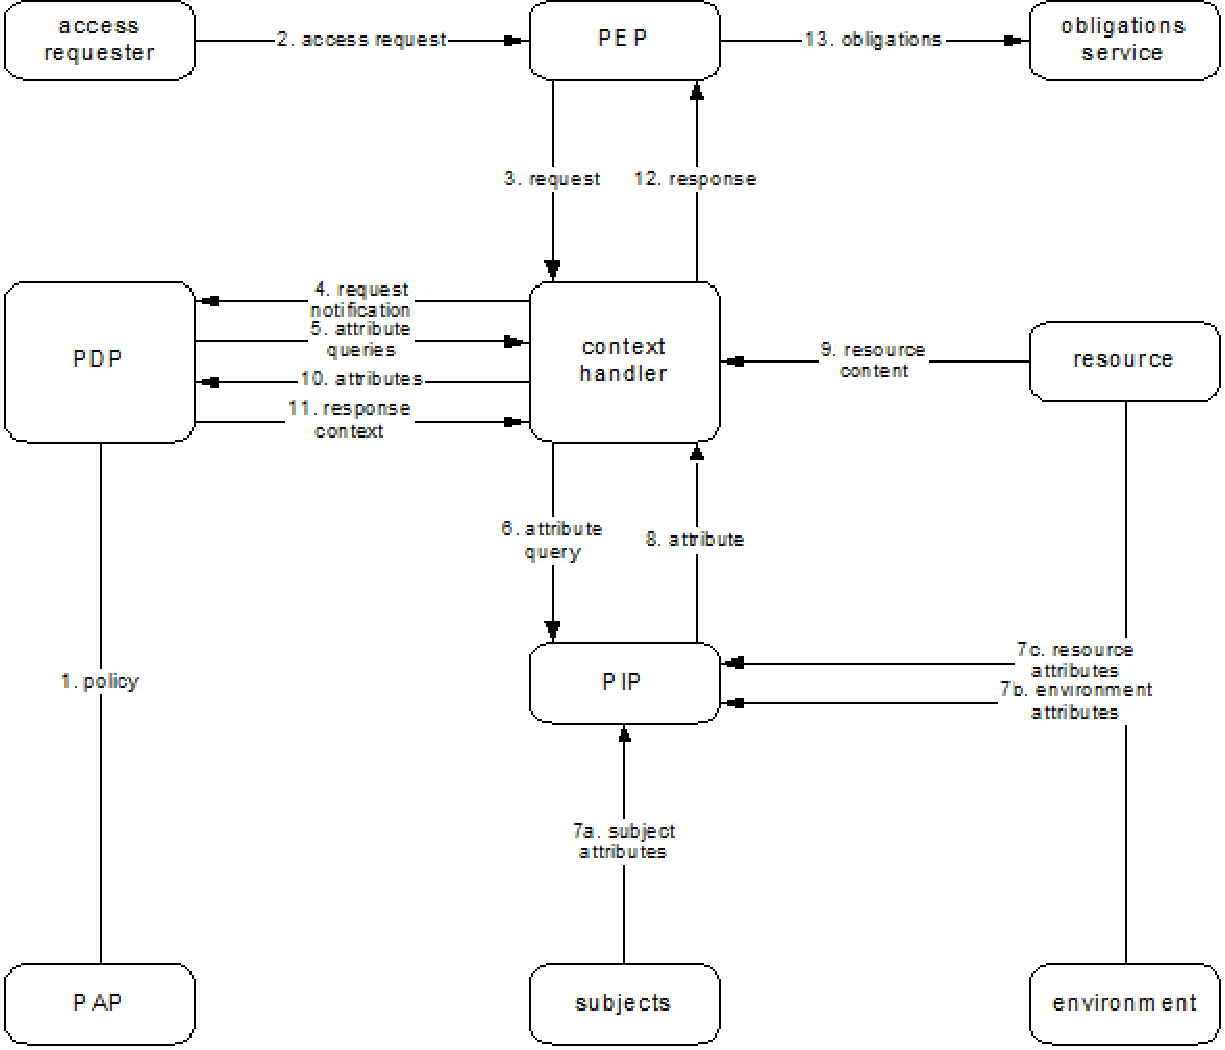
\includegraphics[scale=0.68]{it_sicherheitsmanagement/xacml.pdf}

Quelle: \url{http://docs.oasis-open.org/xacml/3.0/xacml-3.0-core-spec-os-en_files/image002.gif}



\section{IDM1 - Organisationsinternes Identitäts- und Zugriffsmanagement}
Zentrale Fragestellung: Wie können sehr viele Benutzer mit unterscheidlichen Funktionen effizient verwaltet werden?

\subsection{Identitätsspeicher}
\begin{itemize}
	\item Vorhalten digitaler Identitäten/Nutzerkonten
	\item Beispiele: HR-Systeme, Datenbanken, Verzeichnisdienste
	\item Anfragen basieren auf Eigenschaften (z.B. (L)DAP)
	\begin{itemize}
		\item \textit{Schema} bestimmt Struktur, Attribute und Matching Rules (Konsistenz wichtig!)
		\item Klassenhierarchie zur Beschreibung einer Person
	\end{itemize}
	\item Struktur Verzeichnisdienst: Hierarchisch
\end{itemize}


\subsection{Organisationsinterne Integration}

\subsubsection{Grundlegende Fragestellungen}
\begin{itemize}
	\item Identifikation der Datenquellen
	\item Datenautorität: Wem gehören die Daten?
	\item Datenaggregation: Wie werden die einer digitalen Identität zugehörigen Daten erkannt?
	\item Datenaktualität: Wie erfolgt der Abgleich?
	\item Datenkonsument: Wer benötigt welche Daten?
	\item Datenschutz
	\item Zentral vs. Dezentral und Homogenität vs. Heterogenität
\end{itemize}

\subsubsection{Bewertung zentraler Verzeichnisdienst}
\begin{itemize}
	\item Vorteile: Keine {Redundanz, komplexe Synchronisation, Inkosistenz}, Konzentration der Sicherheitsmaßnahmen an einer Stelle
	\item Nachteile: Legacy Systeme, Verlust der Autarkie, Single Point of Failure, Aggregation aller Benutzerdaten an einer Stelle (Angriffsziel)
\end{itemize}

\subsubsection{Virtual Directory}
\begin{itemize}
	\item Middleware zur dynamischen Aggregation verteilter Identitätsdaten
	\item Vorteile: Keine Redundanz, Nutzung lokaler Authentifikationsmechanismen (Pass-through Authentication)
	\item Nachteile: Verfügbarkeit zur Laufzeit nicht garantiert, keine Synchronisationsfunktionalität
\end{itemize}

\subsubsection{Meta Directory}
\begin{itemize}
	\item Synchronisation verteilter Identitätsdaten mit aggregiertem Verzeichnisdienst (vorgeschaltet)
	\item Vorteile: Sehr gute Suchperformance, Nachverfolgbarkeit von Datenflüssen
	\item Nachteile: Synchronisationsverzögerungen, zusätzliches, zentrales Berechtigungsmanagement, alle Daten zentral $\rightarrow$ Datenschutz?
\end{itemize}

\subsubsection{Provisioning System}
\begin{itemize}
	\item Anlegen, Pflege (Synchronisation), Entfernen verteilter Identitätsdaten
	\item Synchronisation verschiedener Attributwerte aus angebundenen Ressourcen nach vorgegebenen Regeln
	\item Integriertes Passwort-Management
	\item Vorteile: Self Service, Nachverfolgbarkeit von Datenflüssen
	\item Nachteile: Keine zentrale, aggregierte Sicht
\end{itemize}



\section{IDM2 - Föderatives IAM}

\subsection{Domänen-übergreifendes Identitäts- und Zugriffsmanagement}

\subsubsection{Einordnung Authentifikations- und Autorisierungsinfrastruktur (AAI)}
\begin{itemize}
	\item Auslagerung von Authentifikation und Autorisation in Infrastrukturdienste
	\item Komplexitätsreduktion (z.B. SSO)
	\item Domänenübergreifender Autausch von Identitätsdaten
	\item Nur ein Login für alle Dienste und Ressourcen benötigt
\end{itemize}

\subsubsection{Organisationsübergreifende AAI}
\begin{itemize}
	\item Voraussetzungen: Vertrauensbeziehungen zwischen den Teilnehmern, Zusammenschluss zu Föderationen
	\item Standardisierung durch Security Assertion Markup Language (SAML)
\end{itemize}


\subsection{Ausgewählte Technologien}

\subsubsection{Kerberos V4: Interrealm-Authentifikation}
\begin{itemize}
	\item Realm ist "`Herrschaftsbereich"', verlangt Namensschema zur Unterscheidung der Realms
	\item Idee: KDC von Realm B agiert wie eine Ressource in Realm A $\rightarrow$ gemeinsames Geheimnis mit KDC von Realm A
	\item Problemstellung: Vielzahl von Zugangspunkten, an allen muss authentifiziert werden
\end{itemize}

\subsubsection{RADIUS}
\begin{itemize}
	\item Problemstellung: Vielzahl von Zugangspunkten, an jedem muss authentifiziert werden
	\item Hierarchische Struktur von RADIUS Servern der verschiedenen Organisationen
	\item RADIUS Server des Network Access Servers (NAS) dient als Proxy zum RADIUS Server der Heimatorganisation (z.B. Eduroam)
	\item Authentifizierung durch die Heimatorganisation, Autorisierung durch die Zielorganisation
	\item Client und Server besitzen ein vorab vereinbartes, gemeinsames Geheimnis
	\item RADIUS verwendet keine Nachrichtenverschlüsselung
\end{itemize}

\subsubsection{SAML}
\begin{itemize}
	\item Austausch von Authentifizierungs- und Autorisierungsinformationen über institutionelle Grenzen hinweg
	\item XML basiert, OASIS Standard
	\item Bietet Profile für einige Use-cases, ist aber zusäzlich erweiterbar
	\item \textbf{Definitionen}
	\begin{itemize}
		\item Principal/Subjet: Subjekt, das Zugriff auf geschützte Ressource erhalten will
		\item Asserting Party/Identify Provider: Bietet Authentifikation von Principals
		\item Relying Party/Service Provider: Bietet Zugriff auf geschützte Ressourcen, benötigt identitätsbezogene Informationen für Autorisierungsentscheidung
	\end{itemize}
	\item \textbf{Bestandteile}
	\begin{itemize}
		\item Profiles: Definiert einen Use-case auf Basis von \textit{Bindings}, \textit{Protocols} und \textit{Assertions}
		\item Binding: Bildet SAML Protokoll auf Nachrichten- und Kommunikationsprotokolle ab
		\item Protocols: Protokolle zum Autausch von Assertions
		\item Assertions: Authentifizierungsinformationen, Attribute und Autorisierungsmerkmale
	\end{itemize}
	\item Beispielprofile: Web Browser SSO Profile, ECP Profile (SSO für nicht-browser Anwendungen), Single Logout Profile
\end{itemize}

\subsubsection{WebSSO - Ablauf}
\begin{enumerate}
	\item Weiterleitung zum Discovery Service und Auswahl des Identity Providers (optional)
	\item Weiterleitung zum IdP
	\item Authentifikation durch den IdP: Übergabe einer Assertion mit Authentication Statement und Attribute Statement
	\item Weiterleitung zum Service Provider und Übergabe der Assertion
\end{enumerate}
Bindings: HTTP-Redirect, HTTP Post

\subsubsection{SAML in der Praxis: Shibboleth}
\begin{itemize}
	\item OpenSource (Apache License)
	\item Attribute Based Access Control
	\item Ermöglicht föderatives Identitätsmanagement
	\item Einstz beispielsweise bei Elsevier, Asknet, Gigamove
	\item \textbf{Ablauf am Beispiel Gigamove}
	\begin{enumerate}
		\item Aufruf der Gigamove Webseite der RWTH Aachen
		\item Weiterleitung zum DFN, Heimateinrichtung auswählen
		\item Weiterleitung zum Shibboleth Provider des KIT
		\item Weiterleitung "`zurück"' zur Gigamove-Webseite der RWTH Aachen
	\end{enumerate}
\end{itemize}

\subsubsection{Zugang über einen SSH-Server}
Es existieren drei Varianten.
\begin{enumerate}
	\item \textbf{Variabte 1 - Enhanced Proxy}
	\begin{itemize}
		\item Delegation der Autorisierungsentscheidung über PAM
		\item Vorteil: Kein spezieller SSH-Client nötig
		\item Nachteil: Password wird im Klartext an den Service Provider übertragen
	\end{itemize}
	\item \textbf{Variabte 2 - Enhanced Client}
	\begin{itemize}
		\item PAM dient lediglich als Schnittstelle zum SAML-SP
		\item SSH-Client fungiert als Enhanced Client
		\item Vorteil: Service Provider erhält keine Kenntnis des Passworts
		\item Nachteil: Modifizierter SSH-Client nötig
	\end{itemize}
	\item \textbf{Variabte 3 - Public Key based Authentication}
	\begin{itemize}
		\item Authentifizierung gegen Service Provider
		\item Autorisierung basiert auf aktuellen Attributen des Identity Providers
		\item PAM beauftragt SAML-SP eine AttributeQuery durchzuführen
	\end{itemize}
\end{enumerate}

\subsubsection{Metadatenverwaltung der Föderation}
\begin{itemize}
	\item Es muss sichergestellt werden, dass alle Föderationsmitglieder sich gegenseitig authentifizieren können $\rightarrow$ Metadaten zur Definition der Föderation notwendig
	\item Metadaten können zentral in einem Dokument verwaltet werden, enthalten Zertifikate der SPs und IdPs und enthalten Adressen der unterstützten Kommunikationsschnittstellen der Teilnehmer
\end{itemize}


\subsection{Föderatives Identitätsmanagement im Web 2.0}

\subsubsection{OAuth 1.0}
\begin{itemize}
	\item Anwendungsfall: Benuter (User) kann einer Anwendung (Consumer) Zugriff auf Daten erlauben, die von einer anderen Anwendung verwaltet werden (Service Provider)
	\item \textbf{Ablauf}
	\begin{enumerate}
		\item User stellt Anfrage an den Consumer
		\item Consumer beantragt ein Abfrage-Token beim Service-Provider
		\item User wird zum Service Provider weitergeleitet
		\item User gibt seine Daten und bestätigt die Anfrage des Consumers
		\item Consumer erhält Zugangs-Token
		\item Consumer kann auf die geschützten Ressourcen zugreifen
	\end{enumerate}
\end{itemize}

\subsubsection{OAuth 2.0}
\begin{itemize}
	\item Weiterentwicklung von OAuth 1.0, allerdings nicht rückwärtskompatibel
	\item Fokus auf Komplexitätsreduktion für den Client(-entwickler)
\end{itemize}

\subsubsection{OpenID}
\begin{itemize}
	\item \textbf{Ablauf}
	\begin{enumerate}
		\item Nutzer gibt seine OpenID-URL an
		\item SP lädt diese URL herunter, darin enthalten: Verweis auf den IdP
		\item Optional: RP handelt mit IdP (per Diffie-Hellman) einen gemeinsamen Schlüssel aus
		\item SP schickt einen HTTP-Redirect auf den IdP an den Nutzer
		\item Nutzer authentifiziert sich beim IdP
		\item IdP schickt HTTP-Redirect an den SP mit Aussage über die Authentifizierung
		\item SP prüft die Aussage. Falls DH-Schlüssel vorhanden hiermit, anderenfalls durch Nachfrage
	\end{enumerate}
	\item Bewertung: Massive Verbreitung, allerdings keine Verschlüsselung gefordert, Nutzer kann eine beliebige Id angeben, die gemäß Verfahren heruntergeladen werden muss
\end{itemize}


\subsection{Zusammenfassung}
\begin{itemize}
	\item Föderatives Identitätsmanagement erlaubt einen organisationsübergreifenden Austausch von Identitätsinformationen
	\item Vorteile: Aktualität, SSO, viele Registrierungsprozesse entfallen
	\item Allerdings organisationsübergreifendes Vertrauen notwendig
\end{itemize}



\section{Business Continuity Management}

\subsection{Motivation}
\begin{itemize}
	\item Unternehmen sind abhängig von Einrichtungen, Rechnern, Diensten, Personal, Daten, Kommunikationsverbindungen, etc.
	\item Was passiert, wenn diese Ressourcen im Krisenfall ausfallen?
\end{itemize}


\subsection{Was ist Business Continuity Management}
"`Ganzheitlicher Managementprozess zur Fortführung der kritischen Geschäftsprozesse bei Eintritt eines Notfalls."'\footnote{BSI-Standard 100-4, S. 100}

\subsubsection{Notfallmanagement nach BSI 100-4}
\begin{enumerate}
	\item Initiierung durch das Management mit Zieldefinition und Organisation der Verantwortlichkeiten und des Krisenstabs
	\item Konzeptions des Notfallvorsorgekonzepts mit \textit{Business Impact Analyse} (Priorisierung der Geschäftsprozesse für den Krisenfalls), Risikoanalyse und der Erstellung eines Notfallhandbuchs
	\item Umsetzung des Notfallvorsorgekonzepts: Kosten- und Aufwandschätzung, Umsetzung der Maßnahmen, Sensibilisierung und Schulung
	\item \textbf{Notfallbewältigung}
	\begin{enumerate}
		\item Meldung bei zentraler Meldestelle
		\item Eskalation durch Krisenstabsleiter. Störung/Notfall/Krise?
		\item Sofortmaßnahmen einleiten
		\item Notfall bewältigen: Do-Plan-Check-Act
	\end{enumerate}
	\item Tests und Übungen: Tests der wesentlichen Bestandteile, Angemessen beachten
	\item Aufrechterhaltung und Verbesserungen: Regelmäßige Bewertung des Notfallmanagements
\end{enumerate}
Iterativer Prozess, daher im Anschluss ein Sprung zu (2).

\subsubsection{Business Impact Analyse}
\begin{enumerate}
	\item Auswahl einzubeziehender Organisationseinheiten und Prozesse
	\item Schadensanalyse
	\item Festlegung Wiederanlaufparameter
	\item Priorisierung der Geschäftsprozesse
	\item Abschätzung des Ressourcenbedarfs
	\item Priorisierung der Ressourcen
\end{enumerate}

\subsubsection{Notfallhandbuch}
Das Notfallhandbuch besteht üblicherweise aus folgenden Teilen:
\begin{itemize}
	\item Sofortmaßnahmen
	\item Krisenstabsleitfaden
	\item Krisenkommunikationsplan
	\item Geschäftsfortführungsplan
	\item Wiederanlaufplan
\end{itemize}


\subsection{Vorfallbehandlung}

\subsubsection{Computer Emergency Response Team (CERT)}
\begin{itemize}
	\item Lösung konkreter Sicherheitsvorfälle
	\item Warnungen vor Sicherheitslücken mit Lösungsansätzen
	\item Verschiedene CERTs, die verschiedenen Einrichtungen zugeordnet sind (z.B. Bund oder KIT)
\end{itemize}



\section{Secure Data Outsourcing}

\subsubsection{Generelle Vorteile}
\begin{itemize}
	\item Kosten sparen
	\item Höhere Verfügbarkeit/Robustheit
	\item Vereinfachte Administration
	\item Nachteil: Mangelnde Datenvertraulichkeit. Naheliegend: Verschlüsselung, lässt allerdings dann auch keine Datenverarbeitung vor Ort zu (Anbieter ist "`Honest, but curious"')
\end{itemize}


\subsection{Existierende Ansätze}

\subsubsection{Cryptografische Maßnahmen}
\begin{itemize}
	\item Deterministische Verschlüsselung: Ermittlung einzelner Chiffrate ohne Schlüssel schwierig, allerdings sind Chiffrate unterscheidbar
	\item Probabilistische Verschlüsselung: Chiffrate weder lesebar noch unterscheidbar. Jedoch keine Anfragen möglich
	\item Homomorphe Verschlüsselung: $Enc(k_1) \oplus Enc(k_2) = Enc(k_1 \otimes k_2)$. Ermöglicht Aggregation von Attributwerten, allerdings hoher Rechenaufwand und keine SELECT-Anfragen möglich
\end{itemize}

\subsubsection{Data Partitioning}
\begin{itemize}
	\item Aufteilung der Daten auf verschiedene Storage Provider $\rightarrow$ Unkenntlichkeit von Zusammenhängen zwischen Attributen
	\item Nachteil: Mehrere Storage Provider notwendig; ggf. zu wenige vorhanden
\end{itemize}

\subsubsection{k-Anonymisierung}
Jede mögliche Belegung eines Identifikators muss entweder nicht oder mindestens k-mal im Datensatz vorkommen. Operationen zur Sicherstellung: Suppresion (*), Generalization (M*) oder Einfügen falsche Einträge.


\subsection{Aktuelle Forschung: Securus}
Anwendungsfall: Datenbank mit Patientendaten.

\subsubsection{Von Securus adressierte Schutzziele}
\begin{itemize}
	\item Vertraulichkeit: Sicherstellung der Vertraulichkeit von Daten, die bei externen Providern abgelegt werden
	\item Datenschutz: Datenschutzrechtliche Vorgeben werden wahrgenommen und erfüllt
	\item Verfügbarkeit: Auslagern von Daten ermöglicht eine Steigerung der Verfügbarkeit der Daten
\end{itemize}

\subsubsection{Workflow}
\begin{enumerate}
	\item Benutzerseite: Definition des \textit{Policy Profile} über \textit{Securus Latin} (domänenspezifische Sprache)
	\item Securus: Tranformiere \textit{Policy Profile} in den \textit{Mediator}
	\item Mediator: \textit{Mediator} übernimmt die Verwaltung der Storage Provider und leitet alle Anfragen weiter
\end{enumerate}

\subsubsection{Access Policies} 
Access Policies spezifizieren eine Menge von Anfragen, die effizient auf den Daten ausführbar sein sollen.

\subsubsection{Confidential Constraits (CCs)}
Eine Untermenge an Attributen, deren Kombination als vertraulich gilt.

\subsubsection{Inference Constraits (ICs)}
Es wird angenommen, dass Angreifer kein Wissen aus deterministischen Chiffraten des entsprechenden Attributs gewinnen können.

\subsubsection{Securus-PT: Transformation des Policy Profiles}
\begin{enumerate}
	\item Verschlüssele jeden Wert der \textit{data table}. Einträge können per Id abgerufen werden, es können jedoch keine Anfragen ausgeführt werden
	\item Erstelle \textit{index table} für jede Access Policy. Ermöglicht effiziente Ausführung von entsprechenden Anfragen, die Attribute/Kombinationen aus Attributen werden per Id angesprochen
	\item \textbf{Substitutionsklassen}
	\begin{itemize}
		\item Idee: Klassifikation der Sicherheitsmechanismen anhand der Art, wie Attributwerte beim Storage Provider vorliegen
		\item Confidential Constraits und Access Policies schränken die Möglichkeiten ein, Substitutionsklassen zu wählen $\rightarrow$ Lösung als Integer Linear Programming von einem ILP-Server
		\item Beispiel: Mitarbeiterdatenbank, verteilt auf zwei Storage Provider. Name, DoB und Salary
		\begin{enumerate}
			\item Verschlüssele jeden Wert der \textit{data table}
			\item Erstelle \textit{index table} für jede Access Policy: Effiziente Abfragen möglich. Alle \textit{index tables} werden bei allen Storage Providern angelegt, bleiben allerdings ggf. leer
			\item Fülle \textit{index tables}, so dass alle ICs und CCs erfüllt sind mit (un-)verschlüsselten Werten
		\end{enumerate}
	\end{itemize}
\end{enumerate}

\subsubsection{Zusammenfassung Securus}
\begin{itemize}
	\item \textbf{Konzept}
	\begin{itemize}
		\item Herausforderung für sicheres Data Outsourcing: Matching von Datenvertraulichkeits- und Datenanfragbarkeitsanforderungen
		\item Securus automatisiert diesen Prozess
	\end{itemize}
	\item \textbf{Benutzung}
	\begin{enumerate}
		\item Definition von Access Policies und Confidential Constraits mit Securus-Latin
		\item Nutzung von generierten Mediatoren zur Ablage und Abfrage von Daten
	\end{enumerate}
	\item \textbf{Funktionsweise}
	\begin{itemize}
		\item Securus transformiert Policies in ein ILP-Problem
		\item Die eingesetzten Sicherheitsmechanismen werden dann entsprechend gewählt
	\end{itemize}
\end{itemize}



\section{Secure Data Sharing}

\subsection{Problemstellung}
\begin{itemize}
	\item Vorteile: Verfügbarkeit, Bandbreite, vereinfachte Administration
	\item Im Gegensatz zu \textit{Data Outsourcing} ist Teilen der Daten explizite Anforderung
	\item Nachteil: Vertraulichkeit und Integrität der Daten gefährdet
\end{itemize}

\subsubsection{Verschlüsselung der Daten}
\begin{itemize}
	\item Naiver Ansatz: Daten symmetrisch verschlüsseln und Datenschlüssel direkt an andere weitergeben. Nachteile: Entzug von Zugriffsrechten aufwendig, sicherer Kanal zur Schlüsselweitergabe nötig
	\item Besser: Austausch neuer Schlüssel durch Nutzung bereits ausgetauschter Schlüssel. Initialer Austausch von (a-)symmetrischen Schlüsseln notwendig
\end{itemize}


\subsection{Shared Cryptographic File Systems}
\begin{itemize}
	\item Vertraulicher Datenaustausch zwischen Benutzern über externe Speicheranbieter mit Ende-zu-Ende-Sicherheit
	\item Zusätzlich zur Sicherung der Integrität: Signaturen und/oder MACs
	\item Initialer Autausch nicht Teil des SCFS
\end{itemize}

\subsubsection{SiRiUS}
\begin{itemize}
	\item Stellt Vertraulichkeit und Integrität sicher: Nutzerdaten werden vor Ablage auf dem Dateiserver verschlüsselt und signiert
	\item Jeder Benutzer besitzt ein Schlüsselpaar
	\item Ein Besitzer für jeden Verzeichnisbaum
	\item Overlays zu bestehenden Dateisystemen
	\item Pro Datei ein symmetrischer Verschlüsselungskey und ein Keypair zur Signierung
	\item Lesezugriff durch Weitergabe des sym. Schlüssels und Schreibzugriff durch Weitergabe des privaten Schlüssels
	\item Sicherung der Metadaten: Besitzer der Datei signiert jede Änderung mit seinem privaten Schlüssel. Problem: Freshness nicht gewährleistet (Rollback-Angriff: Ehemals Schreibberechtigte können ältere md-Files hochladen, um Schreibberechtigung wieder zu erlangen. Gegenmaßnahmen: Gültigkeit der Signatur periosdisch auffrischen, resscourcenintensiv, Stichwort Hash-Tree)
	\item Beim Entzug von Leserechten: Sofortige Neuverschlüsselung
\end{itemize}

\subsubsection{Cepheus}
\begin{itemize}
	\item Stellt ebenfalls Vertraulichkeit und Integrität der Nutzerdaten sicher
	\item Führt zusätzliche Schlüssel für Benutzergruppen ein
	\item Keine Unterscheidung zwischen Lese- und Schreibrechten
	\item Sicherung der Integrität und Freshness der Metadaten über \textit{Merkle Hash Tree}
	\item Beim Entzug von Leseberechtigung: Lazy Revocation (Problem: Entzug erst nach Neuschreiben der Daten wirksam)
\end{itemize}

\subsubsection{Cryptree}
\begin{itemize}
	\item Ordnet jeder Datei/Verzeichnis einen Satz Schlüsseln zu
	\item Eigener \textit{Write Cryptree} für das Erteilen von Schreibrechten, Dateien werden zusätzlich signiert
	\item Setzt ebenfalls Lazy Revocation ein
\end{itemize}

\subsubsection{Shared Cryptographic File Systems: Risiko}
Tradeoff zwischen Verminderung des Risikos gegenüber Kosten/Ressourcenbedarf.


\subsection{Abstrakte Repräsentation: Schlüsselgraph}
\begin{itemize}
	\item Benutzer und deren bekannte Schlüssel bilden einen Schlüsselgraphen
	\item Erweiterung: Verschlüsselte Ressourcen
	\item Systeme für Secure Datasharing erzeugen implizit einen Schlüsselgraphen
	\item Ziel: Veringere Anzahl der Kanten
	\item Simpler Ansatz, abgeleitet aus Zugriffskontrollmatrix: Ein Schlüssel pro Benutzer und pro Ressource
	\item Mögliche Optimierung: Capability List, benötigt je nach Szenario weniger Kanten $\rightarrow$ welcher Ansatz ressourcenschonender ist, hängt vom Szenario ab
\end{itemize}


\subsection{Aktuelle Forschung: Abschätzen des Ressourcenbedarfs über Änderungen des Schlüsselgraphen}
\begin{itemize}
	\item Ziel: Abhängigkeit des Ressourcenbedarfs von konkretem Szenario und konkretem System für Secure Data Sharing finden
	\item Vorgehen: Modellierung des Systems als Regelsatz, der Änderungen am Schlüsselgraphen vornimmt, dann Ableitung des Ressourcenbedarfs aus den Änderungen am Schlüsselgraphen $\rightarrow$ Eingabe für Simulation: Workloads als Abfolge von Ereignissen (Erfassung realistischer Workloads schwierig)
\end{itemize}



\section{Anonymität}
\begin{itemize}
	\item ... kann Vertraulichkeit "`ersetzen"'
	\item ... kann Datenschutz ermöglichen
	\item ... kann Voraussetzung für ein technisches System sein
	\item ... kann vor Repressalien schützen, bietet aber auch Missbrauchspotential
\end{itemize}

\subsubsection{Definition nach BSI:}
Die Identität einer oder mehrerer an einem anonymen Vorgang beteiligter Instanzen ist nicht bestimmbar, weil sie entweder
\begin{itemize}
	\item den anderen beteiligten Instanzen nicht bekannt ist (Nichtbewusstsein),
	\item gegenüber den anderen beteiligten Instanzen nicht in Erscheinung tritt (Nichtgenanntsein) \\ oder
	\item innerhalb des anonymen Vorgangs ohne erkannbaren Namen agiert (Namenlosigkeit).
\end{itemize}
\footnote{\url{https://www.bsi.bund.de/DE/Publikationen/Studien/anonym/wasistanonymitaet.html}}

Problem: Identität mit hinreichend großem Aufwand eben doch bestimmbar, besonders im IT-Umfeld.

\subsubsection{Anwendungsfelder}
\begin{itemize}
	\item Anonymisierung von Daten
	\item Anonyme Kommunikation (Schwerpunkt in dieser Vorlesung)
\end{itemize}

\subsubsection{Pseudonymisierung}
\begin{itemize}
	\item Erlaubt eine digitale Identität zu verwenden ohne seine reale Identität preiszugeben. Enscheidung, welche Informationen er über sich herausgiebt, liegt beim Subjekt selbst
\end{itemize}

\subsubsection{Anynome Kommunikationsstufen}
Eigenschaften anonymer Kommunikation: Sender- und Empfängeranonymität.
\begin{enumerate}
	\item Absolute anonymity: Beobachter kann nicht feststellen, ob eine Nachricht verschickt wurde.
	\item Beyond suspicion: Beobachter kann nicht feststellen, von wem die Nachricht verschickt wurde
	\item Probable innocence: Für den Beobachter ist es wahrscheinlicher, dass die Nachricht nicht vom Sender kommt, als dass die von ihm kommt
	\item Possible innocence: Für Beobachter exisitiert Wahrscheinlichkeit, dass die Nachricht nicht vom Sender kommt
	\item Exposed: Beobachter kann Sender identifizieren, aber gegenüber Dritten nicht beweisen, dass der Sender sie wirklich gesendt hat
	\item Provably exposed: Verbindlichkeit ist gegeben
\end{enumerate}

\subsubsection{Anonymität im Internet}
\begin{itemize}
	\item Szenario: Anonymes Senden von Nachrichten über (vertrauenswürdigen) Proxy
	\item Erweiterung: Einführen mehrerer Proxies in Reihe (Mix-Kaskaden). Problem: Mögliche Kollaboration zwischen Mixes $\rightarrow$ Mixes dynamisch wählen
	\item \textbf{Onion Routing}
	\begin{itemize}
		\item Dynamische Wahl der Mixes, Benutzer können eigenen Endknoten als Mix anbieten und mischen eigenen Traffic und den Traffic der anderer Knoten.
		\item Mögliches Problem, Sybil-Attacke: Beobachten von Kommunikationsmuster im Netz
		\item Implementierungen: Tor, Freenet, I2P
	\end{itemize}
\end{itemize}



\section{Peer-to-Peer und Online Social Networks}

\subsection{Methodik für empirische OSN-Studien}
\begin{itemize}
	\item Datenschutzkonforme und Privatsphäre-wahrende Analyse: Analyse vollständig zur Laufzeit des Analyse-Systems, ledigliches Speichern statistischer (anonymisierter) Daten
	\item Breitensuche: Analysiere mind. ein Profil und davon ausgehend alle Freunde, etc.
	\item Tiefensuche: Analysiere ein Seed-Profil, dann einen Freund, dann einen Freund des Freunde, etc.
\end{itemize}


\subsection{Online Social Networks}
\begin{itemize}
	\item Attribut-Verfügbarkeit. Mögliche Gefahr: Wenn diverse OSN-Profile eines Nutzer in Verbindung gebracht werden, kann ein umfassendes digitales Abbild der Person erstellt werden (Freundeslisten zu ca. 50\% öffentlich verfübar)
	\item Profil-Verknüpfbarkeit (Linkability)
	\item \textbf{Attribut-Vorhersagbarkeit (Attribute Prediction)}
	\begin{itemize}
		\item Freundeslisten in ca. 50\% der Profile öffentlich
		\item >78\% teilen mindestens ein Attribut öffentlich, dass sie auch verstecken könnten
		\item Hohe Genauigkeit bei Attribut-Vorhersagen
	\end{itemize}
\end{itemize}


\subsection{Zusammenfassung}
\begin{itemize}
	\item \textbf{Attributverfügbarkeit}
	\begin{itemize}
		\item Viele Attribute noch immer öffentlich verfügbar
		\item Alt-Profile oft noch online
		\item Ca. die Hälfte der Freundeslisten öffentlich
	\end{itemize}
	\item \textbf{Quantifizierte Risiken}
	\begin{itemize}
		\item Linkability: Vier überlappende Freunde oft ausreichend für Linking
		\item \textbf{Attribute Prediction}
		\begin{itemize}
			\item Location-Attribute und Alter kann predeziert werden (mit Ungenauigkeit)
			\item Andere Attribute schwerer zu prezidieren, wenn kein komplexer Algorithmus oder zusätzliche Informationen hinzugezogen werden
		\end{itemize}
	\end{itemize}
\end{itemize}

\chapter{Programmierparadigmen}

Zusammenfassung der Vorlesung "`Programmierparadigmen"' aus dem Wintersemester 2014.\footnote{\url{https://pp.info.uni-karlsruhe.de/lehre/WS201415/paradigmen/}}

\section{Funktionale Programmierung}

\subsection{Rekursion}
\begin{itemize}
	\item Auswertung: Zwischenausdrücke können mit Eingabegröße wachsen
	\item Speicherverbrauch in \(\mathcal{O}(n)\) bei \(\mathcal{O}(n)\) Aufrufen
	\item \textbf{Akkumulation}
	\begin{itemize}
		\item Übergebe Zwischenergebnisse in Hilfsparameter \texttt{acc}
		\item Speicherverbrauch in \(\mathcal{O}(1)\) bei \(\mathcal{O}(n)\) Aufrufen
	\end{itemize}
\end{itemize}

\subsubsection{Endrekursion}
\begin{itemize}
	\item Linearität: Eine Funktion heißt \textit{linear rekursiv}, wenn in jedem Defitionszweig nur ein rekursiver Aufruf vorkommt.
	\item Endrekursion: Eine linear rekursive Funktion heißt \textit{endrekursiv}, wenn in jedem Zweig der rekursive Aufruf nicht in andere Aufrufe eingebettet ist.
\end{itemize}


\subsection{Listen}
\begin{itemize}
	\item Eine Liste \texttt{(x:xs)} besteht immer aus Listenkopf \texttt{x} und Listenrest \texttt{xs}
\end{itemize}

\subsubsection{Pattern Matching}
\begin{itemize}
	\item Mehrere Gleichungen zur Definition einer Funktion
	\item Jede Gleichung gilt für Argumente mit speziellem Strukturmuster
	\item Überlappende Muster: Erste Gleichung wird angewandt
\end{itemize}


\subsection{Funktionen höherer Ordnung}

\subsubsection{Lambda-Notation}
\begin{itemize}
	\item Anonyme Funktionen und Funktionen höherer Ordnung möglich
	\item Beispiel: \(g(x,y)=x-\frac{y}{2} \longrightarrow\) \texttt{g = \textbackslash x y -> x - 2/y}
\end{itemize}

\subsubsection{Definition: Funktion höherer Ordnung}
Funktionen, die andere Funktionen als Parameter erhalten oder Funktionen als Rückgabewerte liefern, heißen Funktionen höherer Ordnung.

\subsubsection{Currying}
\begin{itemize}
	\item Ersetzung einer mehrstelligen Funktion durch Schachtelung einstelliger Funktionen.
	\item Jede Funktion erhält, wie oben erwähnt, nur ein Argument. Werden scheinbar mehrere Argumente definiert, so steckt immer Currying dahinter.
	\item Unterversorgung: Anwendung mehrstelliger Funktionen auf zu wenig Parameter
\end{itemize}

\textbf{Beispiel\footnote{\url{https://de.wikipedia.org/wiki/Currying\#Haskell}}}

\begin{lstlisting}[frame=single,numbers=left,mathescape,language=Haskell]
addiere x y = x + y
addiere 1 3                -- ist aequivalent zu (addiere 1) 3
addiereZu2  = addiere 2
addiereZu2 1               -- 3
\end{lstlisting}

\subsubsection{Namensbindung}
\begin{itemize}
	\item Bindungsstrukte legen Bedeutung und Geltungsbereiche von Variablen fest
	\item Verdeckung: Innere Bindungen verdecken äußere
	\item \textbf{Bindung}
	\begin{itemize}
		\item \texttt{f x = x*x}: Bindung von \texttt{x} im Rumpf von \texttt{f}, globale Bindung von \texttt{f}
		\item \texttt{\textbackslash x -> x*x}: Bindung von \texttt{x} innerhalb des \(\lambda\)-Ausdrucks
	\end{itemize}
\end{itemize}

\subsubsection{Lokale Bindung}
\begin{itemize}
	\item Anwendung: Lokale Hilfsfunktionen
	\item \texttt{let} bindet stärker als \texttt{where}
\end{itemize}

\textbf{Beispielse}

\begin{lstlisting}[frame=single,numbers=left,mathescape,language=Haskell]
energy m = let c = 299792458
           in m * c * c

energy m = m * c * c
  where c = 299792458
\end{lstlisting}

\subsection{Kombinatoren}

\subsubsection{Folds}
\begin{itemize}
	\item Anwendung einer Operation und eines Initialwertes auf eine Liste
	\item \textbf{Beispiel Summenberechnung}
	\begin{itemize}
		\item \texttt{sum = (+) 0}
		\item Berechnung mittels \texttt{foldr}: \texttt{(1 + (2 + (3 + (4 + 0))))} (rechts-geklammert)
		\item Berechnung mittels \texttt{foldl}: \texttt{((((1 + 0) + 2) + 3) + 4)} (links-geklammert)
	\end{itemize}
	\item Anwendung: Koplexe Funktionen als Kombination einfacher Funktionen
\end{itemize}

\subsubsection{Kombination von Listen}
\begin{itemize}
	\item Zusammenfügen von Listen per Reißverschluss: \texttt{zip = zipWith (,)}
	\item \texttt{zipWith} definiert eine Zusätzliche Operation
	\item Bricht ab, wenn eine der Listen keine weiteren Elemente enthält
\end{itemize}

\subsubsection{List Comprehensions}
\begin{itemize}
	\item Automatisiertes Erzeugen von Listen, basierend auf bereits existierenden Listen
	\item Inspiriert durch die mathematische Mengenschreibweise: \texttt{s = {[} 2 * x {|} x <- {[}0..{]}, x\textasciicircum 2 > 3 {]} } \footnote{\url{https://en.wikipedia.org/wiki/List_comprehension\#Haskell}}
	\item Multidimensionale Liste: \texttt{s = {[} 2*x*y {|} x <- {[}0..{]}, x\textasciicircum2 > 3, y <- {[}1,3..x{]}, y\textasciicircum2 < 100-x\textasciicircum2 {]}}
\end{itemize}


\subsection{Lazy Evaluation}

\subsubsection{Auswertung}
\begin{itemize}
	\item Struturierte Daten: Nur auswerten, falls wirklich benötigt wird
	\item Duplizierte Argumente: Auswertung maximal einmal (\textit{sharing})
	\item Pattern-Matching: So weit wie nötig, bis passendes Muster gematched
	\item Boolsche Operatoren: Auswertung bis zum ersten \textit{false} (\textit{short-circuit-Auswertung})
	\item \textbf{Nachteile}
	\begin{itemize}
		\item Erschwerte Fehlersuche
		\item Fehler, die beim Testen nicht beachten wurden, tauchen eventuell später im Betrieb auf
	\end{itemize}
\end{itemize}


\subsection{Typen}
\begin{itemize}
	\item Haskell ist statisch typisiert
	\item Jeder gültige Ausdruck hat immer einen Typ und wertet immer zu gültigen Werten dieses Typs aus
	\item Schreibweise: \texttt{e :: t} falls Ausdruck \texttt{e} und Typ \texttt{t}
	\item Untypisierbare Ausdrücke erzeugen Übersetzerfehler
	\item Haskell erkennt den korrekten Typ (fast immer) zuverlässig, optional manuelle Deklaration möglich
\end{itemize}

\subsubsection{Polymorphe Typen}
\begin{itemize}
	\item Der Listen-Typ sind polymorph, die Typvariable \texttt{{[}t{]}} steht auch für Nicht-Basistypen
	\item Typvariablen parametrisieren polymorphe Typen
	\item Typkonstruktoren wie \texttt{{[} {]}} erzeugen neue Typen aus bestehenden
	\item \textbf{Funktionstypen}
	\item Funktionstypen sind ebenfalls polymorph
\end{itemize}

\subsubsection{Beispiele}
\begin{itemize}
	\item Typen mehrstelliger Funktionen: \texttt{f x y = x * y, f :: Integer -> Integer -> Integer}
	\item Typen eingebauter Operatoren: \texttt{(<=) :: Integer -> Integer -> Bool}
	\item Tupel: \texttt{(3, True) :: (Integer, Bool); (not, 7) :: (Bool -> Bool, Integer)}
\end{itemize}

\subsubsection{Typinferenz}
Errechnen der Typen durch den Compiler, dadurch entstehen kompakte Programme, die trotzdem typsicher sind. Manuelle Deklaration ist dennoch möglich.

\subsubsection{Typsynonyme}
Ableiten neuer Typen aus vorhandenen. Z.B. \texttt{type String = {[}char{]}} (kann die Lesbarkeit erhöhen). Es werden keine explizit neuen Typen erzeugt.

\subsubsection{Typen bei der Fehlersuche}
\begin{itemize}
	\item Typendeklarationen können beim Lokalisieren von Programmfehlern helfen
	\item Beabsichtigten Typ der Funktion deklarieren
	\item \textbf{Beispiel}
	\begin{itemize}
		\item \texttt{isDigit :: Char -> Bool}\\\texttt{isDigit c = isIn c "0123456789"}
		\item \texttt{*Main> isDigit '3'} würde zu einem Typfehler führen
	\end{itemize}
\end{itemize}

\subsubsection{Mengen}
\begin{itemize}
	\item Mengen bestehen aus dem Typ \texttt{Set = ...} sowie Funktionen zum Iterieren, Einfügen, Löschen, Vergleichen, usw.
	\item Einfachste Implementierung als Listen: \texttt{type Set t = {[} {]}}
\end{itemize}


\subsection{Algebraische und rekursive Datentypen}

\subsubsection{Nachteile von Tupeln}
\begin{itemize}
	\item Produkttypen: Typen mit mehreren Komponenten. Beispiel: Personen mit Name und Alter \texttt{type Person = (String, Int)}
	\item Nachteil: Bedeutung von Werten nicht explizit; ungewollte Verwendung beliebiger \texttt{(String, Int)} Tupel
\end{itemize}

\subsubsection{Algebraische Datentypen}
\begin{itemize}
	\item Verwendung des Schlüsselwortes \texttt{data} statt \texttt{type} zur definition \textit{neuer} Typen
	\item Mehrere Konstruktoren möglich
\end{itemize}

\subsection{Anwendung algebraischer Datentypen}
\begin{itemize}
	\item \textbf{Algebraischer Datenstrukturen ermöglichen}
	\begin{itemize}
		\item Implementierung von Datenstrukturen
		\item Modellierung problemspezifischer Daten
	\end{itemize}
	\item \textbf{Einsatz von Pattern-Matching}
	\begin{itemize}
		\item Erleichtert Umsetzung komplexer Algorithmen
		\item Besonders für baumartige Strukturen
	\end{itemize}
	\item \textbf{Anwendungsbeispiele}
	\begin{itemize}
		\item Datenstrukturen: Maps, Bäume, Rot-Schwarz-Bäume
		\item Fehlerbehandlung
		\item Termersetzungssysteme
	\end{itemize}
\end{itemize}



\section{Theoretische Grundlagen}
Kalküle sind minimalistische Programmiersprachen zur Beschreibung von Berechnungen.	

\subsection{Der untypisierte $\lambda$-Kalkül (S159)}
\begin{itemize}
	\item Turing-mächtiges Modell funktionaler Programme zur Beschreibung sqeuentieller imperativer Konstrukte
	\item Linkassoziative Funktionsanwendung
	\item \(\lambda\)-Term: Ein Term der Form \texttt{(\(\lambda\)x.\(t_1\))\(t_2\)}
	\item \textbf{\(\alpha\)-Äquivalenz}
	\begin{itemize}
		\item \(t_1\) und \(t_2\) heißen \(\alpha\)-äquivalent, wenn \(t_1\) in \(t_2\) durch konsistente Umbenennung der \(\lambda\)-gebundenen Variablen überführt werden kann
		\item Funktionsbezeichnungen dürfen nicht geändert werden
		\item Beispiel: \texttt{\(\lambda\)x. (\(\lambda\)z. f(\(\lambda\)y. z y) x) = \(\lambda\)y. (\(\lambda\)x. f(\(\lambda\)z. x z) y)}
	\end{itemize}
	\item \textbf{\(\eta\)-Äquivalenz (S160)}
	\begin{itemize}
		\item Zwei Funktionen genau dann gleich sind, wenn sie für alle Argumente dasselbe Resultat liefern\footnote{\url{https://de.wikipedia.org/wiki/Lambda-Kalkül\#.CE.B7-Konversion}}
		\item Terme \texttt{\(\lambda\)x. f x} und \texttt{f} heißen \(\eta\)-äquivalent, falls \texttt{x} eine nicht-freie Variable von \texttt{f} ist
	\end{itemize}
\end{itemize}

\subsubsection{$\beta$-Reduktion}
\begin{itemize}
	\item Formalisiert das Konzept der Funktionsanwendung
	\item Anwendung ausschlißelich von links nach rechts
	\item Eine \(\beta\)-Reduktion entspricht der Ausführung der Funktionsanwendung auf einem Redex: \texttt{(\(\lambda\)x.\(t_1\))\(t_2 \Rightarrow\) \(t_1\){[} x \(\mapsto t_2\) {]}}
	\item Volle \(\beta\)-Reduktion: Jeder Redex kann reduziert werden
	\item \textbf{Beispiele}
	\begin{itemize}
		\item \texttt{(\(\lambda\)x.x)y \(\Rightarrow\) x{[} x \(\mapsto\) y {]} = y}
		\item \texttt{(\(\lambda\)x.x (\(\lambda\)x.x))(y z) \(\Rightarrow\) (x (\(\lambda\)x.x)){[} x \(\mapsto\) y z {]} = (y z)(\(\lambda\)x.x)}
	\end{itemize}
	\item \textbf{Kodierung mit Funktionen höherer Ordnung}
	\begin{itemize}
		\item Man braucht nicht unbedingt primitive Operationen
		\item Beispiel: \texttt{let}
		\item \texttt{let x = \(t_1\) in \(t_2\)} wird zu \texttt{(\(\lambda\)x.\(t_2\)) \(t_1\))}
		\item \texttt{let x = g y in f x = (\(\lambda\)x.f x)(g y) \(\Rightarrow\) f(g y)}
	\end{itemize}
\end{itemize}

\subsubsection{Kodierung natürlich Zahlen (Church-Zahlen)}
\begin{itemize}
	\item Einbettung von Daten und Operationen in den \(\lambda\)-Kalkül
	\item Eine (natürliche) Zahl drückt aus, wie oft die Funktion \texttt{s} angewendet wird
	\item \textbf{Church-Zahlen}
	\begin{itemize}
		\item \texttt{\(c_0\) = \(\lambda\)s. \(\lambda\)z. z}
		\item \texttt{\(c_1\) = \(\lambda\)s. \(\lambda\)z. s z}
		\item \texttt{\(c_2\) = \(\lambda\)s. \(\lambda\)z. s (s z)}
		\item \texttt{\(c_3\) = \(\lambda\)s. \(\lambda\)z. s (s (s z))} \\ \(\vdots\)
		\item \texttt{\(c_n\) = \(\lambda\)s. \(\lambda\)z. \(s^n\) z}
	\end{itemize}
\end{itemize}

\subsubsection{Rechnen mit Church-Zahlen}
\begin{itemize}
		\item Nachfolgerfunktion: \texttt{succ = \(\lambda\)n. \(\lambda\)s. \(\lambda\)z. s(n s z)} errechnet den Nachfolger. Beispielsweise ist \texttt{succ(\(c_2\)) = \(c_3\)}
		\item Addition: \texttt{plus = \(\lambda\)m. \(\lambda\)n. \(\lambda\)s. \(\lambda\)z. m s (n s z)}. Beispielsweise erreichnet \texttt{plus \(c_2\) \(c_3\) = \(c_5\)}
		\item Multiplikation: \texttt{times = \(\lambda\)m. \(\lambda\)n. \(\lambda\)s. n (m s)}.
		\item Potenzieren: \texttt{exp = \(\lambda\)m. \(\lambda\)n. n m}. Berechnung per Induktion über \texttt{n}
\end{itemize}

\subsubsection{Kodierung boolscher Werte}
\begin{itemize}
	\item \texttt{True} und \texttt{False} wird zu \texttt{\(c_{true}\) = \(\lambda\)t. \(\lambda\)f. t} und \texttt{\(c_{false}\) = \(\lambda\)t. \(\lambda\)f. f}
	\item \texttt{if \_ then \_ else \_} wird zu \texttt{\(\lambda\)a. a}. Beispielsweise wird aus \texttt{if True then x else y}: \texttt{(\(\lambda\)a. a) (\(\lambda\)t. \(\lambda\)f. t) x y \(\Rightarrow\) (\(\lambda\)t. \(\lambda\)f. t) x y \(\Rightarrow\) (\(\lambda\)f. x) y}
	\item \texttt{\(b_1\) \&\& \(b_2\)} wird zu \texttt{if \(b_1\) then \(b_2\) else False}
	\item \texttt{True \&\& True} ergibt: \texttt{\(\lambda\)a. a) \(c_{true}\) \(c_{true}\) (\(\lambda\)t. \(\lambda\)f. t)}
\end{itemize}

\subsubsection{Divergenz}
\begin{itemize}
	\item Terme, die nicht zu einer Normalform auswerten, divergieren
	\item Diese modellieren unendliche Ausführungen
\end{itemize}


\subsection{Typsysteme}
\begin{itemize}
	\item Typklassen definieren Funktionen, die für jede Instanz der Typklasse aufgerufen werden können
	\item Man kann eine Instanz für jeden Typ erstellen, indem man die Funktionen der Typklasse für den jeweiligen Typ definiert
	\item Beispiel: Vergleichsoperator (\texttt{==})
\end{itemize}

\subsubsection{Typen}
\begin{itemize}
	\item \textbf{Typen} legen die möglichen Werte von Variablen, Operationen und Operanden fest. Beispiel: Integer, Float, String
	\item \textbf{Statisch typisierte Sprachen:} Jede Variable/jeder Ausdruck hat einen vom Compiler bestimmbaren Typ. Beispiel: Java, Haskell, C++
	\item \textbf{Dynamisch typisierte Sprachen:} Typ von Variablen kann sich zur Laufzeit ändern. Beispiele: JavaScript, Python, PHP
\end{itemize}

\subsubsection{Typherleitung (F196)}
\begin{itemize}
	\item Nachweis von Herleitbarkeit als Herleitungsbaum
	\item Die Struktur des Herleitungsbaums wird durch den \(\lambda\)-Term bestimmt
	\item Zu jedem Subterm genau eine passende Regel: \texttt{App, Var, Abs oder Const}
	\item \texttt{t} ist typisierbar im Kontext \(\Gamma\), falls \(\tau\) mit \(\Gamma\vdash t_2~:~\tau_2\) exisitiert
	\item Beispiel auf Folie 196
\end{itemize}

\subsubsection{Untypisierbare \(\lambda\)-Terme (F197)}
\begin{itemize}
	\item Nicht alle sicheren Programme sind typisierbar \(\rightarrow\) Typsystem nicht vollständig bzgl. \(\beta\)-Reduktion
	\item Beispiel: \texttt{(\(\lambda\)x. x + 42) true} ist nicht typisierbar
	\item Die Korrektheit des Typsystems ist per Induktion über die Typsystemregeln beweisbar (F198)
\end{itemize}


\subsection{Polymorphie (F199)}
\begin{itemize}
	\item Polymorphe Funktionen: Verhalten hängt nicht vom konkreten Typ \(\tau\) der Elemente ab und haben unendlich viele Typen
	\item Beispiel: Operationen auf Containern (Zusammenfügen von Listen)
\end{itemize}

\subsubsection{\texttt{let}-Polymorphismus}
\begin{itemize}
	\item Beispielprogramm P: \texttt{let f = \(\lambda\)x. 2 in f(f true)}
	\item \texttt{f} ist eine polymorphe Hilfsfunktion: Anwendung erst auf \texttt{true}, dann auf \texttt{2}
	\item Kodierung: \texttt{let x = \(t_1\) in \(t_2\)} als neues Konstrukt im \(\lambda\)-Kalkül. Neue Typregeln mit \textit{Typschemata}
	\item \textbf{Typschemata (F202)}
	\begin{itemize}
		\item Ein Typ der Gestalt \(\forall\alpha_1.\forall\alpha_2.~...~\forall\alpha_n.~\tau\) heißt Typschema
		\item Es bindet freie Typvariablen \(alpha_1,...,\alpha_n\) in \(\tau\)
		\item Beispiel: \(\forall\alpha.~\alpha\rightarrow\alpha\) steht für unendlich viele Typen
	\end{itemize}
\end{itemize}


\section{Logische Programmierung}
Prolog-Programme bestehen aus einer Datenbasis, deren Einträge sich Fakten und Regeln nennen. Der Benutzer formuliert Anfragen an diese Datenbasis. Der Prolog-Interpreter benutzt die Fakten und Regeln, um systematisch eine Antwort zu finden. Ein positives Resultat bedeutet, dass die Anfrage logisch ableitbar ist. Ein negatives Resultat bedeutet nur, dass aufgrund der Datenbasis keine Ableitung gefunden werden kann.\footnote{\url{https://de.wikipedia.org/wiki/Prolog_(Programmiersprache)\#Grundprinzip}}

\subsection{Einführung in Prolog}
\begin{itemize}
	\item Situationsbeschreibung
	\item Definition von Objekten und Beziehungen zwischen Objekten
	\item Darstellbar als Terme einer freien Termalgebra
\end{itemize}

\subsubsection{Termsyntax}
\begin{itemize}
	\item Atome: z.B. \texttt{hans, inge, fritz, fisch}
	\item Zahlen: z.B. \texttt{3, 4.5}
	\item Variablen: z.B. \texttt{X, Y, \_X, X1, Fisch}
	\item Termlisten: z.B. \texttt{3, 4.5, X, fritz}
	\item Zusammengesetzt: z.B. \texttt{liebt(fritz,fisch), liebt(fritz,X)}
\end{itemize}

\subsubsection{Variablen}
Platzhalter für unbekannte Terme. Können auch "`Allgemeinheit"' ausdrücken, beispielsweise \texttt{liebt(X, fussball)} \(\rightarrow\) "`Alle lieben Fußball"'.

\subsubsection{Abfragen}
\begin{itemize}
	\item Alle Fakten werden zur Laufzeit in einer Datenbank gehalten
	\item Einleitung per \texttt{?}: z.B. \texttt{?liebt(fritz,fisch)}
	\item \textbf{Mehrfachlösungen}
	\begin{itemize}
		\item Durchsuche Datenbank von vorne nach hinten
		\item Versuche jeweils, Abfrageparameter mit Datenbankfaktor zu unifizieren
	\end{itemize}
	\item \textbf{Konjunktion von Abfragen}
	\begin{itemize}
		\item Konjunktion von Teilzielen getrennt durch Komma, entspricht logischem \(\wedge\)
		\item Erfülle Teilziele von links nach rechts und nehme jeweils erstes Ergebnis
		\item Mehrere Ergebnisse: Fahre mit dem ersten Ergebnis bis zum Ende fort, prüfe danach weitere Ergebnisse
		\item Nach Erfüllung eines Teilziels: Nächstes Teilziel erbt Instanziierung
	\end{itemize}
\end{itemize}

\subsubsection{Regeln}
\begin{itemize}
	\item Aufbau: Regelkopf (1 Term) und Regelrumpf (1+ Terme): \texttt{term :- termlist .}
	\item \texttt{:-} liest sich als \textit{wenn}, Kommata als \textit{und}
	\item \textbf{Beispiele}
	\begin{itemize}
		\item "`Wenn Inge X liebt und wenn X Fisch liebt, dann liebt Hugo X"':\newline\texttt{liebt(hugo,X) :- liebt(inge,X),liebt(X,fisch)}
		\item "`Wenn es jemanden gibt, der Fisch mag, dann liebt Emil Erna"':\newline\texttt{liebt(emil,erna) :- liebt(X,fisch)}
	\end{itemize}
\end{itemize}

\subsubsection{Logische Programmierung ist anders}
\begin{itemize}
	\item Keine herkömmlichen Variablen
	\item Prädikate liefern außer ihrer Erfüllbarkeit keinen Ergebniswert
	\item Aber Unifikation und Backtracking eingebaut
	\item Sehr gut geeignet für Such- und Constraintprobleme, weniger für Berechnungen
\end{itemize}


\subsection{Backtracking}
\begin{itemize}
	\item Visualisierung durch einen Ausführungsbaum
	\item Jedes Teilziel wird als Box mit vier Ein- bzw. Ausgängen dargestellt
\end{itemize}

\subsubsection{Der Algorithmus informell}
\begin{enumerate}
	\item Anlegen und erstmaliges Betreten der Box durch den \texttt{call}-Eingang beim ersten Aufruf des Teilziels
	\item Falls keine passende Regel gefunden wird, wird die Box durch den \texttt{fail}-Ausgang verlassen und gelöscht
	\item Für eine passende Regel werden Kind-Boxen für Teilziele im Regelrumpf angelegt. Die Box wird durch den \texttt{success}-Ausgang verlassen. Dieser verweist auf den \texttt{call}-Eingang der ersten Kindbox
	\item Falls keine Kinder existieren (Fakt), verweist \texttt{success} auf den \texttt{call}-Eingang des nächsten Teilziels
	\item Der \texttt{fail}-Ausgang verweist auf den \texttt{redo}-Eingang des vorherigen Teilziels
	\item Wird eine Box durch den \texttt{redo}-Eingang betreten, werden mit Hilfe des Choice Points weitere anwendbare Regeln gesucht. Falls kein Choice Point existiert, wird die Box durch \texttt{fail}
	\item Der \texttt{fail}-Ausgang der obersten/ersten Box erzeugt die Ausgabe \texttt{no}
	\item Der \texttt{success}-Ausgang der rechtest-untersten/letzten Box gib Substitution aus. Falls der Benutzer eine alternative Lösungen anfordert, wird die Box durch \texttt{redo} wieder betreten
\end{enumerate}


\subsection{Arithmetik und Listen}

\subsubsection{Listen: \texttt{{[}X{|}Y{]}}}
\begin{itemize}
	\item \texttt{X} ist das erste Element der Liste (\textit{head}), \texttt{Y} ist der Rest der Liste (\textit{tail}), \texttt{{[}{]}} bezeichnet die leere Liste
	\item \texttt{Y} muss nicht instanziiert sein
	\item \textbf{Listenfunktionen}
	\begin{itemize}
		\item \texttt{member}
		\begin{itemize}
			\item Berechnet, ob ein Element in der Liste vorkommt
			\item \texttt{member(X, {[}X{|}R{]}).} \\ \texttt{member(X, {[}X{|}R{]}) := member(X,R).}
		\end{itemize}
		\item \texttt{append}
		\begin{itemize}
			\item Fügt zwei Listen zusammen (Konkatenation)
			\item Wenn die Konkatenation von \texttt{R} und \texttt{L} die Liste \texttt{T} ergibt, dann ergibt die Konkatenation von \texttt{{[}X{|}R{]}} und \texttt{L} die Liste \texttt{{[}X{|}T{]}}.
			\item \texttt{append({[]}, L, L).} \\ \texttt{append({[}X{|}R{]}, L, {[}X{|}T{]}) :- append(R, L, T).}
			\item Beispiel: \texttt{?append({[}1, 2, 3, 4{]}, {[}2, 3, 4, 5{]}, X).} ergibt \texttt{X = {[}1, 2, 3, 4, 2, 3, 4, 5{]}}
		\end{itemize}
		\item \texttt{rev}
		\begin{itemize}
			\item Naiver Ansatz: Eine nichtleere Liste wird invertiert, in dem man rekursiv den Listenrest invertiert und jeweils die Listenköpfe davor hängt
			\item Ineffizient, da in jedem Schritt die neue Liste durchlaufen und kopiert werden muss, um ein neues Element anzuhängen
			\item Alternativ: Nutze Akkumulator zum Zwischenspeichern des Ergebnisses
		\end{itemize}
		\item \texttt{permute}
		\begin{itemize}
			\item Erzeugt alle möglichen Permutationen einer Liste
		\end{itemize}
	\end{itemize}
\end{itemize}

\subsubsection{Arithmetik}
\begin{itemize}
	\item Reines Prolog kann alle berechnebaren Funktionen verarbeiten, Prädikate werden über Atome dargestellt
	\item Zuweisung per Teilziel \texttt{is}
	\item Unterschied zur normalen Resolution: Variablen im \textit{rechten} Term müssen instanziiert sein \(\rightarrow\) nur vorwärts anwendbar
\end{itemize}

\subsubsection{Funktionen}
\begin{itemize}
	\item Funktionen in Prolog als Prädikate
	\item Prädikate tragen außer der Erfüllbarkeit keinen Rückgabewert \(\rightarrow\) Rückgabewert als zusätzliche Variable
	\item Formal ähnlich zum Pattern Matching
\end{itemize}

\subsubsection{Generate und Test}
TODO
\begin{itemize}
	\item \textbf{Prolog ist besonders gut}
	\begin{itemize}
		\item für systematisches Durchprobieren
		\item mittels mehrfach reerfüllbarer Prädikate
		\item erzeugen Lösungskandidaten, welche danach getestet werden
	\end{itemize}
\end{itemize}


\subsection{Der Cut}

\subsubsection{Determinismus}
Ein Prädikat heißt \textit{deterministisch}, wenn es stets auf höchstens eine Weise erfüllt werden kann; hat es möglicherweise mehrere Lösungen, so heißt es nichtdeterministisch.

In der nichtfunktionalen Welt kann Nichtdeterminismus nur behandelt werden, indem man von Lösungen zu Listen von Lösungen übergeht.

\subsubsection{Beschneiden des Ausführungsbaums}
\begin{itemize}
	\item Die Lösungsfindung kann vorzeitig durch den Programmierer abgebrochen werden ("`Cut"')
	\item Das Einfügen eines Cuts ("`\texttt{!}"') verhindert, dass im Fehlerfall, die Teilziele links davon nicht erneut aufgerufen werden
	\item Beispiel auf Folie 246
\end{itemize}

\subsubsection{Blaue, grüne und rote Cuts}
\begin{itemize}
	\item \textbf{Blauer Cut}
	\begin{itemize}
		\item Beeinflusst weder Programmlaufzeit noch -verhalten
	\end{itemize}
	\item \textbf{Grüner Cut}
	\begin{itemize}
		\item Beeinflusst Programmlaufzeit aber nicht -verhalten
		\item Schnellere Ausführung und weniger Speicherbedarf
		\item Beispiel: Einfügen in Funktionen, von denen man weiß, dass sie deterministisch sind
	\end{itemize}
	\item \textbf{Roter Cut}
	\begin{itemize}
		\item Beeinflusst das Programmverhalten
		\item Werden verwendet, um Wächter zu ersetzen. Ist der erste Wächter erfolgreich, wird der zweite nie angewendet
		\item Können zu erheblichem Effiziensgewinn führen, da sie u.U. sehr komplexe und teure Wächter ersetzen
	\end{itemize}
	\item Faustregel: Der Cut darf erst kommen, wenn man weiß, dass man in der rechtigen Regel ist, aber muss vor der Instanziierung der Ausgabevariablen stehen
	\item Negation: Ein Negationsprädikat ist in Prolog ohne (roten) Cut nicht ausdrückbar
\end{itemize}


\subsection{Unifikation und Resolution (S272)}

\subsubsection{Unifikation (S273)}
\begin{itemize}
	\item Methode zur Vereinheitlichung prädikatenlogischer Ausdrücke\footnote{\url{https://de.wikipedia.org/wiki/Unifikation_(Logik)}}
	\item Ziel: Finde Substitution, die alle Gleichungen erfüllt \(\rightarrow\) "`Unifikator"'
	\item Algorithmus auf Folie S274
	\item Klammersetzung beachten!
\end{itemize}

\subsubsection{Resolution}
\begin{itemize}
	\item 
\end{itemize}


\subsection{Spracherweiterungen}


\subsection{Constraint Logic Programming}



\section{Typinferenz}

\subsection{Typinferenz: $\lambda$-Kalkül}


\subsection{Typinferenz: \textit{let}-Polymorphismus}



\section{Grundlagen der Prallelprogrammierung (RE1)}
Motivation: Leistungssteigerung über steigende Taktfrequenzen hinaus. Murphys Gesetz der mangelnden Performance: Jeder Computer ist zu langsam.

\subsubsection{Grundbegriffe}
\begin{itemize}
	\item Race Condition: Ein kritischer Wettlauf ist in der Programmierung eine Konstellation, in der das Ergebnis einer Operation vom zeitlichen Verhalten bestimmter Einzeloperationen abhängt. Im Allgemeinen ist die Möglichkeit, dass eine Race Condition entsteht, zu vermeiden.\footnote{\url{https://de.wikipedia.org/wiki/Race_Condition}}
	\item \textbf{Bedingungen für einen Deadlock\footnote{\url{https://de.wikipedia.org/wiki/Deadlock_\%28Informatik\%29\#Allgemeines}}}
	\begin{enumerate}
		\item No Preemption: Die Betriebsmittel werden ausschließlich durch die Prozesse freigegeben
		\item Hold and Wait: Die Prozesse fordern Betriebsmittel an, behalten aber zugleich den Zugriff auf andere
		\item Mutual Exclusion: Der Zugriff auf die Betriebsmittel ist exklusiv
		\item Circular Wait: Mindestens zwei Prozesse besitzen bezüglich der Betriebsmittel eine zirkuläre Abhängigkeit
	\end{enumerate}
\end{itemize}

\subsubsection{Programmieransätze gemäß der Computerarchitektur (RE11)}
\begin{itemize}
	\item Gemeinsamer Speicher: Jeder Prozessor kann jede Speicherzelle ansprechen (z.B. Multikernrechner)
	\item Verteilter Speicher: Jeder Prozessor hat seinen eigenen Speicher, Kommunikation über \textit{Message Passing} (z.B. bei Computerclustern)
\end{itemize}
Bei sequentieller Programmierung arbeitet der Prozessor nacheinander einzelne Befehle aus dem Arbeitsspeicher ab (von-Neumann-Architektur).

Bei paralleler Programmierung wird in der Theorie häufig das \textit{PRAM-Modell} (RE12) mit einer beliebigen Anzahl an Prozessoren mit
\begin{itemize}
	\item jeweils lokalem Speicher
	\item und synchronem Zugriff auf globalen, gemeinsam genutzten Speicher (in der Praxis eher problematisch bei der Umsetzung)
\end{itemize}
zu Grunde gelegt.

\subsubsection{Flynn's Taxonomy (RE13)}
\begin{enumerate}
	\item \textit{Single Instruction x Single Data:} Klassische von-Neumann-Architektur, ein Befehlsstrom arbeitet auf dem Speicher
	\item \textit{Single Instruction x Multiple Data:} Ein Befehl wird auf gleichartige Daten (z.B. Arrays) angewendet, typischerweise in Vektorprozessoren früherer Supercomputers
	\item \textit{Multiple Instruction x Multiple Data:} Verschiedene Prozessoren arbeiten auf verschiedenen Daten, beispielsweise in heutigen Multicore-Maschinen
	\item \textit{Multiple Instruction x Single Data:} Mehrere Befehle werden gleichzeitig auf den gleichen Daten ausgeführt, beispielsweise in redundanten Architekturen oder in den Pipelines moderner Prozessoren (Ansicht ist umstritten)
\end{enumerate}

\subsubsection{Herausforderungen (RE14)}
\begin{itemize}
	\item Bereits schrittweise Parallelität benötigt Synchronisation
	\item Kommunikation der Prozesse untereinander
	\item Wettlaufbedingungen und Verklemmungen
\end{itemize}
Idealerweise lassen sich Probleme für Parallelverarbeitung so zerlegen, dass sie ohne Abhängigkeiten berechnet werden können; auch stückweise Parallelisierung ist möglich.

\subsubsection{Mögliche Beschleunigung (RE17)}
\begin{itemize}
	\item Speedup: \(S(p) = \frac{T(n,1)}{T(n,p)} = \frac{Aufwand~mit~einem~Prozessor}{Aufwand~mit~p~Prozessoren}\)
	\item Amdahls Gesetz berechnet die maximale Beschleunigung, die durch Parallelverarbeitung erreicht werden kann: \(\frac{1}{(1-P)+\frac{P}{N}}\)
\end{itemize}


\subsection{Fortgeschrittene Konzepte in Java (R21)}
Beispiele befinden sich jeweils bei den entsprechenden Folien.

\subsubsection{Multithreading in Java (RE22)}
\begin{itemize}
	\item Threads vor Java oft eher schwierig zu implementieren (in C/C++ zusätzliche Bibliotheken notwendig)
	\item In Java bereits in der Sprache enthalten
	\item Nicht vorgegeben ist allerdings die interne Implementierung des Multithreading in der jeweiligen VM
	\item Erben von der Klasse \textit{Thread} oder implementieren des Interface \textit{Runnable}
	\item Threads beenden (RE27): \(stop()\) mit Hilfe von Pollen realisiert; ein Thread, der nicht beendet werden will, kann von außen nicht "`sauber"' beendet werden
	\item Rückgabewerte (RE30): Über \(Thread.join()\) realisierbar oder durch die Verwendung von \(Callables\) oder \(Futures\)
	\item Prioritäten (RE31): Threads können mit Hilfe von \texttt{setPriority()} Prioritäten zugewiesen werden
	\item Synchronisation (RE31): Methoden und Blöcke können mit dem Schlüsselwort \texttt{synchronized} vor Unterbrechnung geschützt werden
\end{itemize}

\subsubsection{Java ThreadPools und Executors (RE32)}
\begin{itemize}
	\item Seit Java 5 gibt es eine Reihe von Erleichterungen zur Umsetzung von Parallelität
	\item \texttt{ThreadPools} und \texttt{Executors} ersparen eine eigene Thread-Verwaltung
	\item \texttt{Futures} erlauben die Rückgabe von Ergebnissen (R33)
	\item Ausführliches Beispiel auf Folie 34
\end{itemize}


\subsection{Message Passing Interface (RM1)}
\begin{itemize}
	\item Prozesse mit separaten Speicherbereichen kommunizieren via \textit{Messages}
	\item SIMD: Das selbe Programm wird auf allen Rechnern ausgeführt (RM6)
	\item Jeder Teilnehmer kennt seinen eigenen Rang (ID) und die Anzahl an Teilnehmern (RM5)
	\item Es gibt keinen direkten Master, allerdings wird Prozess 0 per Konvention als "`master control program"' verwendet (RM9)
	\item Die Prozesse können explizit synchronisiert werden, um eine sortierte Ausgabe zu erhalten (RM9)
\end{itemize}

\subsubsection{Übertragen von Nachrichten (RM11)}
\begin{itemize}
	\item Asynchrone Übertragung und erst einmal blocking
	\item \texttt{MPI\_Send} blockiert bis der Nachrichtenpuffer wiederverwendet werden kann
	\item \texttt{MPI\_Recv} blockiert bis die Nachricht komplett gelesen worden ist
	\item Non-blocking ebenfalls möglich, allerdings muss dann zusätzlich überprüft werden, ob die Nachricht vollständig übertragen worden ist (RM18)
\end{itemize}

\subsubsection{Data Distribution (RM19)}
\begin{itemize}
	\item \textbf{Generelles Vorgehen}
	\begin{enumerate}
		\item Verteilen der Daten ("`breakup"')
		\item Durchführen der Berechnungen
		\item Zusammenführen der Ergebnisse
	\end{enumerate}
	\item Spezielle Operationen zum Verteilen und Zusammenführen der Daten
	\item Master-Teilnehmer zum Verteilen und Zusammenführen verantwortlich
	\item Verschiedene Möglichkeiten zum Verteilen und Zusammenführen der Daten. Beispiele ab Folie 22
\end{itemize}


\subsection{Scala (RS1)}

\subsubsection{Überblick (RS3)}
\begin{itemize}
	\item \textit{scalable language} mit kompakterem Code (beispielsweise automatische Getter und Setter)
	\item Erweiterte Unterstützung für Parallelprogrammierung (Actors)
	\item Kompiliert zu Java Bytecode
	\item \textbf{Vergleich zu Java (RS5)}
	\begin{itemize}
		\item Primitive Datentype sind Objekte (vermeided Overhead beim boxing und unboxing)
		\item In beiden Fällen keine Mehrfachvererbung
		\item Compiler erkennt den Typ von Variablen ohne explizite Dekleration
		\item \textit{Traits} (Interfaces) können bereits konkrete Implementierung enthalten
		\item Direkte Integration von Singletons über das Schlüsselwort \texttt{objekt}
		\item Funktional: Funktionen sind First-Class-Objects, Pattern-Matching, Closures, etc)
	\end{itemize}
\end{itemize}

\subsubsection{Referenz}
\begin{itemize}
	\item Variablen können als Konstanten definiert werden (RS8)
	\item \textbf{Klassen und Konstruktoren (RS13)}
	\begin{itemize}
		\item Der primäre Konstruktor definiert impliziert \textit{einige} Getter und Setter (\texttt{.lastName} und \texttt{.LastName =})
		\item Für Parameter ohne explizite Definition als Variable oder Konstante werden nicht als Feld initialisiert und erhalten daher auch weder Getter noch Setter
		\item Uniform Access: Zugriffe werden auf Getter und Setter gemappt (RS14)
	\end{itemize}
	\item Methoden sind vergleichbar mit Java-Methoden, allerdings sind Kurzschreibweisen möglich, da Typen automatisch erkannt werden können (RS15)
	\item Spezifische Getter und Setter: Die Namen von Feldern müssen umbenannt werden (RS16)
	\item Typhierarchie (RS18)
	\item \textbf{Traits (RS19)}
	\begin{itemize}
		\item Vergleichbar zu Java-Interfaces ("`Wesenszug"' oder "`Charaktereigenschaft"')
		\item Können bereits (teilweise) implementiert sein (Vgl. Java-Abstract-Class)
	\end{itemize}
	\item Pattern-Matching: Vgl. mit Java-Switch (RS25)
\end{itemize}

\subsubsection{Parallelität in Scale (RS45)}
\begin{itemize}
	\item Java: Feingranular, threadbasiert
	\item Scala unterstützt die Java API
	\item \textbf{Actors (RS46)}
	\begin{itemize}
		\item Implementierung ähnlich wie bei einem Java-Thread (Erweitern einer Klasse oder per Factory)
		\item Nachrichtenbasierte Kommunikation mit asynchroner, race-freier und non-blocking Warteschlange (RS48)
		\item Implementierung vergleichsweise schwergewichtig, beispielsweise blockiert ein \texttt{receive} den kompletten Thread
	\end{itemize}
	\item \textbf{Futures in Scala (RS52)}
	\begin{itemize}
		\item Konzept: Platzhalter für ein Ergebnis, das später von einem bestimmten Thread ausgefüllt wird
		\item Non-blocking und asynchron \(\rightarrow\) erlaubt Parallelität
	\end{itemize}
\end{itemize}


\subsection{X10}

\subsubsection{Motivation (RX4)}
\begin{itemize}
	\item Parallele Berechnung ist von der Unterstützung der Programmiersprache abhängig
	\item Automatisierte Parallelprogrammierung durch den Compiler funktioniert nicht
	\item Existierende Programmiersprache sind weitestgehend auf Threads limitiert
	\item Programmiersprachen mit direkter Integration benötigt
\end{itemize}

\subsubsection{Design}
\begin{itemize}
	\item \textbf{Designziele (RX7)}
	\begin{itemize}
		\item Safety: Vermeidung von typischen Programmierfehlern wie beispielsweise NPE, Initialisierungsfehler, Overflows, etc
		\item Analyzability: Automatische Erkennung von Parallelpfaden innerhalb des Programms
		\item Scalability: Hinzufügen von Prozessoren sollte die Performance verbessern
		\item Flexibility: Unterstützung für verschiedene Parallelentwicklungsansätze
	\end{itemize}
	\item \textbf{Designentscheidungen (RX8)}
	\begin{enumerate}
		\item Neue Programmiersprache: Keine Bibliothek oder Framework
		\item Java als Ausgangspunkt
		\item Einführung des \textit{Partitioned global address space} (PGAS)
		\item Leichtgewichtige Nebenläufigkeit
		\item Unterstützung für große, mehrdimensionale Arrays
	\end{enumerate}
	\item \textbf{Gemeinsamkeiten mit Java (RX9)}
	\begin{itemize}
		\item Klassen und Interfaces mit Einfachvererbeung und Objekthierarchie
		\item Die üblichen Programm- und Kontrollstrukturen
	\end{itemize}
	\item \textbf{Unterschiede gegenüber Java (RX11)}
	\begin{itemize}
		\item Zusätzliche arithmetische Datentypen
		\item Variablen und Konstanten wie in Scala
		\item "`Richtige"' mehrdimensionale Arrays (keine Arrays in Arrays)
		\item Eingeschränkte Typen und Methoden
	\end{itemize}
	\item Structs: Performanter als Objekte, allerdings ohne Vererbung (RX13)
	\item Functions sind First-Class-Objects (RX14)
	\item \textbf{Distribution (RX15)}
	\begin{itemize}
		\item Fundamentale Möglichkeiten zur Datenverteilung
		\item Messages: Message-passing, MPI, Actors
		\item Prozesse/Threads: Gemeinsamer Speicher, OpenMP, Java
		\item Address Space: PGAS, UPC, CAF, Chapel, X10
	\end{itemize}
\end{itemize}

\subsubsection{PGAS (RX17)}
\begin{itemize}
	\item \textbf{Eigenschaften eines PGAS-System}
	\begin{itemize}
		\item Besteht aus einer Menge von Prozessoren und Arbeitsspeicher. Letzterer wird zwischen den Porzessoren aufgeteilt
		\item Es gibt einen Mechanismus, um auf den Speicherbereich anderer Prozessoren zuzugreifen, was allerdings zwangsläufig mit einer Verzögerung verbunden ist
		\item Jede Speicherzelle ist mit einem Thread assoziiert
	\end{itemize}
	\item \textbf{Einfache Paralelität mit async: \texttt{async S} (RX19)}
	\begin{itemize}
		\item Legt eine neue Kind-Activity an, welches das Statement \texttt{S} ausführt und sofort zurückgibt
		\item Kann nicht benannt oder abgebrochen werden
	\end{itemize}
	\item \textbf{Synchronisation: \texttt{finish S} (RX20)}
	\begin{itemize}
		\item Führt \texttt{S} aus und wartet, bis alle \texttt{asyncs} abgearbeitet worden sind \(\rightarrow\) geschachtelt mit \texttt{async} verwendbar
		\item Nützlich für lokale oder entfernte Daten
	\end{itemize}
	\item \textbf{Isolation: \texttt{atomic S} (RX21)}
	\begin{itemize}
		\item Führt \texttt{S} atomar seriell aus
		\item Vergleichbar mit \texttt{synchronized} in Java
		\item Atomare Blöcke müssen non-blocking und sequentiell sein und müssen auf lokalen daten arbeiten
		\item Diese Einschränkungen werden dynamisch überprüft
	\end{itemize}
	\item \textbf{Conditional Wait: \texttt{when (E) S} (RX22)}
	\begin{itemize}
		\item Die Activity setzt aus, bis der Zustand des Guard \texttt{E} \texttt{true} gesetzt wird
		\item \texttt{S} wird dann atomar ausgeführt
		\item Für den Guard \texttt{E} gelten die selben Eigenschaften, wie für atomare Blöcke
	\end{itemize}
	\item \textbf{Localization: \texttt{at (p) S} (RX23)}
	\begin{itemize}
		\item Leichtgewichtiger Thread ohne eigenen Namen, der asynchron ausgeführt wird
		\item \texttt{S} wird bei \texttt{p} ausgeführt
		\item Während der Ausführung von \texttt{S} wird \texttt{p} blockiert
	\end{itemize}
\end{itemize}



\section{Compiler (S323)}

\subsection{Einführung (S324)}
\begin{itemize}
	\item Reiner Übersetzer: Liest den Quelltext Anweisung für Anweisung; billig; sinnvoll bei Kommandosprachen (Unix-Shell)
	\item Interpretation nach Vorübersetzer: Transformation in eine günstigere Form; nicht unbedingt maschinennah; beispielsweise Java-Bytecode oder Python
	\item Vollständige Übersetzung: Übersetzung in Maschinencode,; Zielsprache beschreibt eine abstrakte Laufzeitmaschine, definiert durch Hardware, Betriebssystem, etc; beispielsweise C/C++ oder Fortran
	\item Just-in-time-Compiler: Übersetzung bedarfsgerecht während der Ausführung; beispielsweise die moderne JVM oder .NET
\end{itemize}


\subsection{Lexikalische Analyse (S332)}
\begin{itemize}
	\item Eingabe: Sequenz von Zeichen
	\item Erkennen von bedeutungstragenden Zeichengruppen (\textit{tokens}) und Überspringen unwichtiger Zeichen (Leerzeichen, Kommentare, etc)
	\item Bezeichner identifizieren und in Stringtabelle zusammenfassen
\end{itemize}

\subsection{Syntaktische Analyse (S333)}
\begin{itemize}
	\item Eingabe: Sequenz von Tokens; Ausgabe; Abstrakter Syntaxbaum
	\item Überprüfen, ob die Eingabe zu kontextfreier Sprache gehört
	\item Erkennen der hierarchischen Struktur der Eingabe
\end{itemize}

\subsection{Semantische Analyse (S335)}
\begin{itemize}
	\item Eingabe: Abstrakter Syntaxbaum; Ausgabe: Attributierter Syntaxbaum
	\item \textbf{Kontextsensitive Analyse}
	\begin{itemize}
		\item Namensanalyse: Beziehungen zwischen Deklaration und Verwendung
		\item Typanalyse: Bestimme und prüfe Typen von Variablen, Funktionen, etc.
		\item Konsistenzprüfung: Sind alle Einschränkungen der Programmiersprache eingehalten worden?
	\end{itemize}
	\item Ungültige Programme werden spätestens hier abgelehnt
\end{itemize}

\subsubsection{Zwischencodegenerator (S337)}
\begin{itemize}
	\item Aufgabe: Bringe den Code in sprach- und zielunabhängige Zwischensprache
	\item Optimiere den Code: Konstantenfaltung (Konstanten zusammenfassen), Kopienfortschaltung (setze Werte direkt ein), Code-Verschiebung (Befehle vor statt in einer Schleife ausführen), gemeinsame Teilausdrücke entfernen, Inlining, etc.
\end{itemize}

\subsubsection{Codegenerierung (S338)}
\begin{itemize}
	\item Eingabe: Attributierter Syntaxbaum oder Zwischensprache; Ausgabe: Programm in Assembler oder Maschinencode
	\item \textbf{Erzeuge Code für Zielmaschine}
	\begin{itemize}
		\item Anpassung an Konventionen des Laufzeitsystems
		\item Codeauswahl
		\item Scheduling
		\item Registerallokation
		\item Nachoptimierungen
	\end{itemize}
	\item Danach: Assemblieren und Binden
\end{itemize}


\subsection{Java-Bytecode (S390)}
\begin{itemize}
	\item \textbf{Java-Technologie}
	\begin{itemize}
		\item Bytecode: Portable, plattformunabhängige Zwischensprache
		\item Als virtuelle Maschine mit Laufzeitsystem spezifiziert
		\item Umfangreiche Bibliothek
	\end{itemize}
	\item \textbf{Virtuelle Maschine - Laufzeitsystem (S392)}
	\begin{itemize}
		\item Heap: Speicher für Objektinstanzen, getypt, Garbage Collection, gemeinsamer Speicher für alle Threads
		\item Method Area: Code für Methoden (read-only)
		\item Runtime Constant Pool: Konstante Daten (Literale, Typinformationen, etc)
		\item Threads: Jeweils mit Program Counter, JVM Stack mit Activation Records (Rücksprungadresse, dynamischer Vorgänger, lokale Variablen, Operandenstack) und Native JVM Stack (Laufzeitsystem, meist in C/C++ geschrieben) 
	\end{itemize}
\end{itemize}

\subsubsection{Instruktionen (S395)}
\begin{itemize}
	\item Typen bekannt aus Java
	\item Instuktionen explizit typisiert: \texttt{iadd(int)}, \texttt{fadd(float)}
	\item Instruktionsklassen im Anhang
	\item Beispiel ab S396
\end{itemize}

\subsubsection{Methodenaufrufe (S398)}
Komplettes Beispiel mit Konstantenpool auf S399
\begin{itemize}
	\item Bezugsobjekt auf den Stack (falls nicht \texttt{static})
	\item Parameter auf den Stack
	\item \texttt{invokevirtual} oder \texttt{invokestatic} ausführen (weitere Details hierzu auf der Folie)
	\item \texttt{Return}-Wert vom Stack holen und weiterarbeiten
\end{itemize}

\subsubsection{Deskriptoren (S400)}
Namen von Klassen, Felder und Methoden müssen einem festgelegten Schema entsprechen. Beispiele sind auf der Folie zu finden.

\subsubsection{Objekt erzeugen und initialisieren (S401)}
\begin{itemize}
	\item Objekt anlegen und Speicher reservieren
	\item Danach Objekt initialisieren (Konstruktor aufrufen)
	\item Jede Klasse braucht mindestens den Default-Konstruktor
	\item Beispiel auf der Folie
\end{itemize}

\subsubsection{Weitere Beispiele}
\begin{itemize}
	\item Array anlegen und darauf zugreifen (S402)
	\item Auf Feld zugreifen (S403)
\end{itemize}


\subsection{Codeerzeugung}

\subsubsection{Umgekehrte polnische Notation (S405)}
\begin{itemize}
	\item Schreibweise für Ausdrücke, bei der zuerst die Operanden und dann die auszuführende Operation angegeben wird
	\item Eindeutig, auch ohne Präzudenzen und Klammern
	\item Natürliche Darstellung für Stackmaschinen
	\item Beispiele auf der Folie
	\item \textbf{Erzeugung von UPNs}
	\begin{itemize}
		\item Gegeben: Berechnungsformel als Baum
		\item Postfixordnung bei Tiefensuche erzeugt UPN
		\item Postfixordnung: Ausgabe beim Verlassen eines Knoten, also nach dem Kinder besucht sind
	\end{itemize}
\end{itemize}

\subsubsection{Kontrollstukturen}
\begin{itemize}
	\item Kontrollstrukturen werden mit bedingten Sprüngen realisiert
	\item \texttt{if} (S408): Labelbereiche mit Sprungbefehlen
	\item \texttt{while} (S409): Aufgeteilt in \texttt{loopheader}, \texttt{loopbody} und \texttt{afterloop}
\end{itemize}

\subsubsection{Codeerzeugung: Bedingte Sprünge}
\begin{itemize}
	\item Hilfsmethoden zur Umsetzung von Kontrollstrukturen
	\item \texttt{makeLabel();} erzeugt eine neue, eindeutige Sprungmarke
	\item \texttt{evaluateBooleanExpression(expr, trueLabel, falseLabel);} wertet einen Ausdruck aus und springt zur angegebenen Zielmarke
\end{itemize}



\section{Appendix A: Haskell}

\subsection{Funktionen}

\begin{table}[h]
\begin{tabularx}{\textwidth}{l|X|X}
	\textbf{\textit{drop}} & \(Int \rightarrow [a] \rightarrow [a]\) & Gibt die Liste ohne die ersten \textit{n} zurück \\
	\textbf{\textit{head}} & \([a] \rightarrow a\) & Gibt das erste Element einer nicht-leeren Liste zurück \\
	\textbf{\textit{isDigit}} & & Erkennt eine Zahl \\
	\textbf{\textit{length}} & \([a] \rightarrow Int\) & Gibt die Länge einer Liste oder eines Texts zurück \\
	\textbf{\textit{map}} & \((a \rightarrow b) \rightarrow [a] \rightarrow [b]\) & \\
	\textbf{\textit{null}} & & Prüft, ob eine Liste leer ist \\
	\textbf{\textit{reverse}} & \([a] \rightarrow [a]\) & Gibt eine invertierte Form der Eingabeliste zurück \\
	\textbf{\textit{sort}} & \(Ord~a \Rightarrow [a] \rightarrow [a]\) & Gibt eine sortierte Form der Eingabeliste zurück \\
	\textbf{\textit{tail}} & \([a] \rightarrow [a]\) & Gibt eine Liste ohne Kopfelemente einer Eingabeliste zurück \\
	\textbf{\textit{take}} & \(Int \rightarrow [a] \rightarrow [a]\) & Gibt die ersten \textit{n} Elemente einer Liste zurück \\
	\textbf{\textit{zipWith}} & \((a \rightarrow b \rightarrow c) \rightarrow [a] \rightarrow [b] \rightarrow [c]\) & Kombiniert jeweils die Elemente zweier Listen über eine beliebige Funktion, beispielsweise \textit{(*)} \\
\end{tabularx}
\end{table}

\section{Appendix B: Typherleitungsregeln}

\subsection{\texttt{APP}}
\[APP:\frac{\Gamma \vdash t_1~:~\tau_2 \rightarrow \tau~~~~~~~\Gamma\vdash t_2~:~\tau_2}{\Gamma\vdash t_1t_2~:~\tau}\]

\section{Appendix C: Bytecode}

\subsection{Instruktionsklassen (S395)}
\begin{itemize}
	\item Lesen/Schreiben von lokalen Variablen: \texttt{?load, ?store <x>, ...}
	\item Lesen/Schreiben von Feldern: \texttt{getfield, putfield, ...}
	\item Sprungbefehle: \texttt{ifeq, ifnull, tableswitch, ...}
	\item Methodenaufrufe: \texttt{invokevirtual, invokestatic, ...}
	\item Objekterzeugung: \texttt{new, newarray, ...}
	\item Arithmetische Berechnung: \texttt{?mul, ?add, ...}
\end{itemize}

\part{Master}
\chapter{Mikroprozessoren II}

Zusammenfassung der Vorlesung "`Mikroprozessoren II"' aus dem Wintersemester 2015.\footnote{\url{https://capp.itec.kit.edu/teaching/mp2/?lang=d&sem=ws15}}

\section{Einführung}

Entwurf einer Rechneranlage: Ingenieurmäßige Aufgabe der Kompromissfindung zwischen:
\begin{itemize}
	\item Zielsetzung: Einsatzgebiet, Anwendungsbereich, Leistung, Verfügbarkeit, etc.
	\item Randbedingungen: Technologie, Größe, Geld, Energieverbrauch Umwelt, etc.
	\item Gestaltungsgrundsätze: Modularität, Sparsamkeit, Fehlertoleranz, etc.
	\item Anforderungen: Kompatibilität, Betriebssystemanforderungen, Standards, etc.
\end{itemize}


\subsection{Entwurfsfragen: Zielsetzungen}

\subsubsection{Einsatzgebiete}
\begin{itemize}
	\item \textbf{Desktop Computing}
	\begin{itemize}
		\item PCs bis Workstations (\$1000 - \$10.000)
		\item Günstiges Preis-/Leistungsverhältnis
		\item Ausgewogene Rechenleistung für ein breites Spektrum von (interaktiven) Anwendungen
	\end{itemize}
	\item \textbf{Server}
	\begin{itemize}
		\item Rechen- und datenintensive Anwendungen
		\item Hohe Anforderungen an die Verfügbarkeit und Zuverlässigkeit
		\item Skalierbarkeit
		\item Große Dateisysteme und Ein-/Ausgabesysteme
	\end{itemize}
	\item \textbf{Eingebettete Systeme}
	\begin{itemize}
		\item Mikroprozessorsysteme, eingebettet in Geräte und daher nicht unbedingt sichtbar
		\item Sind auf spezielle Aufgaben zugeschnitten (hohe Leistungsfähigkeit, Spezialprozessoren)
		\item Breites Preis-/Leistungsspektrum
		\item Echtzeitanforderungen
		\item Abwägung der Anforderungen an Rechenleistung, Speicherbedarf, Kosten, Energieverbrauch, etc.
	\end{itemize}
\end{itemize}

\subsubsection{Anwendungsbereiche}
\begin{itemize}
	\item Technisch-wissenschaftlicher Bereich: Hohe Anforderungen an die Rechenleistung, insbesondere Gleitkommaverarbeitung
	\item Kommerzieller Bereich: Datenbanken, WEB, Suchmaschinen, Optimierung von Geschäftsprozessen, etc.
	\item Eingebettete Systeme: Verarbeitung digitaler Medien, Automatisierung, Telekommunikation, etc.
\end{itemize}

\subsubsection{Rechenleistung}
\begin{itemize}
	\item Ermittlung übr Benchmarks
	\item Maßzahlen für die Operationsleistung: \textit{MIPS} oder \textit{MFLOPS}
	\item \(MFLOPS = \frac{Anzahl~ausgefuehrter~Gleitkommainstruktionen}{10^6 \cdot Ausfuerhungszeit}\)
\end{itemize}

\subsubsection{Zuverlässigkeit}
\begin{itemize}
	\item Bei Ausfällen von Komponenten muss ein betriebsfähiger Kern bereit sein
	\item Verwendung redundanter Komponenten
	\item Bewertung der Ausfallwahrscheinlichkeit mittels stochastischer Verfahren
	\item Definition Verfügbarkeit: Wahrscheinlichkeit, ein System zu einem beliebigen Zeitpunkt fehlerfrei anzutreffen
\end{itemize}

\subsubsection{Energieverbrauch, Leistungsaufname}
\begin{itemize}
	\item \textbf{Mobile Geräte}
	\begin{itemize}
		\item Verfügbare Energiemenge durch Batterien und Akkumulatoren ist begrenzt \(\rightarrow\) möglichst lange mit der vorhandenen Energie auskommen
		\item Vermeiden von Überhitzungen
	\end{itemize}
	\item Green IT: Niedriger Energieverbrauch, ökologische Produktion, einfaches Recycling
\end{itemize}

\subsubsection{Trends in der Rechnerarchitektur: Herausforderungen}
Weltweite Forschungsaktivitäten bzgl. ExaScale-Rechner
\begin{itemize}
	\item Verlustleistung: Überträgt man heutige (Stand 2010) Höchstleistungsrechner in den Exascale-Bereich, hätte man eine Verlustleistung von etwa 40 GW (diese kann allerdings höchstens 20-40 MW betragen)
	\item Hauptspeicher (DRAM), permanenter Speicher: Kapazität und Zugriffsgeschwindigkeit muss mit der Rechengeschwindigkeit mithalten
	\item Zuverlässigkeit und Verfügbarkeit
	\item Parallelität und Lokalität
\end{itemize}


\subsection{Entwicklung der Rechnertechnik}

\subsubsection{Halbleitertechnologie}
\begin{itemize}
	\item Mikrominiaturisierung setzt sich fort. Verkleinerung der Strukturbreiten sowie Erhöhung der Integrationsdichte: Anzahl der Transistoren verdoppelt sich alle 18 Monate)
	\item \textbf{Technologische Entwicklung bei Intel Prozessoren}
	\begin{itemize}
		\item Neuer Herstellungsprozess alle zwei Jahre mit Verdopplung der Transistorenanzahl
		\item Strukturgröße reduziert sich jedes Jahr um 30\% oder halbiwert sich alle 5 Jahre
		\item 1 Mrd. Transistoren in 2018 \(\rightarrow\) 100 Mrd. in 2021
	\end{itemize}
\end{itemize}

\subsubsection{Forschungsansätze}
\begin{itemize}
	\item Erforschung zukünftiger Fertigungstechnologien auf der Grundlage von Kohlenstoff, Nanotechnologie
	\item Beispiele: Single Molecule Diode, Single Electron Transistor, Carbon Nano Tube
\end{itemize}


\subsection{Entwicklung der Mikroprozessortechnik}

\subsubsection{Taktrate}
\begin{itemize}
	\item Bis 2000 ist die Taktrate exponentiell gestiegen
	\item Steigerung der Prozessorleistung seither durch Verbesserungen des Herstellungsprozesses, tieferen Pipelines und verbesserten Schaltkreistechnologien
\end{itemize}

\subsubsection{Steigerung der Rechenleistung durch Parallelverarbeitung}
\begin{itemize}
	\item Integration vieler Prozessorkerne auf einem Chip (Multicore/Manycore)
	\item Integration hierarchischer Speicher-/Cache-Strukturen
	\item Neue Verbindungsstrukturen (beispielsweise NoCs)
	\item Adaptive Strukturen
\end{itemize}

\subsubsection{Aufbau eines Rechners mit Multicore}
\begin{itemize}
	\item \textbf{Aufbau eines Rechners mit Multicore}
	\begin{itemize}
		\item Mehrere Prozessorkerne mit separaten Steuerwerk und Rechenwerk, teilweise auch eigener Cache (L1 und L2)
		\item Gemeinsamer Shared Cache (L3)
		\item Northbridge zur Anbindung schneller Geräte (PCIe, RAM) und Sothbridge für die restlichen Geräte (IDE, SATA, PCI, SMB, HD-Audio, etc.)
		\item Struktur: \texttt{CPU<-----Front Side Bus----->Northbridge<-----Direct Media Interface----->Southbridge}
	\end{itemize}
	\item \textbf{Speicher-/Cache-Strukturen}
	\begin{itemize}
		\item Zugriffsgeschwindigkeit der Hauptspeicherkomponenten (DRAMs) wächst nicht mit der Prozessorgeschwindigkeit: Lücke zwischen Zugriffsgeschwindkeit und Prozessorgeschwindigkeit (Memory Wall) \(\rightarrow\) Lösung: Speicherhierarchie
		\item Zuwachs Prozessorgeschwindkeit pro Jahr um 50\% gegenüber Steigerung der Zugriffsgeschwindigkeit um 7\% pro Jahr
	\end{itemize}
	\item \textbf{Verbinungsstrukturen}
	\begin{itemize}
		\item Hierarchische Mehrbusstrukturen
		\begin{itemize}
			\item Verbinden Komponenten auf verschiedenen Ebenen
			\item On-Chip Verbindungsnetzwerke: Leiten Werte zwischen den Pipelinestufen weiter und verbinden Prozessorkerne
			\item Systemverbindungsstrukturen: Verbinden Prozessoren (CMPs) mit Speicher und I/O
			\item Peripheriebusse: Verbinden I/O-Schnittstellenbausteine mit dem Systembus
			\item System-Verbindungsnetzwerke: SANs (sehr kurze Entfernungen), LANs (in Organisationen und Gebäude) und WANs (weite Entfernungen)
		\end{itemize}
		\item Punkt-zu-Punkt-Verbindungen: Quick-Path-Interconnect (QPI)
		\begin{itemize}
			\item Von Intel entwickelte Struktur zur Kommunikation zwischen Prozessoren untereinander und für die Kommunikation zwischen Prozessoren und Chipsatz
			\item Direkte Verbindungen können zwischen jedem Prozessorpaar eingerichtet werden
			\item Anbindung von PCIe und dediziertem Speicherbus
		\end{itemize}
	\end{itemize}
\end{itemize}



\section{Parallelismus auf Maschinenbefehlsebene}

\subsection{Einführung}

\subsubsection{RISC (Reduced Instruction Set Computers)}
Einfache, einzyklische Maschinenbefehle; Load/Store Architektur; optimierende Compiler.

\subsubsection{Pipelining (Instruction Pipelining)}
\begin{itemize}
	\item Zerlegung der Ausführung einer Maschinenoperation in Teilphasen, die dann von hintereinander geschalteten Verarbeitungseinheiten taktsynchron ausgeführt werden, wobei jede Einheit genau eine spezielle Teiloperation ausführt.
	\item Stufen einer Standard-RISC-Pipeline (DLX-Pipeline: \texttt{Instruction Fetch (IF)}, \texttt{Instruction Decode (ID)}, \texttt{Execution (EX)}, \texttt{Memory Access (MA)} und \texttt{Writeback (WB)}, wobei alle Stufen unterschiedliche Ressourcen benutzen
	\item Idealerweise wird mit jedem Takt ein Befehl beendet
	\item Zykluszeit abhängig von der langsamsten Pipelinestufe
	\item Gleitkommeverarbeitung und Integer-Division: Einführung spezieller Rechenwerke, um die Berechnung innerhalb eines Schrittes ausführen zu können
	\item \textbf{Verfeinerung der Pipeline-Stufen ("`Superpipelining"')}
	\begin{itemize}
		\item Weitere Unterteilung der Pipeline-Stufen
		\item Weniger Logik-Ebenen pro Pipeline-Stufe % TODO
		\item Erhöhung der Taktrate
		\item Führt aber auch zu einer Erhöhung der Ausführungszeit pro Instruktion
	\end{itemize}
\end{itemize}

\subsubsection{Superskalar}
\begin{itemize}
	\item Mehrfachzuweisung: Pro Takt können mehrere Befehle den Ausführungseinheiten zugeordnet und die gleiche Anzahl von Befehlsausführungen pro Takt beendet werden
	\item RISC-Eigenschaften bleiben weitestgehend erhalten
	\item Entwurfsziel: Erhöhung des IPC (Instruction per Cycle)
\end{itemize}

\subsubsection{Datenabhängigkeiten und Konflikte}
\begin{itemize}
	\item Situationen, die verhindern, dass die nächste Instruktion im Befehlsstrom im zugewiesenen Taktzyklus ausgeführt wird
	\item Verursachen Leistungseinbußen und erfordern ein Anhalten der Pipeline ("`Leerlaufen"' lassen der Pipeline)
	\item \textbf{Strukturkonflikte}
	\begin{itemize}
		\item Ergeben sich aus Ressourcenkonflikten: Die Hardware kann nicht alle möglichen Kombinationen von Befehlen unterstützen, die sich in der Pipeline befinden
		\item Beispiel: Gleichzeitiger Schreibzugriff zweier Befehle auf einer Registerdatei mit nur einem Schreibeingang
	\end{itemize}
	\item \textbf{Datenkonflikte}
	\begin{itemize}
		\item Ergeben sich aus Datenabhängigkeiten zwischen Befehlen im Programm (und sind damit Eigenschaften des Programms)
		\item Instruktion benötigt das Ergebnis einer vorangehenden und noch nicht abgeschlossenen Instruktion in der Pipeline
		\item Verschiedene Datenkonflikte\footnote{\url{https://de.wikipedia.org/wiki/Pipeline-Hazard}}
		\begin{itemize}
			\item Echte Datenabhängigkeiten (Read-after-Write): Ein Operand wurde verändert und kurz darauf gelesen. Da der erste Befehl den Operanden evtl. noch nicht fertiggeschrieben hat (Pipeline-Stufe "`store"' ist weit hinten), würde der zweite Befehl falsche Daten verwenden. Ein "`Shortcut"' im Datenweg der Pipeline kann den Hazard vermeiden. Bei problematischeren Situationen, wenn beispielsweise ein Rechenergebnis zur Adressierung verwendet wird oder bei berechneten und bedingten Sprüngen, ist ein Anhalten der Pipeline aber unumgänglich.
			\item Gegenabhängigkeit (Write-after-Read): Ein Operand wird gelesen und kurz danach überschrieben. Da das Schreiben bereits vor dem Lesen vollendet sein könnte, könnte der Lese-Befehl die neu geschriebenen Werte erhalten. In der normalen Pipeline eher kein Problem.
			\item Ausgabeabhängigkeit (Write-after-Write): Zwei Befehle schreiben auf denselben Operanden. Der zweite könnte vor dem ersten Befehl beendet werden und somit den Operanden mit einem falschen Wert belassen.
		\end{itemize}
	\end{itemize}
	\item \textbf{Steuerkonflikte}
	\begin{itemize}
		\item Treten bei Verzweigungsbefehlen und anderen Instruktionen auf, die den Befehlszähler verändern
	\end{itemize}
\end{itemize}


\subsection{Superskalartechnik}

\subsubsection{Superskalare Prozessorpipeline}
\begin{itemize}
	\item \textbf{1. In-order-Abschnitt}
	\begin{itemize}
		\item Befehle werden entsprechend ihrer Programmordnung bearbeitet
		\item Umfasst: Befehlsholphase (IF), Dekodierphase (ID) und Dispatch
		\item Dynamische Zuordnung der Befehle an die Ausführungseinheiten. Der Scheduler bestimmt die Anzahl der Befehle, die im nächsten Takt zugeordnet werden können
		\item Befehlsholphae (IF)
		\begin{itemize}
			\item Holen mehrerer Befehle aus dem Befehlscache in der Befehlsholpuffer (Anzahl entspricht typischerweise der Zuordnungsbreite)
			\item Welche Befehle geholt werden hängt von der Sprungvorhersage ab
		\end{itemize}
		\item Verzweigungseinheit
		\begin{itemize}
			\item Überwacht die Ausführung von prungbefehlen
			\item Spekulatives Holen von Befehlen und Spekulation über den weiteren Programmverlauf (Verwendung hierzu der Vorgeschichte)
			\item Gewährleistet im Falle einer Fehlspekulation die Abänderung der Tabellen sowie das Rückholen der fälschlicherweise ausgeführten Befehle
		\end{itemize}
		\item Befehlsholpuffer: Entkoppelt die IF-Phase von der ID-Phase
	\end{itemize}
	\item \textbf{Out-of-order-Abschnitt}
	\begin{itemize}
		\item Ausführungsphase
	\end{itemize}
	\item \textbf{2. In-order-Phase}
	\begin{itemize}
		\item Gültigmachen der Ergebnisse entsprechend der ursprünglichen Programmordnung
		\item Einhalten der korrekten Programmsemantik (Ausnahmeverarbeitung, Spekulation)
	\end{itemize}
\end{itemize}

\subsubsection{Spekulative Ausführung}
In modernen Prozessoren werden Maschinenbefehle in mehreren Verarbeitungsschritten innerhalb einer Verarbeitungskette (Pipeline) ausgeführt. Um die Leistungsfähigkeit des Prozessors zu maximieren, wird, nachdem ein Befehl in die Pipeline geladen wurde und z. B. im nächsten Schritt mit der Analyse des Befehls fortgefahren werden soll, gleichzeitig mit dem Laden des nächsten Befehles begonnen. Es befinden sich also (meistens) eine ganze Reihe von Befehlen zur sequentiellen Abarbeitung in der Pipeline. Wird jetzt am Ende der Pipeline festgestellt, dass ein bedingter Sprung ausgeführt wird, so sind alle in der Pipeline anstehenden und teilabgearbeiteten Befehle ungültig. Der Prozessor löscht jetzt die Pipeline und lädt diese dann von der neuen Programmcodeadresse neu. Je mehr Stufen die Pipeline hat, desto mehr schon berechnete Zwischenergebnisse müssen verworfen werden und um so mehr Takte wird die Pipeline nur partiell genutzt. Das reduziert die Abarbeitungsgeschwindigkeit von Programmen und reduziert die Energieeffizienz.\footnote{\url{https://de.wikipedia.org/wiki/Sprungvorhersage\#.C3.9Cbersicht}}
\begin{itemize}
	\item Ziel: Möglichst frühes Erkennen eines Sprungbefehls und Erkennen seiner Sprungzieladresse, damit gleich die Daten der Zieladresse dem Sprungbefehl in die Pipeline folgen können.
	\item Beinhaltet die Vorhersage, ob ein Sprung ausgeführt wird und berechnet die Zieladresse des Sprungs
	\item \textbf{Statische Sprungvorhersage}
	\begin{itemize}
		\item Vorhersage wird beim Compilieren eingebaut und ändert sich während des Programmablaufs nicht. Genauigkeit etwa bei 55 bis 80 \% (Quelle: Wikipedia)
		\item Geht bei Schleifen davon aus, dass Sprünge häufig ausgeführt werden, während dies bei Auswahlverfahren seltener vorkommt
		\item Sprungvorhersagetechniken
		\begin{itemize}
			\item \texttt{Stall/Freeze}: Wird während der ID-Phase ein Sprungbefehl festgestellt, wird die Pipeline bis in der EX-Phase bekannt ist, ob der Sprung ausgeführt wird
			\item \texttt{Predict taken}: Geht immer davon aus, dass ein Sprung ausgeführt wird (verwendet bei Schleifen)
			\item \texttt{Predict not taken}: Geht immer davon aus, dass ein Sprung nicht ausgeführt wird (verwendet bei Auswahlverfahren)
		\end{itemize}
	\end{itemize}
	\item \textbf{Dynamische Sprungvorhersage}
	\begin{itemize}
		\item Sprungvorhersage wird zur Laufzeit von der CPU ausgeführt. Genauigkeit bei etwa 98\% (Quelle: Wikipedia)
		\item Sprungvorhersagetechniken
		\begin{itemize}
			\item Der \texttt{Branch History Table} protokolliert die letzten Sprünge in einer Hashtabelle
			\item \texttt{1-Bit-Prädikator}: Zu jedem Sprung wird ein Bit gespeichert. Ist es gesetzt, dann wird ein gespeicherter Sprung genommen. Bei Falschannahme wird dessen Bit invertiert. Problem: Alternierende Sprünge werden nicht berücksichtigt \(\rightarrow\) \texttt{n-Bit-Prädikator}
			\item \texttt{2-Bit-Prädikator}: Speichert vier Zustände und setzt das Korrektheitsbit erst nach \texttt{2} Fehlschlägen neu. Zustände sind \texttt{Predict strongly taken (11)}, \texttt{Predict weakly taken (10)}, \texttt{Predict weakly not taken (01)} und \texttt{Predict stronly not taken (00)}. In der Praxis bringen Prädikatoren mit mehr als 2 Bit kaum Vorteile.
		\end{itemize}
		\item Sprungzielvorhersagetechniken
		\begin{itemize}
			\item Erweitert die Sprungvorhersage um eine Sprungzielvorhersage. Somit kann man den Programmzähler sofort auf dieses Sprungziel stellen und die dortigen Instruktionen in die Pipeline laden
			item Sprungzielcache: \texttt{Branch Target Address Cache} (Tabelle: Adresse der Verzweigung \(\rightarrow\) Sprungzieladresse) und \texttt{Branch Target Buffer} (Direct-mapped-Cache) speichern die Adresse der Verzweigung und das entsprechende Sprungziel
			\item \texttt{Branch Prediction Buffer}: Paralleler Zugriff auf den Befehlsspeicher und den BPB in der Befehlsholphase. Falls die Instruktion eine Verzweigung ist, bestimmt die Vorhersage die nächste zu holende Instruktion und berechnet die Adresse des Befehls. Nach Ausführung der Verzweigung wird die Sprungsvorhersage verifiziert und der Eintrag im BPB ggf. aktualisiert
		\end{itemize}
	\end{itemize}
\end{itemize}

\subsubsection{Superskalare Prozessorpipeline}
\begin{itemize}
	\item \textbf{Dekodierphase (ID-Phase)}
	\begin{itemize}
		\item Dekodierung der im Befehlspuffer abgelegten Befehle. Die Anzahl entspricht typischerweise der Befehlsbereitstellungsbandbreite
		\item Bei CISC-Architekturen (IA-32): Mehrere Schritte zur Dokodierung notwendig. Bestimmung der Grenzen der geholten Befehle sowie Generierung einer Folge von RISC-ähnlichen Befehlen
		\item Registerumbenennung: Dynmaische Umbenennung der Operanden- und Resultatsregister. Zur Laufzeit wird für jeden Befehl das jeweils spezifizierte Zielregister auf ein unbelegtes physikalisches Register abgebildet. Automatische Auflösung von Namensabhängigkeitskonflikten
		\item Befehlsfenster (instruction window): Durch das Schreiben der Befehle in ein Befehlsfenster sind diese durch die Sprungvorhersage frei von Steuerflussabhängigkeiten und aufgrund der Registerumbenennung frei von Namensabhängigkeiten
	\end{itemize}
	\item \textbf{Zuordnungsphase (Dispatch)}
	\begin{itemize}
		\item Zuführung der im Befehlsfenster wartenden Befehle zu den Ausführungseinheiten sowie dynamischer Auflösung von echten Datenabhängigkeiten und Ressourcenkonflikten
		\item Zuordnung bis zur maximalen Zuordnungsbandbreite pro Takt
		\item Rückordnungspuffer (Reorder buffer): Festhalten der ursprünglichen Befehlsanordnung sowie Protokollierung der Ausführungszustände der Befehle in den folgenden Phasen
		\item Zweistufige Zuweisung: Jeder Auführungseinheit ist ein Umordnungspuffer (den sie sich ggf. mit anderen Ausführungseinheiten teilt) vorgelagert. Zuordnung eines Befehls an einen Umordnungspruffer kann nur erfolgen, wenn dieser einen freien Platz hat, ansonsten müssen die nachfolgenden Befehle warten (Auflösung von Ressourcenkonflikten)
	\end{itemize}
	\item \textbf{Befehlsausführung}
	\begin{itemize}
		\item Ausführung der im Opcode spezifizierten Operation und Speichern des Ergebnisses im Zielregister (Umbenennungsregister)
		\item Completion: Eine Instruktion beendet ihre Ausführung, unabhängig von der Programmordnung, wenn das Ergebnis bereitsteht. Danach: Bereinigung der Reservierungstabellen und Aktualisieren des Rückordnungspuffer
	\end{itemize}
	\item \textbf{Rückordnungsstufe (Retire)}
	\begin{itemize}
		\item Commitment: Nach Vervollständigung beenden die Befehle ihr Bearbeitung (Commitment) und werden in der Programmreihenfolge gültig gemacht. Ggf. werden Ergebnisse aus Umbenennungsregistern gültig gemacht
		\item Bedingungen für Commitment
		\begin{itemize}
			\item Die Befehlsausführung ist vollständig
			\item Alle Befehle, die in der Programmordnung vor dem Befehl stehen, haben bereits ihre Bearbeitung beendet oder beenden diese im selben Takt
			\item Der Befehl hängt von keiner Spekulation ab
			\item Vor oder während der Bearbeitung ist keine Unterbrechung aufgetreten
		\end{itemize}
		\item Bei Aufreten einer Unterbrechung
		\begin{itemize}
			\item Alle Resultate, die in der Programmausführung vor dem Befehl stehen, werden gültig gemacht; die Ergebnisse aller nachfolgenden werden verworfen
			\item Das Ergebnisse des Befehls, der die Unterbrechung verursacht hat, wird in Abhängigkeit der Unterbrechung und der Architektur gültig gemacht oder verworfen
			\item Komplexe Hardware notwendig
		\end{itemize}
	\end{itemize}
\end{itemize}

\subsubsection{Dynamische Methoden zur Erkennung und Aflösung von Datenkonflikten am Beispiel Tomasulo (IBM 360/91)}
\begin{itemize}
	\item Konfliktauflösung und Ablaufsteuerung verteilt: Jede Funktionseinheit verfügt über eine Reservierungstabelle (Umordnungspuffer und Reservation Station) mit möglicherweise mehreren Zeilen
	\begin{itemize}
		\item Übernimmt die Kontrolle über die Abarbeitung eines Maschinenbefehls, wenn dieser von der Decodereinheit zur Ausführung angestoßen wird
		\item Ein von einer Funktionseinheit produziertes Ergebnis wird direkt an eine andere Funktionseinheit weitergegeben, wenn diese das Ergebnis als Operand benötigt
	\end{itemize}
	\item Ergebnisbus: Alle Funktionseinheiten, die auf einen Operanden warten, werden gleichzeitig bedient
	\item Ausführliches Beispiel ab Folie 70
\end{itemize}

\subsubsection{Zusammenfassung Superskalartechnik}
\begin{itemize}
	\item Aus einem sequentiellen Befehlsstrom werden Befehle zur Ausführung angestoßen
	\item Die Zuordnung erfolgt dynamisch durch die Hardware
	\item Es kann mehr als ein Befehl zugewiesen werden. Die Anzahl der zugewiesenen Befehle pro Takt wird dynamisch von der Hardware bestimmt und liegt zwischen Null und der maximalen Zuordnungsbreite
	\item Komplexe Hardwarelogik für dynamische Zuweisung notwendig
	\item Mehrere, von einander unabhängige Funktionsanweisungen verfügbar
	\item Mikroarchitektur bestimmt superskalare Eigenschaft
\end{itemize}


\subsection{Very Long Instruction Word (VLIW)}
\begin{itemize}
	\item Breites Befehlsformat, das in mehrere Felder aufgeteilt ist, aus denen die Funktionseinheiten gesteuert werden
	\item Eine VLIW-Architektur mit \texttt{n} unabhängigen Funktionseinheiten kann bis zu \texttt{n} Operationen gleichzeitig ausführen
	\item RISC-Architektur
	\item Steuerung der parallelen Abarbeitung zur Übersetzungszeit (automatisch parallelisierender Compiler)
\end{itemize}

\subsubsection{Statische Steuerung der parallelen Abarbeitung}
\begin{itemize}
	\item Zusätzliche Aufgaben für den Compiler: Kontrollflussanalyse, Datenflussanalyse, Datenabhängigkeitsanalyse, Schleifenparallelisierung, Scheduling (Beispiel auf Folie 94)
	\item Software-Pipelining: Technik zur Reorganisation von Schleifen. Jede Iteration im generierten Code enthält Befehle aus verschiedenen Iterationen der ursprünglichen Stufe
\end{itemize}

\subsubsection{Beispiele}
\begin{itemize}
	\item \textbf{Multiflow Trace (J. Fisher)}
	\begin{itemize}
		\item Globales Befehlsscheduling über Basisblockgrenzen hinaus
		\item Vorgehen
		\begin{enumerate}
			\item Trace Selection: Finde häufig auszuführenden Pfad über Basisblockgrenzen mit Hilfe von statischer Vorhersage oder Profiling (lange Befehlssequenz)
			\item Trace Compaction: Packen von unabhängigen Befehlen in breite VLIW-Instruktion sowie Einfügen von Kompensierungscode, für die Fälle, in denen die Compiler-generierte Vorhersage falsch ist
		\end{enumerate}
	\end{itemize}
	\item \textbf{TI TMS320C6400}
	\begin{itemize}
		\item 2 mal 4 Funktionseinheiten (A- und B -Seite) mit jeweils 16 Registern, einer 40-Bit-ALU (\texttt{L-Unit}), einem 16-Bit-Multiplizierer sowie verschiedene Addierer- und Schiebeeinheiten zur Adressgenerierung und arithmetischen/logischen Operationen
		\item VLIW-Prinzip
		\begin{itemize}
			\item Holen von acht 32 Bit Befehlen über 256 Bit Befehlsbus
			\item Geholte Befehle müssen nicht unbedingt gleichzeitig ausgeführt werden
			\item Ein Befehl in einem Fetch-Packet ist nicht auf eine Ausführungseinheit beschränkt
			\item Befehle sind nicht positionsabhängig
			\item Programmierer/Compiler bestimmt Bindung. Innerhalb eines 256 Bit \texttt{fetch packet} befinden sich \texttt{execution packets}, die festlegen, welche 32 Bit Befehle gleichzeitig ausgeführt werden können (LSB als Flag). Parallele Ausführungen über die Grenzen des \texttt{fetch packet} sind nicht möglich
		\end{itemize}
	\end{itemize}
\end{itemize}

\subsubsection{Vergleich Hardware- vs Software-Scheduling}
\begin{itemize}
	\item \textbf{Hardware-Scheduling}
	\begin{itemize}
		\item Bessere Speicherdisambiguierung, da zur Laufzeit die Adressen bekannt sind % TODO
		\item Sprungvorhersage, Precise Interrupts, kein Kompensierungscode
		\item Kompatibilität über mehrere Implementierungen
	\end{itemize}
	\item \textbf{Software-Scheduling}
	\begin{itemize}
		\item Größereres Befehlsfenster zum Finden von Parallelismus
		\item Geringerer Hardware-Aufwand
	\end{itemize}
\end{itemize}


\subsection{Explicitly Parallel Instruction Computing (EPIC)}
Gemeinsames Projekt von Hewlett-Packard und Intel (1994 angekündigt, ab 2001 auf dem Markt). Ziele:
\begin{itemize}
	\item 64 Bit Architektur: IA-64
	\item Explizite Spezifikation des Parallelismus im Maschinencode: \texttt{EPIC-Format} (entspricht dem VLIW-Prinzip)
	\item Bedingte Ausführung von Befehlen (Predication) sowie spekulative Ausführung von Ladeoperationen (Data Speculation)
	\item Großer Registersatz sowie skalierbarer Befehlssatz
	\item Sinnvolles Zusammenwirken zwischen Compiler und Hardware
	\item Beispiele: Intel Itanium und Intel Itanium 2
\end{itemize}

\subsubsection{Intel IA-64}
\begin{itemize}
	\item \textbf{Registersatz}
	\begin{itemize}
		\item Integer Register: Sind als Stack organisiert (\texttt{GR32-GR127}) und unterstützen geschachtelte Prozessaufrufe. \texttt{GR0-GR31} sind immer zugreifbar und direkt adressierbar. \texttt{CFP} zeigt auf die Menge der Register, die für die aktuelle Prozedur verwendet werden
		\item Acht 64 Bit Branch-Register: Enthalten die Zieladressen für indirekte Verzweigungen
		\item 64 1 Bit Predicate-Register
	\end{itemize}
	\item \textbf{Befehlsformat (IA-64 ISA)}
	\begin{itemize}
		\item | Opcode (14 Bit) | Register 1 (7 Bit) | Register 2 (7 Bit) | Register 3 (7 Bit) | Predicate (6 Bit) |
		\item IA-64-Instruktionen werden vom Compiler in \texttt{Bundles} gepackt (128 Bit Länge). \texttt{Template} zeigt an, ob die Instruktionen parallel, eine oder mehrere sequentiell oder benachbarte \texttt{Bundles} parallel ausgeführt werden können. Beispiel Folie 112f \\ | Instruction 2 (41 Bit) | Instruction 1 (41 Bit) | Instruction 0 (41 Bit) | Template (5 Bit) |
	\end{itemize}
	\item \textbf{Skalierbarkeit}
	\begin{itemize}
		\item Jedes \texttt{Bundle} enthält drei Instruktionen für drei Funktionseinheiten
		\item Hat ein IA-64-Prozessor ein Vielfaches von jeweils drei Funktionseinheiten, dann können mehrere \texttt{Bundles} in ein Instruktionswort gepackt werden \(\rightarrow\) Skalierbarkeit bezüglich der Anzahl der Funktionseinheiten
	\end{itemize}
	\item \textbf{Predication, bedingte Befehlsausführung}
	\begin{itemize}
		\item Evaluierung der bedingten Ausdrücke mit Hilfe von Compare-Operationen. Jeder Befehl hat ein 6 Bit breites Predicate-Feld zur Angabe eines Predicate-Registers
		\item Befehle werden nur ausgeführt, wenn das Predicate-Register \texttt{true} ist, anderenfalls wirken sie wie ein \texttt{NOP}
		\item Beispiel:\\ \texttt{cmp.eq p1, p2 = r1, r2;;\\(p1) sub r9 = r10, r11\\(p2) add r5 = r6. r7}
		\item Verfahren: Zur Laufzeit werden die voneinander unabhängigen Befehle angestoßen; der Prozessor führt die Befehle auf den möglichen Programmverzweigungen aus, speichert die Ergebnisse aber nicht endgültig; Überprüfen der Predicate Register und ggf. abschließen der Ausführung der Instruktionen (oder verwerfen des Ergebnisses)
		\item Implementierung
		\begin{itemize}
			\item Statische Vorschläge können in Verzweigungen kodiert werden und entscheiden, ob ein Eintrag von der dynamischen Branch Prediction Hardware alloziert wird
			\item Software und Hardware haben die gemeinsame Kontrolle über die Branch Prediction Hardware
		\end{itemize}
	\end{itemize}
	\item \textbf{Control Speculation}
	\begin{itemize}
		\item Problem (1): Verzweigungen schränken Code-Verschiebungen ein
		\item Lösung (1): Einführung von spekulativen Ladeoperationen VOR der Verzweigung mit \texttt{Speculation Check}, NACHDEM der Sprung ausgeführt worden ist. Alle Operatione, die spekulative Ergebnisse verwendenm, können spekulativ ausgeführt werden (Beispiel Folie 119)
		\item Problem (2): Ladeoperation kann nicht vor eine Speicheroption geschoben werden, da beide die selbe Adresse referenzieren könnten (Aliasing)
		\item Lösung (2): Vorgezogene Ladeoperation \texttt{ld.a} und Einfügen einer Load-Check-Operation \texttt{ld.c}. Bei \texttt{ld.a}-Operationen wird fortlaufend beobachtet, ob eine Speicheroperation die selbe Adresse referenziert, wie die \texttt{ld.a}-Operation. Falls keine Speicheroperation die Adresse von \texttt{ld.a} referenziert, ist \texttt{ld.c} eine Leeroperation, anderenfalls läd \texttt{ld.c} aus dem Speicher. Implementierung mit einer \texttt{Advanced Load Address Table}
	\end{itemize}
\end{itemize}

\subsubsection{Architektur Intel Itanium}
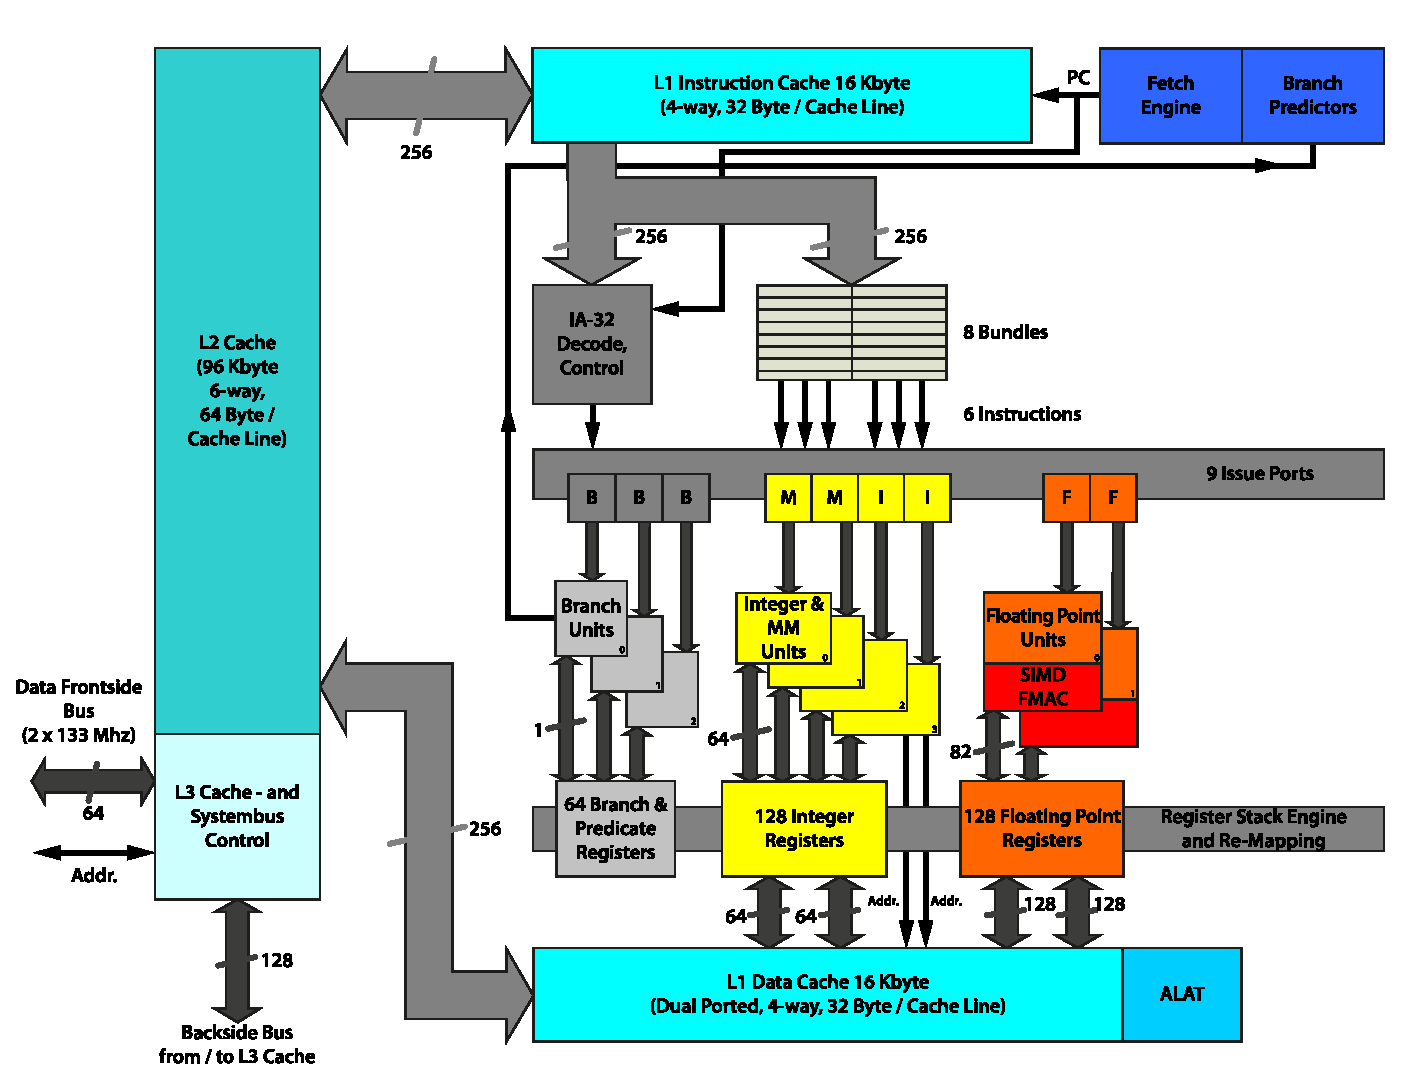
\includegraphics[scale=0.68]{mikroprozessoren2/Itanium_architecture.pdf}



\section{Parallelismus auf Thread-Ebene}



\section{Multicore/Manycore}



\section{Systemstrukturen}


\end{document}
